\documentclass[oneside]{book}
\usepackage{float}
\usepackage[UKenglish]{babel}
\usepackage{graphicx}
\usepackage{natbib}
\usepackage[colorlinks]{hyperref}
\usepackage[dvipsnames]{xcolor}
\usepackage{ amssymb, dsfont }
\usepackage{tikz}
\usepackage{dsfont}
\usepackage{mathrsfs}


\hypersetup{
  linkcolor  = Magenta,
  citecolor  = Aquamarine,
  urlcolor   = Periwinkle,
  linktoc    = page
}
\usepackage{algorithm}
\usepackage[noend]{algpseudocode}
\usepackage{amsmath,amssymb,bm}

\usepackage{enumitem}
\usepackage{subcaption}
\usepackage{wrapfig}
\usepackage{minted}  % Code embedding in document
\usepackage[none]{hyphenat}

\usepackage{mathtools}
\usepackage{verbatim}
\usepackage[export]{adjustbox}


\makeatletter
\newcommand\RedeclareMathOperator{%
  \@ifstar{\def\rmo@s{m}\rmo@redeclare}{\def\rmo@s{o}\rmo@redeclare}%
}
% this is taken from \renew@command
\newcommand\rmo@redeclare[2]{%
  \begingroup \escapechar\m@ne\xdef\@gtempa{{\string#1}}\endgroup
  \expandafter\@ifundefined\@gtempa
     {\@latex@error{\noexpand#1undefined}\@ehc}%
     \relax
  \expandafter\rmo@declmathop\rmo@s{#1}{#2}}
% This is just \@declmathop without \@ifdefinable
\newcommand\rmo@declmathop[3]{%
  \DeclareRobustCommand{#2}{\qopname\newmcodes@#1{#3}}%
}
\@onlypreamble\RedeclareMathOperator
\makeatother




\DeclarePairedDelimiter\ceil{\lceil}{\rceil}
\DeclarePairedDelimiter\floor{\lfloor}{\rfloor}

\DeclareMathOperator*{\argmax}{arg\,max}  % in your preamble
\DeclareMathOperator*{\argmin}{arg\,min}  % in your preamble 

\usepackage[nameinlink,noabbrev]{cleveref}
\newcommand*{\fullref}[1]{\hyperref[{#1}]{\Cref*{#1} -- \nameref*{#1}}}




% multiline comment
\renewcommand{\comment}[1]{}

% Number sets
\newcommand{\N}{\mathbb{N}} % Natural Numbers
\newcommand{\Z}{\mathbb{Z}} % Integers
\newcommand{\Q}{\mathbb{Q}} % Quotient
\newcommand{\R}{\mathbb{R}}	% Real Numbers
\newcommand{\C}{\mathbb{C}} % Complex Numbers 

% Probability
\newcommand{\freq}[1]{\text{Freq}\left(#1\right)} % Frequency
\newcommand{\pr}[1]{\mathbb{P}\left(#1\right)} % Probability
\newcommand{\expectation}[1]{\mathbb{E}_{#1}}
\newcommand{\E}[2][]{\expectation{#1}\left[#2\right]} % Expectation
\newcommand{\var}[1]{\mathbb{V}{\left(#1\right)}} % Variance
\newcommand{\cov}[1]{\text{Cov}{\left(#1\right)}} % Covariance
\newcommand{\corr}[1]{\rho{\left(#1\right)}} % Correlation

% Probability Distributions
\newcommand{\dber}[1]{\mathrm{Bern}(#1)} %Bernoulli
\newcommand{\dbeta}[1]{\mathrm{Beta}(#1)} %Beta
\newcommand{\dbin}[1]{\mathrm{Bin}(#1)} %Binomial
\newcommand{\dpoi}[1]{\mathrm{Poi}(#1)} %Poisson
\newcommand{\ddir}[1]{\mathrm{Dir}(#1)} %Dirichlet
\newcommand{\dgamma}[1]{\mathrm{Gam}(#1)} %Gamma
\newcommand{\dnorm}[1]{\mathcal{N}(#1)} %Normal/Gaussian
\newcommand{\dst}[1]{\mathrm{St}(#1)} %Student t
\newcommand{\duni}[1]{\mathrm{U}(#1)} %Uniform
\newcommand{\dwis}[1]{\mathcal{W}(#1)} %Wishart

% Linear Algebra
\newcommand{\vect}[1]{\bm{#1}} % vectors
\newcommand{\matr}[1]{\bm{#1}} % matrices and tensors
\newcommand{\tr}[1]{#1^{\top}} % transpose
\renewcommand{\sp}[2]{#1^{\top}#2}   %scalar product

% Analysis
\let\dbar\d \renewcommand{\d}{\mathrm{d}}
\newcommand{\D}{\,\mathrm{d}} % differential
\newcommand{\deriv}[2]{\frac{\d #1}{\d #2}} % derivative
\newcommand{\pd}[2]{\frac{\partial #1}{\partial #2}} % partial derivative
\newcommand{\set}[1]{\left\lbrace #1 \right\rbrace} % set
\newcommand{\where}{\ \middle\vert\;} % where
\newcommand{\abs}[1]{\left\vert #1 \right\vert} % absolute value
\newcommand{\norm}[2][]{{\left\Vert #2 \right\Vert}_{#1}} % norm
\input{jupyter}

\title{SP19 DL collaborative notes}
\author{
  The students of SP19 Deep Learning\\
  Editor: Alfredo Canziani\\
  NYU
}
\date{\today}

\begin{document}

\maketitle

\input{preface}
\chapter*{Instructions}

There are overall 42 hours of lectures.
For each hour there is a group of people assigned to summarise what happened in class \textbf{in roughly three pages}.
Each group is made of three students: two writers and a reviewer.

\subsection*{Writing directions}

Split your writing across the five parts of this document according to where it seems fit (see \nameref{chp:preface}).
Be consistent with the notation here specified.
\begin{itemize}[noitemsep,nolistsep]
\item Use \verb|\vect{}| and \verb|\matr{}| to decorate vectors and matrices respectively.
\item Start a new line \textbf{only and every time} you end a sentence with a period `.'; the \LaTeX\ engine will ignore this, but \verb|git| will love you.
\item Leave an empty line to start a new paragraph, and don't use the `\verb|\\|' break line (see \url{tex.stackexchange.com/a/225925/33287}).
\item Add date and group's authors name \textbf{as a comment}, after every \verb|\chapter|, \verb|\section|, and \verb|\subsection|.
\item The transposition symbol is obtained with \verb|^\top|. For example $(AB)^\top = B^\top A^\top$.
\end{itemize}

Feel free to create new chapters, sections, and subsections with corresponding labels \verb|\label{chp:}|, \verb|\label{sct:}|, and \verb|\label{ssc:}|.

\section*{Peer reviewing within groups}

Check for notation consistency, correctness, grammar, figure captioning, usage of \verb|\cref{}| instead of \verb|\ref{}|, \verb|\vect{}|, and \verb|\matr{}| to decorate vectors and matrices respectively, unnecessary use of bullet points or itemisations, missing references and use of links to papers PDF instead, usage of  $\pr{}$, $\E{}$, and $\var{}$ for probability, expectation, and variance respectively using \verb|\Pr|, \verb|\E{}|, and \verb|\var{}|, \verb|\mid| for the conditional vertical bar, missing backslashes for $\log, \exp, \max$ and any badly formatted functions, $\ast$ for convolutions, $\odot$ for elementwise multiplication, usage of \verb|\caption[Short caption]{Full caption}|, use of the correct transposition symbol obtained with \verb|\tr{}|, just to name a few.

\section*{Taking inspiration}

You can take inspiration from the work done by the students at NYU, who collectively wrote up the lecture notes in \href{https://www.overleaf.com/read/pchjywcxjkxn
}{this document} last year.
For example, you may reuse the following constructs, and others, at your convenience:
\[
\matr{X} = \begin{bmatrix}
    \rule[0.5mm]{0.8cm}{0.1mm} \; \vect{x}^{(1)} \; \rule[0.5mm]{0.8cm}{0.1mm} \\
    \rule[0.5mm]{0.8cm}{0.1mm} \; \vect{x}^{(2)} \; \rule[0.5mm]{0.8cm}{0.1mm} \\
    \vdots \\
    \rule[0.5mm]{0.8cm}{0.1mm} \; \vect{x}^{(m)} \; \rule[0.5mm]{0.8cm}{0.1mm} \\
\end{bmatrix}_{m \times n}
\matr{Y} = \begin{bmatrix}
    \rule[0.5mm]{0.8cm}{0.1mm} \; \vect{y}^{(1)} \; \rule[0.5mm]{0.8cm}{0.1mm} \\
    \rule[0.5mm]{0.8cm}{0.1mm} \; \vect{y}^{(2)} \; \rule[0.5mm]{0.8cm}{0.1mm} \\
    \vdots \\
    \rule[0.5mm]{0.8cm}{0.1mm} \; \vect{y}^{(m)} \; \rule[0.5mm]{0.8cm}{0.1mm} \\
\end{bmatrix}_{m \times K}
\]
\[
\hat{\matr{A}}\vect{x} =
\begin{bmatrix}
    \rule[0.5mm]{0.8cm}{0.1mm} \; \hat{\vect{a}}^{(1)} \; \rule[0.5mm]{0.8cm}{0.1mm} \\
    \rule[0.5mm]{0.8cm}{0.1mm} \; \hat{\vect{a}}^{(2)} \; \rule[0.5mm]{0.8cm}{0.1mm} \\
    \vdots \\
    \rule[0.5mm]{0.8cm}{0.1mm} \; \hat{\vect{a}}^{(m)} \; \rule[0.5mm]{0.8cm}{0.1mm} \\
\end{bmatrix}
\begin{pmatrix}
    \vrule height 0.6cm \\ \vect{x} \\ \vrule height 0.6cm
\end{pmatrix} =
\begin{pmatrix}
    \hat{\vect{a}}^{(1)} \vect{x} \\ \hat{\vect{a}}^{(2)} \vect{x} \\ \vdots \\ \hat{\vect{a}}^{(m)} \vect{x}
\end{pmatrix}_{m \times 1}
\]
\[
\matr{T}^{(1)}\vect{x} =
\begin{bmatrix}
    a_{1,1} & a_{1,2} & \dotsc & a_{1,k} & 0 & 0 & \dotsc & 0 \\
    0 & a_{1,1} & a_{1,2} & \dotsc & a_{1,k} & 0 & \dotsc & 0 \\
    0 & 0 & a_{1,1} & a_{1,2} & \dotsc & a_{1,k} & \dotsc & 0 \\
    \vdots & \vdots & \vdots & \ddots & \ddots & \ddots & \ddots & \vdots \\
    0 & \dotsc & 0 & 0 & a_{1,1} & a_{1,2} & \dotsc & a_{1,k}
\end{bmatrix}_{(n-k+1) \times n} =
\begin{pmatrix}
    \vect{a}^{(1)} \vect{x}_{1:1+k-1} \\ \vect{a}^{(1)} \vect{x}_{2:2+k-1} \\ \vdots \\ \vect{a}^{(1)}  \vect{x}_{n-k+1:n}
\end{pmatrix}_{(n-k+1) \times 1}
\]

Have fun!


\tableofcontents

%%%%%%%%%%%%%%%%%%%%%%%%%%%%%%%%%%%%%%%%%%
% NEW PARTS
%%%%%%%%%%%%%%%%%%%%%%%%%%%%%%%%%%%%%%%%%%

%%%%%%%%%%%%%%%%%%%%%%%%%%%%%%%%%%%%%%%%%%
\part{Paradigms}\label{prt:prdg}
%%%%%%%%%%%%%%%%%%%%%%%%%%%%%%%%%%%%%%%%%%
\chapter{Motivation}\label{chp:motivation}
% Authors: Ethan Perez, Diego Casabuena, Yi Tang. 2/3/18.

\section{Ideas for “Generic” Feature Extraction}\label{ssec:generic-feature-extraction}
% Authors: Ethan Perez, Diego Casabuena, Yi Tang. 2/3/18.

For much of its history, the field of Artificial Intelligence has viewed high-quality hand-crafted, task-specific features as the key to machine intelligence.
In contrast, more recent years have witnessed the popularity and successes of \textit{learned} and generic features.
Preceding deep learning, many other approaches (such as SVM) for extracting generic features have been explored.

Generally speaking, feature extraction often consists of expanding the input's representational dimension such that the expanded features are more likely to be linearly separable; intuitively, points in higher dimensional space are more likely to be linearly separable due to the increase in the number of possible separating planes.
To this end, feature extracting algorithms may learn some $f(x)=\sum_i w_i \phi_i (x)$, where $w_i$ are the learned coefficients and $\phi_i$ are some chosen basic features.
To form $\phi_i (x)$, there are (among others) five common approaches:

\begin{enumerate}
    \item \textbf{Space tiling}: To use linear combinations of engineered features.
    In this method $\phi_i(x) = \phi(x,u_i)$ are used where $u_i$ spreads over the domain.
    However, this method does not scale that well in the number of input dimensions $d$, as one would need $n^d$ bumps/mappings/sub-functions to spread a grid of size $n$ in each dimension.

    \item \textbf{Random projections}: To compose random projection matrices and use them to get features.
    Randomly projected features turn out to perform well in practice.

    \item \textbf{Polynomial classifier}: To use monomials as $\phi_i$.
    This is a very common method of involving additional dimensions.
    Given data of dimension $d$, one can compose a polynomial whose terms are the products of particular dimensions.
    For example, for $d = 2$ (and data $(x_1, x_2)$), the polynomial would assume the form
    \begin{equation*}
        w_0 + \sum_{a \in \mathbb{N}^*} w_{1, a} x_1^a + \sum_{b \in \mathbb{N}^*} w_{2, b} x_2^b + \sum_{c_1, c_2 \in \mathbb{N}^*} w_{3, c_1, c_2} x_1^{c_1} x_2^{c_2}
        \text{.}
    \end{equation*}
    % Doesn’t scale well in high dimensions.
    % Need to compute polynomial features of your input (how many are there?)
    One can further limit the degree of the polynomial for computational efficiency.
    For instance, a degree-2 polynomial (for $d = 2$) would have the form $w_0 + w_{1, 1} x_1 + w_{2, 1} x_2 + w_{1, 2} x_1^2 + w_{2, 2} x_2^2 + w_3 x_1 x_2$.

    \item \textbf{Radial Basis Functions (RBF)}: To use functions whose value depends only on the distance from the variable to a given point.
    For example, a commonly used function family is $\phi_i(x)=e^{-{\|x-u_i\|}^2}$.

    \item \textbf{Kernel machines}: Based on a kernel function that satisfies the Mercer condition.
    More specifically, one could use $\phi_i(x) = K(x, u_i)$ where $K$ is a continuous, symmetric, positive-definite kernel function (which indicates the matrix $[K(x_i, x_j)]_{i, j}$ is positive definite, where $x_i$ are the sample points).
    In essence, taking $\phi_i(x) = K(x, x_i)$ is equivalent to a 2-layer neural network that uses tiling, that locates exactly around the training sample points (as $u_i = x_i$).
\end{enumerate}

As a sidenote, it is not hard to see how a single layer classifier of the sorts discussed above may potentially require infinite dimensions.

\section{History of Deep Learning}\label{ssec:history}
% Authors: Ethan Perez, Diego Casabuena, Yi Tang. 2/3/18.

The seeds of deep learning date back at least to the invention of the perceptron by Frank Rosenblatt in 1957.
The perceptron is a binary classifier that attempts to linearly separate the data via weights on the input features learned via supervision.
The perceptron may be viewed as a single-layer neural network, and initially it seemed to be a promising statistical learning approach for classification problems (e.g., image classification).
However, in 1969, Marvin Minksy and Seymour Papert showed that perceptrons cannot compute or represent some functions, for example the XOR function.
This result only held for single-layer, linear perceptrons, and not in the case of non-linear multi-layer perceptrons.
Despite the potential of the perceptron, the above result discouraged further research into the method.
Thus, the field as it was known died and its place in research was taken by the related (or rebranded) fields of statistical learning theory and adaptive filters.
These would continue to make further developments in the following years.

In the early 1980s, several exciting results re-popularized neural networks for some time.
In 1982, John Hopfield discovered interesting mathematical connections between perceptrons (more generally neural networks) and concepts in physics.
Soon after, in 1983, Geoffrey Hinton developed the Boltzmann machine, publishing the method in AAAI, a top tier conference in AI at the time, in a paper titled ``\href{https://papers.cnl.salk.edu/PDFs/Optimal\%20Perceptual\%20Inference\%201983-646.pdf}{Optimal Perceptual Inference}.''
% Paper URL: https://papers.cnl.salk.edu/PDFs/Optimal%20Perceptual%20Inference%201983-646.pdf
The Boltzmann machine was one of the first methods that could train a \textit{multi-layer} perceptron.
Later, in 1985, Rumelhart, Hinton, Lecun, and several others discovered the backpropagation algorithm for training multi-layer perceptrons.
Backpropagation is conceptually simple: repeatedly apply the chain rule starting from the gradients of the last layer of the perceptron until the first layer.
Interestingly, this algorithm had not been discovered before this time, given that previous neural networks had largely been formulated with binary, thresholding activations, which are non-differentiable.
However, these activations could be swapped for other differentiable activations, such as sigmoid functions (a kind of soft thresholding function) or rectified linear units, in order to facilitate backpropagation.
Notably, this non-linear optimization procedure faces the theoretical problem of reaching local minima.
However, Hinton showed it was possible to successfully train neural nets anyways -- that in practice, the solutions found by backpropagation perform reasonably well.

Despite these successes, other models (such as the Support Vector Machine) in the 1990s and 2000s overtook neural networks in popularity.
It was not until the early 2010s that deep learning became popular yet again, with breakthrough successes in speech recognition and image classification.

\section{Hierarchical Representation}\label{ssec:hierarchical-representation}
% Authors: Ethan Perez, Diego Casabuena, Yi Tang. 2/3/18.

Deep learning has a hierarchical nature.
From simpler structures we derive more complex ones.
In a neural network, the layers are essentially stages of non-linear feature transformations.
This inherent hierarchy of representations can also be found on the Mammalian Visual Cortex, where the different sections of the Cortex understand increasingly complex levels of information about a visual input (as can be seen in \cref{fig:deep-learning-hierarchical-features}).

\begin{figure}[ht]
\centering
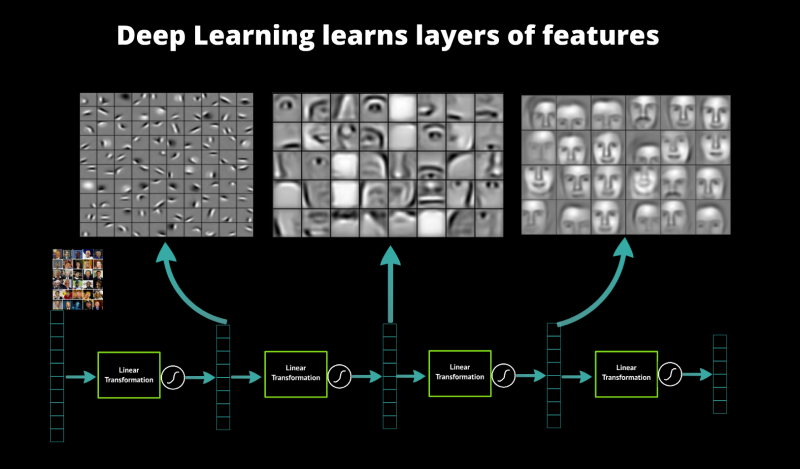
\includegraphics[width=0.85\linewidth]{figs/dl_features.png}
% Figure from: https://www.datasciencecentral.com/profiles/blogs/a-primer-on-deep-learning
\caption{In the figure above we see how the layers closer to the input of the network are more abstract, and that those closer to the final layer are most concrete and interpretable.}
\label{fig:deep-learning-hierarchical-features}
\end{figure}

In a neural network, we feed the output of one layer onto the input of the next.
Layers are composed of linear transformations followed by non-linear activation functions.
Altogether, this system allows the network to learn the non-linear features of interest.

Hierarchical feature representations are intuitive for many domains, as our world is compositional (the whole is often a function of its parts).
For example, consider the following domains:
\begin{itemize}
    \item \textbf{Image recognition}: Pixels compose edges, which compose ``textons'' (i.e., multi-edge shapes), which compose motifs, which compose parts, which finally compose whole objects.
    Algorithms may learn to understand what an object looks like by learning a function mapping from pixels to a slightly higher level representation such as edges, then to textons, etc., until a high enough level representation is formed to represent whole objects.
    Indeed, there is evidence from neuroscience that the visual cortex represents objects in such a hierarchical manner in animals.

    \item \textbf{Language}: Language is inherently compositional as well.
    The meaning of a book is a composition of the meanings of its chapters, then paragraphs, then sentences, then phrases, then words (then even characters).
    While not all language is compositional (a ``heavy accent'' has nothing to do with weight), it often is, as language is how humans represent the world which is often compositional.

    \item \textbf{Speech}: In speech, a sample composes a band, which composes a sound, which compose phones, then phonemes, then whole words and sentences.
    The capacity for each component of this hierarchy in speech is what enables hierarchical models to represent very high-level features of sound by simply forming consecutively higher representations over what is ultimately a series of bytes.
\end{itemize}

\begin{document}
\chapter{Backpropagation}\label{chp:Backpropagation}
% Authors: Vaibhav A Gadodia, Yair Schiff, Goutham Panneeru
% Lecture date: 02.04.2019

\section{Motivation}
% Authors: Vaibhav A Gadodia, Yair Schiff, Goutham Panneeru
% Lecture date: 02.04.2019

Backpropagation is the process of finding the gradients of the weights and biases of a neural network using the chain rule. Backpropagation process starts with the last layer of the neural network, and continues by moving backwards.
It provides a disciplined way to train neural networks using gradient descent.
At the heart of backpropagation is the use of the chain-rule for calculating gradients of composed functions.
Neural networks model the composition of linear and element-wise non-linear transformations, and so the calculation of gradients to be used in model training via the chain-rule is a natural choice.

\section{Automatic Backpropagation}
% Authors: Vaibhav A Gadodia, Yair Schiff, Goutham Panneeru
% Lecture date: 02.04.2019

Given the importance of gradients in training neural networks, frameworks, such as torch, keep track of and pre-calculated derivatives of commonly used functions or modules.
The PyTorch library has both functional (stateless) and class forms of frequently used neural network modules.
Class forms of these modules have constructors and forward propagation methods, and generally there is no need to compute the gradient of functions, as it is already computed and maintained in the class.
Thus in module classes, state consists of two variables: one holding the result of forward propagation from the module to its successor nodes, and the other one holding the derivatives with respect to inputs and weights in the module to be passed backwards during backpropagation.

\section{Common Modules}
% Authors: Vaibhav A Gadodia, Yair Schiff, Goutham Panneeru
% Lecture date: 02.04.2019

Below are some of the common modules and the gradients of a cost function $E(W)$, which is parameterized by the weights, $W$ of the neural network connections.

\subsection{Linear Module}
% Authors: Vaibhav A Gadodia, Yair Schiff, Goutham Panneeru
% Lecture date: 02.04.2019

The linear module represents the multiplication of an input vector by a matrix of weights $W$ and thus expresses a linear transformation of inputs.
More formally, the forward propagation of this module can be written as: $$X_{out} = WX_{in}$$ where $X_{in}$ is a $p$-dimensional vector of inputs to the module, $W$ is a $d \times p$-dimensional matrix of weights, and $X_{out}$ is a $d$-dimensional vector that is the output of the module.
Now in order to back propagate through a network, we will need to calculate the Jacobian with respect to $X_{in}$ and with respect to $W$.
To do so, we employ the chain rule: $$\frac{\partial E}{\partial X_{in}} = \frac{\partial E}{\partial X_{out}}\frac{\partial X_{out}}{\partial X_{in}} = \frac{\partial E}{\partial X_{out}}W$$ Given the dimensions above, this will be a $1 \times p$ row vector of partial derivatives. To turn this vector into a column vector, we take its transpose: $$\left(\frac{\partial E}{\partial X_{in}}\right)^\top = W^\top \left(\frac{\partial E}{\partial X_{out}}\right)^\top$$ Thus, we see that in the linear module, for the input vector $X_{in}$, we multiply by the weight matrix $W$ on forward propagation and by $W^\top$ on backward propagation.
To calculate the partial derivative of E w.r.t $X_{in}$, we need to calculate the gradient w.r.t each entry of the input vector. Consider the i^{-th} entry of $X_{out}$ which has the following equation:
$$X_{out,i} = \sum_{j}(W_{ij} * X_{in,j})$$ Here each entry of $X_{in}$ i.e., $X_{in,j}$ influences all the entries in $X_{out}$ through various W entries which gives rise to: $$\frac{\partial E}{\partial X_{in, j}} = \sum_{i}\frac{\partial E}{\partial X_{out,i}} \frac{\partial X_{out,i}}{\partial X_{in,j}} $$

Now, to calculate the gradient with respect to the weight matrix $W$, we begin by looking at the partial derivative with respect to an individual entry $W_{ij}$ of the weight matrix. The only factor influenced when $X_{out,i}$ changes w.r.t $W_{ij}$ is $X_{in,j}$:  $$\frac{\partial E}{\partial W_{ij}} = \frac{\partial E}{\partial X_{out, i}}\frac{\partial X_{out, i}}{\partial W_{ij}} = \frac{\partial E}{\partial X_{out, i}}X_{in, j}$$ Extrapolating from here, the Jacobian w.r.t the full weight matrix can be expressed as an outer product: $$\left(\frac{\partial E}{\partial W}\right)^\top = \left(\frac{\partial E}{\partial X_{out}}\right)^\top X_{in}^\top$$

\subsection{Hyperbolic Tangent - tanh}
% Authors: Vaibhav A Gadodia, Yair Schiff, Goutham Panneeru
% Lecture date: 02.04.2019

The tanh module is a popular non-linearity. Other commonly used non-linearities, such as the sigmoid function and rectified linear unit (ReLU), follow a similar pattern to tanh.

To execute non-linear transformations of the input data, in addition to the linear modules, neural nets employ point-wise non-linearities, such as the tanh function.
The hyperbolic tangent is computed as follows: $$\mathrm{tanh}(x) = \frac{2}{1 + \exp(-x)} - 1 = \frac{1 - \exp(-x)}{1 + \exp(-x)}$$ Given this non-linearity is applied element-wise, for forward propagation, we can look at an individual index $i$ of the output vector $X_{out}$: $$X_{out, i} = \mathrm{tanh}(X_{in, i} + \beta_i)$$ where $\beta$ is a bias vector added to the input vector.
For backpropagation on the input vector and bias, we again use the chain rule: $$\left(\frac{\partial E}{\partial X_{in}}\right)_{i} = \left(\frac{\partial E}{\partial X_{out}}\right)_{i}\mathrm{tanh}'(X_{in, i} + \beta)$$ $$\frac{\partial E}{\partial \beta_i} = \left(\frac{\partial E}{\partial X_{out}}\right)_{i}\mathrm{tanh}'(X_{in, i} + \beta)$$ where the derivative $\mathrm{tanh}'$ is: $$\frac{d}{dx}\mathrm{tanh}(x) = 1 - \mathrm{tanh}^2(x)$$

\subsection{Euclidean Distance Module}
% Authors: Vaibhav A Gadodia, Yair Schiff, Goutham Panneeru
% Lecture date: 02.04.2019

Euclidean distance is a metric for determining proximity of two points in Euclidean space.
This module is often used as the final layer of a neural network to compute the distance between a prediction and a ground truth label, where it is also commonly known as the mean squared error (MSE).

In forward propagation, the output, scalar quantity is calculated as one half the $\ell_2$ norm of the difference between the input vector $X_{in}$ and the provided label $Y$, squared: $$X_{out} = \frac{1}{2}||X_{in} - Y||^2$$ Back propagation to the input vector and label is symmetric: $$\frac{\partial E}{\partial X_{in}} = X_{in} - Y$$ $$\frac{\partial E}{\partial Y} = Y - X_{in}$$

\subsection{Y-connector and Addition Modules}
% Authors: Vaibhav A Gadodia, Yair Schiff, Goutham Panneeru
% Lecture date: 02.04.2019

The Y-connector and Addition modules are related, in that the two mirror each other on forward and backward propagation.
The Y-connector module takes an input vector and \textit{copies} it to two or more output vectors.
The Addition module, on the other hand, takes two or more input vectors and adds them to form a single output vector.

On the backwards pass, the Y-connector needs to sum the partial derivatives with respect to each of the its output vectors in order to calculate the gradient with respect to the input vector.
The Addition module need only copy the partial derivative of the output vector to each of its inputs, thus giving rise to the mirrored pattern referenced above.
More formally, the Y-connector module can be formulated as follows:
\begin{itemize}
    \item Forward: $\forall k \in [1..K]: \ X_{out}^{(k)} = X_{in}$
    \item Backward: $\frac{\partial E}{\partial X_{in}} = \sum_k{\frac{\partial E}{\partial X_{out}^{(k)}}}$
\end{itemize}
The Addition module can be expressed as:
\begin{itemize}
    \item Forward: $X_{out} = \sum_k{X_{in}^{(k)}}$
    \item Backward: $\forall k \in [1..K]: \ \frac{\partial E}{\partial X_{in}^{(k)}} = X_{out}$
\end{itemize}

\subsection{Switch Module}
% Authors: Vaibhav A Gadodia, Yair Schiff, Goutham Panneeru
% Lecture date: 02.04.2019

This module takes in $k$ input vectors $X_{in}^{(k)}$ and a discrete-valued $Y$ variable, which acts as a switch, selecting one of the $k$ inputs to be copied to the output vector $X_{out}$.
At first glance, this module may seem non-differentiable, but further examination reveals that indeed the gradient can be calculated by simply passing the gradient of the output to the input vector that was selected by $Y$ and setting the gradient for all other input vectors to zero.
For this module, the state variable that maintains information about forward propagation is essential to back propagation as well, since it allows for the gradient to flow backwards through the selected input.

\subsection{SoftMax Module}
% Authors: Vaibhav A Gadodia, Yair Schiff, Goutham Panneeru
% Lecture date: 02.04.2019

The SoftMax module is an important module that is often used in multi-class supervised learning.
Known also as the Boltzmann-Gibbs distribution by the Physics community, this module takes as an input a vector $X_{in}$ and produces an output vector $X_{out}$ that resembles a probability distribution, as each output component $X_{out, i} \in [0, 1]$ and they all sum to 1: $||X_{out}||_1 = 1$.
The softmax equation for a given index $j$ of the output vector is expressed as follows: $$X_{out, j} = \frac{\exp(\beta X_{in, j})}{\sum_i{\exp(\beta X_{in, i})}}$$ Back propagation for each component $i$ of the input vector depends on whether that component is equal to $j$ or not.
More formally:
\begin{itemize}
    \item $i = j$: $\frac{\partial X_{out, j}}{\partial X_{in, i}} = \beta X_{out, j}(1 - X_{out, j})$
    \item $i \neq j$: $\frac{\partial X_{out, j}}{\partial X_{in, i}} = -\beta X_{out, i}X_{out, j}$
\end{itemize}
\end{document}
 %backprogation ch 5
% Lecture date: 04/15/2019, part one
% Authors: Yunhao Li, Geyi Zhang, He Li (editor)
% Time interval: 00:21:00 - 01:15:00
\chapter{Unsupervised Learning}

\section{Introduction}

\subsection{Machine Learning and the Cake Analogy}

Machine learning techniques such as supervised learning (which only predicts human-provided labels), and reinforcement learning (which only predicts a value function), are too narrow to create human-level intelligent machines. Unsupervised learning (or self-supervised learning to be exact), however, with its millions of bits of information per sample, can be used to train highly complex machines without human supervision.

Like supervised learning, self-supervised learning learns a function from pairs of inputs and outputs. However, instead of having annotators manually label the data, self-supervised learning automatically generates labels by extracting weak annotation information from the input data and predicting the rest. In this way the model can independently learn semantic feature representations of data, which can be further used in other tasks.

There are some examples where supervised learning is not suitable and we can use unsupervised learning techniques:
\begin{itemize}
    \item \textbf{Machine translation for any given language pair}: There are about 5k-7k languages, and we cannot do a supervised problem of learning $n^2$ language-to-language pair translators. A unsupervised learning way to do this is using a encoder-decoder structure we encode any language into a intermediate representation space ($n$ encoder) and decode from this internal representation to the chosen language ($n$ decoder).

    \item \textbf{Learning with very small amount of data}: There is a lot of situation that we don't have a lot of labeled data. People want to detect rare occurrences of things. Train a system to detect rare diseases in medical images or train the automatic driving systems where you cannot to exhaust every cases.

    \item \textbf{Combining deep learning with reasoning}: In some case we need to train systems to reason, not just perceive. Human have a pretty good model that predicts what may happen. So we can know the result without trying it. This model is acquired by observing which is a form of unsupervised learning.
\end{itemize}

Today’s AI technologies can easily classify images and recognize voices, but cannot perform tasks such as reasoning the relationship between different objects or predicting humans’ movements. That is where unsupervised learning can fill the blanks. The reason we need unsupervised learning is the fact that the number of the amount of the data we ask machine to predict is sort of different. These different paradigms of learning are very different.

\begin{itemize}
    \item In the reinforcement learning, you ask machine to predict a reward(cost) of a particular sequence of action. The system just gets a reward instead of much information in the end. It is a very sparse feedback, which means the number of trials needed is very large because in every trial you only give it a little information.

    \item In supervised learning, you give $10-10,000$ bits per sample. When doing ImageNet classification, for example, there is $1,000$ categories. The information is $10$ bits.

    \item In unsupervised learning, much more information has be used.
\end{itemize}

There is a analogy of machine learning and the cake: almost everything we learn we learned in unsupervised learning. We learn a little bit through supervised learning, and we learn a tiny bit through reinforcement learning.

\begin{figure}[ht]
\centering
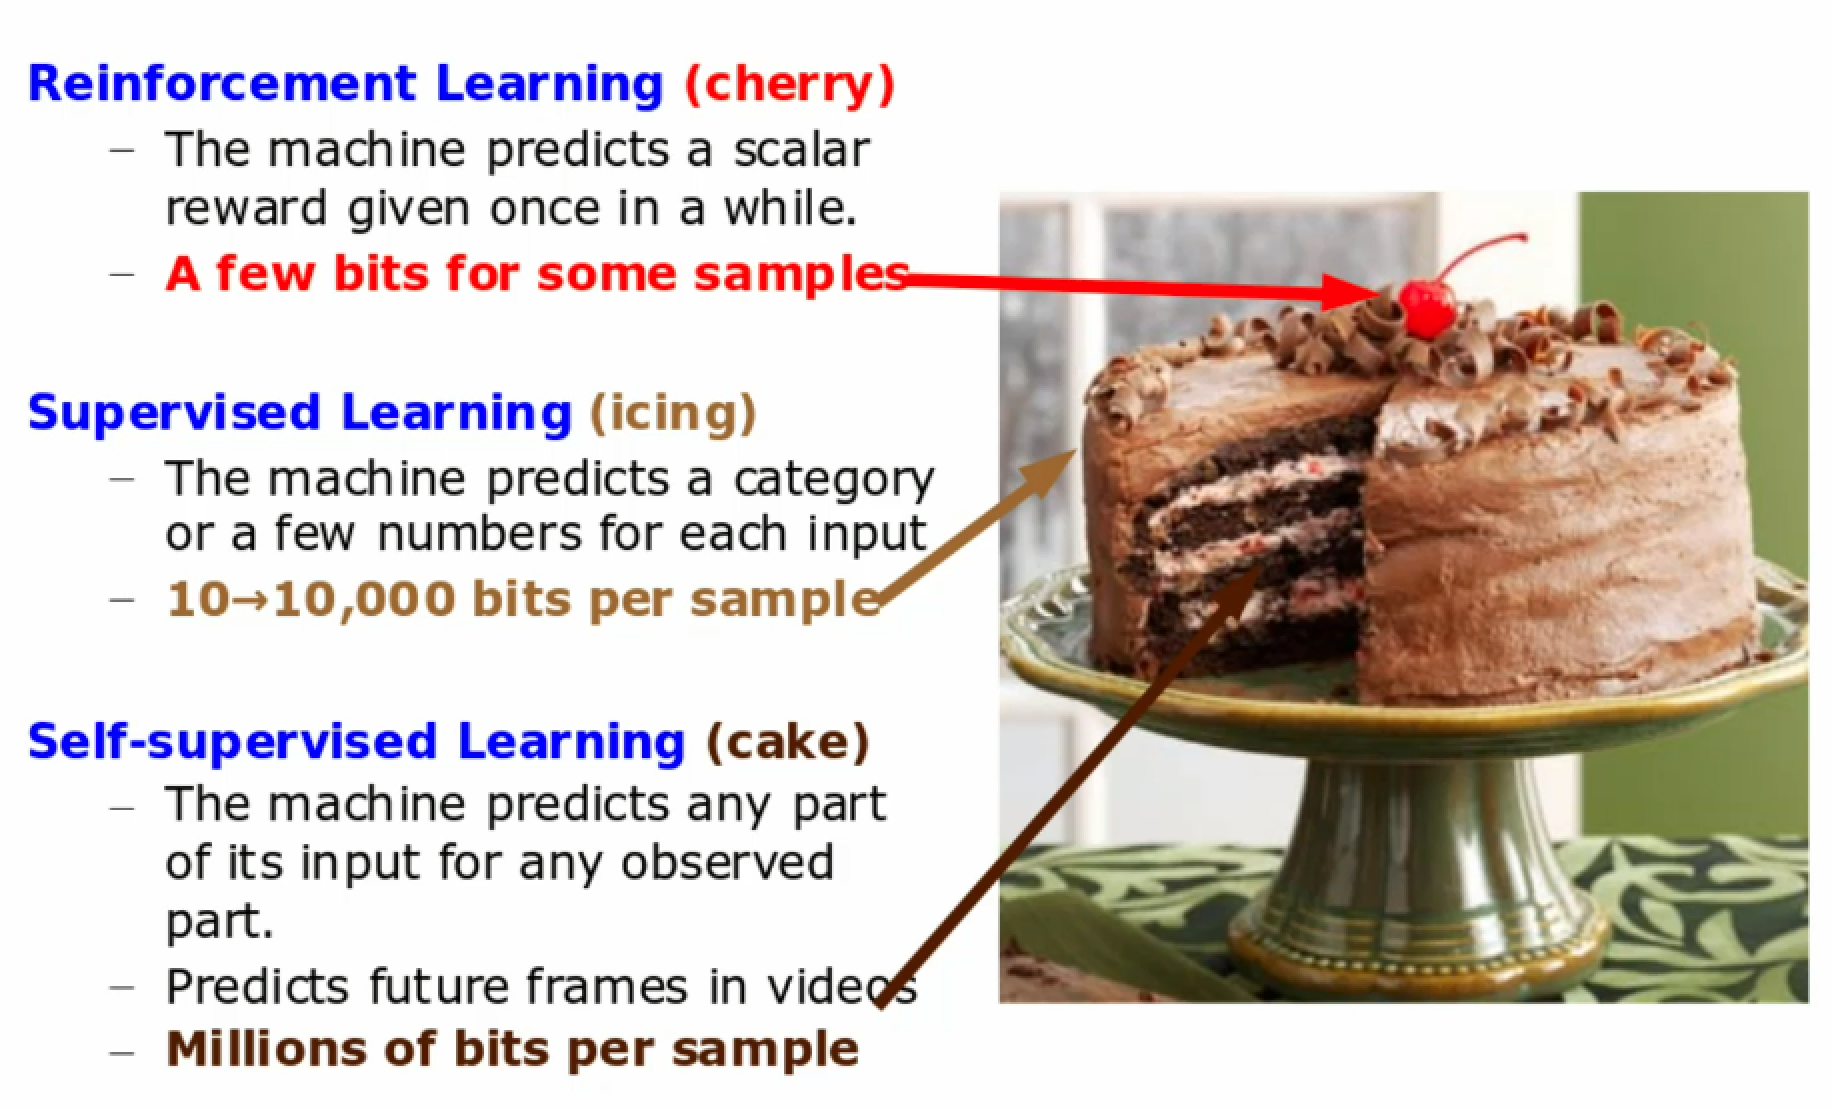
\includegraphics[height=7cm]{lectures/10-a/cake.png}
\caption{Cake Analogy}
\label{fig:label}
\end{figure}

\subsection{How do we do unsupervised learning?}

Prediction is kind of a reconstruction. For example, you can train a system to predict the end of a video from the beginning. But you can also do it in the other direction(given the end, predict what happened before). Completing the missing information, filling the blanks, that's the purpose of unsupervised learning.

So there is a problem: if I ask you to predict the future of a video with given video clips, many plausible things can happen. There is no single correct answer for this. The energy based learning will be useful. We need to construct a predictor that can predict multiple things, not just one single future prediction. The world is not entirely predictable. There is a lot of uncertainty. The question is, how do construct machine to predict things. The immediate answer is we can predict a distribution instead of predicting a single point.(e.g. Put a pen on table and let it go. The pen falls in a different direction every time. The directions is in a distribution) If you want to predict a frame of video, there is a distribution of images. You will have to parameterize the distribution of images. The basic possible to parameterize the distribution. We don't have density models or condition models of natural images. The main issue is that we don't know how to represent normalized distributions. Giving a quality of goodness or badness to a particular image is maybe possible, but training this into a distribution is very hard. That is one reason for introducing energy based models.

\section{Energy-based Unsupervised Learning}

\subsection{Introduction}

The way to make multiple predictions, or to build a model makes multiple predictions is through the latent variable. Imagine that for a predictor we are going to train, the $x$ are the frames of the video tape, $y$ is the feature of that particular video tape, and we will have an extra input $z$ to the function. What we would like to have is training the system in such a way that, when the latent variable varies over a particular set, the output varies over the set of all plausible predictions. For a particular $z$, the predicted next frame $y^\prime$ and the actual $y$ observed, by tweaking the latent variable, the model is to predict the actually observed $y$.

The idea of latent variable model is that, we have a latent variable of which value is not known, but through optimization, you are able to find the value of it that makes the best prediction.

What to do here is to measure the distance, try to figure out what is the value $z$ within the set, that would minimize the distance between the prediction $y^\prime$ and the $y$ observed. It may not actually be equal, so you will train the network to make these two as closet as possible, for the particular $z$.

\subsection{Shape the Energy Function}

The energy-based unsupervised learning is identical to energy-based models, except here are $Y_1$ and $Y_2$ instead of $X$ and $Y$. We train the network to figure out the structure of $Y$, where the energy function will takes low values of the data points nearby and higher values that aside. Capturing those dependencies through the energy function allows you to predict any subset of variables from any other subset of variables.

Making energy low on the training samples is easy, which can be achieved just by showing the training data and tweaking the parameters to make energy low on them. The most tricky part is how to ensure the energy is higher outside the training data. There are several ways to do that as shown below.

\begin{enumerate}
    \item \textbf{Constant and Constraint}: The volume of the space that your energy function can give low values to is limited or constant. For example, normalized probability model satisfy this condition, because if at one point the probability goes up, there would be another point that goes down to maintain the normalized distribution. Since the whole volume of probability is constant which equal to $1$, the volume of low energy stuff is constant as well.
    \begin{enumerate}
        \item \textbf{Gaussian Mixture Model}.
        \item \textbf{Principal Component Analysis}: There is one-hot vector $z$ multiplied by matrix, and goes into euclidean distance, let $E(y, w)= \|y-wz \|^2$. Compute $f(y)= \arg\min_z E(y,z)$ , select $w$ that is a prototype closest to $y$ by inferring latent variable $z$. See Figure~\ref{fig:unsupervised-energy-1} for an illustration.
        \item \textbf{K-means}: The energy function has $k$ valleys, not more than $k$, the volumes is bounded to constant once $k$ is decided.
    \end{enumerate}
    
    \begin{figure}[htb]
    \centering
    \begin{subfigure}[b]{0.4\textwidth}
        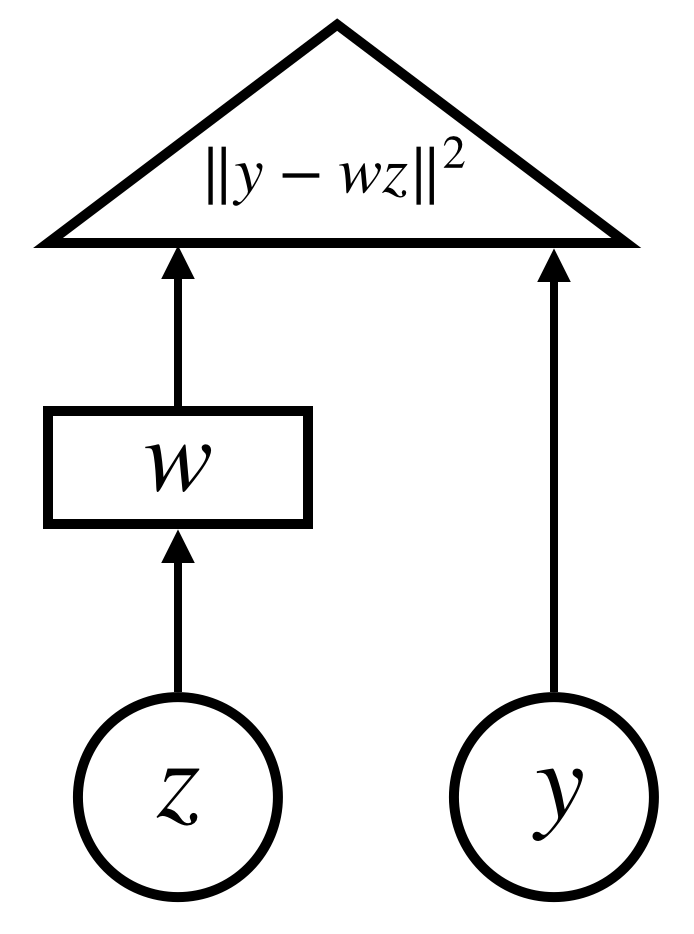
\includegraphics[height=\textwidth]{lectures/10-a/energy-based-1.png}
        \caption{Principal Component Analysis}
        \label{fig:unsupervised-energy-1}
    \end{subfigure}
    \begin{subfigure}[b]{0.4\textwidth}
        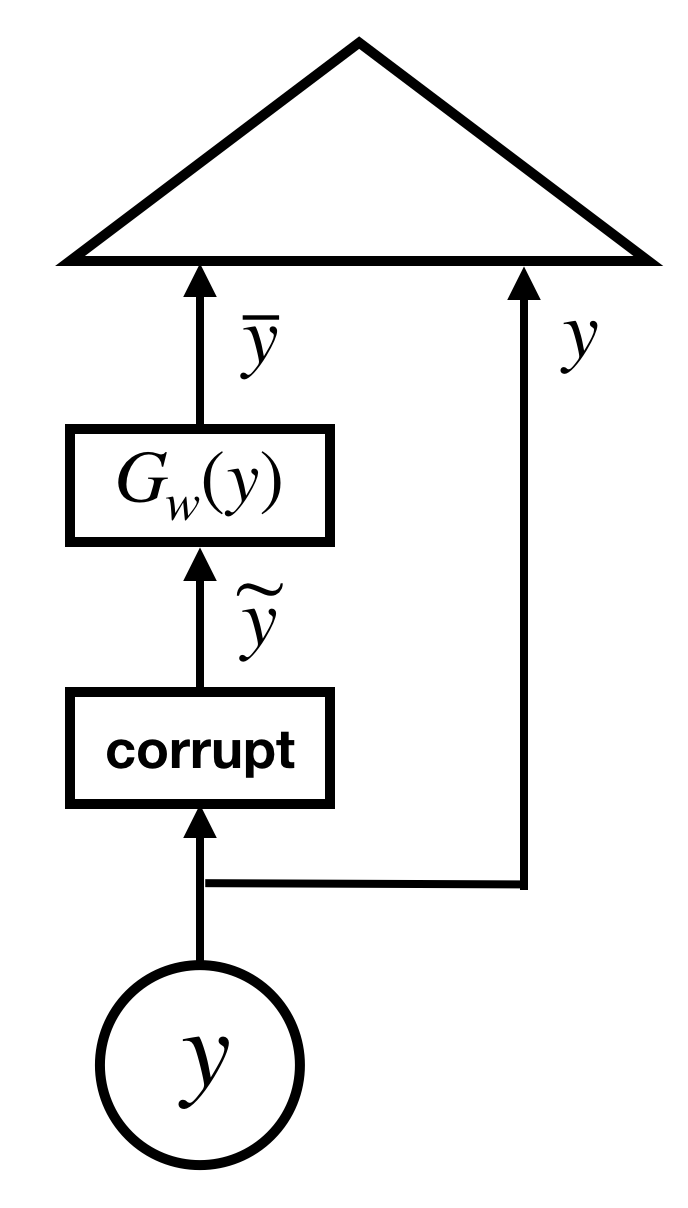
\includegraphics[height=\textwidth]{lectures/10-a/energy-based-2.png}
        \caption{Denoising Autoencoder}
        \label{fig:unsupervised-energy-2}
    \end{subfigure}
    \caption{Shape the Energy Function}\label{fig:unsupervised-energy}
    \end{figure}

    \item \textbf{Push Down and Push Up}: Here are two methods that push down energy of data points while push up elsewhere or on chosen locations, both invented by physicists.
    \begin{enumerate}
        \item \textbf{Monte-Carlo Sampling}: Replace integral with discrete sum, draw samples and take average.
        \item \textbf{Variational Approximation}: Replace $P(y, w)$ distribution with another distribution $Q$ that is easier to compute (e.g. Gaussian), and minimize the Kullback–Leibler divergence between $P$ and $Q$.
    \end{enumerate}

    \item \textbf{Minimize Gradient and Maximize Curvature}: It is impractical. We need to make energy flat around data points, which means the derivative being zero, and the second derivative as large as possible. In other words, "Compute the gradients with respect to parameters of the sum of the diagonal terms which is the trace of the Hessian function with respect to the inputs."

    \item \textbf{Denoising Autoencoder}: This method is useful. How it works is we have an input $y$ and corrupt it with noise, then pass the corrupted $y$ through a parameterized function $G$, eventually the energy function compares the uncorrupted $y$ and $G(\bar{y})$, gives the distance $\bar{y}$ is away from the manifold which is also the reconstruction error. The noise $\bar{y}$ will have high energy. There are two problems with this method, the first one is that it is hard to know what noise to add. There are too many ways to corrupt an input, you may not be able to cover all that expand the entire high-dimensional space outside your manifold. The second one it that there is no guarantee the model is going to learn exactly what you taught, for instance, the catastrophic scenario is that the points reconstructed go in circle. See Figure~\ref{fig:unsupervised-energy-2} above for an illustration.
\end{enumerate}
\chapter{Unsupervised Learning}
% Authors: Kevin Ayuque (Editor), Bin Wang, Ding Wang
% Lecture  date: 4/15/2019 part 2

\section{Energy-based Unsupervised Learning}
% Authors: Kevin Ayuque (Editor), Bin Wang, Ding Wang
% Lecture date: 4/15/2019 part 2

At a high level, many unsupervised models can be viewed as a scalar-valued energy function $E(Y)$ that operates on input data vector $Y$.
The energy function is subject to learning.
Training an unsupervised model consists in searching for an energy function within a family ${E(Y, W), W \in \mathcal{W}}$ indexed by a parameter $W$.
Both $E(Y)$ and $E(Y, W)$  are designed to produce low energy values when $Y$ is similar to the training data and high energy values when $Y$ is dissimilar to the training data.

Energy-based models have been used to capture dependencies over variables by defining an energy function.
The energy function associates each configuration of the variables with a scalar energy value. 
Lower energy values should be assigned to more likely or plausible configurations and conversely higher values to others. Figure \ref{figure1} shows an example of samples in the manifold, where 
\begin{equation}
    Y_2 = Y_1^2
\end{equation}
\begin{figure}[H]
        \centering
        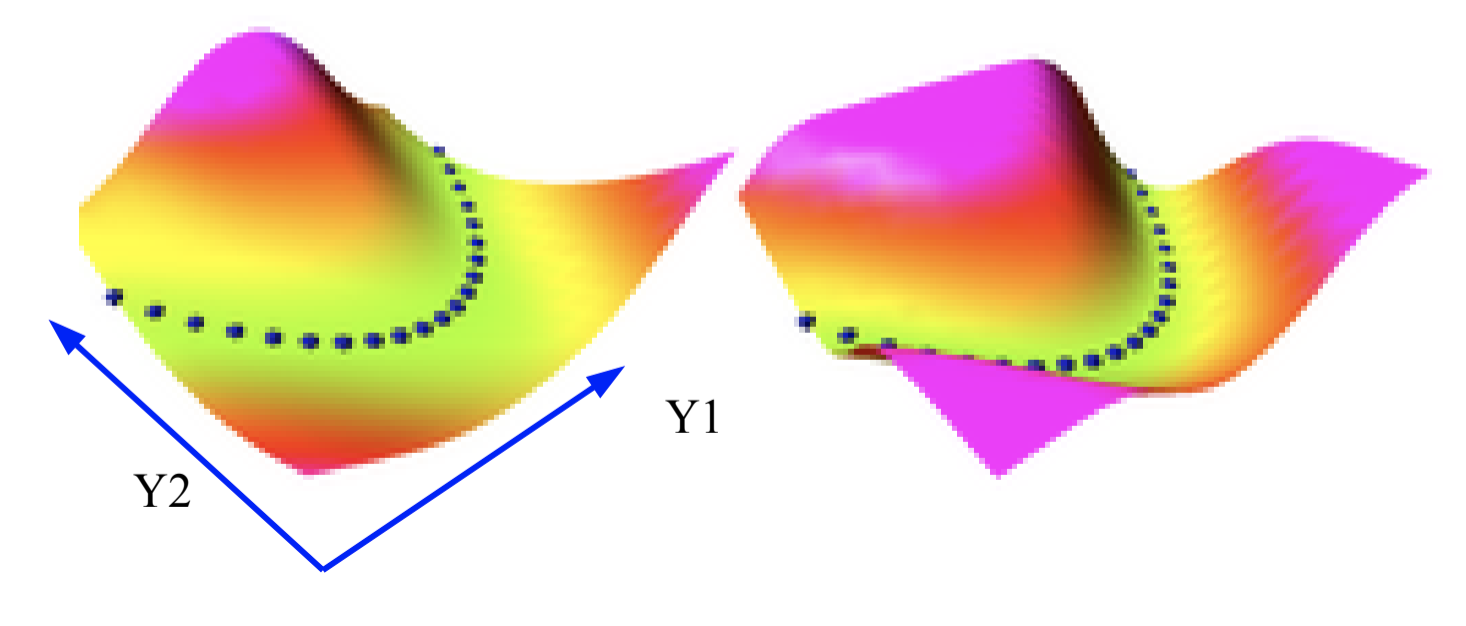
\includegraphics[width=\textwidth]{lectures/10-b/image/pic2.png}
        \caption{Example: The samples live in the manifold}
        \label{figure1}
    \end{figure}
Making the energy low on the samples is easy (through back-propagation). But how do we make it high everywhere else? Pulling up the energies of unobserved points in high dimensional spaces is often very difficult and even intractable. 
Probabilistic models use a particular method for pulling up the energy of unobserved points that turn out to be very inefficient in many cases.

\subsection{Strategies to Shape the Energy Function}
% Authors: Kevin Ayuque (Editor), Bin Wang, Ding Wang
% Lecture date: 4/15/2019 part 2

\subsubsection{Build the machine so that the volume of low energy stuff is constant (PCA, K-means, GMM, square ICA)}

When it is known that the volume in the $y$ space of the machine can give limited energy (or maybe just constant). 
Normalized probabilistic models are of this type, if we increase the probability at one point, we have to decrease it at other points.
In other words, if we decrease the negative log probability at one point, we have to increase it at other points to maintain the normalization of the distribution. 
The whole volume of the probability is constant, equal to 1, which means that the volume of the low energy stuff is constant as well. Some normalized models that obeys this condition are Gaussian Mixture Model and PCA. On K-means the volume is not constant, it's bounded, so it does not fully obey this condition. 

The architecture of PCA is shown in Figure \ref{figure2}. The energy function is:
\begin{equation}
E(y,z) =  \norm{y-wz}^2,
\end{equation}
where $z$ belongs to the one hot vector. Then we compute the function 
\begin{equation}
F(y) =  min_z E(y,z).
\end{equation}
By changing $z$, we are selecting the column of $w$ that is closest to $y$ by doing this minimization.

\begin{figure}[H]
    \centering
    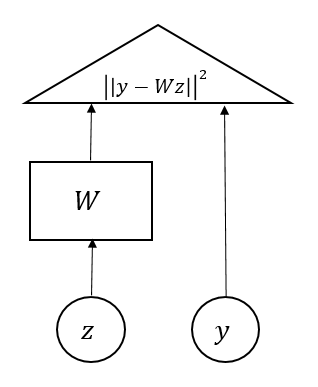
\includegraphics[width=0.35\textwidth]{lectures/10-b/image/pic7.png}
    \caption{The architecture of PCA}
    \label{figure2}
\end{figure}

The architecture for K-means clustering has no encoder, only a decoder and a reconstruction cost module. 
The energy function of K-means is shown in Figure \ref{figure3}, as $y$ moves away from each prototype, the energy goes quadratically. 
The volume that can take low energy is limited by $k$. 
The only points that are reconstructed with zero energy are the prototypes. Every other point has higher energy.

 \begin{figure}[H]
    \centering
    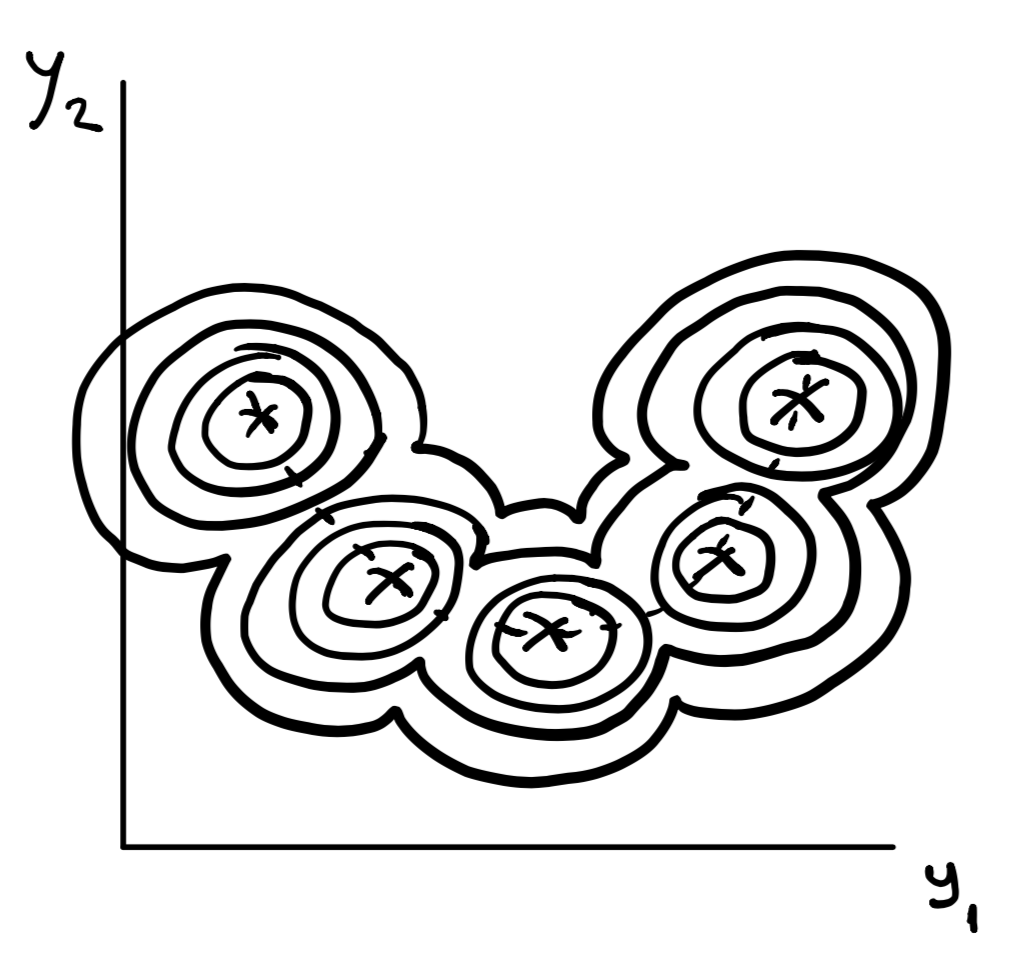
\includegraphics[width=0.5\textwidth]{lectures/10-b/image/pic9.png}
    \caption{Energy function of k-means}
    \label{figure3}
\end{figure}

In Figure \ref{figure4}, the grey level represents energy, dark indicates low energy. 
Use the PCA as example, PCA avoids flat energy surface by using a code with a lower dimension than the input. 
Minimize the distance of every point with the projection, in this example is basically fitting a line to these points. 
The volume that can take low energy in PCA is limited, only a linear subspace of the input can have low energy, everything outside the subspace will have higher energy. 

PCA:
\begin{equation}
E(y,z) =  \norm{W^\top WY -Y}^2
\end{equation}

K-Means
\begin{equation}
E(Y) =  min_z \sum_i\norm{Y-W_iZ_i}^2
\end{equation}

\begin{figure}[H]
    \centering
    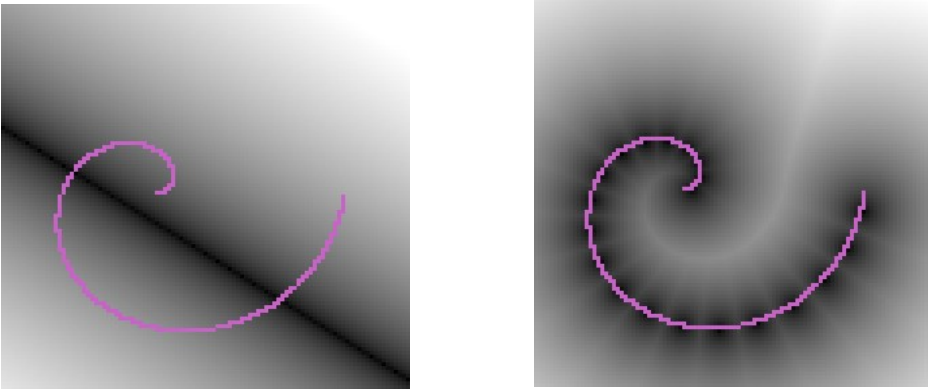
\includegraphics[width=\textwidth]{lectures/10-b/image/pic1.png}
    \caption{Left: PCA and Right: K-Means}
    \label{figure4}
\end{figure}
   
\subsubsection{Push down of the energy of data points, push up everywhere else (Max likelihood (needs tractable partition function))}
    
This what full-fledged probability methods are doing. The probability of a point $y$ is given by Gibbs distribution which is derived from the energy function:
\begin{equation}
    P(Y|W) = \frac{e^{-\beta E(W,Y)}}{\int_y e^{-\beta E(W,y)}}
\end{equation}

Where $\beta$ is an arbitrary positive constant.
Training a probabilistic density model from a training dataset is generally performed by finding the $W$ that maximizes the likelihood of the training data under the model$ \sum^p_{i=1}P(Y^i,W)$. 
Equivalently, we can minimize a loss function $L(W,T)$ that is proportional to the negative log probability of the data. 
Here what we want to do is to minimize the negative log likelihood $L(W,T)$  on the training samples.

\begin{equation}\label{eq177}
    L(W,Y) = \frac{1}{p}\sum^p_{i=1}E(Y^i,W)+\frac{1}{\beta}log\int_y e^{-\beta E(y,W)}
\end{equation}

The gradient of $L(W,T)$ is

\begin{equation}
    \frac{\partial L(W,Y)}{\partial W}= \frac{1}{p}\sum^p_{i=1}\frac{\partial E(Y^i,W)}{\partial W}-\int_y P(y,W)\frac{\partial E(y,W)}{\partial W}
\end{equation}

In other words, minimizing the first term in equation \ref{eq177} with respect to $W$ has  the effect of making the energy of observed data points as small as possible, while minimizing the second term has the effect of “pulling up” on the energy of unobserved data points to make it as high as possible, particularly if their energy is low (their probability
under the model is high).

Naturally, evaluating the derivative of the second term in equation \ref{eq177}  may be intractable when Y is a high dimensional variable and $E(Y, W)$ is a complicated function for which the integral has no analytic solution. 
The intractable integral is often evaluated through:

\begin{itemize}
    \item Monte-Carlo sampling, where we are going to replace the integral with discrete sum, where we draw samples from the distribution and then compute the average of the samples.
    \item Variational approximations, where we replace the distribution $P$ with one that we know how to compute, like Gaussian. 
    So we pick Gaussian which is possible the best approximation to $P$, in terms of KL Divergence, which measures the divergence between distributions. 
    We replace P by Q, and then compute $(17.8)$, while minimizing the divergence between P and Q at the same time.
\end{itemize}

\subsubsection{Push down of the energy of data points, push up on chosen locations (contrastive divergence, Ratio Matching, Noise Contrastive Estimation, Minimum Probability Flow)}

Monte Carlo methods, adversarial training, generative adversarial networks and many more falls under this category.
 
\subsubsection{Minimize the gradient and maximize the curvature around data points (score matching)}

The idea is to take the energy function and try to make it flat around data points.
In other words, we want the gradient of the energy function in $y$ space (with respect to input $y$) to be $0$, because we want the energy to be minimum. 
See figure \ref{figure8} . 
The ideal energy function is the one that take low values around the points and value increases as we move away. 
In other words we can define score matching as having an energy function that has zero gradient with respect to the input, while also having a second derivative that is as large as possible. 
However, the problem is that we have to compute the gradient of the trace of the Hessian with respect to the parameters. 
This idea is \textit{"cute but impractical"}, except for very simple models. 

\begin{figure}[htb]
    \centering
    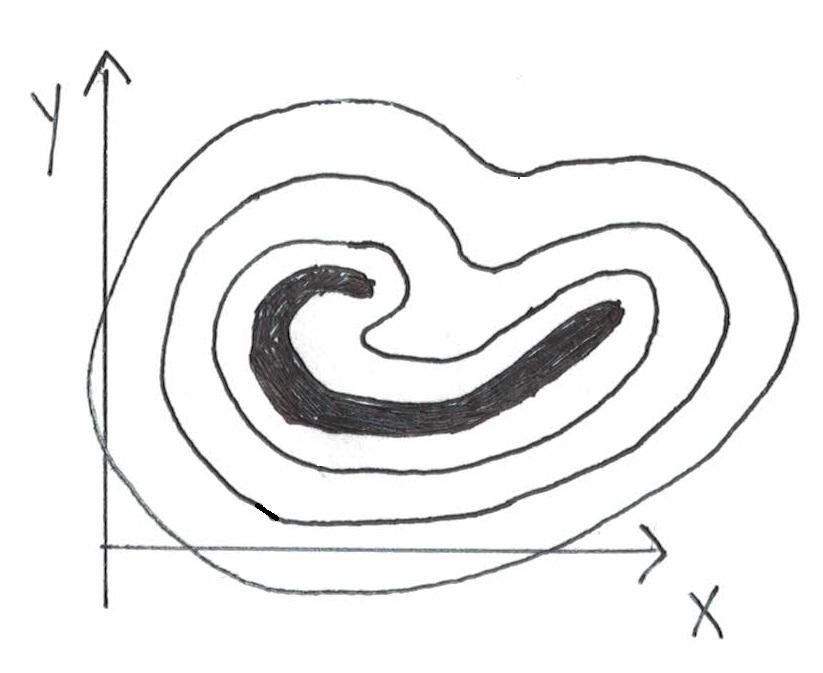
\includegraphics[width=0.35\textwidth]{lectures/10-b/image/pic8.png}
    \caption{Energy Function}
    \label{figure8}
\end{figure}

\subsubsection{Train a dynamical system so that the dynamics goes to the manifold (denoising auto-encoder)}

The idea of denoising auto-encoder is very useful. 
We start with the raw input $y$, and corrupt it with some noise, and then run it through some parameterized function $G_w(y)$. 
Then we take the uncorrupted input and compute the distance with the output from the function $G_w(y)$. 
By applying corruption and function $G_w(y)$, we are supposed to reconstruct the original $y$ with its prediction $\bar y$. 
Then we minimize the reconstruction error, which is the square of distance between $\bar y$ and $y$.
See \ref{figure6}. 
In other words, the function $G_w(y)$ maps the point outside the manifold to the point inside the manifold. 
At test time, we remove the corrupt part and give a $y$ without corruption. 

The energy-based view of denosing auto-encoder is that when we train the function to map the points outside the manifold to the points on the manifold, we train it to compute the energy, which is the reconstruction error.

Two slight problems remain:

\begin{itemize}
    \item We don't know what noise, or what types of corruptions make sense.
    \item There are many ways that one can corrupt an input in the high dimensional space.
    We may not be able to cover all possible ways to corrupt an input that can span the high dimensional space. 
    Besides, there is no guarantee that the model learns exactly what we teach it. It may not be able transform all the points to the manifold.
\end{itemize}

\begin{figure}[htb]
    \centering
    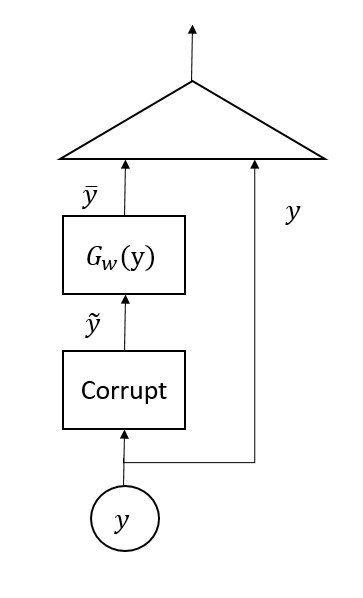
\includegraphics[width=0.35\textwidth]{lectures/10-b/image/PIC6.PNG}
    \caption{The architecture of denoising auto-encoder}
    \label{figure6}
\end{figure}

\subsubsection{Use a regularizer that limits the volume of space that has low energy}
This will be discussed in more detail on April 29.
    
\subsubsection{If $E(Y) = ||Y - G(Y)||^2$, make $G(Y)$ as "constant" as possible.(Contracting auto-encoder, saturating auto-encoder)}

Contracting auto-encoder comes from Yoshua Bengio's lab. Basically, it's still in the architecture of auto-encoder in figure  \ref{figure5}.

\begin{figure}[htb]
    \centering
    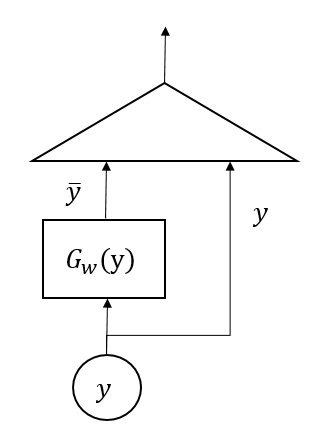
\includegraphics[width=0.35\textwidth]{lectures/10-b/image/PIC5.PNG}
    \caption{The architecture of auto-encoder}
    \label{figure5}
\end{figure}

The energy of $y$ is $$ E(y) = ||y-G(y)||^2, $$ and the loss function is $$L = \sum_i E(y^i)+R(w),$$ where the regularization term $R(w)$ is the square Frobenius norm of Jacobian of the hidden layer representation with respect to input values. 
This encourages a constant hidden representation except around training samples where it is counteracted by the reconstruction term.
\chapter{The Truck Backer-Upper}
% Authors: Xiao Jing, Arnav Kansal, Changgeng Zhao, 4/30/19.

\section{Set up}
We try to design a self-learning nonlinear controller to control the steering of a trailer truck while backing up a loading dock from an arbitrary initial position. Only backing up is allowed to park the truck parallel to the dock and trying to match ($x_{trailer}$, $y_{trailer}$) with ($x_{dock}$, $y_{dock}$) as closely as possible. In the lecture, some students tried to play this game and we found it's very hard even for humans to accomplish the task.
\\
\begin{figure}[H]
    \centering
    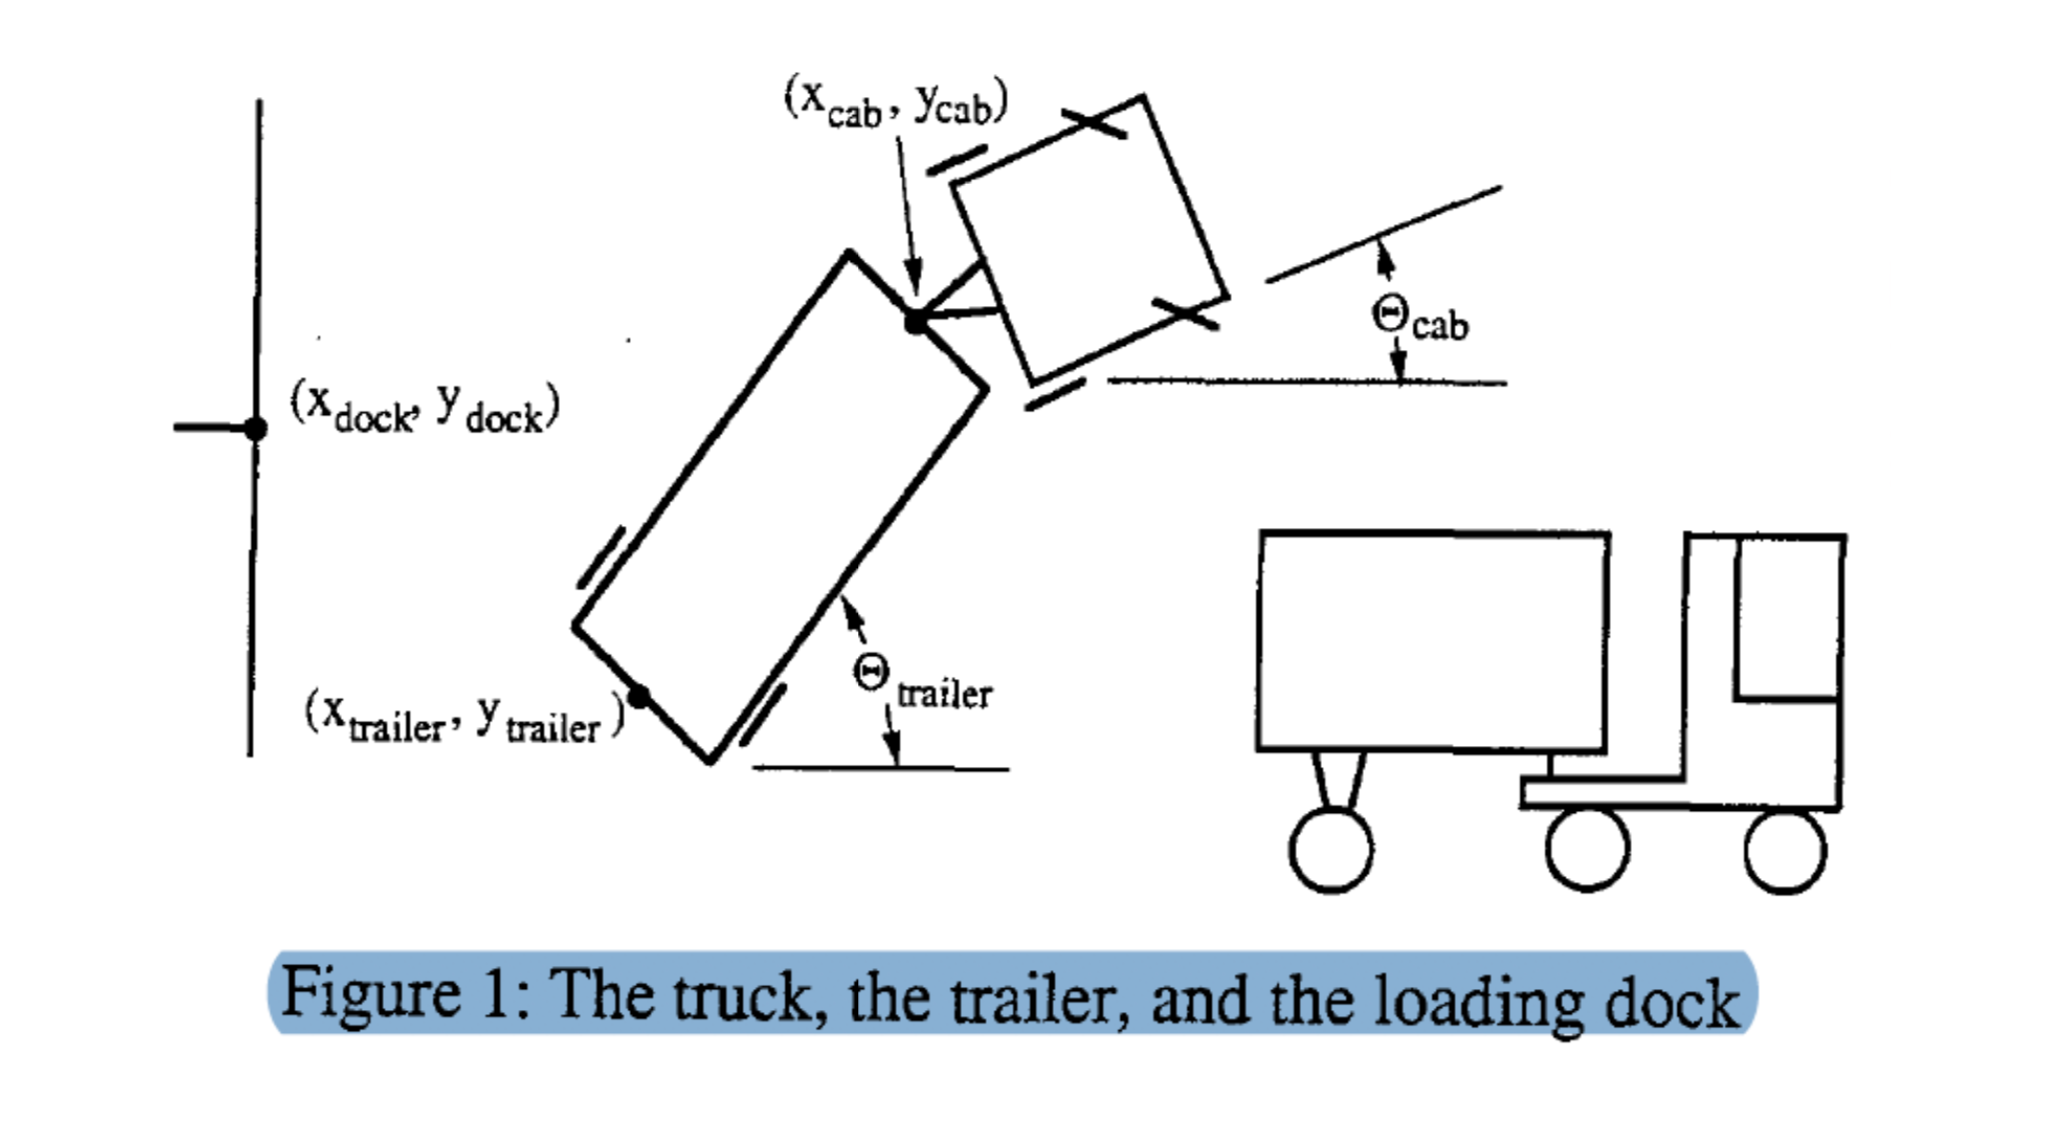
\includegraphics[width=0.7\textwidth]{figs/truck-trailer-and-loading-dock.png}
    \caption{The Truck, trailer and loading dock}
    \label{fig:general}
\end{figure}
State variables representing the position of the truck: $\theta_{cab}$, the angle of the truck, $x_{cab}$ and $y_{cab}$, the cartesian position of the yoke, $x_{trailer}$ and $y_{trailer}$, the cartesian position of the rear of the center of the trailer, $\theta_{trailer}$, the angle of the trailer.

\section{Model and two stage learning}
\subsection{Model}
\begin{figure}[H]
    \centering
    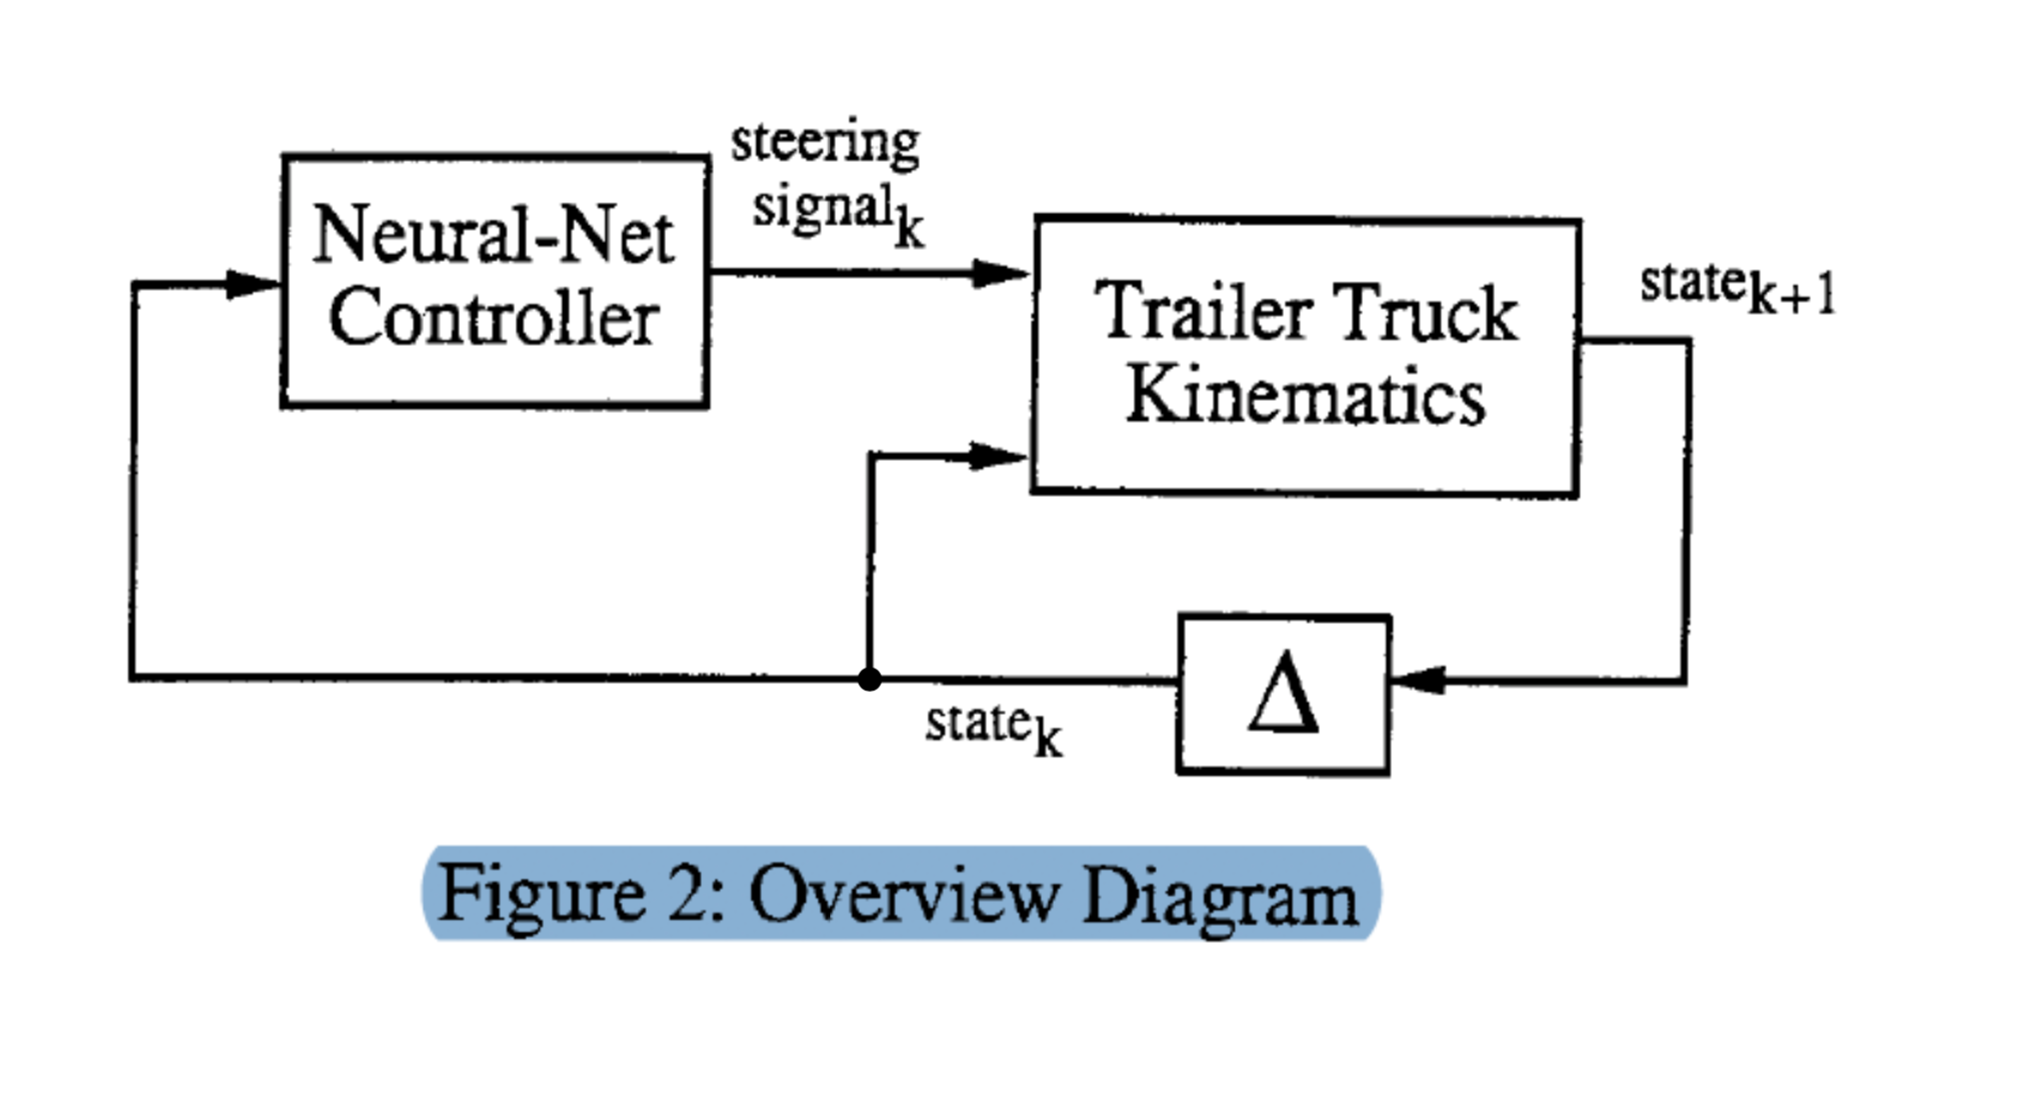
\includegraphics[width=0.6\textwidth]{figs/the-two-part-model.png}
    \caption{The two part model}
    \label{fig:learn}
\end{figure}
The proposed model has two elements: the \textbf{Kinematics Component} (emulator) and the \textbf{Neural Net Controller}. The trailer truck Kinematics Component of the model tries to learn the next state of the truck given the current state and the steering action. The Neural Net Controller learns the steering action given the current state of the truck. We train the two models separately: first train the Kinematics Component and then based on this model we train the Controller by back-prop through Kinematics model.


 
\subsection{Variable Input}
In the paper, there are 6 parameters. However, we just need 4 variables in state $k$, which are shown in the next slide, since cab coordinate can be calculated according to the four values we have.
\begin{figure}[H]
    \centering
    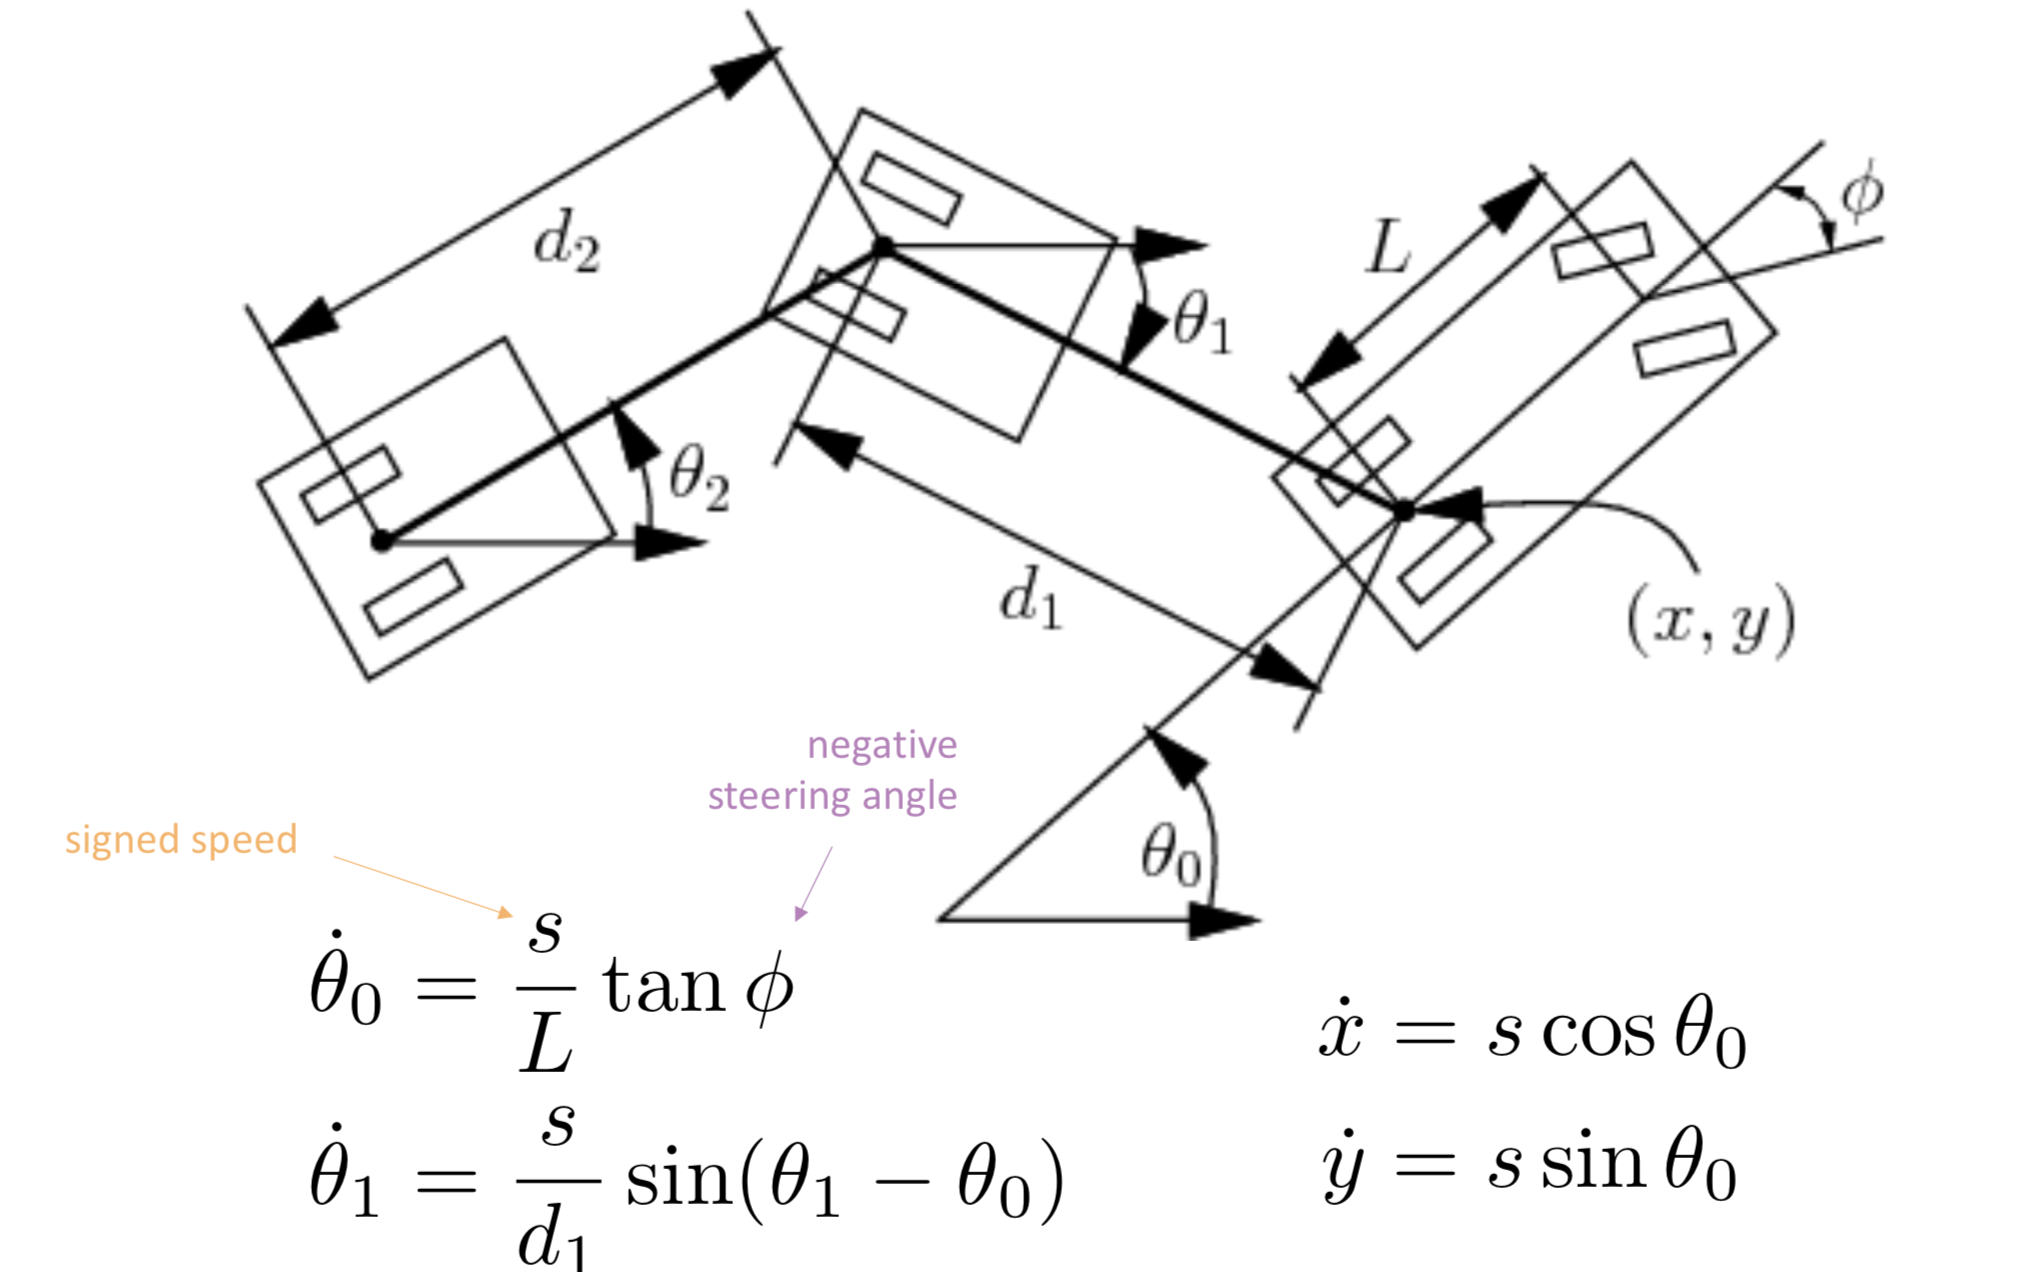
\includegraphics[width=0.6\textwidth]{figs/variable.png}
    \caption{Variable}
    \label{fig:variable}
\end{figure}

\subsection{Flow chart}
The block labeled $C$ represent the controller and $T$ represent the emulator. The initial position of truck is chosen at random. The final error is used by back-propagation to adapt to each state Controller/Trailer.
\begin{figure}[H]
    \centering
    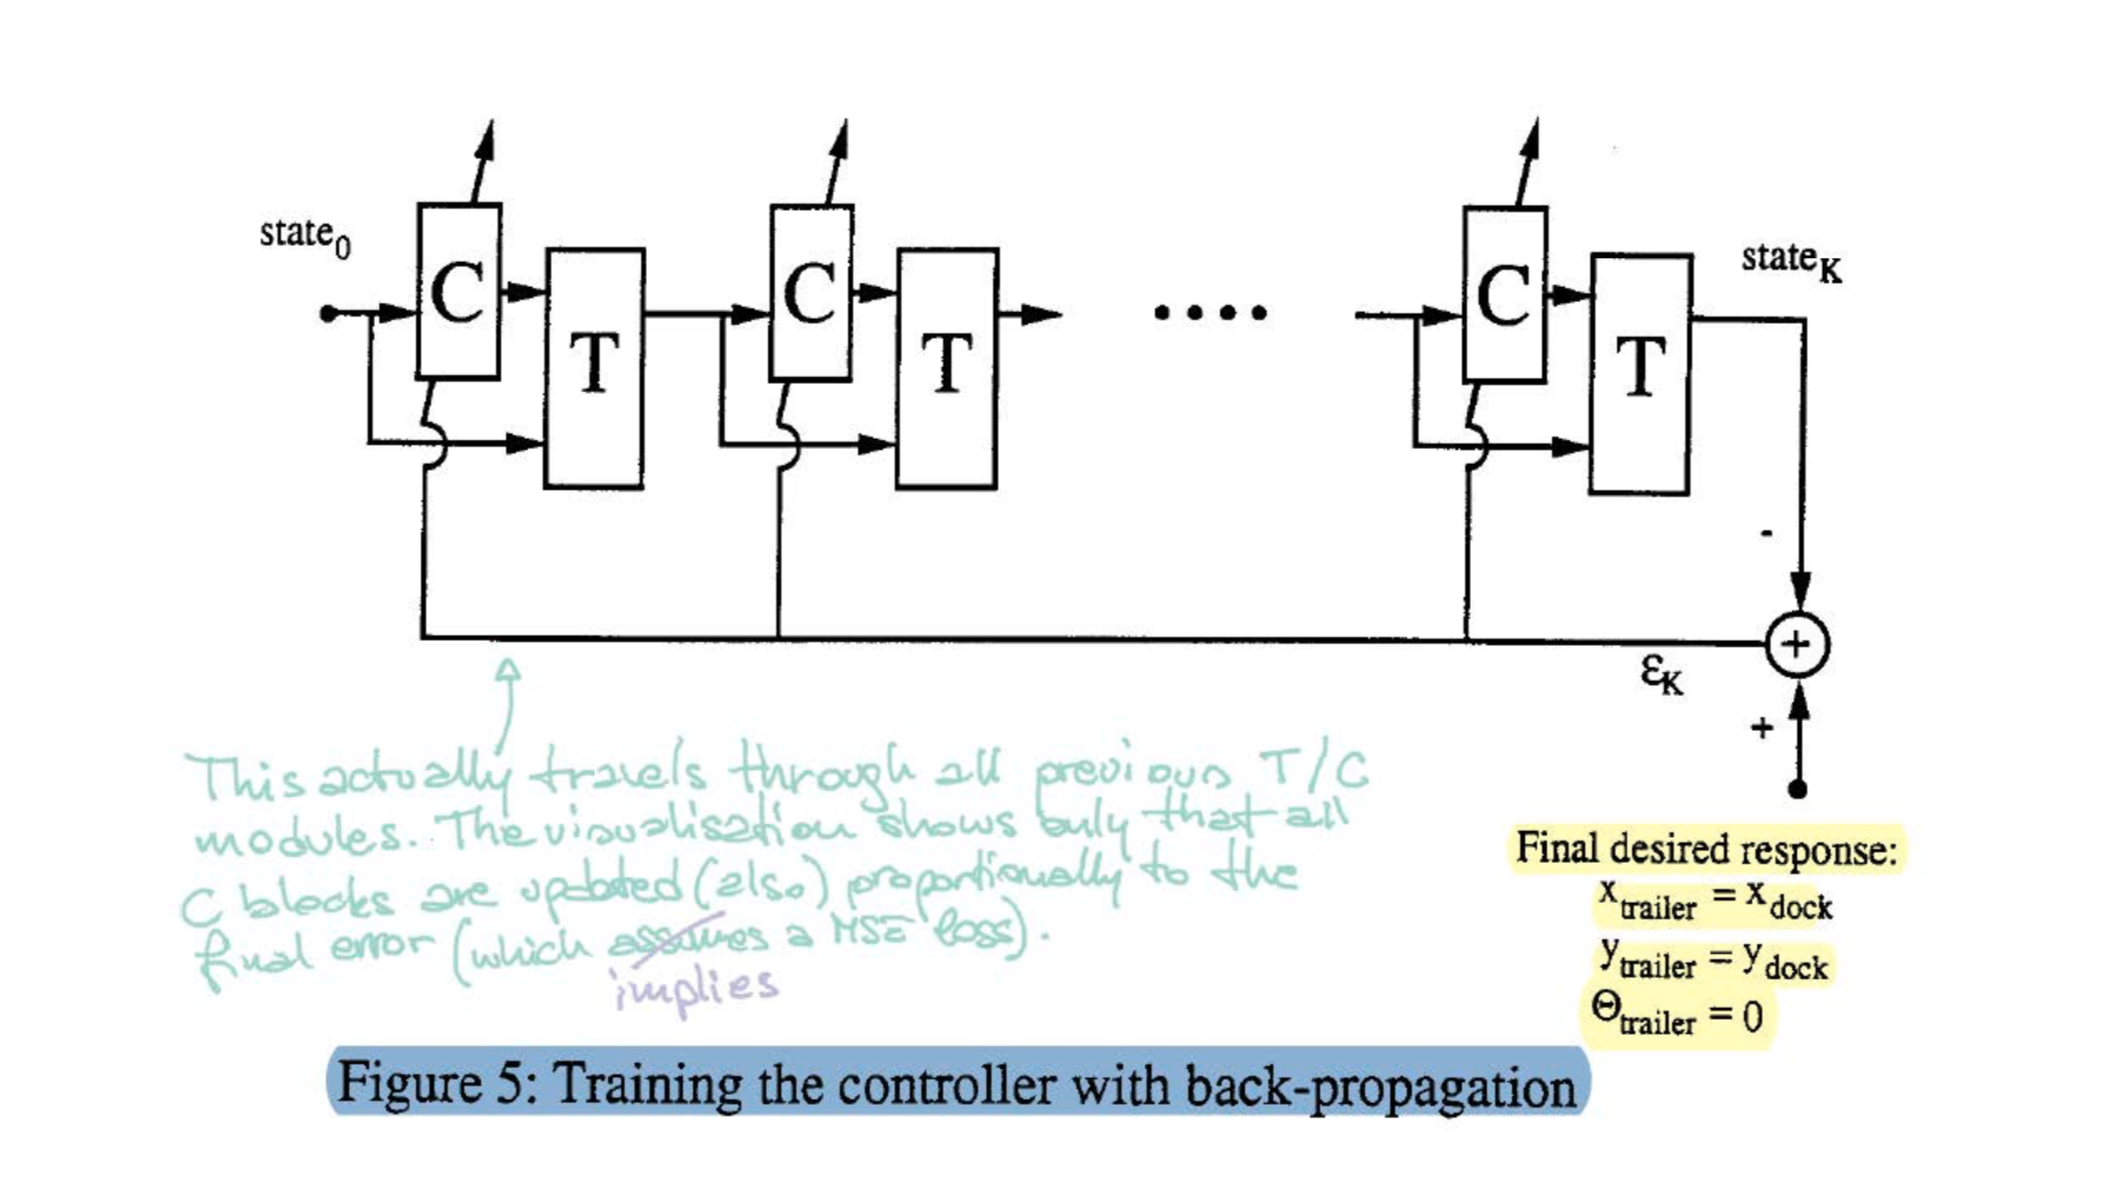
\includegraphics[width=0.8\textwidth]{figs/training-the-controller.png}
    \label{fig:loss}
\end{figure}
Each time, we have 6 inputs for controller at state $k$, and we add bias and forward the inputs to 25 hidden units, and give 1 output unit. So there are 3 layers in the controller. 
\\
Then we put the controller's output to the Emulator, which has 45 hidden units and 6 output for the next state. It is analogous to a neural network having a number of layers equal to four times the number of backing up steps.
\begin{figure}[H]
    \centering
    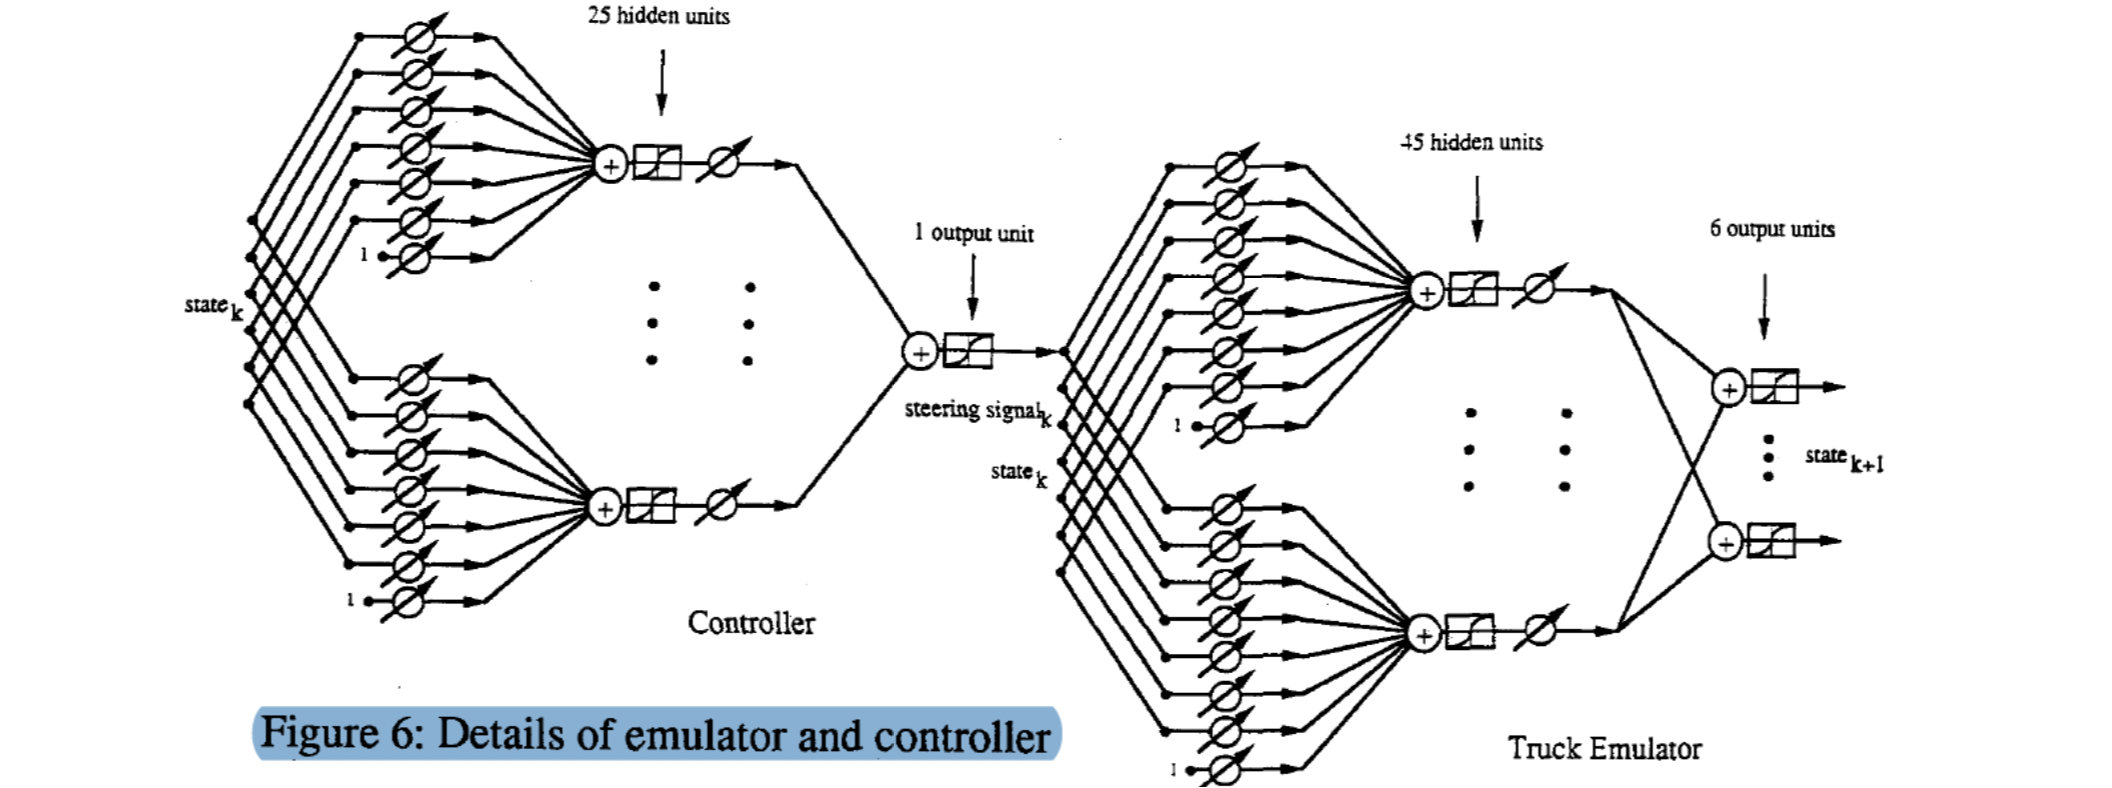
\includegraphics[width=0.8\textwidth]{figs/details-of-emulator.png}
    \label{fig:nn}
\end{figure}

\subsection{Loss Function}
Here the $\theta_c$ is $\theta_0$, the $\theta_t$ is $\theta_1$

\begin{equation*}
    ||\theta_{t}||^2 + ||(x_{\text{trailer}}, y_{\text{trailer}}) - (x_{\text{dock}}, y_{\text{dock}})||^2     
\end{equation*}

% \begin{figure}[H]
%     \centering
%     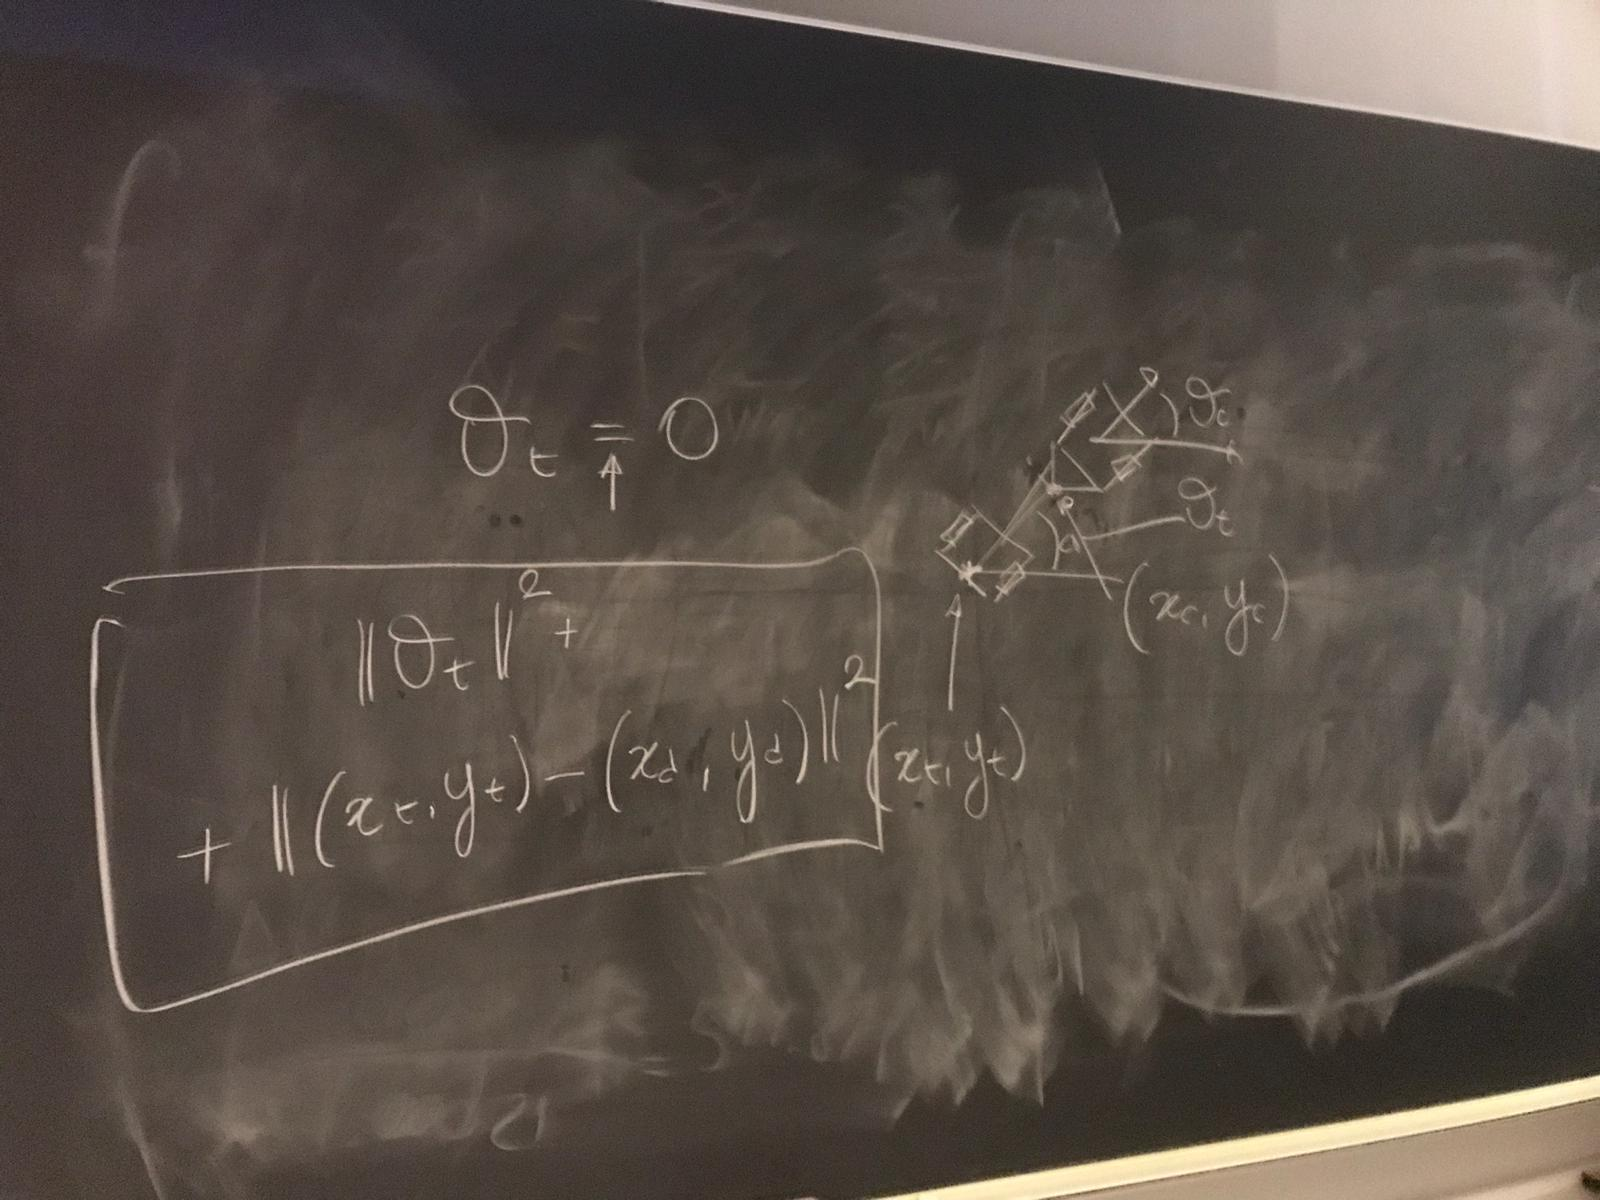
\includegraphics[width=0.7\textwidth]{labs/13/images/loss.jpeg}
%     \caption{loss}
%     \label{fig:loss}
% \end{figure}



\subsection{Two stage Learning}\label{sec:truck-model}
In the first stage of learning, the emulator is fed as input : states of the truck along with random steering actions and the actual state of the truck (according to the physics of the system) as output to learn. The emulator can then predict the next state of the truck given an initial state and the steering action.

The second stage of learning involves unrolling the controller for the length of the actions of the episode and recursively applying the controller to the states produced by the action the controller takes. This produces a final state of the truck which is used to calculate the loss and used to update the parameters of the controller via back propagation through time.

\begin{itemize}
\item Q: Why don't we use the kinematics equations directly as we already know how a track move? 
-- A: Because we want to show that the model can learn the kinematics facts automatically, which is useful in other complicated scenarios where we can not know how it works.
\end{itemize}

\subsection{Initial to final state}
Traces of trajectory guided by the learned system in action.
\begin{figure}[H]
    \centering
    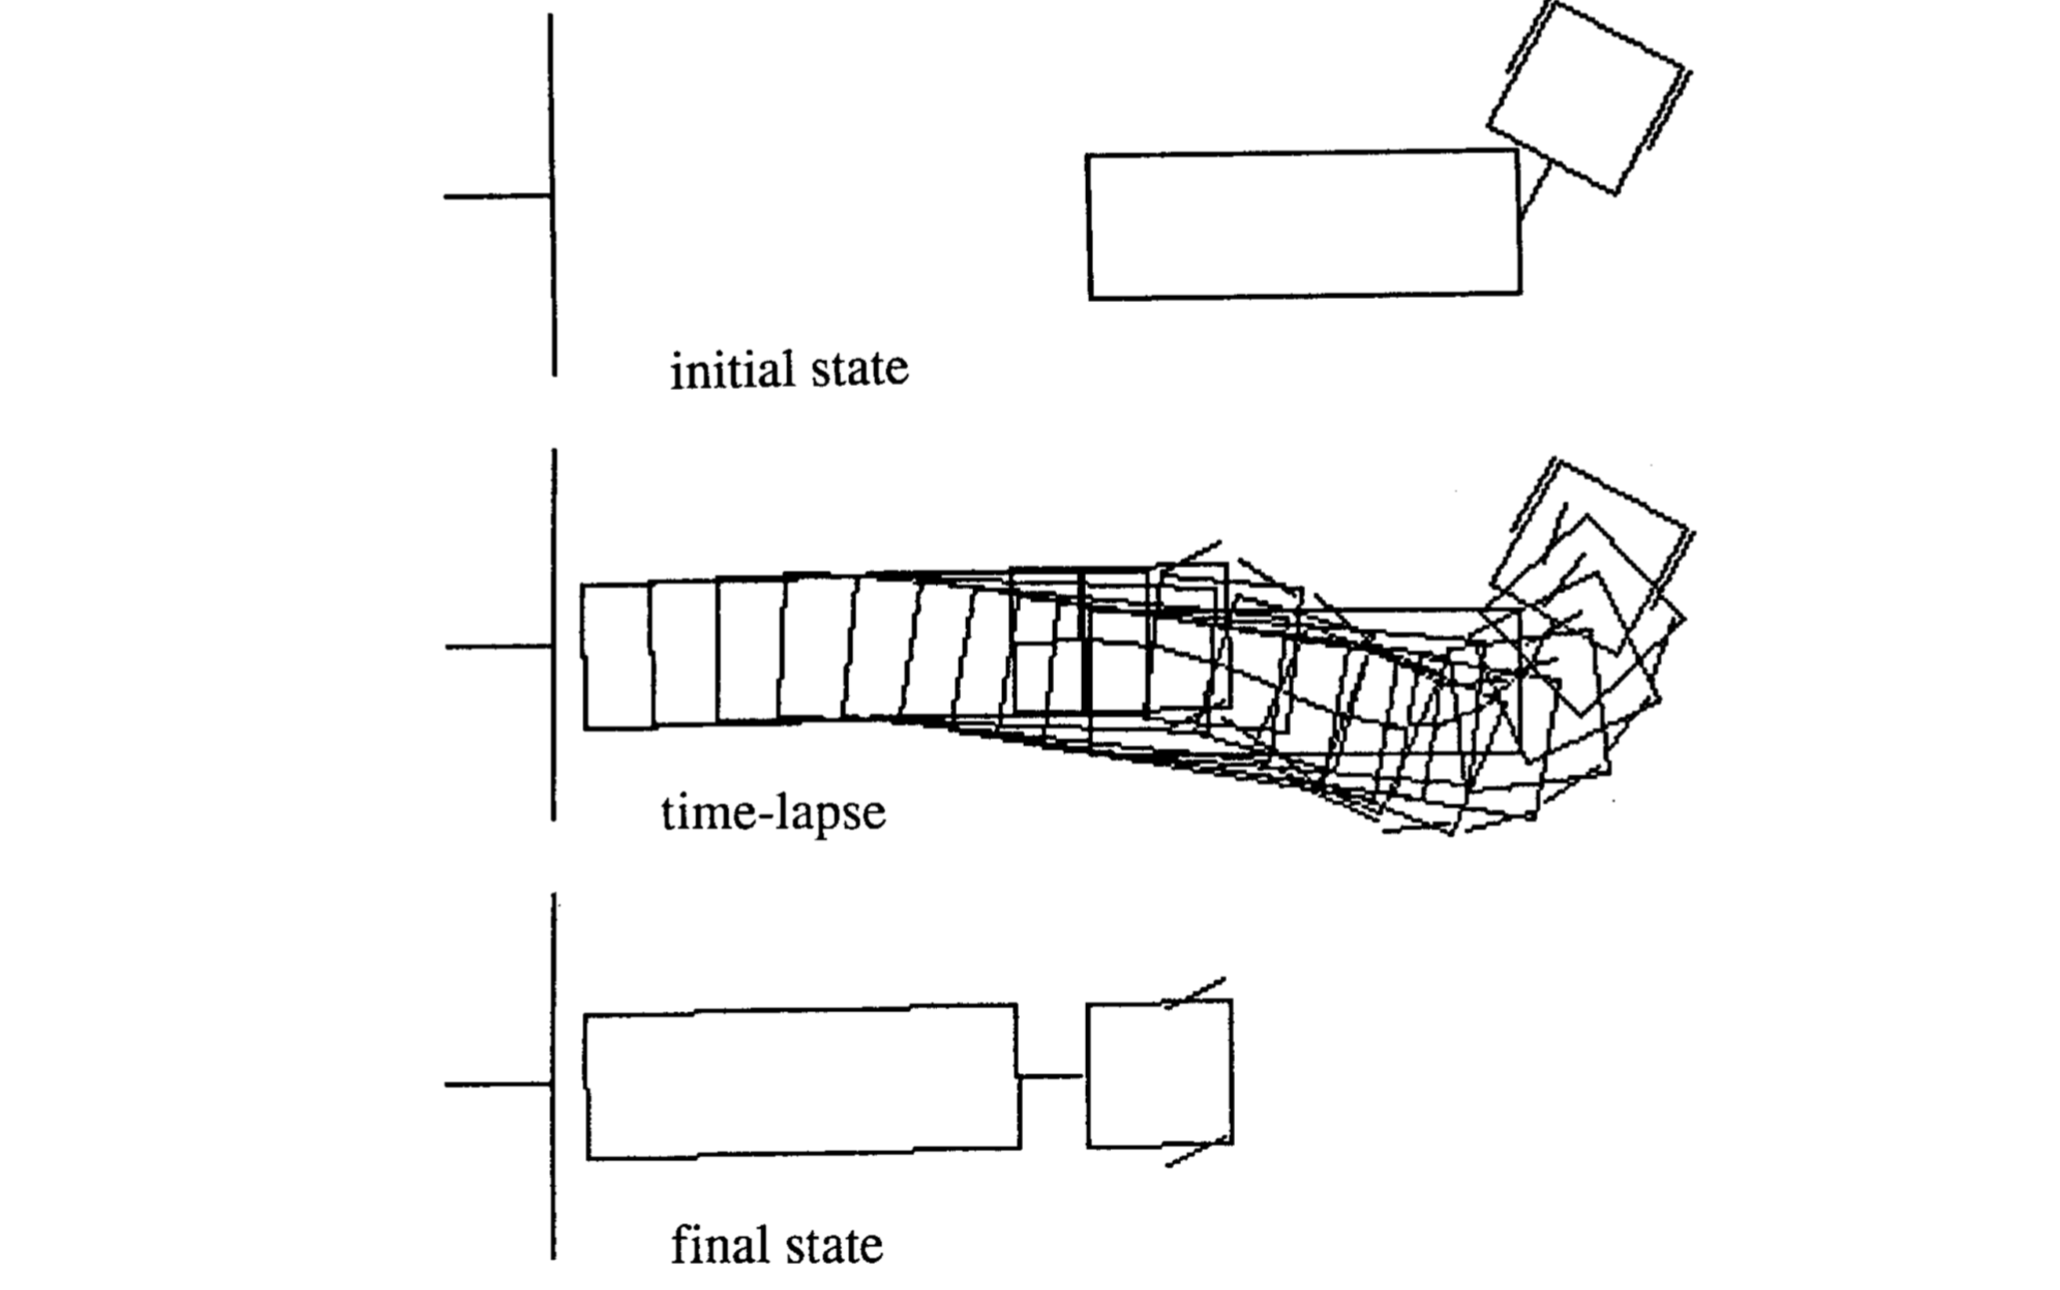
\includegraphics[width=0.45\textwidth]{figs/state.png}
    \label{fig:state}
    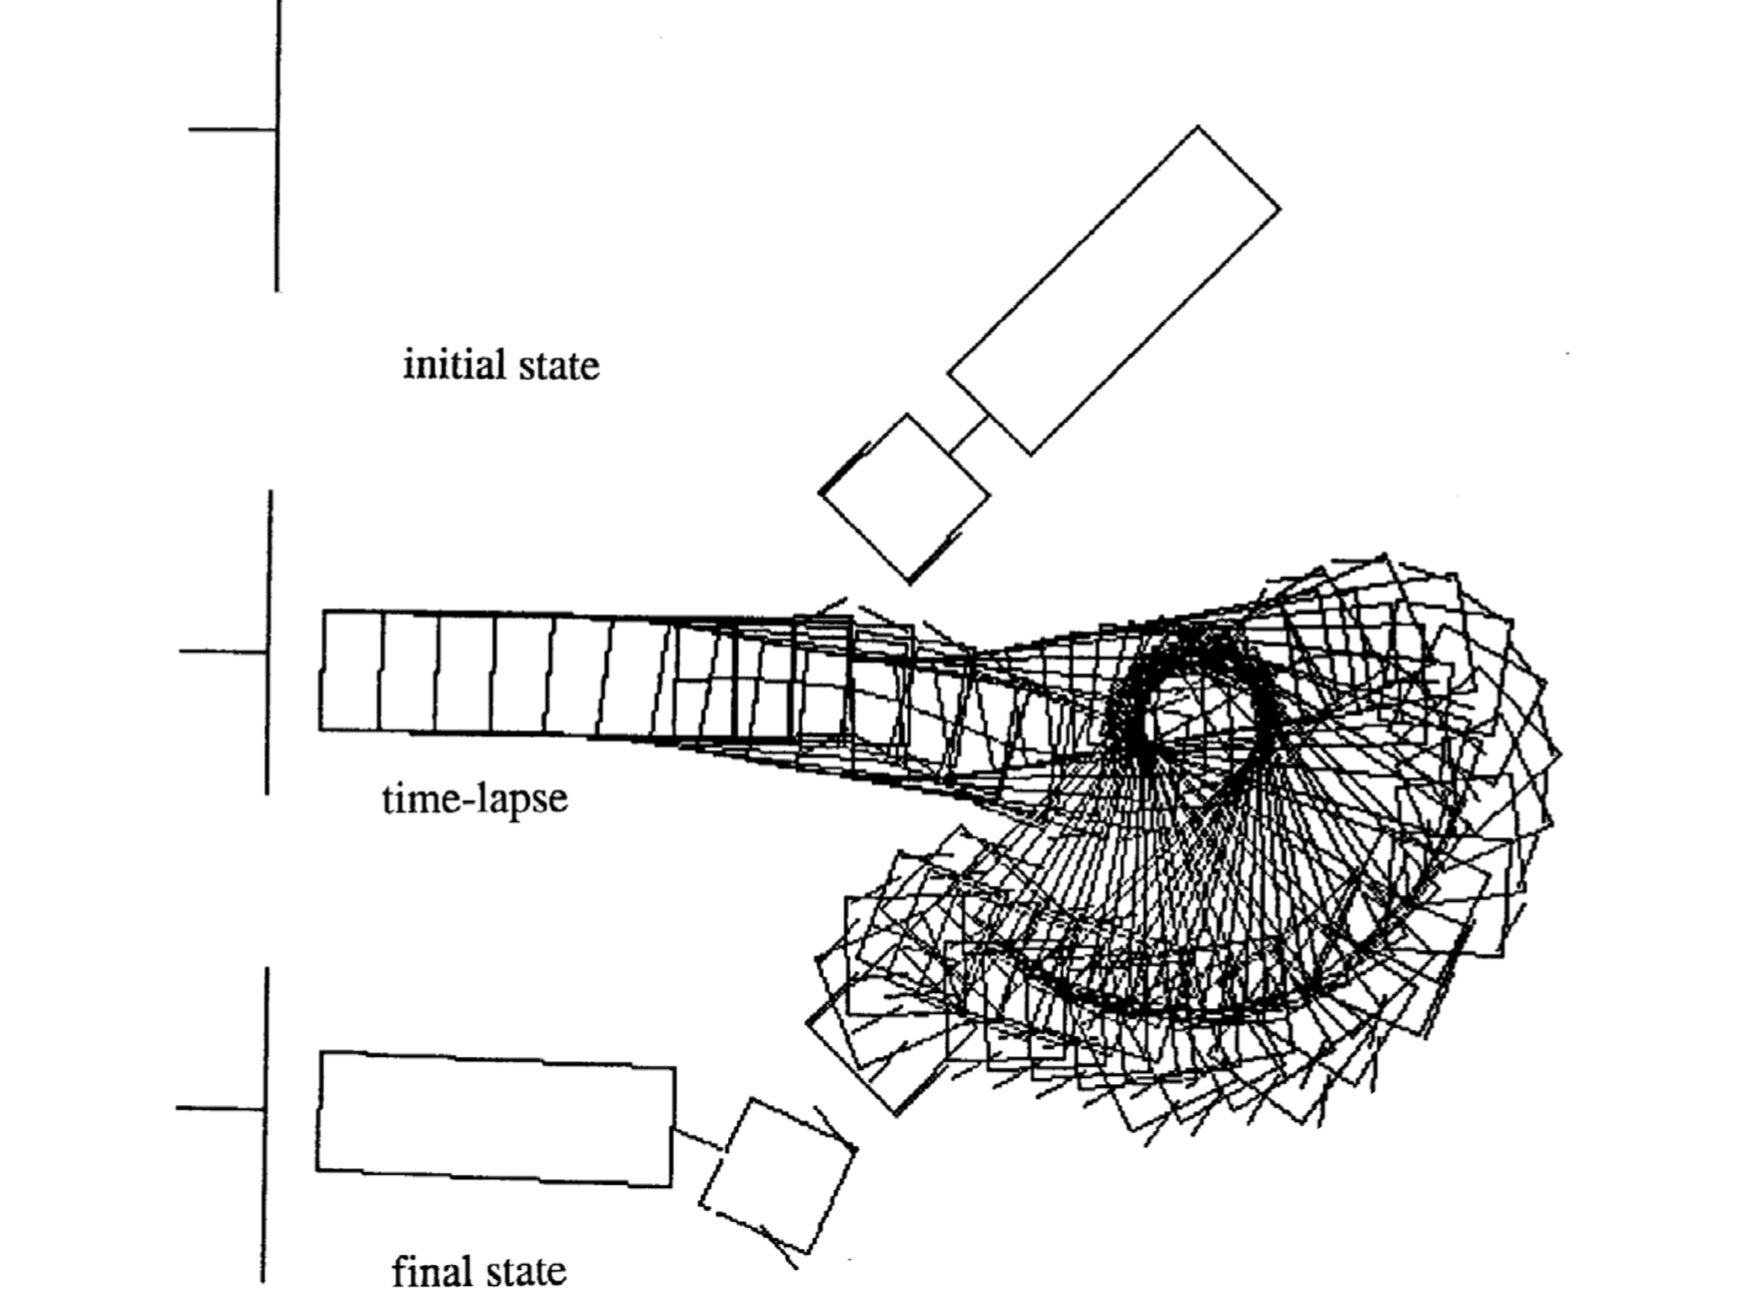
\includegraphics[width=0.45\textwidth]{figs/state2.png}
    \label{fig:state2}
\end{figure}
%%%%%%%%%%%%%%%%%%%%%%%%%%%%%%%%%%%%%%%%%%
\part{Architectures}\label{prt:arch}
%%%%%%%%%%%%%%%%%%%%%%%%%%%%%%%%%%%%%%%%%%
\chapter{Components of a CNN}
% Authors: Joanna Bitton, Divyansh Khanna, Lind Xiao, 2/26/19.

\section{Variety of layers}
% Authors: Joanna Bitton, Divyansh Khanna, Lind Xiao, 2/26/19.
A convolutional neural network may consist of various kinds of layers.
Each layer is responsible for extracting relevant information and creating higher-level interpretations of the input.
In a standard CNN, an input will go through a series of layers such as convolution, non-linearity, pooling, and batch normalization layers.

\subsection{Convolution}
% Authors: Joanna Bitton, Divyansh Khanna, Lind Xiao, 2/26/19.
A convolution layer is the backbone of all convolutional neural networks.
The layer contains a set of learnable filters that will produce an activation map displaying how the input has responded to each filter.
For instance, a filter could attempt to detect a certain kind of edge present in the input, or in higher levels of the network detect a shape.
This is achieved by using small spatial filters that convolve over the height and width of the image, computing the dot product at every position.
The output of each filter will produce a two-dimensional activation map which will be stacked along the depth-dimension to create the output for the layer.

\subsection{Non-linearity}
% Authors: Joanna Bitton, Divyansh Khanna, Lind Xiao, 2/26/19.
Without a non-linearity module present in the network, no matter how many layers are defined, the neural network would behave like a single-layered model. 
This is due to the fact that summing these layers would simply output another linear function.
Additionally, with the inclusion of non-linearity modules, non-linearity is introduced into the model and thus more complex concepts can be learned.
The ReLU activation function is typically used as opposed to hyperbolic tangent as it is faster to train.
Despite the theoretical need for nonlinearities to be added, there is a paper that was able to train a deep model without nonlinearity layers.
Interestingly enough, the floating point approximations from the calculations were enough of a nonlinearity to train the model.

\subsection{Pooling}
% Authors: Joanna Bitton, Divyansh Khanna, Lind Xiao, 2/26/19.
Downsampling the input is an important component of learning representations with a CNN.
A pooling layer after a convolution layer is used to progressively downsample the spatial size of the representation.
Thus, the amount of parameters and computation in the network is reduced.
This helps in preventing overfitting.
Additionally, a pooling layer is essential in establishing translation invariance.
An edge detected at one corner of the image will still be an edge when picked up at a different part of the image (and possibly rotated as well).
Max-pooling will let the network preserve this edge despite losing its location.

In practice, using $2\times 2$ pooling with a stride of 2 for instance, 75 percent of the information will be lost.
Since much of the information is lost, it is generally a rule of thumb that the depth of the feature map is doubled using a convolutional layer beforehand.
Then, the pooling is performed with only a 50 percent information loss instead.

\subsection{Batch normalization}
% Authors: Joanna Bitton, Divyansh Khanna, Lind Xiao, 2/26/19.
The batch normalization layer is typically invoked after a non-linearity.
$$
\begin{aligned}
\mu_B & =\frac{1}{m} \sum_{i}^m x_i\\
\sigma_B & = \frac{1}{m}\sum_i^m (x_i-\mu_B)^2\\
\hat{x}_i & = \frac{x_i -\mu_B}{\sqrt{\sigma_B +\epsilon}}
\end{aligned}
$$

Batch normalization is a commonly used trick to speed up training performance in convolutional neural networks, while providing robustness to the network.
A batch normalization layer normalizes the data in each batch to have zero mean and unit variance.
It provides the ability to decouple subsequent layers such that the current layer does not have to keep track of the moving statistics of the previous layers.
If batch normalization is not applied, every time a weight is changed in the lower layers everything propagates up and there is too much interaction between the upper and lower layers.
It also provides some consistency between layers by reducing internal covariate shift (\href{https://arxiv.org/abs/1502.03167}{paper}).

\section{Residual Connections}
% Authors: Joanna Bitton, Divyansh Khanna, Lind Xiao, 2/26/19.
An important problem with training deeper neural networks has been the loss of gradients as deeper parts of the network are approached.
This is commonly referred to as the \textbf{vanishing gradient problem}.
One way the deep learning community has been able to overcome this issue is by using residual connections in the neural network (\href{https://arxiv.org/abs/1512.03385}{paper}).
A residual connection (or skip connection) connects an output of a layer to another layer by jumping over layers.
The weights of the skip connections are learned as the network learns.
By skipping over layers, the network is able to propagate gradients and ensure better representation learning.
General construction looks like:
$$
\begin{aligned}
y_k & = h(x_k) +\mathcal{F}(x_k, \mathcal{W}_k)\\
x_{k+1} & = f(y_k),
\end{aligned}
$$
where $h(x_k)$ is the bypass short cut and $h(\_)$ is commonly taken to be identity map.

There are a decent amount of variants proposed in the research community which are based on skip connections.
DenseNets (\href{https://arxiv.org/abs/1608.06993}{paper}) has several parallel skip connections within each block.

Figure 1 (\href{https://arxiv.org/pdf/1712.09913.pdf}{original paper}) depicts how the use of residual connections makes the loss landscape smooth, which allows the network to converge.

\begin{figure}
    \centering
    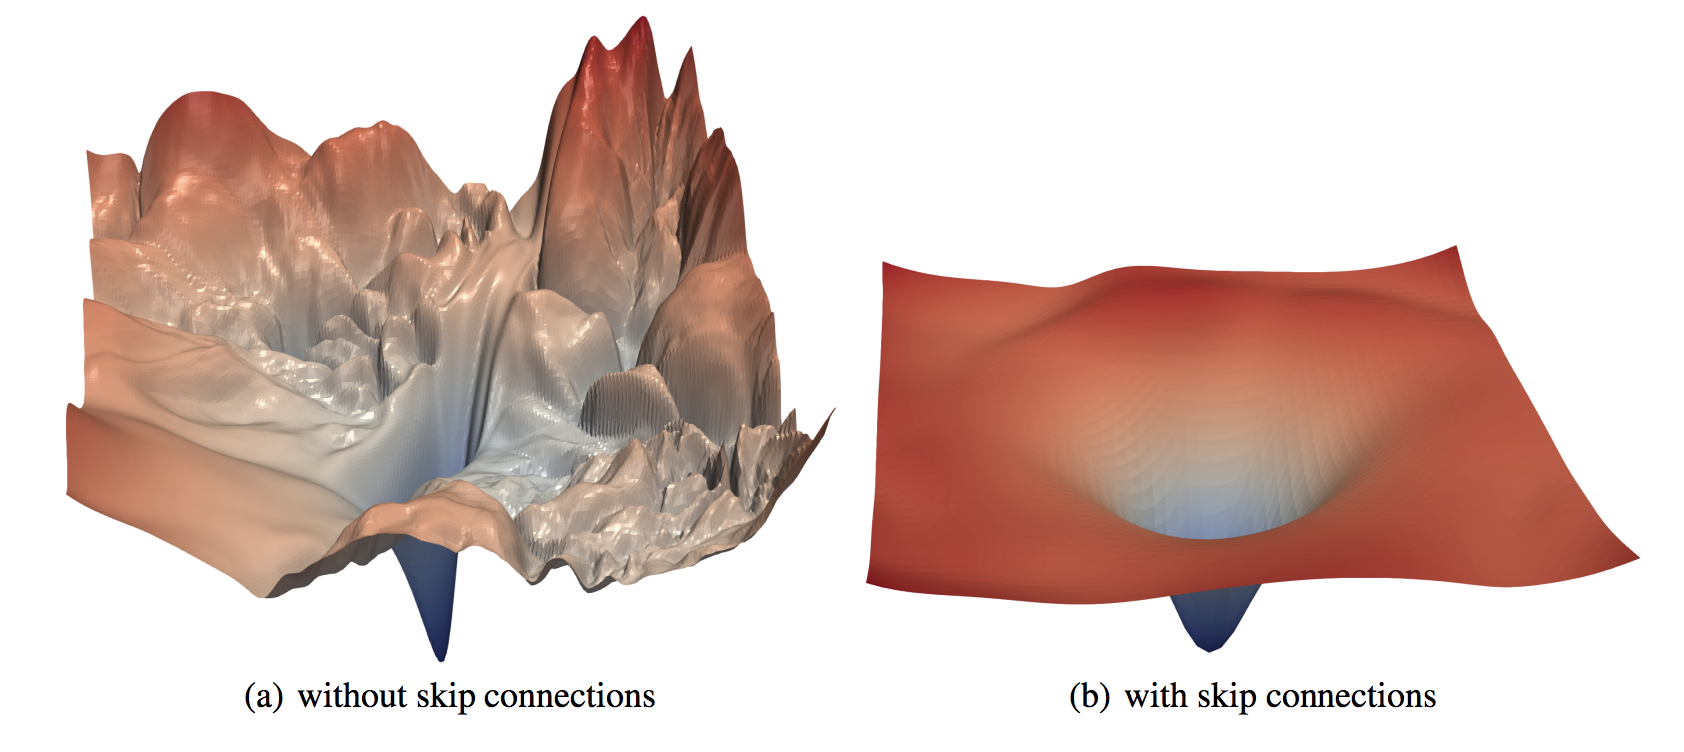
\includegraphics[width=\textwidth]{figs/loss.png}
    \caption{ The loss surfaces of ResNet-56 with/without skip connections.}
    \label{fig:my_label0}
\end{figure}

\section{Information Bottleneck}
% Authors: Joanna Bitton, Divyansh Khanna, Lind Xiao, 2/26/19.
As information moves up the layers, it passes through different layers which filter out relevant features.
This commonly requires altering the dimensions of the information.
For example, recall that one reason pooling is used is to reduce the size of the feature maps.
This dimensionality reduction plays an important role in how the network learns.
The method of extracting relevant information and forgetting the rest is known as a procedure called ``Information Bottleneck".
There has been an increasing interest in the information theory aspect of how deep neural networks work, and how the architectures help them generalize well (\href{https://openreview.net/forum?id=ry_WPG-A-}{paper}). %components of cnn
\chapter{Recurrent Nets}
% Authors: Qintai Liu
% Lecture date: 3/11/2019

\section{Simple Recurrent Net}
\label{sec:SimpleRecNet}
% Authors: Qintai Liu
% Lecture date: 3/11/2019

RNN is designed to capture sequential information.
Some of the inputs of traditional neural network are independent of each other.
But in many tasks, the inputs are actually dependent of each other.
In order to predict what the next word is in a sentence, you better know which words appear before it.
Recurrent nets perform the same task for every element of a sequence, with the output being depended on the previous computations. 
RNNs can take advantage of information in arbitrarily long sequences theoretically, but in reality they are limited to capturing long-term dependencies.
Here is what a typical RNN looks like:\cref{fig:Simple RNN}

\begin{figure}[h]
    \centering
    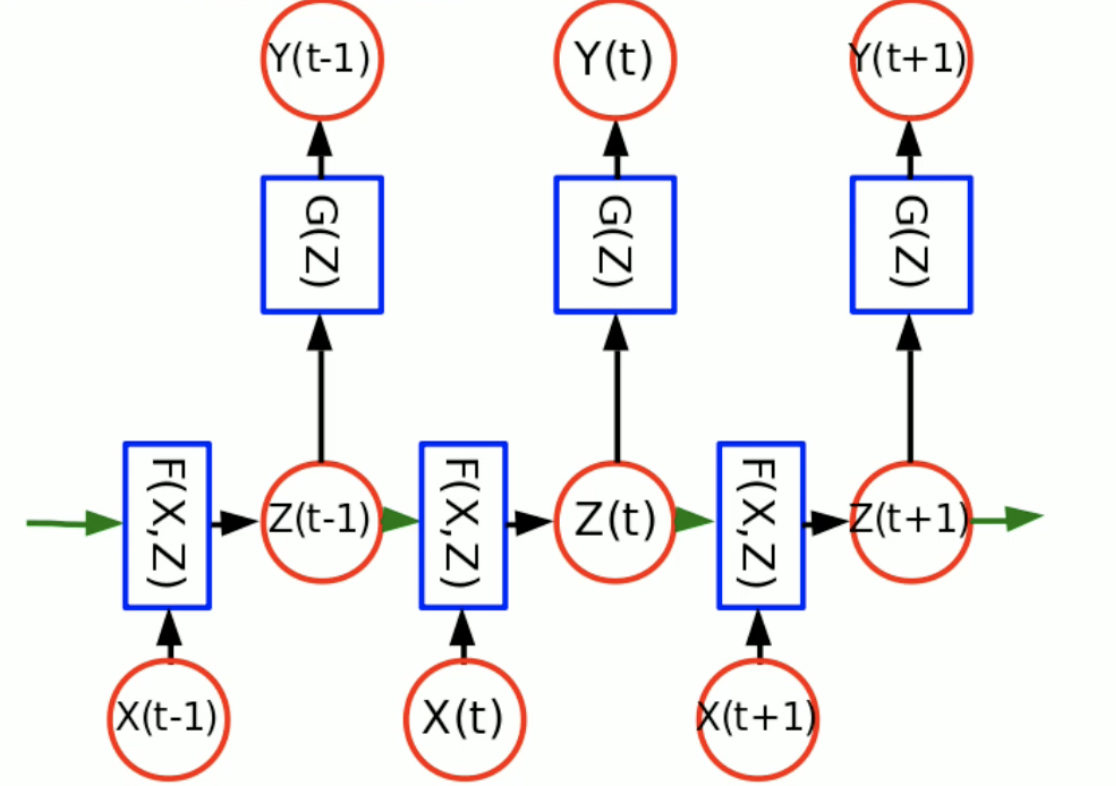
\includegraphics[width=150pt]{figs/image/rnn.png}
    \caption{Simple Recurrent Net}
    \label{fig:Simple RNN}
\end{figure}

\begin{itemize}
  \item $\vect{x_{t}}$ is the input at time step $t$
  \item $\vect{z_{t}}$ is the hidden state at time $t$. $\vect{z_{t}}$ is calculated based on the input at the current step and the previous hidden state:
  $\vect{z_t} = F(\vect{x_t}, \vect{z_{t-1}})$
  \item $\vect{y_t}$ is the output at step $t$. $\vect{y_t} = G(\vect{z_t})$
\end{itemize}



\section{Issue of Simple Recurrent Net}
% Authors: Qintai Liu
% Lecture date: 3/11/2019
\subsection{Backpropagation Through Time}
% Authors: Qintai Liu
% Lecture date: 3/11/2019
In order to know the issue of simple RNN, we first need to know how the gradient is calculated in terms of RNN. Suppose the hidden state($\vect{z_t}$) is calculated as below:

\[\vect{\bar{z_t}} = \matr{W_X} \vect{x_t} + \matr{W_Z} \vect{z_{t-1}}\]
\[\vect{z_t} = f(\bar{\vect{z_t}})\]
\[\vect{y_t} = g(\vect{z_t})\]

To measures the effect of the $(t-n)$-th input symbot $x_{t-n}$, where $n\leq{t}$, on the $t$-th hidden state $\vect{z_t}$ of the simple recurrent neural network, we need to calculate the derivative shown below
\[\frac{\partial \vect{z_t}}{\partial \vect{x_{t-n}}}=\frac{\partial \vect{z_t}}{\partial \vect{z_{t-n}}}\frac{\partial \vect{z_{t-n}}}{\partial \vect{\bar{z}_{t-n}}}\frac{\partial \vect{\bar{z}_{t-n}}}{\partial \vect{x_{t-n}}}\]

Among these three terms in the right hand side of the above equation, we will focus on the first term

\begin{equation} \label{eq:bptt}
\frac{\partial \vect{z_t}}{\partial \vect{z_{t-n}}} = (\underbrace{\frac{\partial \vect{z_t}}{\partial \vect{\bar{z}_{t}}}}_{a}\underbrace{\frac{\partial \vect{\bar{z}_{t}}}{\partial \vect{z_{t-1}}}}_{b})
(\underbrace{\frac{\partial \vect{z_{t-1}}}{\partial \vect{\bar{z}_{t-1}}}}_{a}\underbrace{\frac{\partial \vect{\bar{z}_{t-1}}}{\partial \vect{z_{t-2}}}}_{b}) \ldots 
(\underbrace{\frac{\partial \vect{z_{t-n+1}}}{\partial \vect{\bar{z}_{t-n+1}}}}_{a}\underbrace{\frac{\partial \vect{\bar{z}_{t-n+1}}}{\partial \vect{z_{t-n}}}}_{b})
\end{equation}

First, consider \cref{eq:bptt}(a), which is the derivative of a nonlinear activation function used in the simple recurrent neural network.

Next, we look at \cref{eq:bptt}(b). We know

\[\frac{\partial \vect{\bar{z}_{t}}}{\partial \vect{z_{t-1}}} = \matr{W_Z}\]

From these two, we get
\begin{align} \label{eq:bptt_result}
\begin{split}
\frac{\partial \vect{z_t}}{\partial \vect{z_{t-n}}} &= (\frac{\partial \vect{z_t}}{\partial \vect{\bar{z}_{t}}}\frac{\partial \vect{\bar{z}_{t}}}{\partial \vect{z_{t-1}}})
(\frac{\partial \vect{z_{t-1}}}{\partial \vect{\bar{z}_{t-1}}}\frac{\partial \vect{\bar{z}_{t-1}}}{\partial \vect{z_{t-2}}}) \ldots 
(\frac{\partial \vect{z_{t-n+1}}}{\partial \vect{\bar{z}_{t-n+1}}}\frac{\partial \vect{\bar{z}_{t-n+1}}}{\partial \vect{z_{t-n}}}) \\
&= (\frac{\partial \vect{z_t}}{\partial \vect{\bar{z}_{t}}}\matr{W_Z})
(\frac{\partial \vect{z_{t-1}}}{\partial \vect{\bar{z}_{t-1}}}\matr{W_Z}) \ldots 
(\frac{\partial \vect{z_{t-n+1}}}{\partial \vect{\bar{z}_{t-n+1}}}\matr{W_Z}) \\
&= \prod\limits_{i=t-n+1}^{t} (\frac{\partial \vect{z_i}}{\partial \vect{\bar{z}_{i}}}\matr{W_Z})
\end{split}
\end{align}

Suppose the recurrent activation function $f$ is linear, \cref{eq:bptt_result} is reduced to
\begin{equation} \label{eq:bptt_linear_result}
\frac{\partial \vect{z_t}}{\partial \vect{z_{t-n}}} = \matr{W_Z}^{n-1}
\end{equation}


\subsection{Exploding Gradients}
% Authors: Qintai Liu
% Lecture date: 3/11/2019
When we do back-propagation in the recurrent neural networks, gradients of loss with respect to the weights can accumulate and result in very large gradients.
These in turn cause large updates to the neural network weights.

% In recurrent neural networks, gradients can accumulate during an update and result in very large gradients. 
% These in turn result in large updates to the network weights, and in turn, an unstable network. 

The explosion occurs through exponential growth by repeatedly multiplying gradients through the network layers that have values larger than $1.0$.

From \cref{eq:bptt_linear_result}, $\frac{\partial \vect{z_t}}{\partial \vect{z_{t-n}}}$ will likely explode as $n \rightarrow \inf$ if $e_{max} > 1$, where $e_{max}$ is the largest eigenvalue of $\matr{W_Z}$.

\subsection{Vanishing Gradients}
% Authors: Qintai Liu
% Lecture date: 3/11/2019
In recurrent neural networks, the gradients of loss with respect to the weights may also get smaller and smaller as we keep on moving backward in the network. 
In other words, the weights in the earlier layers get updated slowly compared with the neurons in the later layers.
These in turn result in a difficulty for training earlier layers of recurrent neural networks.

From \cref{eq:bptt_linear_result}, $\norm{\frac{\partial \vect{z_t}}{\partial \vect{z_{t-n}}}} \rightarrow 0$ when $e_{max} < 1$, where $e_{max}$ is the largest eigenvalue of $\matr{W_Z}$.

\section{Gradient clipping}
% Authors: Qintai Liu
% Lecture date: 3/11/2019
Fortunately it's easy to solve the problem of exploding gradients by doing gradient clipping \cite{1211.5063}.
First, in order to detect whether the exploding gradient arises, we could inspect the norm of the gradient of loss with respect to the parameters $\norm{\nabla}$.
If the gradient's norm is larger than some predefined threshold $\tau > 0$, we can renormalize the norm of the gradient to be $\tau$.

\[
\widetilde{\nabla}=\left\{
            \begin{array}{ll}
              \tau\frac{\nabla}{\norm{\nabla}} & \text{if}  \norm{\nabla}>\tau\\
              \nabla & \text{otherwise}
            \end{array}
          \right.
\]

\section{Long Short-Term Memory}
\label{sec:long-short-term-memory}
% Authors: Qintai Liu
% Lecture date: 3/11/2019


\begin{figure}[h]
  \centering
      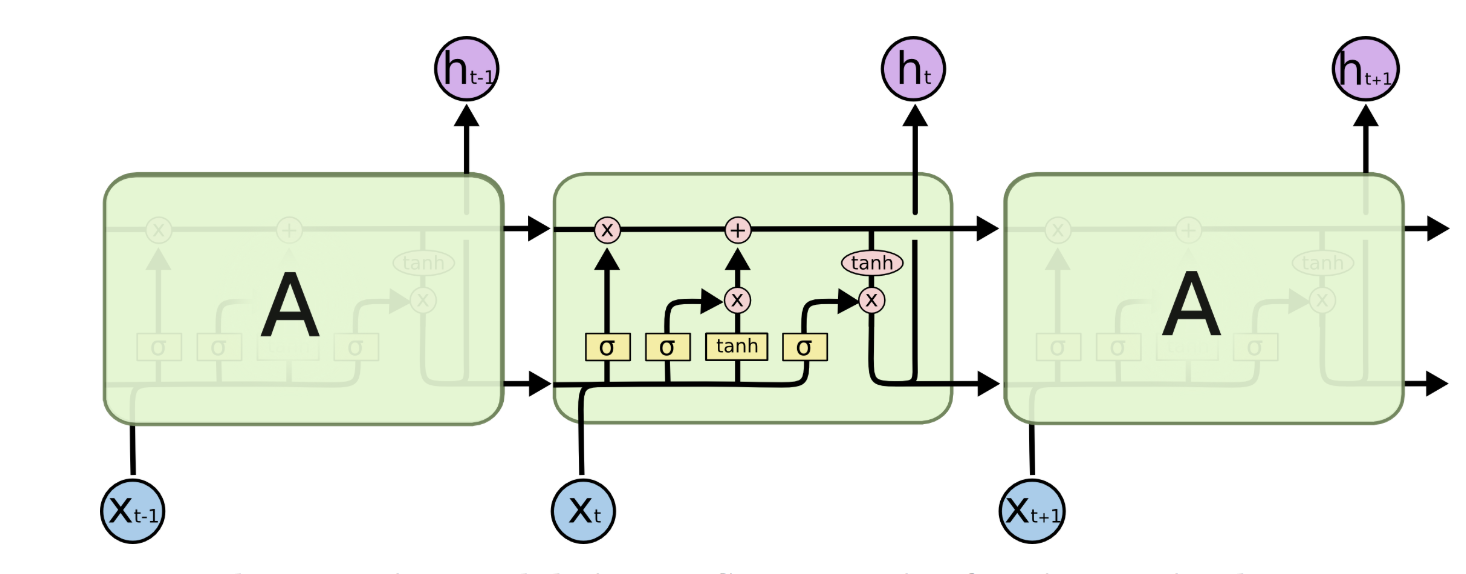
\includegraphics[width=0.8\textwidth,height=4.5cm]{figs/image/lstm.png}
          \caption{
            The repeating module in an LSTM contains four interacting layers.
            \href{http://colah.github.io/posts/2015-08-Understanding-LSTMs/}{Source}
          }
          \label{fig:lstm}
\end{figure}

Long Short Term Memory networks \cite{article-lstm} are a special kind of RNN, capable of learning long-term dependencies. 
They work tremendously well on a large variety of problems, and are now widely used.
LSTMs are explicitly designed to avoid the long-term dependency problem. 
Below is how LSTM works

The forget gate in LSTM is to decide what information we’re going to throw away from the cell state.
\[\vect{f_t} = \sigma(\matr{W_{fh}}\vect{h_{t-1}}+\matr{W_{fx}}\vect{x_t} + \vect{b_f}) \]

Input gate decides which values we’ll update
\[\vect{i_t} = \sigma(\matr{W_{ih}}\vect{h_{t-1}} + \matr{W_{ix}}\vect{x_t} + \vect{b_i})\]

New candidate cell state is to decide what new information we’re going to store in the cell state.
\[\vect{\widetilde{c}_t} = tanh(\matr{W_{ch}}\vect{h_{t-1}} + \matr{W_{cx}}\vect{x_t} + \vect{b_c})\]

New cell state:
\[\vect{c_t} = \vect{f_t}*\vect{c_{t-1}} + \vect{i_t}*\vect{\widetilde{c}_t}\]

Output Gate decides what parts of the cell state we’re going to output.
\[\vect{o_t} = \sigma(\matr{W_{oh}}\vect{h_{t-1}} + \matr{W_{ox}}\vect{x_t} + \vect{b_o})\]

Output:
\[\vect{h_t} = \vect{o_t}*tanh\vect{(c_t)}\]

\section{Gated Recurrent Units}
% Authors: Qintai Liu
% Lecture date: 3/11/2019

\begin{figure}[h]
  \centering
      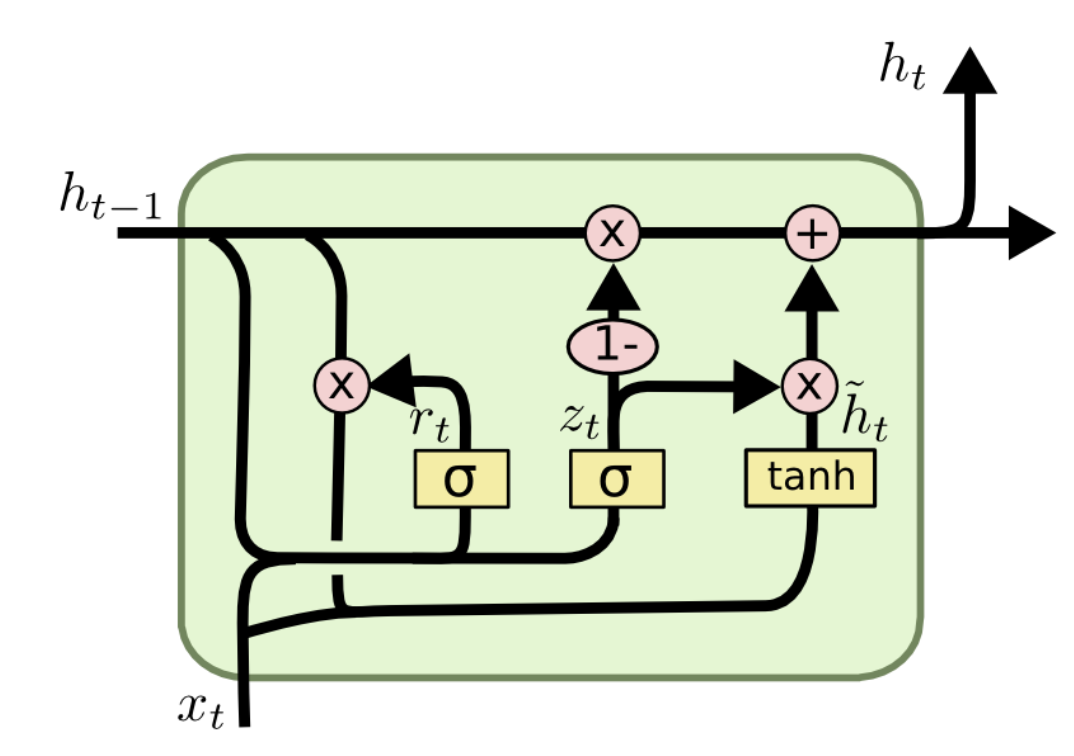
\includegraphics[width=0.5\textwidth,height=4.5cm]{figs/image/GRU.png}
          \caption{
            Gated Recurrent Units
            \href{http://colah.github.io/posts/2015-08-Understanding-LSTMs/}{Source}
          }
          \label{fig:gru}
\end{figure}

A slightly more dramatic variation on the LSTM is the Gated Recurrent Unit \cite{1406.1078}.
It combines the forget and input gates into a single “update gate.” 
It also merges the cell state and hidden state, and makes some other changes. 
The resulting model is simpler than standard LSTM models.
Below is how GRU works

The update gate decides what information from the past would be passed to the next cell state.

\[\vect{z_t} = \sigma(\matr{W_{zh}}\vect{h_{t-1}}+\matr{W_{zx}}\vect{x_t} + \vect{b_z}) \]

The reset gate determine what information would be discarded from previous cell states.

\[\vect{r_t} = \sigma(\matr{W_{rh}}\vect{h_{t-1}}+\matr{W_{rx}}\vect{x_t} + \vect{b_r}) \]

Then the current memory content update the stories the latest important information by using the reset gate.

\[\vect{\widetilde{h}_t} = \tanh(\matr{W_{hr}}(\vect{r_t}*\vect{h_{t-1}}) + \matr{W_{hx}}\vect{x_t} + \vect{b_h})\]

Finally, the final cell state updates the information gained from the current unit and passed it to the next cell.

\[\vect{h_t} = (1-\vect{z_t})*\vect{h_{t-1}} + \vect{z_t}*\vect{\widetilde{h}_t}\]

\chapter{Recurrent Neural Networks}
% Authors: Benjamin Ahlbrand (editor), Xingyu Ding, Haoran Anthony Su, 3/12/19.

\section{ High-Level Overview of Recurrent Neural Networks }

As Convolutional Neural Networks naturally lend themselves to images, RNNs (including LSTMs and Transformers) lend themselves similarly to sequential data (which could additionally include each step being images). These might take the form of time series, speech recognition, learning grammars (language translators, name generators, etcetera) or musical rhythms - among others. More precisely one can define them to be directed graphs mapping to a temporal sequence.\\

Visual captioning \cite{DBLP:journals/corr/VinyalsTBE16} is another interesting application, where they combine RNNs and CNNs in order to attempt to generate a text description of a scene \ref{fig:visual_caption}

\begin{figure}
    \centering
    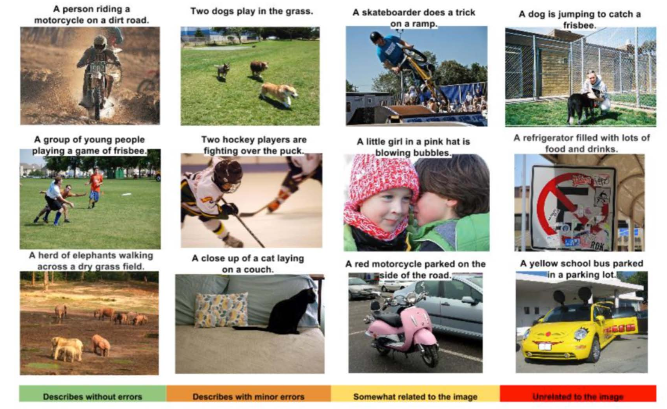
\includegraphics[width=\textwidth]{figs/image_captioning.png}
    \caption{Vinyals et al. (2016) Show \& Tell: Lessons Learned from the 2015 MSCOCO Image Captioning Challenge}
    \label{fig:visual_caption}
\end{figure}

\subsection{Sequence to vector}
Explanation: input: a sequence of words; output: a scalar value or a vector (see Figure \ref{fig:seq_to_vec}).\\
\begin{figure}[ht]
    \centering
    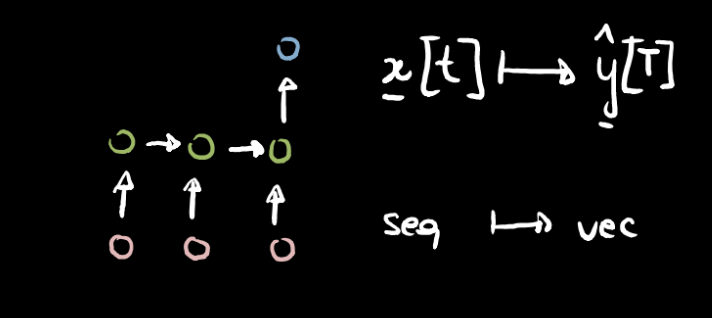
\includegraphics[width=200pt]{figs/seq_to_vec.png}
    \caption{A hand-drawn diagram showing the sequence to vector rationale in the neural networks. Red, green, blue circles are input,hidden,output nodes, respectively. A sequence of inputs are given to the network and there is only one output in the end.}
    \label{fig:seq_to_vec}
\end{figure}
\\
Example: learning to execute (Zaremba \& Sutskever, 2015)\\
Neural network is trained to interpret several lines of python codes and report the result of the running code (see Figure \ref{fig:learning_to_execute}). \\
\begin{figure}[ht]
    \centering
    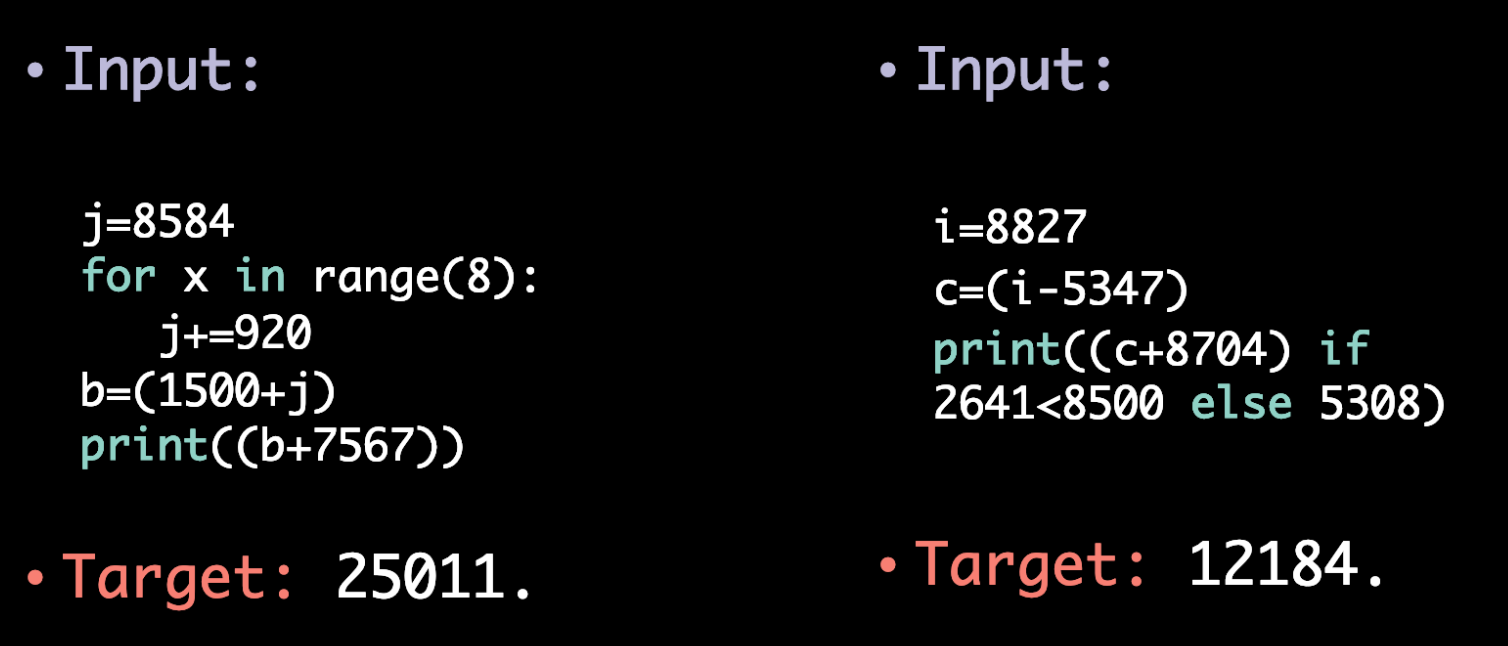
\includegraphics[width=200pt]{figs/learning_to_execute.png}
    \caption{An example of sequence to vector rationale. A paragraph of Python code is given to the network as an input and the execution output of the Python code is supposed to be the output of the network.}
    \label{fig:learning_to_execute}
\end{figure}

\subsection{Sequence to vector to sequence}
Explanation: a sequence of words $\rightarrow$ hidden representations(vector) $\rightarrow$ output sequence (see Figure \ref{fig:seq_to_vec_to_seq}).\\
\begin{figure}[ht]
    \centering
    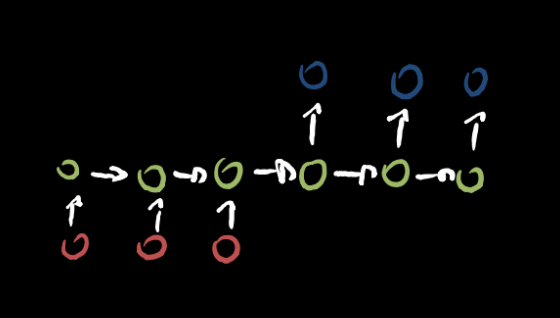
\includegraphics[width=200pt]{figs/seq_to_vec_to_seq.png}
    \caption{A hand-drawn diagram showing the sequence to vector to sequence rationale in the neural networks. Red, green, blue circles are input,hidden,output nodes, respectively. A sequence of inputs are given to the network and used to compute hidden state. Hidden state variable are  then used to generate a sequence of outputs. }
    \label{fig:seq_to_vec_to_seq}
\end{figure}
\\
Example: phrase representation clustering (Cho et al., 2014)\\
Semantically close phrases are close to each other on the representation map (Figure \ref{fig:phrase_representaion})\\
\begin{figure}[ht]
    \centering
    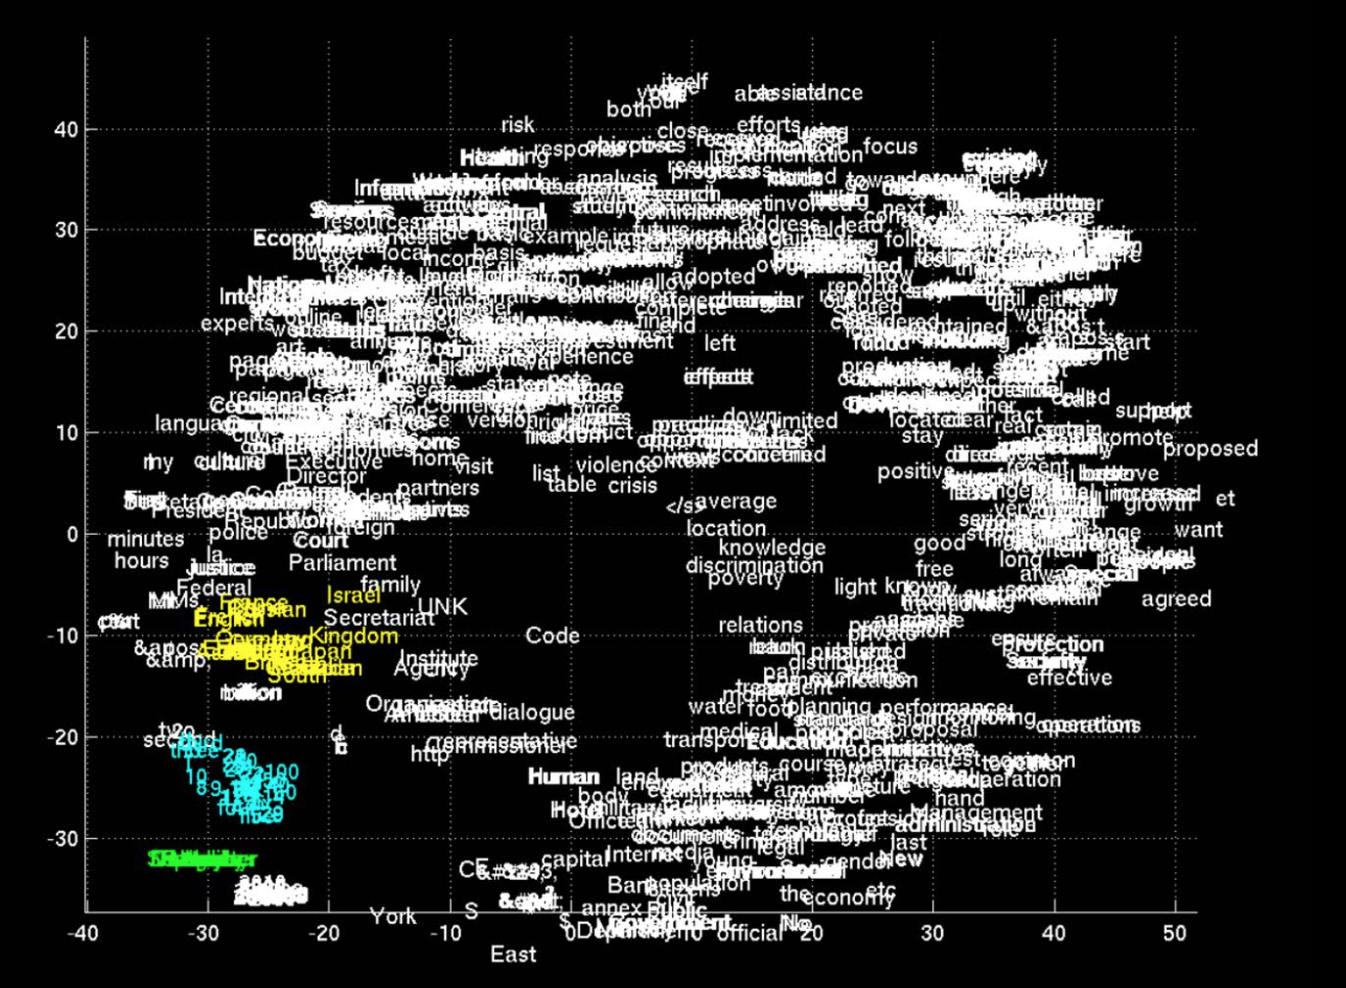
\includegraphics[width=200pt]{figs/phrase_representation.png}
    \caption{An example of sequence to vector to sequence rationale. Words are clustered according to their semantics}
    \label{fig:phrase_representaion}
\end{figure}
One interesting characteristic is one could perform arithmetic calculation of the semantics in hidden variable space. For example, we have\\
\begin{equation*}
    h('king')-h('men')+h('women')=h('queen')
\end{equation*}
where h(X) is the hidden state of word 'X'. \\

\subsection{Sequence to sequence}
Explanation: a sequence of words $\rightarrow$ another sequence of words (see Figure \ref{fig:seq_to_seq}).\\
\begin{figure}[ht]
    \centering
    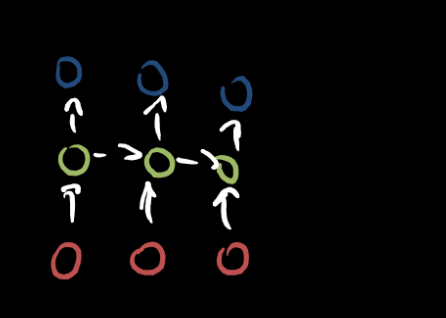
\includegraphics[width=200pt]{figs/seq_to_seq.png}
    \caption{A hand-drawn diagram showing the sequence to sequence rationale in the neural networks. Red, green, blue circles are input, hidden, output nodes, respectively. A sequence of inputs are given to the network and used to compute hidden state. Hidden state variable are used to generate a sequence of outputs in real time.}
    \label{fig:seq_to_seq}
\end{figure}
\\
Example: auto completion: Once a character is typed, there will be a new sequence of suggestions of auto completion. \\
\\
Example: RNN writer(Sloan(2016))\\
Neural network is trained on sci-fi novels and could be used to auto complete the sci-fi novel.\\
Visit \href{github.com/robinsloan/rnn-writer}{github.com/robinsloan/rnn-writer} for more details.\\

\section{RNN training}
\subsection{BPTT: backpropagation through time}
\begin{figure}[ht]
    \centering
    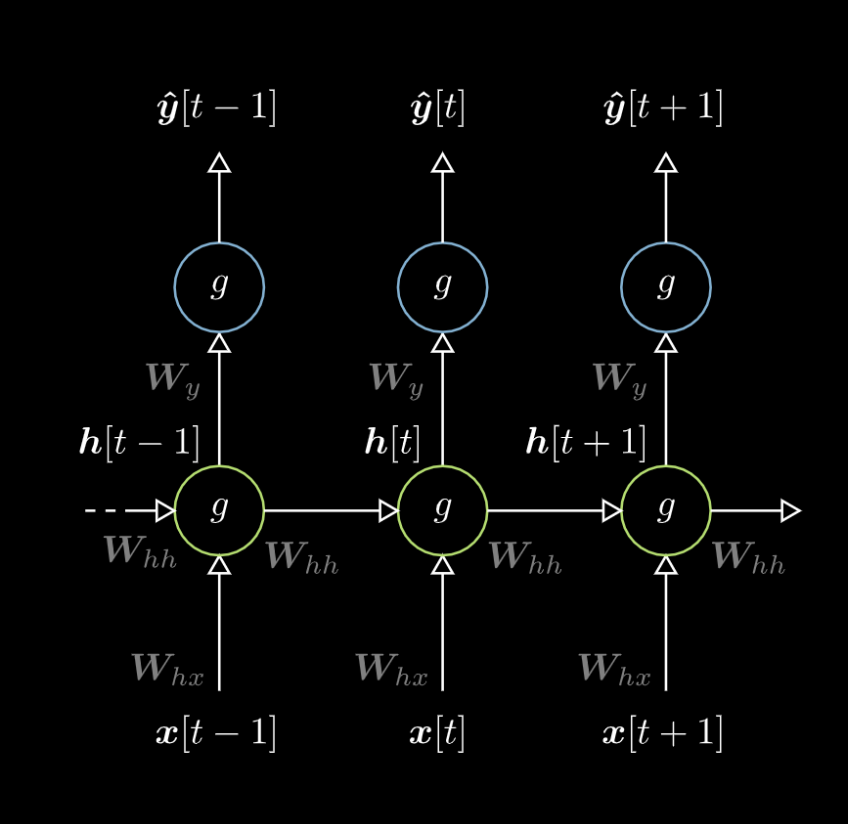
\includegraphics[width=200pt]{figs/bptt.png}
    \caption{A diagram showing how the values are propagated in a RNN. At each time point t, y is calculated using h from the previous time step and current x.  g() is the transfer function, ReLu for example. h[t] is the value of hidden layer at time t. The initial state of h[t] is 0.}
    \label{fig:bptt}
\end{figure}
In order to train a RNN, we are supposed to use backpropagation through time(BPTT) (see Figure \ref{fig:bptt}). In order to calculate the hidden state value h[t], we have\\
\begin{equation}
h[t] = g(W_{hx}x[t]+W_{hh}h[t-1]+b_h)
\end{equation}
To simplify the equation, we define $W_h$ as
\begin{equation}
    W_h = \begin{bmatrix}W_{hx} & W_{hh}\end{bmatrix}
\end{equation}
Thus, we could rewrite equation 1 as 
\begin{equation}
    h[t] = g(W_h\begin{bmatrix}x[t]\\h[t-1]\end{bmatrix} + b_h)
\end{equation}
$\hat{y}[t]$ could be calculated as shown in figure.\ref{fig:bptt_formula} and then we could use normal backpropagation algorithm except that we sum up the gradients at each time step.  
\begin{figure}[ht]
    \centering
    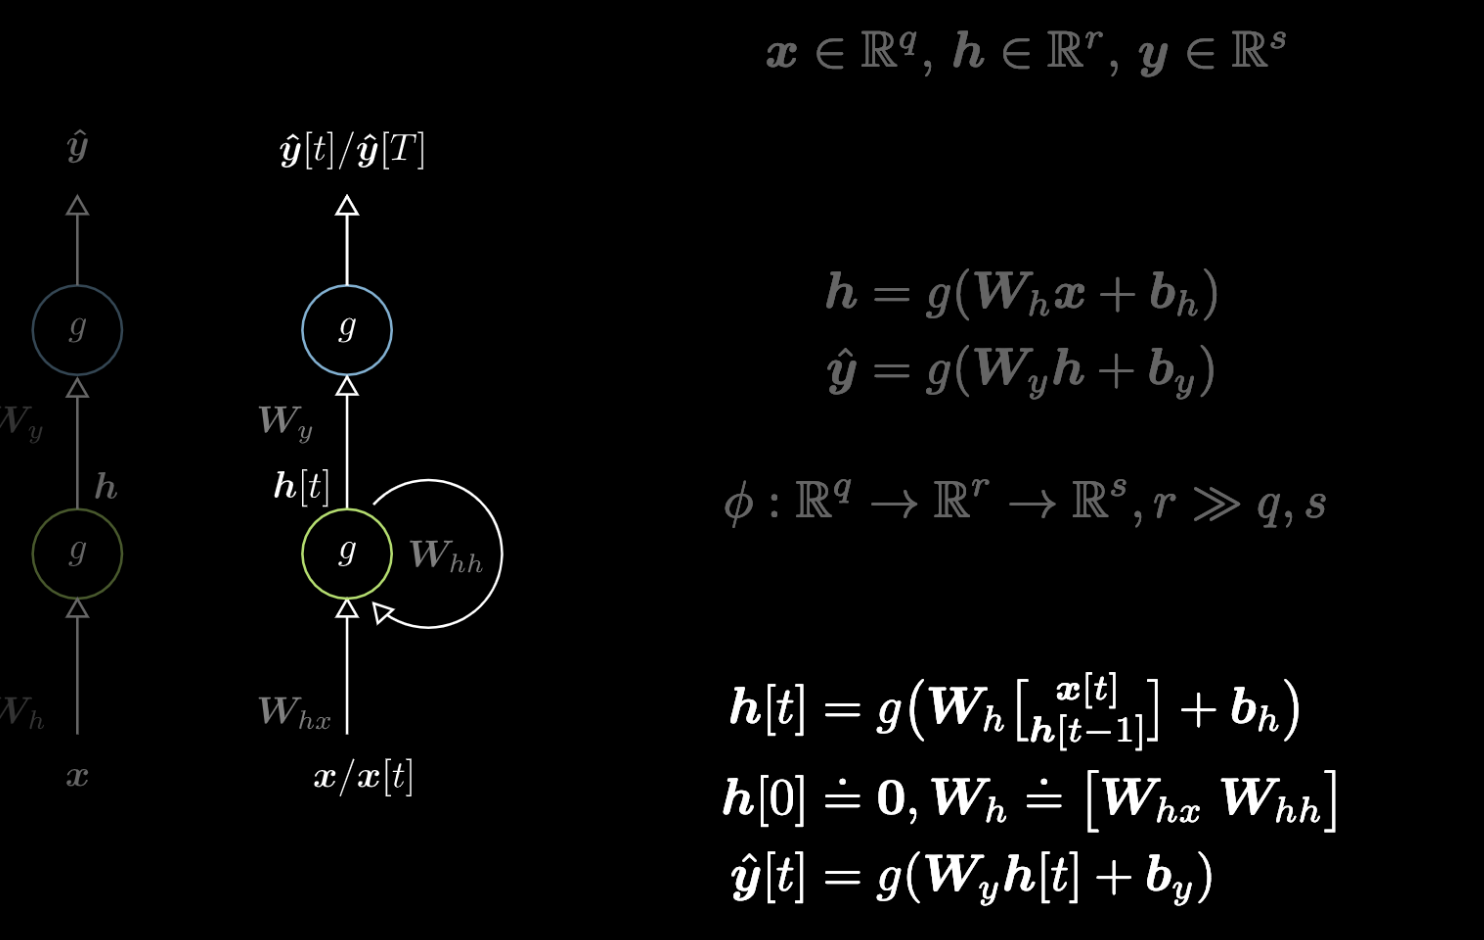
\includegraphics[width=200pt]{figs/bptt_formula.png}
    \caption{$\hat{y}[t]$ shares the same formula as traditional feedforward network. All we have to do is to use the chain rule and backpropagate the error to previous time step.}
    \label{fig:bptt_formula}
\end{figure}


\section{Batch-ification}
When dealing with text sample with large size, we could slice the text into different batches. For example, the batch-ification process for the following sequence of words should exhibit:\\
\begin{align*}
\begin{bmatrix}
    a & g & m & s\\
    b & h & n & t\\
    c & i & o & u\\
    d & j & p & v\\
    e & k & q & w\\
    f & l & r & x\\
\end{bmatrix}
\end{align*}
In this sequence of words, the batch size is 4. We then determine the input and output for our recurrent neural network, namely:\\
\begin{align*}
X[1:T] & = \begin{bmatrix}
        a & g & m & s\\
        b & h & n & t\\
        c & i & o & u\\
\end{bmatrix}
\end{align*}
\begin{align*}
Y[1:T] & = \begin{bmatrix}
        b & h & n & t\\
        c & i & o & u\\
        d & j & p & v\\
\end{bmatrix}
\end{align*}
Notice here $T = 3$ as we proceed three sequence of words. The next step is to perform back-propagation through time on the sequences of words, which is to say we calculate gradient descent horizontally and vertically. Every time we extract one word from the input sequence and we are aiming to predict the corresponding output in the output sequence. For example, when we select $X[1] = [a, g, m, s]$ as input, we train through the RNN to predict $Y[1] = [b, h, n, t]$. At the same time, we send the hidden representation h[1] forward to perform the RNN given $X[2]$ predicting $Y[2]$. After sending the final hidden representation $h[T-1]$ for the final set of $X[T]$ and $Y[T]$, we cut the gradient and conclude the temporal bulk of this batch. \\

The reason behind concluding the temporal bulk after we sending the last hidden representation of the RNN is that we need to stop the gradient descent eventually. Thus, the gradient descent from the following sequences of words is zero.(The PyTorch Auto-grad will handle this critical point.) Similarly, we also don't have the gradient coming from the past sequences before this batch.

\section{Vanishing of the Gradient and GRU}
The limitation of a recurrent Neural Network is the diminishing of the gradient back in time. A very strong gradient would be weakening back through time because of the way we initialize the weight-by selecting very small eigenvalues across zero. A powerful technique that preventing the gradient from vanishing back through time is by employing Gated Recurrent Unit (GRU).\\

GRU uses two gates-update gates and reset gates. A update gate helps the model to determine how information/gradient from the previous time steps need to pass along to the future. A reset gate, on the other hand, determine how much past information/gradient to forget. 

\section{Long Short Term Memory}
Long Short Term Memory, or typically referred to as LSTMs - these are second order RNNs, tend to imbue a sense of locality (spatial, temporal) to the network models.\\

The forward propagation of the RNN are represented by:\\
\begin{align*}
    h[t] & = g(W_{h} \begin{bmatrix}
        x[t] \\
        h[t - 1] \\
    \end{bmatrix}) + b_{h}\\
    \bar{y}[t] & = g(W_{y}h[t] + b_{y})
\end{align*}
The decomposition of a Gated Recurrent Unit (GRU) will be visualized as:\\
\begin{align*}
i[t] & = \sigma(W_{i} \begin{bmatrix} x[t] \\ h[t - 1] \\ \end{bmatrix}) + b_{i}\\
f[t] & = \sigma(W_{f} \begin{bmatrix} x[t] \\ h[t - 1] \\ \end{bmatrix}) + b_{f}\\ 
o[t] & = \sigma(W_{o} \begin{bmatrix} x[t] \\ h[t - 1] \\ \end{bmatrix}) + b_{o}\\
\bar{c}[t] & = \tanh(W_{c} \begin{bmatrix} x[t] \\ h[t - 1] \\ \end{bmatrix}) + b_{c}\\
c[t] & = f[t] \odot c[t-1] + i[t] \odot \bar{c}[t]\\
h[t] & = o[t] \odot \tanh(c[t])\\
\end{align*}
To control the output, take saturated (squashing / squeezing inputs to a range) sigmoid as an example which we could make the switch simply as 1 or 0, we could determine the hidden representation to be zero by setting the sigmoid function to be null; On the other hand, we could output accordingly by setting the sigmoid function to be 1.\\

To control the memory, we could manipulate the input network and the "don't forget" gate. Simply setting them both to zero, we could reset the memory. To keep the memory, we set the input unit to be zero and memory to be one using the sigmoid function to keep the memory without adding anything from the current input. Finally, we could write to the memory by setting the saturated sigmoid function both to be one to add input to the memory.\\

\section{ Transformers? Pay Attention! }
A new architecture has found popularity in many applications typically dominated by RNNs and LSTMs, Transformers - introduced by \cite{DBLP:journals/corr/VaswaniSPUJGKP17}. Transformers essentially add attention 
RNNs and LSTMs suffer issues with the memory bandwidth bound computations in training, where given the orthogonality of traditional convolutional networks to the GPU hardware, CNNs map perfectly to GPUs. Contrarily these hierachical (sometimes) sequential representations don't typically map quite so easily, and hence, performance suffers as a result.\\

\chapter{Long term vs short term memory}

\section{Why Is RNN Useful, And What Are The Drawbacks?}
%Authors: Sarthak Agarwal, Raghav Jajodia, Ieshan Vaidya
%2019-03-31

In lab8 we saw that RNN is useful to learn dependencies over time, and hence can model time dependent sequences effectively.
This means RNN can store context/history at any given time t, which can be used along with the input to predict the output. 
More details about RNN can be found in \hyperref[sec:SimpleRecNet]{Section 13.1}.


However, practically we observe that as the sequence length grows over time, RNN is not able to learn long term dependencies.
This is because of the \textbf{vanishing/exploding gradient} during \textbf{back-propagation through time}.
Back-propagation through time is the method of calculating gradients by unfolding the network in time and then applying normal back-propagation to the unfolded network.
If the the length of input sequence is large, then network is unfolded many number of times.
The consequence of this is that during back-propagation, gradient is multiplied many times (more the sequence length, more the number of multiplications). 


This causes the, gradient to either explode or vanish, which is undesirable.
To solve the issue of exploding gradient, we generally "clip" the gradient to avoid growing it bigger than a threshold value.
However RNN performs poorly for large length sequences because of vanishing gradient problem.

\section{Why Is LSTM Useful?}
%Authors: Sarthak Agarwal, Raghav Jajodia, Ieshan Vaidya
%2019-03-31
Vanishing gradient problem can be solved efficiently by using LSTMs.
LSTM stands for Long Short term Memory and it has been proven effective to model long term dependencies more effectively than RNN, meaning that LSTM has greater memory than RNN.
The reason for this is that LSTMs maintain a cell state which runs straight down the entire chain, with only some minor linear interactions.
They have the ability to either add or remove information to this cell state using gates namely the forget, input  and output gates.
More details about LSTM can be found \hyperref[sec:long-short-term-memory]{here}


The reason why vanishing gradient is handled better in case of LSTM is that gradient flows back effectively through the network because of the presence of relevant gates which makes it very easy for information to just flow along the cell state unchanged.


\section{Lab 8 - Result Analysis}
%Authors: Sarthak Agarwal, Raghav Jajodia, Ieshan Vaidya
%2019-03-31
In lab8, we try to classify a sequence of characters into categories Q,R,S,U. 
This classification is done on the basis of two characters X,Y which can be present anywhere in the sequence. 
In this experiment we compare the ability of RNN and LSTM to learn dependencies for different sequence lengths. The Difficulty and configurations of the experiment is explained in detail in \cref{sec:SeqClassification}. Here is the table of the test accuracies - 

\begin{center}
\begin{tabular}{ | p{3cm} | p{2cm} | p{2cm} | p{2cm} | p{2cm} | }
 \hline
   \textbf{DIFFICULTY} & \textbf{RNN (10 epochs)} & \textbf{LSTM (10 epochs)} & \textbf{RNN (100 epochs)} & \textbf{LSTM (100 epochs)} \\ 
 \hline
 \textbf{Easy} & 60.58\% & 79.33\% & 87.30\% & 87.50\% \\
 \hline
\textbf{Normal} & 24\% & 26\% & 71\% & 85\% \\ 
 \hline
 \textbf{Moderate} & 24.60\% & 28.43\% & 26.65\% & 84.37\% \\ 
 \hline
 \textbf{Hard} & 23.19\% & 25.10\% & 24.70\% & 25.30\% \\ 
 \hline
\end{tabular}

\end{center}
As we can see that LSTM outperforms RNN in almost all the cases.
We also observe that RNN and LSTM are not able to learn the sequence when ran for 10 epochs in case of MODERATE, NORMAL and HARD LEVEL.
When ran for 100 epochs, RNN and LSTM are not able to learn for HARD level, whereas they are able to learn other configurations. 
\chapter{Graph CNN and spectral networks}
% \author{Yuqiong Li}
% \date{March 2019}

\section{Why do CNNs work so well}
% Authors: Yuqiong Li
% Lecture date: 3/11/2019
CNNs have worked well on Euclidean structures (e.g. a regular grid) because of the following properties:
\begin{enumerate}
    \item Images, videos and speeches have translation invariant properties. For example, one can consider images as sampled instances from distributions on the Euclidean space. They are stationary in that they are shift-invariant. 
    \item Images are scale separation 
    \item Features are usually localized, meaning they are much smaller than the input image
    \item CNNs have a fixed number of parameters 
    \item With advancement in graphic gards, CNNs can be computed efficiently 
\end{enumerate}
However, it is not immediately obvious how to extend CNNs to graphs because they do not have these properties as in Euclidean space.

\section{Extend CNN on Graphs}
% Authors: Yuqiong Li
% Lecture date: 3/11/2019
\subsection{A bit of graph theories}

\begin{enumerate}
    \item A weighted undirected graph G with
vertices $V = {1, . . . , n}$, edges $E \subseteq V × V$
and edge weights $wij \geq 0$ for $(i, j) \in E$. 
    \item We can define functions over the vertices $L^2(V) = {V \to R}$, which is also a vectors $f = (f_1, . . . , f_n)$.
    \item We can define the unnormalized Laplacian for $f$ as $(\bigtriangleup f)_i = \sum_{j: (i, j)\in E} w_{ij} (f_i - f_j) $ which is the difference of $f$ and its local average. 
\end{enumerate}

By doing eigendecomposition of a graph Laplacian, we can obtain the its orthogonal eigenvectors as well as the corresponding non-negative eigenvalues.

\subsection{Fourier analysis on Euclidean spaces}
A function $f : [−π, π] → R$ can be written as a Fourier series as the following formula:
\begin{align} 
    f(x) = \sum_{k \geq 0} \langle f, e^{ikx} \rangle_{L^2([-\pi, \pi]) e^{ikx}}
\end{align}
and the corresponding Fourier basis are the Laplacian eigenfunctions: $k^2 e^{ikx}$


\subsection{Fourier analysis on graphs }
A function $f : V \to R$ can be written as a Fourier series as the following formula:
\begin{align} 
    f(x) = \sum_{k=1}^{n} \langle f, \phi_k \rangle_{L^2(V) \phi_k}
\end{align}
and the corresponding Fourier basis are the Laplacian eigenfunctions: $\lambda_k \phi_k$ with $\lambda_k$ being the frequency.

\subsection{Convolution on Euclidean space }
Given two functions $f, g \in [-\pi, \pi] \to R$, their convolution can be written as 
\begin{align} 
    (f \star g) (x) = \int_{-\pi}^{\pi} f(x') g(x-x') dx'
\end{align}

\subsection{Spectral convolution}
Finally, spectral convolution can be defined by analogy to convolution on Euclidean space as 
\begin{align} 
    (f \star g) (x) = \sum{k\geq 1} \langle f, \phi_k \rangle_{L^2_(v)}\phi_k
\end{align}
which is the inverse Fourier transform. 
\chapter{Bayesian Neural Networks}
% Authors: Jong Yeob Kim (editor), Zilin Bian, Di Sha, 4/23/19.

\section{ Motivation of estimating a predictive distribution }

Most of modern neural network models produce point estimation, even though at last phase of image classification models we get confidence scores of different categories like cat and dogs. With complexity/uncertainties happening all the time around the world, it is not always reasonable to get a single output result. Sometimes we cannot tell whether the new model is making sensible predictions or just guessing at random. In this situation, we may wish to get a predictive distribution of results instead of a point estimation.\\

\section{Motivation of caring about uncertainty}

Given several pictures of cats and dogs, then being asked to classify a new cat photo, we should return a prediction with rather high confidence. But if we are given a photo of an ostrich and force our hand to decide if it is a cat or dog, we should return a prediction with very low confidence. It is quite important to say whether we are confident about our estimation or not. Another example is predicting physics simulator. In physics, you may have simulators for predicting the trajectory of some particles or accelerators. But, then this simulation takes forever. In this case, you can use neural networks to speed up computations and getting approximate values. The network is trained over many iterations using data provided by simulators. However, if inputs are far from trained data, a prediction is made with higher uncertainty. Furthermore, this sort of information lies at the foundations of artificial intelligence as well. For example, a Roomba vacuum needs to learn about its environment (e.g. living room) based on its actions (rolling around in different directions). It can decide to go forward and might bump into a wall. One should enable reward mechanism to encourage it when it learns to avoid the wall or penalize it when it crahses into a sofa. This setting is known as reinforcement learning. The Roomba is requried to explore its environment looking for these rewards, and that's where uncertainty comes into play. The Roomba will try to minimise its uncertainty about different actions - and trade-off between this exploration, and exploitation of what it already knows. You can trace to \href{https://cs.stanford.edu/people/karpathy/convnetjs/demo/rldemo.html}{Karpathy's} interactive demo to learn into this Roomba play.

\section{Get predictive distribution using dropout}

Take any network trained with dropout and some input $x^*$. We are looking for the expected model output given our input - the predictive mean $\mathbb{E}(y^*)$ and how much the model is confident in its prediction - the predictive variance $Var(y^*)$. The neural network model with enabled dropout in both train and test phases will be equivalent to Gaussian process approximation. In the following section we will walk through the process of enabling dropout and getting the estimation of predictive distribution.\\
First, define a prior length-scale $l$. This captures our belief over the function frequency. A short length-scale $l$ corresponds to high frequency data, and a long length-scale corresponds to low frequency data.Take the length-scale squared, and divide it by the weight decay. We then scale the result by half the dropout probability over the number of data points. Mathematically this result in a Gaussian process precision $\tau = \frac{l^2 p}{2N \lambda}$ we mentioned above. Note that $p$ here is the probability of the units not being dropped - in most implementations $p_{code}$ is defined as the probability of the units to be dropped, thus $p := 1- p_{code}$ should be used when calculating $\tau$. Next, simulate a network output with input $x^*$, treating dropout as if we were using it during training phase. This means enabling dropout also in test phase. Repeat this $T$ times with different units dropped every time, and collect the results ${\hat{y_t}^* (x^*)}$. These are empirical samples from our approximate predictive posterior. We can get an empirical estimator for the predictive mean of our approximate posterior as well as the predictive variance (our uncertainty) from these samples. Mathematically, averaging forward passes through the network is equivalent to Monte Carlo integration over a Gaussian process posterior approximation. The derivation is provided in \cite{gal2016dropout}. The process of applying dropout into the neural network at both training and test phases is thus called Monte-Carlo dropout (MC dropout). We simply follow these two equations:
\begin{equation}
    \mathbb{E} (y^*) \approx \frac{1}{T} \sum^{T}_{t=1} \hat{y_t}^*(x^*)
\end{equation}
\begin{equation}
    Var(y^*) \approx \tau^{-1} I_D + \frac{1}{T}\sum^{T}_{t=1} \hat{y_t}^*(x^*)^T \hat{y_t}^* (x^*) - \mathbb{E} (y^*)^T \mathbb{E} (y^*)
\end{equation}
\\
Eq. 17.1 was introduced as model averaging and it was explained that scaling the weights at test time without dropout gives a reasonable approximation to this equation. Eq. 17.2 is simply the sample variance of $T$ forward passes through the network plus the inverse model precision. Note that the vectors above are row vectors and that the products are outer-products.
\\
Implementation in python code to get the predictive mean and uncertainty is easy:

\begin{minted}{python}
Probs = []
for _ in range(T):
    probs += [model.output_probs(input_x)]
predictive_mean = numpy.mean(prob, axis=0)
predictive_variance = numpy.var(prob, axis=0)
tau = 1**2*(1 - model.p)/ (2*N*model.weight_decay)
predictive_variance += tau**-1
\end{minted}

\section{Understanding MC dropout Models}
\subsection{Regression}
To see what the uncertainty looks like where points are far away from training data, we can visualize it using a simple one dimensional regression model with a subset of the atmospheric CO$_2$ concentrations dataset. This dataset was derived from situ air samples collected at Mauna Loa Observatory, Hawaii, since 1958. The dataset consists of about 200 data points and has been centered and normalized. Fig. \ref{fig:co2_concentration} shows the raw data, and \ref{fig:regression_without_uncertainty} shows the processed training data (in red, left of the dashed blue line) and a missing section to the right of the dashed blue line. A neural network with 5 hidden layers, 1024 units in each layer, and ReLU non-linearities, and dropout with probability 0.1 after each weight layer, was fitted to the data.

\begin{figure}[H]
    \centering
    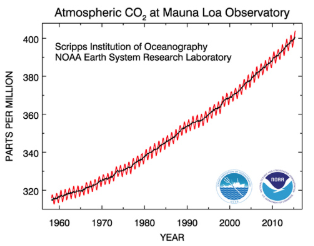
\includegraphics[width=10cm]{figs/CO2 concentration.png}
    \caption{CO$_2$ dataset before pre-processing}
    \label{fig:co2_concentration}
\end{figure}

\begin{figure}[H]
    \centering
    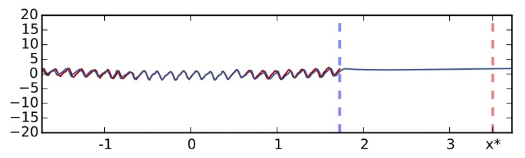
\includegraphics[width=10cm]{figs/Regression without uncertainty.png}
    \caption{Standard dropout network without using uncertainty information}
    \label{fig:regression_without_uncertainty}
\end{figure}

The point marked with a dashed red line is a point far away from the training data. As can be seen, standard dropout confidently predicts a clearly insensible value for the point, as the function is obviously periodic. Therefore, it is really hard to tell whether the model can be trusted or not. However, if we add the uncertainty information introduced above to the exactly same network (we don't need to re-train the model, just perform predictions in a different way), we can get the revealing information shown in Fig. \ref{fig:regression_with_uncertainty}.

\begin{figure}[H]
    \centering
    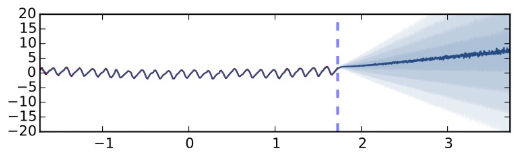
\includegraphics[width=10cm]{figs/Regression with uncertainty.png}
    \caption{Same dropout network performing predictions using uncertainty information}
    \label{fig:regression_with_uncertainty}
\end{figure}

As can be seen, the model does capture a large amount of uncertainty information about the far away test point. This uncertainty information is very similar with that of a Gaussian process model with a squared exponential covariance function (as shown in Fig. \ref{fig:regression_GP}). Though the estimate is different, the uncertainty still increases as the test point goes farther from the training data. It's not surprising that the uncertainty looks different, since the ReLU non-linearity corresponds to a different Gaussian process covariance function. If we change the non-linearity to a TanH non-linearity, the result looks as shown in Fig. \ref{fig:regression_tanh}.

\begin{figure}[H]
    \centering
    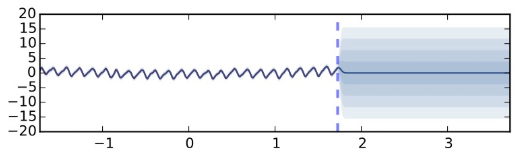
\includegraphics[width=10cm]{figs/Regression using Gaussian Process.png}
    \caption{Gaussian process with SE covariance function on the same dataset}
    \label{fig:regression_GP}
\end{figure}

\begin{figure}[H]
    \centering
    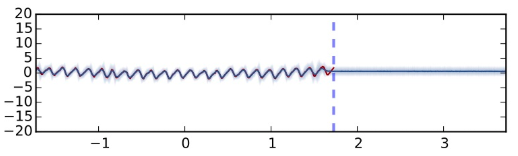
\includegraphics[width=10cm]{figs/Regression using TanH.png}
    \caption{Dropout network using uncertainty information and TanH non-linearity}
    \label{fig:regression_tanh}
\end{figure}

This time it seems that the uncertainty doesn't increase as farther from the training data. This might be because TanH saturates whereas ReLU does not. This non-linearity will not be appropriate for tasks where we are expecting the uncertainty to increase as the test point goes farther away from the training data.

\subsection{Classification}
This section takes an example of image classification using MNIST digits dataset and the popular LeNet convolutional neural network. In this model the prediction is fed into a softmax which gives probabilities for different classes (the 10 digits). However, these probabilities are not enough to see if the model is certain in its prediction or not. This is because the standard model would pass the predictive mean through the softmax rather than the entire distribution.

If we take an idealized binary classification example (as shown in Fig. \ref{fig:classification_binary}). Passing a point estimate of the mean of a function (a TanH function for simplicity, solid line on the left) through a softmax (solid line on the right) results in highly confident extrapolations with $x^*$ (a point far from the training data) classified as Class 1 with probability 1. However, passing the distribution (shaded area on the left) through a softmax (shaded area on the right) reflects classification uncertainty better at points far from the training data. Taking the mean of this distribution passed through the softmax we get Class 1 with probability 0.5 -- the model's true prediction.

\begin{figure}[H]
    \centering
    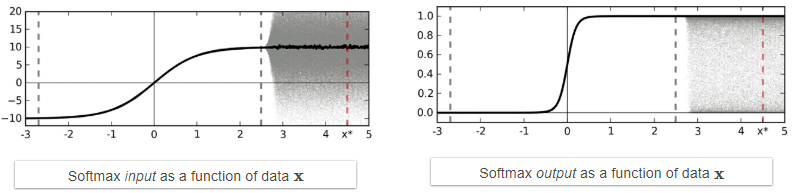
\includegraphics[width=\textwidth]{figs/Classification_binary.png}
    \caption{A sketch of softmax input and output for an idealized binary classification problem}
    \label{fig:classification_binary}
\end{figure}

Then we can try passing the entire distribution through the softmax instead of the mean alone. The samples are simulated through the network and the softmax output is averaged. The convolutional neural network is trained over MNIST with dropout applied after the last inner-product layer (with probability 0.5). The model predictions are evaluated over the following sequence of images (Fig. \ref{fig:classification_input}), that correspond to some projection in the image space.

\begin{figure}[H]
    \centering
    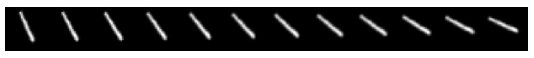
\includegraphics[width=10cm]{figs/Classification_input.png}
    \caption{Image inputs (a rotated digit) to the dropout LeNet network}
    \label{fig:classification_input}
\end{figure}

These images correspond to the $X$ axis in the idealized depiction above. A histogram of 100 samples obtained by simulating forward passes through the dropout LeNet network is shown in Fig. \ref{fig:classification_multi}. As can be seen, Class 7 has low uncertainty for the right-most images. This is because the uncertainty ``envelope" of the softmax input for these images is far away from the envelopes of all other classes. In contrast, the uncertainty envelope of Class 5 for the middle images interests the envelopes of some of the other classes (even though its mean is higher) -- resulting in large uncertainty for the softmax output. It is important to note that the model uncertainty in the softmax output can be summarized by taking the mean of the distribution. In the idealized example above, this would result in softmax output 0.5 for point $x^*$ (instead of softmax output 1) and here it will result in a lower softmax output that might result in a different image class. This sort of information can help us in classification tasks: obtaining higher classification accuracies. It also helps us analyze our model and decide whether we have enough data or if the model is specified correctly.

\begin{figure}[H]
    \centering
    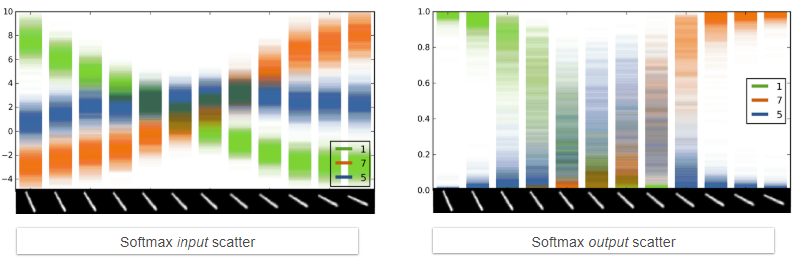
\includegraphics[width=\textwidth]{figs/Classification_multi.png}
    \caption{A sketch of 100 forward passes of the softmax input and output for dropout LeNet}
    \label{fig:classification_multi}
\end{figure}


%%%%%%%%%%%%%%%%%%%%%%%%%%%%%%%%%%%%%%%%%%
\part{Practical \& applications}\label{prt:prct}
%%%%%%%%%%%%%%%%%%%%%%%%%%%%%%%%%%%%%%%%%%
\chapter{Backprop In Practice}\label{chp:Backprop in Practice}
% Authors: tn1050@nyu.edu, vy404@nyu.edu, sk7685@nyu.edu.
% Lecture date: 2.4.19
\setlength{\abovedisplayskip}{7pt}
\setlength{\belowdisplayskip}{7pt}

% Authors: tn1050@nyu.edu, vy404@nyu.edu, sk7685@nyu.edu.
% Lecture date: 2.4.19
\section{Use of ReLU non-linearities}
Non-linear transformations are an essential part of the deep neural networks as discussed in the Chapter 3. An artificial neuron does not know the bounds of its values and can not decide whether it should fire or not, we use activation functions to check the value 
\begin{equation}
    Y = \sum (W * X_{in}) + C
\end{equation}

produced by the neuron and decide if the neuron is fired or not. 
\begin{enumerate}[label=(\alph*)]
\item The step function is a threshold based activation function Activation function. 
\begin{equation}
    f(x)=\begin{cases}
            \text{activated}, & Y > \text{threshold} \\
            \text{deactivated}, & Y < \text{threshold}
        \end{cases}
\end{equation}

However the step function does not account for partial activation which can help learning become smoother and easier (less wiggly). It also has zero gradients, which makes it hard to train in practical setting. As an alternative, people used sigmoid or hyperbolic tangent non-linearities in neural networks, which are saturating functions. 
\begin{figure}[ht]
\centering
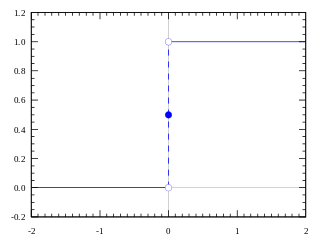
\includegraphics[width=50mm]{figs/step_function.png}
\caption{Unit Step Function}
\label{fig:step_function}
\end{figure}

\item The sigmoid function is a mathematical function having an "S" shaped curve (sigmoid curve).
\begin{equation}
    f(x) = \frac{1}{1+e^{-x}}
\end{equation}
has a problem of vanishing gradients towards either end of the function causing the network to stop learning or to learn at a very slow rate.

\begin{figure}[ht]
\centering
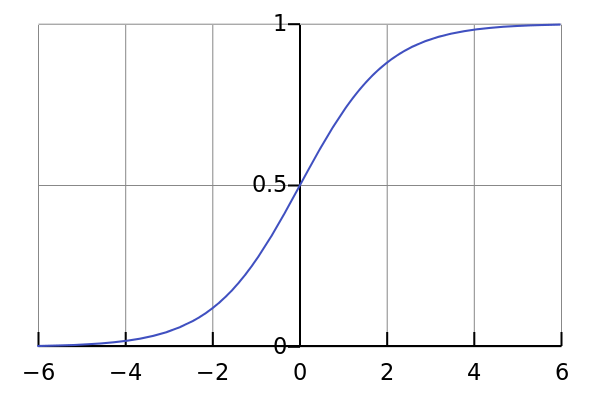
\includegraphics[width=50mm]{figs/sigmoid_function.png}
\caption{Sigmoid Function}
\label{fig:sigmoid}
\end{figure}

\item The tanh function also has vanishing gradient characteristics similar to sigmoid function,
\begin{equation}
    f(x) = \frac{2}{(1+e^{-2x})}-1
\end{equation}
but it presents an improvement over the sigmoid by extending to negative values and avoiding bias in the gradients. 
However its gradient characteristics hinders our ability to train deeper neural network and for this reason, they fell out of favor and using ReLU non-linearities enabled us to train much deeper networks. 

\begin{figure}[ht]
\centering
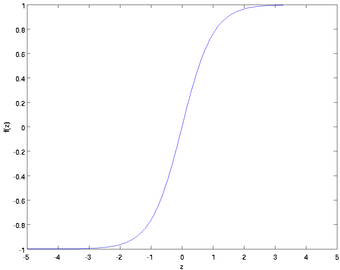
\includegraphics[width=50mm]{figs/tanh_function.png}
\caption{tanh Function}
\label{fig:tanh}
\end{figure}

\item The Rectified Linear Unit is an activation function defined as 
\begin{equation}
    f(x) = \max (0,x)
\end{equation}
where x is the input to a neuron giving an output x if x is positive and 0 otherwise. 
This promotes a reduced likelihood of encountering vanishing gradient problems. When $a > 0$, the gradient has a constant value. 
In contrast, the gradient of sigmoids becomes increasingly small as the absolute value of x increases.
The constant gradient of ReLUs results in faster learning.

ReLU also helps with increasing the sparsity of the network which arises when $a ≤ 0$. 
As the number of such units increase in a layer, it leads to a sparse representation. 
Sigmoids on the other hand are always likely to generate some non-zero value resulting in dense representations. 
The range of values can also be infinite.

ReLU is analogous to half-wave rectification in electrical engineering and has been the most popular activation function to this day.

\begin{figure}[ht]
\centering
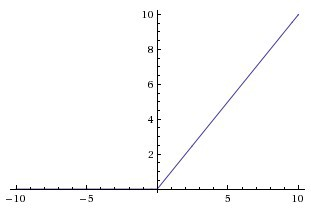
\includegraphics[width=50mm]{figs/ReLU_function.jpg}
\caption{ReLU Function}
\label{fig:relu}
\end{figure}
\end{enumerate}

{\centering\fbox{\begin{minipage}{30em}
\centering\textbf{Use of ReLU non-linearities}
\begin{enumerate}
    \item ReLU nonlinearities learns much faster than the standard sigmoid function and improves our ability to train deeper neural networks.
    \item Also helps with increasing the sparsity of network as the neuron is switched off for $a \leq 0$
\end{enumerate}
\end{minipage}}\par}

% Authors: tn1050@nyu.edu, vy404@nyu.edu, sk7685@nyu.edu. 
% Lecture date: 2.4.19
\section{Use cross-entropy loss for classification}
When we work on classification problems we use cross-entropy loss which measures performance of a classification model whose output is a probability value. 
The cross entropy loss increases as the predicted probability moves away from the actual label. 
Log loss penalizes all errors however gives higher penalty to the predictions that are confident and wrong. 
It is defined as,
\begin{equation}
H(y, p)=-\sum_i y_i \log(p_i)
\end{equation}
we calculate a separate loss for each class label per observation and sum the result. 
Cross entropy measure is a widely used alternative of squared error.

Log softmax is a special case of cross entropy loss where only one value in the output array is $1$ and the others are $0$. 
The more general form calculates the cross-entropy between two discrete distributions which log-softmax doesn’t compute. 
Softmax is often the best option to use for classification problems. 

{\centering\fbox{\begin{minipage}{30em}
\centering\textbf{Use cross-entropy loss for classification}
\begin{enumerate}
    \item Cross entropy loss increases as the predicted probability moves away from the actual label.
    \item Log softmax is a special case of cross entropy loss.
\end{enumerate}
\end{minipage}}\par}
\vspace{5pt}


% Authors: tn1050@nyu.edu, vy404@nyu.edu, sk7685@nyu.edu. 
% Lecture date: 2.4.19 
\section{Use Stochastic Gradient on Minibatches}
The standard gradient descent algorithm updates the model parameters $θ$ in the following way: 
% θ=θ−α∇θE[J(θ)] 
\begin{equation}
    \theta = \theta - \alpha\bigtriangledown\theta E [J(\theta)]
\end{equation}
where the expectation in the above equation is approximated by evaluating the cost and gradient over the full training set. 
Stochastic Gradient Descent (SGD) simply does away with the expectation in the update and computes the gradient of the parameters using only a single or a few training examples. 
An estimate of the true gradient is computed based on the error $E^t$ of that example, and the weights are updated in the following way: 
% W(t+1) = W(t) - ndel E^t/del W. 
\begin{equation}
    W(t+1) = W(t) - \eta \dfrac{\delta E^t}{\delta W}
\end{equation}
Generally each parameter update in SGD is computed w.r.t a few training examples or a minibatch as opposed to a single example. 

\begin{figure}[ht]
\centering
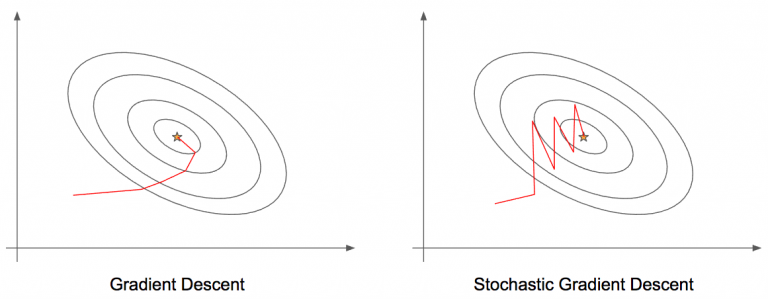
\includegraphics[width=120mm]{figs/Stochastic.png}
\caption{Gradient Descent vs. Stochastic Gradient Descent}
\label{fig:sgd}
\end{figure}
We do forward and backward propagation on a small group of samples, compute their average gradients which are then used to update the model parameters. 
We then take the next group of samples and repeat this process. The two limit cases are when the size of the batch is one or the size of the batch is the entire training set. 
It is inefficient to use the entire training set to compute the gradient as there might be many redundant samples in the training set. 
For instance, if a training set contains one million samples which are just repetition of ten-thousand images hundred times, then by using the full batch gradient-descent we will be using hundred times the number of resources computing the gradient than we should. 

We do not have such training sets in real life. However, we often have a lot of samples that are very redundant. 
For instance, while doing character recognition on MNIST dataset, we will have a lot of ones very very similar to each other (with very minor variations). 
Similarly, ImageNet has many pictures where samples within the same category are very similar to each other. 
On large datasets, SGD can converge faster than batch training because it performs updates more frequently.
We can get away with this because the data often contains redundant information, so the gradient can be reasonably approximated without using the full dataset. 
If there were no redundancy we wouldn’t be able to learn any generalizable information.

However, in the presence of redundancy if we calculate the gradient on the entire training set we will be doing more computation than necessary. 
There has been some research done on the optimal size of a batch. 
There is an argument that small batch sizes put a lot of noise in the gradients, which in turn changes the weights more and produces a  regularization effect that leads to better generalization error.

Another factor in determining the batch size is how well we can saturate the current hardware.
Generally, the calculation in a neural net is not limited by the speed of the processor but is limited by how fast you can shuffle data in and out of the processor to and from the memory. 
Minibatch training can be faster than training on single data points because it can take advantage of vectorized operations to process the entire minibatch at once. 
How we organize the calculation within a GPU allows us to take advantage of their cache. 
One good way to optimize memory bandwidth is to use matrix multiplication at the lowest level (matrix multiplication is an operation that has a large number of operations per memory access thus we organize data in such a way that for every piece of data we load from memory we do a lot of operations with them).

In general, we use the smallest batch size that will saturate the hardware. 
Another factor that comes into consideration is parallelization. 
The simplest way to parallelize the training of a neural net is to take a large batch,  divide it into chunks and give each chunk to a separate GPU. 
Their gradients will then be averaged and used for updating the model parameters, which are then distributed to each of the workers (synchronous distributed SGD).

{\centering\fbox{\begin{minipage}{30em}
\centering\textbf{Stochastic Learning with minibatches}
\begin{enumerate}
    \item Stochastic learning is usually much faster and uses lesser resources than batch learning.
    \item Stochastic learning often results in better solutions than batch learning that produce less generalization error
    \item As a rule of thumb, we can use the samllest batch size that will saturate the hardware.
\end{enumerate}
\end{minipage}}\par}

% Authors: tn1050@nyu.edu, vy404@nyu.edu, sk7685@nyu.edu.
% Lecture date: 2.4.19
\section{Shuffle training samples} 
The optimum way of using the training data is by shuffling it in a way that each minibatch would have as much diversity as possible. 
If we were to be given a training set where the first six thousand examples are all zeros, next six thousand examples are all ones, followed by twos, threes, etc. the neural network will learn extremely slowly. 
This is because the model can completely ignore all the inputs and update its biases to output a given class. 
In this example, the model might ignore all the inputs first and learn to output zero by adjusting its biases. 
Then it will do the same for ones etc. It can be seen that this process would not update the input weights very often. 
It is, therefore, best to create diverse mini batches with our shuffling procedure. 
One way of accomplishing this would be taking an equal number of samples for each class while constructing the mini-batches. 
There is some research suggesting that the optimal size of a batch is somewhat related to the number of categories for classification problems.

One other concern is that if a type of input is underrepresented in the training data, the model would not be incentivized to learn them well. 
Often we have different categories that have different frequencies in the dataset. 
For instance, if we train the facial recognition model where the training data has a racial distribution that reflects the racial distribution of the United States, it would result in some races to be underrepresented. 
This would hinder the model’s performance on these types of inputs as it will focus on learning the dominant types of inputs. 
Eventually, it will not learn the relevant properties/features to represent those underrepresented races and would not work well for such samples.

If there is an unbalanced set of classes, one strategy that people sometimes use is downsampling. 
This should be avoided and we must try to make use of all available data. 
One way of doing this would be by picking a category at random first, and then taking a sample within that category. 
One can generate a counter for each class, which would denote the number of samples that were taken from that class so far. 
This counter would be incremented for each sample taken from that category. 
Once we reach the end of a given category, we would shuffle its samples, set its counter to zero and proceed further. 
This would equalize the frequency in a simple way while still making us able to use all the available data. 
However, it will also cause the model to assign similar probabilities to all categories however rare they may be.  
To overcome this, we can do one more pass using the real distribution of the data and re-train with real frequencies which will affect the last few layers, changing their bias and adjusting to accommodate for the real percentages. 
This is similar to what softmax does. One other strategy that one can encounter is modifying the loss function to have different weights for samples from different categories. 
However this will result in using a bigger step size for smaller underrepresented classes (that have larger multipliers) which tends to break the dynamics of the stochastic gradient descent.

{\centering\fbox{\begin{minipage}{30em}
\centering\textbf{Shuffling Training Samples}
\begin{enumerate}
    \item Shuffle training samples so that the samples in a batch belong to different classes.
    \item Present input variables that produce a large error more frequently than examples that produce a small error. Then do one more pass with real frequencies after training the model with equalized frequencies to accommodate for real data distribution.
\end{enumerate}
\end{minipage}}\par}
\vspace{5pt}

% Authors: tn1050@nyu.edu, vy404@nyu.edu, sk7685@nyu.edu.
% Lecture date: 2.4.19
\section{Normalize Input Variable} 
It is important for inputs to be normalized (having mean zero and standard deviation of one) so to make sure that the optimization well behaves and converges at a fast rate.
A shift of the average input away from zero creates a bias in the updates in a particular direction, which slows down learning. 
Because of this reason it is advisable to have a zero mean over the training set. 
Having nonzero means, create large eigenvalues. This causes the cost surface to be steep in some directions and shallow in others, which in turn would slows the convergence. 

\begin{figure}[ht]
\centering
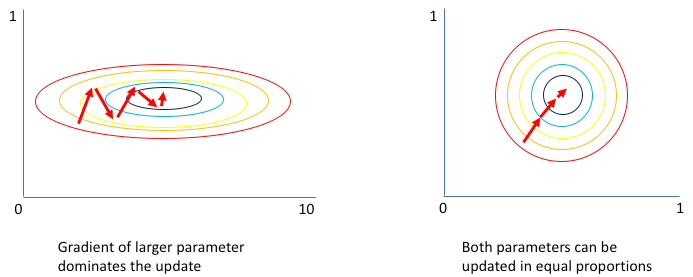
\includegraphics[width=120mm]{figs/Why_normalize.png}
\caption{Normalizing inputs to a standard scale}
\label{fig:normalize}
\end{figure}

Another factor influencing the convergence rate is the scaling of the input variables such that they have the same covariance, as inputs that have large variations in spread along different directions of the input space do also slow down the learning. 
This speeds up learning as it helps to balance out the rate at which the weights connected to input nodes learn. 
By normalizing each layer, we are introducing a level of orthogonality between layers - which generally makes it easier for the learning process.

\begin{figure}[ht]
\centering
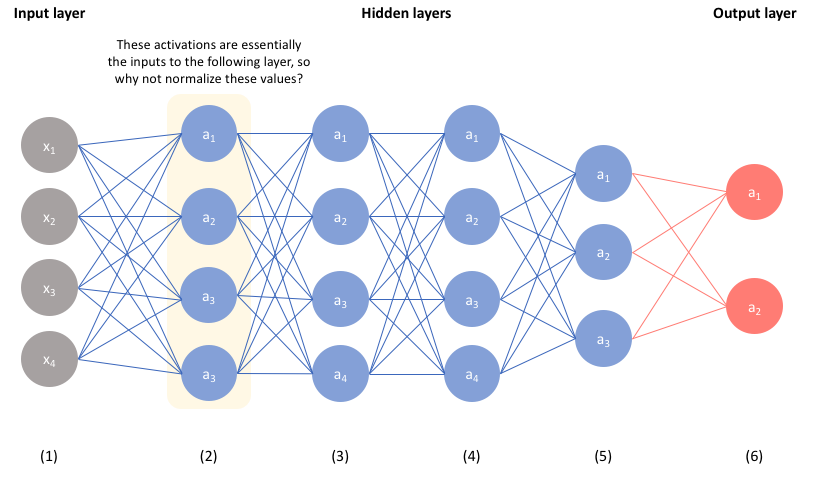
\includegraphics[width=120mm]{figs/Benefit of normalization.png}
\caption{Normalization on each layer}
\label{fig:normalize2}
\end{figure}

There is a module called batchnorm which is used for the same and is placed before or after ReLU or both for this purpose. 
It takes the sample of the batch and normalizes input values across the minibatch. 
In addition to batchnorm, there are alternative techniques - featurenorm and goodnorm - which address this problem. 
Feature norm normalizes across the entire feature and goodnorm normalizes across the entire array.
While training neural nets with gradient-based procedures, we adjust every weight according to its gradient under the assumption that other weights remain constant. 
However, they change every iteration in practice. Changes in weights in layer $k-1$ can result in a change of inputs to layer $k$. 
After applying batch norm to the layers, we make sure that the inputs to every layer are close to the standard normal distribution easing dependencies between layers. 
To increase the stability of a neural network, batch normalization normalizes the output of a previous activation layer by subtracting the batch mean and dividing by the batch standard deviation. 
Given a vector of linear combinations from the previous layer $z[l]$ for each observation $i$ in a dataset, we can calculate the mean and variance as: 
\begin{equation}
    \mu = \frac{1}{m} \sum_i z_i^{[l]}
\end{equation}
\begin{equation}
    \sigma^2 = \frac{1}{m} \sum_i (z_i^{[l]} - \mu)^2
\end{equation}
% μ=1/m∑i z_i^[l]
% σ2=1/m∑i z_i^[l]−μ)^2
Using these values, we can normalize the vectors $z[l]$ as follows.
% z_norm^(i)=(z(i)−μ)/√(σ^2+ε)
\begin{equation}
    Z_norm^(i) = \dfrac{z(i) - \mu}{\sqrt{\sigma^2+\varepsilon}}
\end{equation}
We add a very small number ϵ to prevent the chance of a divide by zero error.

Batch norm is the most popular however is not that great as it depends on the batch size and we need to maintain a running average of mean and standard deviation which can not be done when running on test cases and we need an equivalent operation for that time. 
In goodnorm, on the other hand, we do the same operation in both testing and training. 

As a result of introducing orthogonality between layers such that we avoid shifting distributions in activations as the parameters in earlier layers are updated, we can build deeper networks using normalization.

{\centering\fbox{\begin{minipage}{30em}
\centering\textbf{Normalize Input Variables}
\begin{enumerate}
    \item The mean of each input variable over the training set should be approaching zero.
    \item Scale input variables so that their covariances are about the same.
\end{enumerate}
\end{minipage}}\par}

% Authors: tn1050@nyu.edu, vy404@nyu.edu, sk7685@nyu.edu.
% Lecture date: 2.4.19
\section{Use a bit of L1 and L2 regularization on the weights} 
The use of regularization is well studied in the machine learning literature and they are used widely in different types of learning algorithms in one form or another to avoid overfitting. 
One form of regularization we can impose on the learning algorithm would be by putting constraints on the weights, and this is usually done by adding a term to the cost function. 
To that end, we can add 
\begin{equation}
\alpha*||w||_2^2 \hspace{0.5cm}
or \hspace{0.5cm}
\beta*||w||_1 
\end{equation}
terms to the cost function to impose L2 or L1 regularizations respectively. 
This will keep the model parameters from increasing and will increase the bias to ensure the model does not have high variance (i.e., overfitting). 
It will also help to remove some of the parameters if we use L1 regularization. 
Weight regularization also help the weights to spread around. 
That has some advantages for generalization as it tends to regularize the solution so that it is more general. 
It is best to start regularization after a couple of epochs and crank it up as loss decreases so that the solution does not collapse in the beginning with all weights becoming zero.

{\centering\fbox{\begin{minipage}{30em}
\centering\textbf{Use a bit of L1 and L2 regularization on the weights}
\begin{enumerate}
    \item It keeps the model parameters from increasing and will increase the bias to ensure the model does not have high variance.
    \item Best to start regularization after a couple of epochs else all weights become zero.
\end{enumerate}
\end{minipage}}\par}

% Authors: tn1050@nyu.edu, vy404@nyu.edu, sk7685@nyu.edu.
% Lecture date: 2.4.19
\section{Use “dropout” for Regularization}
Dropout is a way of regularization that makes neural nets more robust and prevents overfitting. 
It is a layer that randomly masks out some percentage of the units in the layer and “ignores” them during a particular forward or backward pass.

\begin{figure}[ht]
\centering
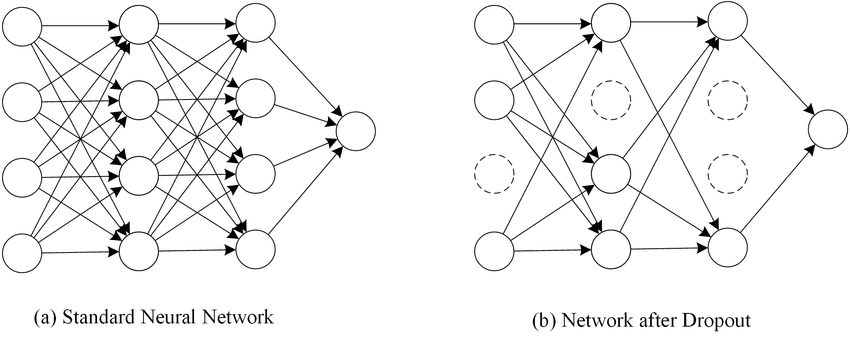
\includegraphics[width=120mm]{figs/Dropout.png}
\caption{Neural network dropout}
\label{fig:dropout}
\end{figure}

Dropout has the effect of making the training process noisy, forcing nodes within a layer to probabilistically take on more responsibility for the inputs. 
It helps to spread the evidence to multiple features and prevents the network from giving too much importance to a particular feature. 
It also provides a cheap way of ensembling multiple networks. 
Dropout also helps reduce interdependent learning amongst the neurons and limits the networks ability to memorize very specific conditions during the training. 
As we turn-off some of the hidden units (with some probability), the hidden units are less inclined to learn every redundant detail of instances in training set. 
The subsequent layers will have access to lesser details of the input instance, they increase their efficiency learning to find patterns for unseen data, which gives a boost in generalization.

Dropout may be implemented on any or all hidden layers in the network as well as the visible or input layer. It is not used on the output layer. 
A new hyperparameter is introduced that specifies the probability at which outputs of the layer are dropped out, or inversely, the probability at which outputs of the layer are retained. 
Dropout is not used after training when making a prediction with the fit network. 
The weights of the network will be larger than normal because of dropout. 
Therefore, before finalizing the network, the weights are first scaled by the chosen dropout rate. 
The network can then be used as per normal to make predictions.

{\centering\fbox{\begin{minipage}{30em}
\centering\textbf{Use “dropout” for Regularization}
\begin{enumerate}
    \item A layer that randomly masks out some percentage of the units in the layer and “ignores” them during a pass.
    \item Helps prevent the network from giving too much importance to a particular feature, and incentives to spread the evidence to multiple features
\end{enumerate}
\end{minipage}}\par}

% Authors: tn1050@nyu.edu, vy404@nyu.edu, sk7685@nyu.edu.
% Lecture date: 2.4.19
\section{Schedule To Decrease Learning Rate}
Some tricks are not well understood theoretically and are based on intuition supported by empirical evidence. 
One such trick is decreasing the learning rate during the training. 
When we observe the loss of the neural net plateaus and stops decreasing, it might be helpful to continue training with a lower learning rate. 

\begin{figure}[hbt!]
\centering
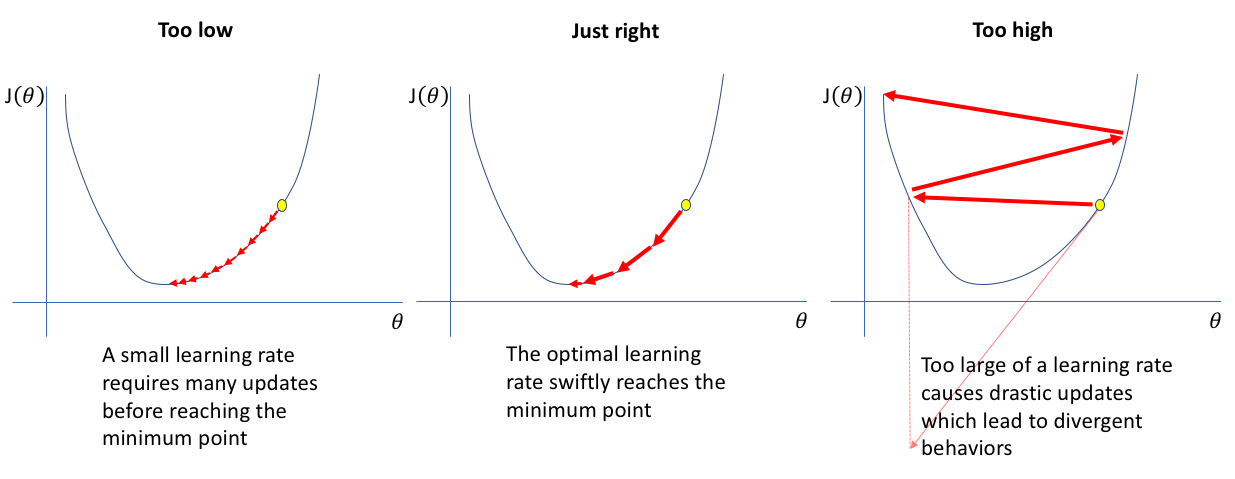
\includegraphics[width=120mm]{figs/Learning rate_3.png}
\caption{Gradient descent with small (left), optimal (middle) and large (right) learning rates}
\label{fig:learningrate1}
\end{figure}

To understand why this might be helpful, imagine there are two minima (one deep and narrow and another shallow and wider) and we are optimizing the model parameters with SGD.
Note that the noise in the gradients will be causing the parameters to fluctuate. 
The fluctuations will be smaller in the wider shallower minima than the narrow and deeper one as the weights will be bouncing off sharper in the narrower one, and they might bounce so much that the parameters will go out of the curvature. 
In the wider shallower minima it is very likely that the fluctuations will be smaller even though the minima is higher.

\begin{figure}[hbt!]
\centering
\begin{subfigure}{.5\textwidth}
  \centering
  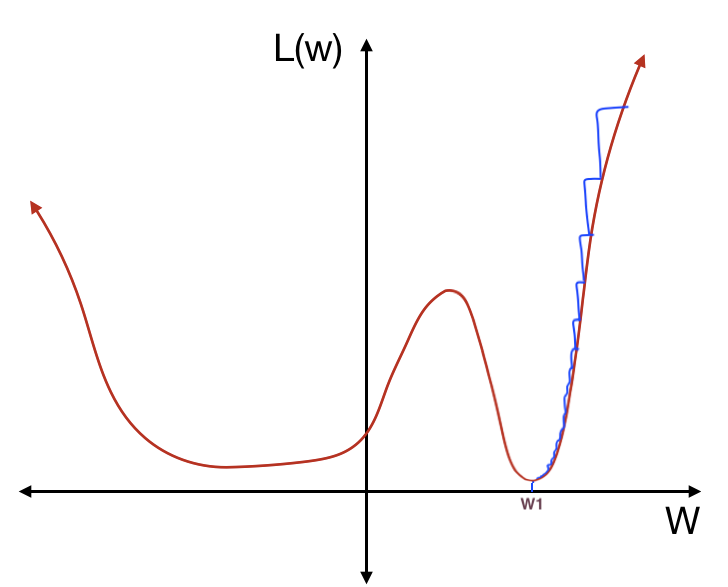
\includegraphics[width=.5\linewidth]{figs/Learning rate_1.png}
  \caption{}
  \label{fig:learningrateSub1}
\end{subfigure}%
\begin{subfigure}{.5\textwidth}
  \centering
  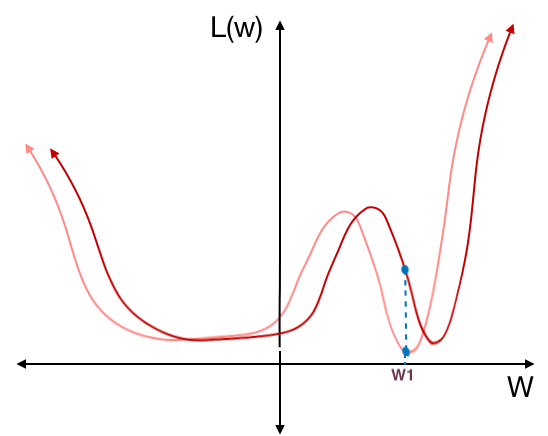
\includegraphics[width=.5\linewidth]{figs/Learning rate.png}
  \caption{}
  \label{fig:learningrateSub2}
\end{subfigure}
\caption{(a) Approaching a local minimum with changing step size (b) Slight shift in loss function resulting in a large change in loss}
\label{fig:learningrate2}
\end{figure}

Another thing to consider is that the average loss will be higher for the steeper minima than the shallower minima. 
When we stop the system at one point we might get a higher loss due to bouncing. 
For this reason, some people say that we should not use the last value of the parameters that we obtain through SGD and instead use the average of the past few values by keeping a running average. 
This will help us get closer to the minimum point of a steeper minima. 
This, however, does not guarantee a better test loss, as the loss function that we have in the test set would be different than that of the training set. 
Even if it has the same shape, it might be shifted by a bit. 
Such a shift would affect the loss value more if we are in a steeper minima point. 
One intuition is that we might have a regularization effect when the system wants to choose wider minima as it has a better chance of generalizing properly. 
Another intuition is that regardless of which minima you are in, if you want to get to it quickly, a large learning rate might help the system approach the minima but may not let it go inside the minima because of the large fluctuation and we need to decrease the learning rate so it can settle in the minima.

{\centering\fbox{\begin{minipage}{30em}
\centering\textbf{Schedule To Decrease Learning Rate}
\begin{enumerate}
    \item When the loss of the neural net plateaus, it might be helpful to continue training with a lower learning rate.
    \item Slight shift in loss function of test set results in a large change in loss.
\end{enumerate}
\end{minipage}}\par}
\vspace{5pt}

One reason why neural nets disappeared in the mid-90s was because of few people who had developed tricks to make neural nets run on their system however any people who tried new neural nets would not know them and would need to figure them out themselves. 
That led to people just giving up.  %backprogation in practice ch 6
\chapter{The Manifold Hypothesis}\label{chp: manifold_hypothesis}
% Authors: Hongyu (Florence) Lu, Michael Gold, Erica Dominic.
% Lecture date: 1.28.19

\section{Facial Expressions Thought Experiment}
% Authors: Hongyu (Florence) Lu, Michael Gold, Erica Dominic.
% Lecture date: 1.28.19

Say we have infinitely many pictures of a person making all possible facial expressions.
Each image is $2000 \times 1000$ pixels and has $3$ color channels, so each image is $6,000,000$-dimensional vector.

The set of all images is a small subset of $6,000,000$-dimensional space.
What does that subset look like?
What is the dimensions of the surface?
On a patch of that surface, how many dimensions can you move and still stay on that surface?

That surface is a manifold (roughly speaking, a continuous surface).
Moreover, it is limited by the number of degrees of freedom in the human face, which is bounded above by the number of muscle groups a person can control in his face.
Ergo that subset of $\mathbb{R}^{6000000}$ is relatively low-dimensional.

This thought experiment illustrates the manifold hypothesis, which postulates that natural data in high dimensional space generally has a low dimensional structure. %manifold hypo ch 31
\chapter{Tensor Transformations}
% Authors: Dustin Godevais , Reuben Juster, Yi Li,. 2/5/18.

The following sections summarize and visualize how you can transform data represented in matrix form. 
Input data can be defined as a matrix with the $i^{th}$ row corresponding to the $i^{th}$ data point and each additional columns representing a new dimension of the data.
$\matr{X}$ in the below examples is an input matrix with 1000 data points and two dimensions whose values are standard normally distributed. 
In the following figures, data points are colored according to their original $x_{N,1}$  dimension violet to yellow for negative to positive values.

\[
\matr{X} =
\begin{bmatrix}
    x_{1,1} & x_{1,2} \\
    x_{2,1} & x_{2,2} \\
    x_{3,1} & x_{3,2} \\
    \vdots & \vdots  \\
    x_{1000,1} & x_{1000,2}
\end{bmatrix}
\]

\begin{figure}[H]
\begin{center}
\includegraphics[width=200pt]{figs/standardnormal.png}
\end{center} 
\caption{Original $\matr{X}$ Visualized}
% \label{fig:mon}
\end{figure}

\section{Linear Transformations}
% Authors: Dustin Godevais , Reuben Juster, Yi Li,. 2/5/18.
There are several linear transformation that can be executed on $\matr{X}$ including:

\begin{itemize}
% \tightlist
\item
Rotation (\(\matr{U}\))

\item
Scaling \((s_1, s_2)\)

\item
Reflection (\(\matr{V}\))
\item
Shearing
\item
Translation
\end{itemize}

The product of the first three form weights as shown below.

\[
\matr{W} = \matr{U}
\begin{bmatrix}
    s_1 & 0 \\
    0 & s_2 
\end{bmatrix}
\matr{V}^\top
\]


\subsection{Rotation}
During rotation, each point is rotated about the origin by the indicated angle. 
The below equation populates $\matr{U}$ based on rotating points by \(\theta\) counter-clockwise.

\[
\matr{U} = 
\begin{bmatrix}
    \cos(\theta) & \sin(\theta)\\
    \sin(\theta) & -\cos(\theta)
\end{bmatrix}
\]

Keeping scaling and reflection constant, the below figure shows a set up points with different  \(\theta\)s .

\begin{figure}[H]
\begin{center}
\includegraphics[width=300pt]{figs/Rotation.png}
\end{center} 
\caption{Rotation Visualized}
% \label{fig:mon}
\end{figure}
% \FloatBarrier


\subsection{Scaling}
Scaling the points expands or contracts the points about the origin. 
This controlled separately for each dimension by \(s_1\) and \(s_2\) .

\begin{figure}[H]
\begin{center}
\includegraphics[width=300pt]{figs/Scaling.png}
\caption{Scaling Visualized}
% \label{fig:mon}
\end{center} 
\end{figure}
% \FloatBarrier


\subsection{Reflection}
Reflecting points projects them on the other side of a defined line that crosses the origin. 
The line that goes from the original point to the projected point is perpendicular to the defined line, and the intersection to the defined line is the midpoint.


\begin{figure}[H]
\begin{center}
\includegraphics[width=200pt]{figs/reflection_example.png}
\end{center} 
\caption{Reflection Defined}
% \label{fig:mon}
\end{figure}
% \FloatBarrier


\(\matr{V}\) can be defined by

\[
\matr{V} = 
\begin{bmatrix}
    \cos(2\theta) & \sin(2\theta)\\
    \sin(2\theta) & -\cos(2\theta)
\end{bmatrix}
\]

Where the defined line is \(x_2 = \tan(\theta) x_1 \)

\begin{figure}[H]
\begin{center}
\includegraphics[width=400pt]{figs/Reflection.png}
\end{center} 
\caption{Reflection Visualized}
% \label{fig:mon}
\end{figure}
% \FloatBarrier

\subsection{Shearing}
Shearing points, which is separate from the weight calculation, shifting points in one dimension proportional to their value in the other dimension.

\(\matr{Y} = \matr{X}  \begin{bmatrix}
    1 & k\\
    0 & 1
\end{bmatrix} \) 
Shift points on the \(x_1\) dimension proportional to the \(x_2\) dimension

\(\matr{Y} = \matr{X}  \begin{bmatrix}
    1 & 0\\
    k & 1
\end{bmatrix} \)
Shift points on the \(x_2\) dimension proportional to the \(x_1\) dimension

\begin{figure}[H]
\begin{center}
\includegraphics[width=400pt]{figs/shear.png}
\end{center} 
\caption{Shear Visualized}
% \label{fig:mon}
\end{figure}
% \FloatBarrier

\subsection{Translation}
The translation of points, which is separate from the weight calculations moves them uniforming in the direction indicated.

\[ \matr{Y} = \matr{X} 
+ \begin{bmatrix}
    1 & 1 \\
    1 & 1 \\
    1 & 1 \\
    \vdots & \vdots  \\
    1 & 1
\end{bmatrix}
\begin{bmatrix}
    t_1 & 0\\
    0 & t_2
\end{bmatrix} \] 
(Shift points left or right by \(t_1\) and up or down by  \(t_2\) dimension)

\begin{figure}[H]
\begin{center}
\includegraphics[width=400pt]{figs/translation.png}
\end{center} 
\caption{Translation Visualized}
% \label{fig:mon}
\end{figure}
% \FloatBarrier

\section{Non-Linear Transformations}
% Authors: Dustin Godevais , Reuben Juste, Yi Li,. 2/5/18.
Linear transformations are capable of altering data in many different ways, but linear transformations cannot curve data. 
That is where non-linear transformations come in. There are several types of non-linear transformations such as:

\begin{itemize}
% \tightlist
\item
Rectified linear unit (ReLU) - \(y = x_1\) if \(x_1 > 0\) else $0$ 
\item
Polynomial- \(y = x_1^2\) or \(y = x_1 x_2\)
\item
Step - \(y = 1\) if \(x > 0 \) else $0$ 

\end{itemize}

One of the most common non-linear transformations is the hyperbolic tangent, which in the context of 2D Tensors can be applied as below:
\[f(x) = \tanh(
\begin{bmatrix}
s & 0\\
0 & s
\end{bmatrix}
x)\]

This function first stretches out the points using scalar $s$ via scaling, then the hyperbolic tanget squashes the points into a square.
The larger $s$ is, the more points end up in the square.

\begin{figure}[H]
\begin{center}
\includegraphics[width=400pt]{figs/tanh.png}
\end{center} 
\caption{Tanh in Isolation}
% \label{fig:mon}
\end{figure}
% \FloatBarrier

Tanh can create curved surfaces when it is sandwiched in-between two linear transformations in a three layer neural network.

\begin{figure}[H]
\begin{center}
\includegraphics[width=400pt]{figs/tanh_sandwich.png}
\end{center} 
\caption{Tanh In-Between Two Linear Layers}
% \label{fig:mon}
\end{figure}
% \FloatBarrier
 % tensor transform ch 32
\chapter{Representation Learning}

\section{Introduction}
% Authors: 
% Lecture date: 4/22/2019
% Slides 1 - 6

Researchers have always been interested in learning about relations and interaction of components of networks and the motivation for it is what lots of science and knowledge is about. Like social science is about understanding how each component of the economy/society interact with each other i.e. Similarly in AI, researchers are interested in similar things. 

We can model these multi-relational data (relational knowledge) using entities + relationship model and use the model to do link prediction, entity resolution and community detection. 
\begin{figure}[htb!]
\centering
\includegraphics[width=0.5\linewidth]{figs/slides2.PNG}
\label{fig:tag_overlap}
\caption{Entities + relationship model}
\end{figure}
i.e Given the above graph, we can predict the link that Turning is also a citizen of UK which is not given by the data.

Researchers have been trying to build very large knowledge graph and they have been successful. Examples of them includes Google knowledge graph that contain 570 million nodes and over 18 billion edges. However, there are still problems with them like data still very noisy and incomplete despite the huge size.

One naïve but decently successful way to model knowledge graph is Markov Logic Model whose main idea is to combine graphical models with probability inference. We can give probability inference based on rules given. However, there are two major problems for this model: scalability and requirement of prior knowledge.

% Slides 6 -  (for reference)
Slides 6-7:
The main idea of embedding model is to extract feature representation to explain relationship and is the formula inspired by NLP embedding i.e we can add embedding of man and women to get close to man.
However, there is problem wrt the formula (TransE) which is the symmetric relationship
F(s,p,o) != f(o,p,s)

Slides 8-9:
The way to fix the problem is to use dot product (RESCAL)
It’s equivalent to factorize a large adjacency matrix to two matrix of relationships
We explained relationship via interactions of latent features

Slides 10:
This model is good that it has decoupling effect. It gives the property that makes the model scalable.
The model is differentiable and can use gradient optimization 
Need minimal prior knowledge, only need some observation and scoring function.

Slides 11:
Task: learn to find out test countries belong to which region.
We know train belong to sub belongs to region.
Can apply to much larger and complex problems

Slides 12:
However, in the example, it seems we haven’t reached saturated point, but increasing dimensionality would make computation too hard.

Slides 13:
Lots of knowledge have underlying hierarchical structure 

Slides of 14:
Example of the tree like structure
Number of nodes grow exponentially with depth
Volume of embedding space will need to grow very fast

%%%%%%%%%%%%%%%%%%%%%
%% Begin Sreyas' part

%% Kevin writes until 37 minutes in the video. Assumes that Kevin has written the equations for score function and probabilistic mdoel. 

%%start time 36 minutes
\subsection{TransE}
TransE introduced by Bordes et al. 2013 uses a score function of the form $$ f(s, p, o) = -|| e_s + r_p - e_o ||_p $$ where $e_i$ are entity and $r_i$ are relational embedding. Note that is is basically saying that if you take the embedding of $o$ and add the embedding of relationship, you should be close to the embedding of $p$ - this is very similar to what we see in word2vec. 

This score function is particularly nice in the sense that this is very fast to compute, the running time is $\mathcal{O}(d_e)$ where $d_e$ is the embedding dimension. A particularly stricking problem with the cost function is it's inability to model symmetric relations. A relation $p$ of the form $f(s, p, o) = f(o, p, s)$ for all $s, p$ is called a symmetric relation. Note that, if $f(s, p, o) = f(o, p, s)$ is satisfied, then this implies that $r_p$ should be zero vector. Therefore, one can model only one symmetric relation using this formalism. 

\subsection{RESCAL}
RESCAL introduced by Nickel et al, 2011 uses a cost function of the form:
$$ f(s, p, o) = e_s^TRpe_o$$
Note that, unlike TransE, relational embeddings have a different size from entity embedding and we see it as a matrix. This score function takes $\mathcal{O}(d_e^2)$ making it's evaluation difficult in large graphs. 

One could think about the components of entity embedding as latent features of the entities. Note that 
$$  f(s, p, o) = e_s^TRpe_o = r_p^T(e_s \mathop{\otimes} e_o) $$ where $(e_s \mathop{\otimes} e_o)$ represents the outer product of $e_s$ and $e_o$. $(e_s \mathop{\otimes} e_o)$ may be thought of as representing a feature vector for the pair $(e_s, e_o)$ and then applying it to a linear classified with weight $r_p$ gives as the score $f(s, p, o)$

\subsection{Discussion on Relational Learning with Embedding}
\begin{figure}[htb!]
\centering
\includegraphics[width=0.5\linewidth]{figs/relational_learning_graphical_model.png}
\label{fig:relational_learning_gm}
\caption{Graphical Model Representing Relational Learning with Embedding}
\end{figure}

Figure \ref{fig:relational_learning_gm} shows the graphical model capturing dependencies of relational learning with embedding. Some of the merits of this method are:
\begin{enumerate}
    \item \textbf{Decoupling} Unlike Markov Logic Networks, one can using do inference by doing a local computation $f(s, p, o)$
    \item \textbf{Gradient Based Optimization} The loss function is differential and the score functions $f(s, p, o)$ are also typically differentiable, which means one can use gradient based methods for learning helping to scale up easily to large datasets.
    \item \textbf{Minimal Prior Knowledge} Unlike Markov Logic Network, one need not have any prior knowledge about the problem - one can easily learn them in this framework. 
    \item \textbf{Black Box Model} Less interpretable than MLN.
\end{enumerate}


%% Ended at 01:00:00 
%% Have to write from Poincare Embedding or Hierarchical Structures and Representation Learning

%% End of Sreyas' part
%%%%%%%%%%%%%%%%%%%%%%%%%%


\section{Hierarchical representation in Hyperbolic Space}
Representation learning has become an invaluable approach for learning from symbolic data such as text and graphs. However, while complex symbolic datasets often exhibit a latent hierarchical structure, state-of-the-art methods typically learn embeddings in Euclidean vector spaces, which do not account for this property.

For example, in a tree-like graph structure, we aim to embed nodes such that the distance between the nodes is less than a given distance ‘r’ if they are connected and greater than ‘r’ otherwise.

\begin{figure}[htb!]
\centering
\includegraphics[width=0.5\linewidth]{figs/tree_graphs.PNG}
\label{fig:treegraphs}
\caption{Tree-like graphs with embedded nodes having distance less than 'r' if connected and greater than 'r' otherwise}
\end{figure}

But the problem with the tree-like structure is the number of nodes grows exponentially with depth. Thus, as the radius of the graph increases, to maintain the above-mentioned rule for distance, the volume needs to also grow exponentially. This exponential growth of volume is not possible in Euclidean space thus the only possible way to address this need for exponential growth is through increasing the dimensionality. The limitations with increasing the dimensionality are 1) its expensive in terms of memory for computation 2) it only conserves topology/structure rather than semantics, which is of actual importance for our model learning.
\begin{figure}
\centering
\includegraphics[width=0.5\linewidth]{figs/tree_graphs_limitation.PNG}
\label{fig:tree_graphs_limitation}
\caption{Limitation of representation of tree-like graphs in Euclidean Space when the depth increases.}
\end{figure}


A better way for geometric representation of a tree-based graph is by calculating the similarity in hyperbolic space rather than the Euclidean space. The geometrical properties which make hyperbolic space more suitable for this task are 1) It is a continuous analog of trees 2) It acts as geometric prior for hierarchies 3) it is still a Riemann manifold which enables the use of gradient-based optimization to compute embeddings.

\subsection{Poincaré Embeddings for
Learning Hierarchical Representations}

The most intuitive example of hyperbolic space for representation learning is the Poincare Ball Model. Poincare Ball Model is a new approach for learning hierarchical representations of symbolic data by embedding them into hyperbolic space – or more precisely into an n-dimensional Poincaré ball. Due to the underlying hyperbolic geometry, this allows learning parsimonious representations of symbolic data by simultaneously capturing hierarchy and similarity.

\begin{figure}[htb!]
\centering
\includegraphics[width=0.5\linewidth]{figs/poincareball_semantics.PNG}
\label{fig:poincareball_semantics}
\caption{Modelling Semantics in Poincare Ball Model}

\end{figure}

For modeling tree-like structure in the Poincare ball 1) the roots are points at the origin which are relatively close to all points 2) leaves are points at the boundary which are far apart from most of the points 3) the shortest paths are the geodesics which go through more general points.

\begin{figure}[htb!]
\centering
\includegraphics[width=0.5\linewidth]{figs/poincareball_geodesics.PNG}
\label{fig:poincareball_geodesics}
\caption{Geodesics in Poincare Ball Models}
\end{figure}

\chapter{Relational Learning with Embeddings}

\section{Poincaré Embeddings}

% Authors: Manrique Vargas, Aakriti Gupta, HuiYu Sun
% Part 2
% Lecture date: 4/22/2019

\subsection{Introduction}
We introduce hierarchical representations of symbolic data by embedding them into hyperbolic space – an n-dimensional Poincaré ball. The underlying hyperbolic geometry allows us to learn representations of symbolic data by simultaneously capturing hierarchy and similarity\cite{NIPS2017_7213}. The underlying hyperbolic geometry allows us to learn representations of symbolic data by simultaneously capturing hierarchy and similarity. We present an efficient algorithm to learn the embeddings based on Riemannian optimization and show experimentally that Poincaré embeddings can outperform Euclidean embeddings significantly on data with latent hierarchies, both in terms of representation capacity and in terms of generalization ability .

\subsection{Poincaré Model of Hyperbolic Space}

Poincaré Model of Hyperbolic Space can embed data such that the distance in the embedding space reflects their semantic similarity. It assumes that there exists a latent hierarchy in which the symbols can be organized. In addition to the similarity of objects, it intends to reflect this hierarchy in the embedding space to improve over existing methods in two ways:
\begin{itemize}
    \item Incorporate an appropriate structural bias on the embedding space to improve generalization performance, run time, and memory complexity.
    \item Capture the hierarchy explicitly in the embedding space to gain additional insights about the relationships between symbols and the importance of individual symbols.
\end{itemize}

The model considers the task of inferring the hierarchical relationships fully unsupervised, as is, for instance, necessary for text and network data. In contrast to Euclidean space $ \mathbb{R}$, there exist multiple, equivalent models of $ \mathbb{H}$ such as the Beltrami-Klein model, the Hyperboloid model, and the Poincaré half-plane model. 

Poincaré ball model is well-suited for gradient-based optimization. In particular, assume a Riemannian manifold $(B_d , d_p )$ where  $B_d = {x \in \mathbb{R}_d | \norm{x} < 1}$ is the open d-dimensional unit ball, where $\norm{}$ denotes the Euclidean norm. The distance between points $\Vec{u}$, $\Vec{v} \in B_d$ is given as:

\begin{equation} \label{eq:poincarredistance}
    d_p(\Vec{u},\Vec{v})= arcosh(1+2 \dfrac{\norm{\Vec{u}-\Vec{v}}^2}{(1-\norm{\Vec{u}}^2)(1-\norm{\Vec{v}}^2)})
\end{equation}

 The boundary of the ball is denoted by ∂B. It corresponds to the sphere S d−1 and is not part of the manifold, but represents infinitely distant points. Geodesics in B d are then circles that are orthogonal to $\delta B$ (as well as all diameters). See ~\ref{fig:poincaredisk} and ~\ref{fig:poincaregrowthdist} for an illustration.

It can be seen from Equation ~\ref{eq:poincarredistance}, that the distance within the Poincaré ball changes smoothly with
respect to the location of u and v. This adds a locality property to amplify the Euclidean distance. This locality property of the Poincaré distance is key for finding continuous embeddings of hierarchies. For example, by placing the root node of a tree at the origin of $B_d$ it would have a relatively small distance to all other nodes as its Euclidean norm is zero. On the other hand, leaf nodes can be placed close to the boundary of the Poincaré ball as the distance grows very fast between points with a norm close to one. Furthermore, please note that Equation ~\ref{eq:poincarredistance} is symmetric and that the hierarchical organization of the space is solely determined by the distance of points to the origin. Due to this self-organizing property, Equation ~\ref{eq:poincarredistance} is applicable in an unsupervised setting where the hierarchical order of objects is not specified in advance such as text and networks.

Equation ~\ref{eq:poincarredistance} allows us therefore to learn embeddings that simultaneously capture the hierarchy of objects (through their norm) as well a their similarity (through their distance). Since a single hierarchical structure can be well represented in two dimensions, the Poincaré disk ($ \mathcal{B}^2 $) is a common way to model hyperbolic geometry. The Poincaré ball ($ \mathcal{B}_d $) is used for two main reasons: first, in many datasets such as text corpora, multiple latent hierarchies can co-exist, which can not always be modeled in two dimensions. Second, a larger embedding dimension can decrease the difficulty for an optimization method to find a good embedding (also for single hierarchies) as it allows for more degrees of freedom during the optimization process. 

It can be seen that geodesics also have shortest paths through more general points. In addition, modelling tree structures in the Poincaré ball allows us to represent roots of the trees since points at the origin are relatively close to all points, and represent leafs as points at the boundary are far apart from most points. 
This gives us an exponential volume growth to model our distance.

\begin{figure}[htb]
    \begin{center}
    \begin{subfigure}[b]{0.3\textwidth}
    \includegraphics[width=\textwidth]{figs/1-1-1.png}
        \caption{Geodesics of the Poincaré disk}
        \label{fig:poincaredisk}
    \end{subfigure}
    \begin{subfigure}[b]{0.29\textwidth}
        \includegraphics[width=\textwidth]{figs/1-2.png}
        \caption{Growth of Poincaré distance}       
        \label{fig:poincaregrowthdist}
    \end{subfigure}
    \caption{(a) Due to the negative curvature of B, the distance of points increases exponentially (relative to their Euclidean distance) the closer they are to the boundary. (b) Growth of the Poincaré distance $d(u, v)$ relative to the Euclidean distance and the norm of v (for fixed $\norm{u} = 0.9)$.(b) Embedding of a regular tree in $\mathcal{B} ^2$ such that all connected nodes are spaced equally far apart (i.e., all black line segments have identical hyperbolic length).}\label{fig:poincarreilus}
    \end{center}
\end{figure}

\subsection{Large Scale Embedding via Rieminian Representation}
\title{Optimization}

To compute Poincaré embeddings for a set of symbols $S = {x_i}_i^n =1$ , we are then interested in finding
embeddings $\theta = {\big\{ \theta_i\big\}}_{i=1}^n$, where $\theta_i \in  \mathscr{B}^2$ . We assume we are given a problem-specific loss function $\mathcal{L}(\theta)$ which encourages semantically similar objects to be close in the embedding space according to their Poincaré distance. To estimate $theta$, we then solve the optimization problem
\begin{equation} \label{eq:poincarresdg}
    \theta \xleftarrow{} argmin_\theta   \mathcal{L}(\theta)  s.t. \forall  \theta_i \in \theta : \norm{\theta_i} < 1
\end{equation}

As we are not in Euclidean space, we cannot use conventional stochastic gradient decent. Since the Poincaré Ball has a Riemannian manifold structure, we can optimize Equation ~\ref{eq:poincarresdg} via stochastic Riemannian optimization methods. In particular, let $\mathscr{T_\theta B}$ denote the tangent space of a point $\theta \in \mathscr{B}_d$. Furthermore, let $\nabla_\mathcal{R} \in  \mathscr{T_\theta B}$ denote the Riemannian gradient of $\mathcal{L}(\theta)$ and let $\nabla E$ denote the Euclidean gradient of $\mathcal{L}(\theta)$. Using RSGD \cite{6487381}, parameter updates to minimize Equation ~\ref{eq:poincarresdg} are then of the form:
\begin{equation} \label{eq:poincarresdg2}
    \theta_{t+1} = EXP_{\theta_t} (−\eta_t \nabla_R \mathcal{L}(\theta_t))
\end{equation}
For the minimization of Equation ~\ref{eq:poincarresdg2} we require the Riemannian gradient and a suitable retraction. Since the Poincaré ball is a conformal model of hyperbolic space, the angles between adjacent  vectors are identical to their angles in the Euclidean space. The length of vectors however might differ. To derive the Riemannian gradient from the Euclidean gradient, it is sufficient to rescale $nabla_E$ with the inverse of the Poincaré ball metric tensor, i.e. $g_/theta^{−1}$. Since $g_/theta$ is a scalar matrix, the inverse is trivial to compute. In particular, the Euclidean gradient $\nabla_E$ depends on the gradient of $\frac{\delta \mathcal{L}(\theta)}{\delta(\theta x}$, which we assume is known, and the partial derivatives of the Poincaré distance $\frac{\delta(\theta, x)}{\delta\theta}$.

Therefore we obtain the Reimannian gradient from the Euclidean gradient in the form:
\begin{equation} \label{eq:riemanniangrad}
    \nabla_{R} = g_{\theta}^{−1}\nabla_{\epsilon} = \dfrac{(1−\norm{\theta_t^2})^2}{4} \nabla_{\epsilon}
\end{equation}

Furthermore, since Equation ~/ref{eq:poincarredistance} is fully differentiable, the Euclidean gradient can easily be derived. As retraction operation, we use $Exp_{\theta}(\vec{x}) = \theta + \vec{v}$. 

Reimannian manifold has an associated Euclidean tension space. The exponential map takes the point on the tension space and takes it back to the manifold.

In summary, the full update for a single embedding is then of the form:
\begin{equation} \label{eq:riemmaniansdg}
        \theta_{t+1}  \xleftarrow{} proj \bigg(\theta_t - \eta_t\dfrac{(1−\norm{\theta_t^2})^2}{4} \nabla_E \bigg)
\end{equation}

It can be seen from that this algorithm scales well to large data-sets, as the computational and memory complexity of an update depends linearly on the embedding dimension. This model allows us to embed graphs with millions of nodes and billions of edges on a single machine.

\subsection{Evaluation of Poincare Embedding}
\subsubsection{Embedding Latent Taxonomies}

WORDNET is a lexical database that among-st others, captures hypernym relations, i.e.: 'Tiger is-a Big cat'. Embeddings trained on WORDNET provide state-of-the-art performance for lexical entailment. On collaboration networks, we show that Poincaré embeddings are successful in predicting links in graphs where they outperform Euclidean embeddings, especially in low dimensions.  

Assuming that the latent hierarchy is embedded, we can recover the latent hierarchy from indirect obfuscated graph. This way we recover the expected taxonomies and materialize the relationships. See ~\ref{fig:wn-nouns} for an illustration.
\begin{figure}[htb]
  \centering
    \includegraphics[width=\textwidth]{figs/wn-nouns2.jpg}
    \caption{Embedding Latent Taxonomies}
    \label{fig:wn-nouns}
\end{figure}

\subsubsection{Historical Linguistics}
Historical linguistics refer to the study of languages relations and origins. Cognates are words that are shared across different languages we assume that they indicate common entities. This example illustrates the embeddings of language in hyperbolic space. Embeddings were clustered into different language families (Roman, Germanic, Indo-European, Greek, etc.) and distance from the origin captures historical relationships. See figure  (~\ref{fig:liguistics}) for an illustration.
\begin{figure}[htb]
    \begin{center}
    \begin{adjustbox}{minipage=0.5\textwidth,scale=0.5}
    \begin{subfigure}[b]{\columnwidth}
        \includegraphics[width=\textwidth]{figs/1-4.png}
            \caption{Intermediate embedding after 20 epochs}
            \label{fig:linguistics1}
        \vspace{0.7cm}
        \end{subfigure}
        \begin{subfigure}[b]{\columnwidth}
            \includegraphics[width=0.5\textwidth]{figs/1-5.png}
            \caption{Embedding after convergence}       
            \label{fig:linguistics2}
        \end{subfigure}
    \end{adjustbox}
    \caption{Two-dimensional Poincaré embeddings of transitive closure of the WORDNET mammals sub tree. Ground-truth is-a relations of the original WORDNET tree are indicated via blue edges. A Poincaré embedding with d = 5 achieves mean rank 1.26 and MAP 0.927 on this subtree).}\label{fig:liguistics}
    
    \end{center}
\end{figure}

In the first set of experiments, we are interested in evaluating the ability of Poincaré embeddings to embed data that exhibits a clear latent hierarchical structure. For this purpose, Maximilian Nickel and Douwe Kiela \cite{NIPS2017_7213} conduct experiments on the transitive closure of the WORDNET noun hierarchy in two settings:
\begin{itemize}

    \item \textbf{Reconstruction.} To evaluate representation capacity, they embed fully observed data and reconstruct it from the embedding. The reconstruction error in relation to the embedding dimension is then a measure for the capacity of the model.
    \item \textbf{Link Prediction.} To test generalization performance, they split the data into a train, validation and test set by randomly holding out observed links. The validation and test set do not include links involving root or leaf nodes as these links would either be trivial or impossible to predict reliably.
\end{itemize}

Embedding based on the Poincaré distance are compared with two distance function models: Euclidean and Translational. Results are shown in table ~\ref{table:table-comparisons}:

\begin{table}[htb]
  \centering
    \includegraphics[width=\textwidth]{figs/1-3.png}
    \caption{Experimental results on the transitive closure of the WORDNET noun hierarchy. Highlighted cells indicate the best Euclidean embeddings as well as the Poincaré embeddings which achieve equal or better results. Bold numbers indicate absolute best results}
    \label{table:table-comparisons}
\end{table}

It can be observed from table  ~\ref{table:table-comparisons} that hyperbolic Poincaré embeddings achieve much more efficient representation for low dimensions. 

\section{Lorentz Model of Hyperbolic Space}

There are multiple equivalent models of hyperbolic space (e.g. Minkowski, Poincare, Beltram, Klein) and we can map freely between them. Lorentzian Scalar Product is an example convenient to optimize:
\begin{equation} \label{eq:riemmaniansdg3}
         \langle \vec{u},\vec{v} \rangle = -v_0 u_0 + \sum_n v_n u_n
\end{equation}  
The Hyperboloid space 
\begin{equation} \label{eq:riemmaniansdg4}
         \mathbb{H}_n = {x \in \mathbb{R}_{n+1}:\langle \vec{u},\vec{v} \rangle_{ \mathcal{L}}= -1, x_0 > 0 }
\end{equation}  
The Lorentz model of Hyperbolic space is the Riemannian manifold  $\mathcal{L}^n =  \mathbb{H}_n , d_{\mathbb{l}}$
where Lorentz distance is defined as $d(\vec{u},\vec{v}) = arccos (-\langle \vec{u},\vec{v} \rangle_{ \mathcal{L}}) $

\section{Latent Space Semantics}

We use a lot of embeddings in Euclidean space to model structures but not semantics. We want our latent features to have proper semantics. Reasoning and semantics in euclidean space require a semantically coherent space where the probability distribution should be meaningful in our geodesic space.  

 Consider a logarithmic map that provides a direction in a particular length:
 $l(\vec{u},\vec{v},\sigma)= Exp_{\vec{u}} log_{\vec{u}}\vec{v}$.
 
 For example, for the relationship of mammals embedding taking steps along a linear interpolation. The nearest neighbor in euclidean space is shown below:
\begin{itemize}
    \item Golden Retriever
    \item Chesapeake Bay Retriever
    \item Blue Point Siamese
    \item Burmese Cat
\end{itemize}

Meanwhile, the nearest neighbor in hyperbolic space has more semantic structure:
\begin{itemize}
    \item Golden Retriever
    \item Carnivore
    \item Mammal
    \item Feline
    \item Burmese Cat
\end{itemize}

Similarly, another example within the mammals embedding space between mountain goat and pygmy sperm whale:
\begin{itemize}
    \item Mountain Goat
    \item Ungulate
    \item Grampus
    \item Pygmy Sperm Whale
\end{itemize}

Meanwhile, the nearest neighbor in hyperbolic space has more semantic structure going through subclass of aquatic mammals:
\begin{itemize}
    \item Mountain Goat
    \item Ungulate
    \item Mammal
    \item Cetacean
    \item Pygmy Sperm Whale
\end{itemize}

It can be observed that the hyperbolic space captures the semantics of taxonomies much better.


\section{Challenges}

\subsection{Riemannian Optimization}

In Euclidean space, we have a bunch of tools to do optimization really efficiently, ranging from Stochastic Gradient Descent (SGD) to second order optimization. However, in Riemannian manifolds, optimization tools are much less developed than in Euclidean space. There are many challenges involved. The main tool in use that works is the Riemannian Stochastic Gradient Descent proposed by Bonnabel in 2013. Parameter updates are given by the following equation:

\begin{equation} \label{eq:RSGD}
    \theta_{t+1} = EXP_{\theta_t} (−\eta_t \nabla_R \mathcal{L}(\theta_t))
\end{equation}

\begin{figure}[htb]
  \centering
    \includegraphics[width=0.4\textwidth]{figs/1-Lorentz.png}
    \caption{Lorentz model of hyperbolic geometry}
    \label{fig:1-Lorentz}
\end{figure}

But the problem with this is that the optimization is sometimes tricky to get right so people often resort to using small batch sizes, which results in slow convergence and the model will get stuck in local mini-ma. One way to improve these tools is to develop optimization methods in many manifolds that work significantly better than what we have now.

The Lorentz model in figure (~\ref{fig:1-Lorentz}) proposed by (Nickel et. al., 2018) showed good improvements over the Poincare disk. And advanced methods such as the RSVRG proposed by (Zhang et. al., 2016) didn't show significant gains for embeddings.  

\subsection{Methods}

Another important thing to think about conceptually is that if we switch the geometry, we now can not use easily our standard machine learning to do the task. A lot of benefits that we typically have from embedding is that they are intrinsic to relation-learning. Take word embeddings for example. The problem is that the standard machine learning, especially deep learning frameworks they all make this assumption. So you can't expect to just put the embeddings in and expect them to do something. So how can we make these embeddings usable? Is there some kind of translation we can adapt.

Researchers have found that using Riemannian manifolds in latent spaces for generative models is very promising as explored by Davidson et. al., 2018, as shown in figure (~\ref{fig:2-Davidson}). However, they have also been widely used in natural language understanding in downstream tasks. But a majority of machine learning and deep learning makes the Euclidean assumption.

\begin{figure}[htb]
  \centering
    \includegraphics[width=0.2\textwidth]{figs/2-Davidson.png}
    \caption{Riemannian manifolds for generative models is very promising}
    \label{fig:2-Davidson}
\end{figure}

\subsection{Embedding and Cognitive Science}

In cognitive science, the human similarity judgments are often non-metric. The classic example is that if you ask a human whether a man is similar to a centaur as depicted in figure (~\ref{fig:3-cog}), they will say yes. And if ask a human whether a centaur is similar to a horse, they will also say yes. However, if we ask a human whether a horse is similar to a man, they will say no. And it is a very strongly no. The problem with this is that if we have a very strong disagreement in these similarity judgments, it conflicts with the triangle inequality, which says: 

\begin{equation} \label{eq:triangleIne}
    d(u,v) \leq d(u, w) + d(w, v)
\end{equation}

This means that we won't be able to embed these similarity judgments properly. In this case, we need to think about non-metric measures. But this opens another can of worms.

\begin{figure}[htb]
  \begin{center}
    \includegraphics[width=0.8\textwidth]{figs/3-cog.png}
    \caption{The human similarity judgment experiment in cognitive science}
    \label{fig:3-cog}
    \end{center}
\end{figure}

\subsection{Tools}

Hype is an open source library to embed graphs into hyperbolic space. It can be used to play with these models. It is a Pytorch-based embeddings framework and supports Hyperbolic, Euclidean and Spherical manifolds. It is available on github via the following link:

http://github.com/facebookresearch/poincare-embeddings.


\section{Summary}

Christopher Strachey in a letter to Alan Turing summarized the utilization of relations  between data entities and their applications to Logical, analogical, taxonomical and knowledge bases.


\begin{itemize}
    \item Relational embeddings provide high-quality models of large-scale relational data.
    \item Graph neural networks learn inductive models of graph-structured data.
    \item Geometry of the embedding space acts as a prior on the structure of similarity relations.
    \item Hyperbolic embeddings are used to capture similarity and hierarchy in symbolic data
\end{itemize}

\chapter{Sparse Coding}
% Authors: Francesco Preta (Editor), Ambuj Ojha (Part1), Bingqian Deng (Part2)
% Lecture  date: 4/29/2019 part 1


%Beggining of Bingqian's part
\section{Energy-Based Unsupervised Learning}
Unsupervised learning can be approached through the optimization of an energy function. In order to do so, we need to model such function following a set of rules:
\begin{enumerate}
    \item Build the machine so that the volume of low energy stuff is constant;
    \item Push down of the energy of data points, push up everywhere else;
    \item Push down of the energy of data points, push up on chosen locations;
    \item Minimize the gradient and maximize the curvature around data points;
    \item Train a dynamical system so that the dynamics goes to the manifold;
    \item Use a regularizer that limits the volume of space that has low energy;
    \item If $E(Y) = ||Y - G(Y)||^2$, make $G(Y)$ as "constant" as possible;
    \item Adversarial training: generator tries to fool real/synthetic classifier.
\end{enumerate}% \begin{figure}[h!]
% \centering
% \includegraphics[width=1.0\linewidth]{19_ss_a.png}
% \caption{Daily productive hours: Feb.18 $\sim$ Apr.4 2019}
% \label{fig:dailyhour}
% \end{figure}


In particular, the main focus of the lecture will come from the sixth point, using sparse coding, sparse auto-encoders and Predictive Sparse Decomposition (PSD).

\subsection{The Decoder with Restricted Latent Variable Model}

In what follows, we will use the following notation: $Z$ is the latent variable, possibly high dimensional, $Y$ is the observed signal, $Y'$ is the prediction signal reconstructed through a decoder. Such reconstruction can be obtained by matrix multiplication or through a neural network in more sophisticated models. The mathematical formulation is as follows : 
\[Y'=\operatorname{Dec}(\mathbf{Z}) \quad \mathbf{Z}^{*}=\operatorname{argmin}\|Y-\operatorname{Dec}(\mathbf{Z})\|+R(\mathbf{Z})\]
When given the target, the goal is to find the latent $Z$ that minimizes the energy function. This has generally two terms, one is the residual error (the difference between the prediction and target) and the other is the regularizer on $Z$, which restricts the space in which we can find the optimum and increases regularity of the solutions. In sparse coding, the regularizer is usually the $L^1$ norm of $Z$, which has the effect of setting to zero most of the components. Fig. \ref{fig:decoder} shows the structure just described, while Fig.\ref{fig:energy} shows different types of energy functions.
\begin{figure}[H]
\centering
\includegraphics[width=1.0\linewidth]{figs/decoder.png}
\caption{The Decoder with Restricted Latent Variable Model}
\label{fig:decoder}
\end{figure}
\begin{figure}[H]
\centering
\includegraphics[width=0.8\linewidth]{figs/ernergy.png}
\caption{Energy Functions of Various Methods}

\label{fig:energy}
\end{figure}
\section*{Sparse Coding and Sparse Modeling}

Fig \ref{fig:sparse} shows the scheme of sparse linear reconstruction \cite{olshausen1997sparse}, while fig \ref{fig:generative} shows the framework of performing inference in generative models.
The energy function is modeled as follows:
\[E\left(Y^{i}, Z\right)=\left\|Y^{i}-W_{d} Z\right\|^{2}+\lambda \sum_{j}\left|z_{j}\right|\]
\begin{figure}[H]
\centering
\includegraphics[width=1.0\linewidth]{figs/generative.png}
\caption{Inference in a Generative Model}
\label{fig:generative}
\end{figure}

\begin{figure}[H]
\centering
\includegraphics[width=1.0\linewidth]{figs/sparse.png}
\caption{Sparse Coding}
\label{fig:sparse}
\end{figure}
$W_d$ is called the dictionary matrix, where the first term represents the reconstruction error and the second term deals with the sparsity. However, the optimization algorithm to find $Z$ for a fixed $Y$ is computationally expensive. The algorithm that deals with auto-encoding and the regularizer term is called ISTA (Iterative Shrinkage Threshold Algorithm). 

Fig \ref{encoder} shows the encoder architecture. Most ICA models and Product of Experts are examples of this architecture.

\begin{figure}[H]
\centering
\includegraphics[width=1.0\linewidth]{figs/encoder.png}
\caption{Encoder Architecture}
\label{encoder}
\end{figure}
Fig \ref{enco_deco} shows the encoder-decoder architecture. The input $Y$  is passed through a feed-forward model, possibly with a regularizer, to make a prediction for the code. Once the coding is done, we pass the result through the decoder and measure the reconstruction error. An example of regularized auto-encoder is given by the Variational Auto-encoder, a model which uses noise rather than $L^1$ norm sparsity to reduce the information content.

\begin{figure}[H]
\centering
\includegraphics[scale=0.4]{figs/enco_deco.png}
\caption{Encoder-Decoder Architecture}
\label{enco_deco}
\end{figure}

The reason why the information content of the code has to be reduced is because otherwise the learning is not successful. In fact, when trained by minimizing the reconstruction error over the training set without any additional component, the algorithm does not learn structure from training sample, but rather it copies the data. Reducing the number of available features forces the algorithm to understand the underlying structure, which is why we reduce dimensions or introduce sparsity. Fig. \ref{code2} and Fig. \ref{reduce} give a graphical representation of such mechanism.

\begin{figure}[h]
\centering
\includegraphics[width=1.0\linewidth]{figs/code2.png}
\caption{Encoding without reducing the number of features}
\label{code2}
\end{figure}

\begin{figure}[h]
\centering
\includegraphics[width=1.0\linewidth]{figs/reduce_code.png}
\caption{Encoding while reducing the number of available features.}
\label{reduce}
\end{figure}


\subsection{Predictive Sparse Decomposition (PSD): sparse auto-encoder}

Predictive Sparse Decomposition (PSD) \cite{kavukcuoglu2010fast}, illustrated in Fig \ref{Sparse AE} predicts the optimal code with a trained encoder. The mathematical formulation is the following:

\[\begin{array}{l}{E\left(Y^{i}, Z\right)=\left\|Y^{i}-W_{d} Z\right\|^{2}+\left\|Z-g_{e}\left(W_{e}, Y^{i}\right)\right\|^{2}+\lambda \sum_{j}\left|z_{j}\right|} \\ {g_{e}\left(W_{e}, Y^{i}\right)=S_{\lambda}\left(W_{e} Y^{i}\right)}\end{array}\]
where $S_{\lambda}$ is the shrinkage function, defined as
\[
S_{\lambda}(x)=\max\{|x|-\lambda,0\}\operatorname{sign}(x)
\]

\begin{figure}[h]
\centering
\includegraphics[scale=0.4]{figs/PSD.png}
\caption{Sparse Autoencoder}
\label{Sparse AE}
\end{figure}

Fig \ref{basis} shows the basis functions (and encoder matrix) as digit parts when applying PSD to the MNIST dataset. Each patch here represents a columns of $W_d$. On the other hand, Fig \ref{natural_0} and Fig \ref{natural} shows training PSD on natural images. The patch of inputs being reconstructed is the combination of small group of edges called wavelets in the signal processing field.

\begin{figure}[H]
\centering
\includegraphics[scale=0.4]{figs/basis.png}
\caption{PSD: Basis Functions on MNIST}
\label{basis}
\end{figure}

\begin{figure}[H]

\begin{minipage}[b]{.4\textwidth}
  \includegraphics[width=\textwidth,left]{figs/natural_0.png}
  \caption{Training on natural images patches}
  \label{natural_0}
\end{minipage}
\begin{minipage}[b]{.4\textwidth}
  \includegraphics[width=\textwidth,right]{figs/natural.png}
  \caption{Learned Features on natural patches:
V1-like receptive fields}
  \label{natural}
\end{minipage}
\end{figure}

%\begin{figure}[H]
%\centering
%\includegraphics[width=1.0\linewidth]{lectures/12-a/natural_0.png}
%\caption{Training on natural images patches.}
%\label{natural_0}
%\end{figure}

%\begin{figure}[H]
%\centering
%\includegraphics[width=1.0\linewidth]{lectures/12-a/natural.png}
%\caption{Learned Features on natural patches:
%V1-like receptive fields}
%\label{natural}
%\end{figure}

%end of Bingqian part, beginning of Ambuj
\section{Learning to infer LISTA}

LISTA is a method which has general application and is being increasingly used. It consists in training a neural network to solve optimization for an inverse problem in sparse coding. 
LISTA takes its name from the ISTA algorithm, a previously known method from sparse coding.
With a sparse auto encoder, a simple neural network is trained to predict what the encoder was. Firstly proposed by Gregor and LeCun in \cite{gregor2010learning}, it involves training a neural network to make the prediction in such a way that the output of this neural network allows to implement the ISTA algorithm, whose basic step is summarized below:

\[
Z(t+1) = S_{\frac{\lambda}{L}}[Z(t) - \frac{W_d ^ T (W_d Z(t) - Y)}{L}] 
\]
The ISTA algorithm takes the current value of the latent vector, subtracts the reconstruction error and subsequently applies a shrinkage by an amount $\frac{\lambda}{L}$, where $\lambda$ is the coefficient of the sparsity term. This equation looks very similar to a recurrent net with two sided values.

A RNN-based architecture as in Figure \ref{fig:fistaFlowGraph} is used to predict an optimal $Z$ and allows to limit the number of iterations through time.

An alternative mathematical form is given by
\[Z(t+1) = S_{\frac{\lambda}{L}}[W_e ^T Y + SZ(t)]\]

where
\[W_e = \frac{W_d}{L} \quad\quad S = I - \frac{ W_d ^T W_d}{L}\]

These are learned by running the recurrent net multiple times, in order to get as close as possible to the optimal solution that could be obtained by running stochastic conversion.


\begin{figure}[H]
  \includegraphics[width=\linewidth]{figs/FISTAFlowGraph.jpg}
  \caption{LISTA flow graph}
  \label{fig:fistaFlowGraph}
\end{figure}

Fig.\ref{fig:fistaFlowGraph} shows the architecture of the neural network. At each temporal step our input Y is multiplicated by a matrix $W_e$ and added to a linear transformation of the output from the previous time step $Z(t)$. The new output is then obtained by passing the previous result through a non-linear shrinkage operation. The iterations proceed until a near-optimal solution is reached. Fig \ref{fig:fistaFlowGraphTimeUnfold} shows the time-unfolded structure: 

\begin{figure}[H]
  \includegraphics[width=\linewidth]{figs/FISTAFlowGraphTimeUnfold.jpg}
  \caption{LISTA flow graph time unfold}
  \label{fig:fistaFlowGraphTimeUnfold}
\end{figure}

The matrices $W_e$ and $S$ are weights that can be learned with backpropagation-through-time within a fixed number of iterations $K$, serving as a hyperparameter.

Fig. \ref{fig:listaFista} shows the performance of LISTA in comparison with the fast version of ISTA (FISTA). The horizontal axis represents the number of iterations to produce the energy-minimizing $Z$, while the vertical axis represents the reconstruction error. 


\begin{figure}[h!]
  \includegraphics[width=\linewidth]{figs/FISTALISTA.jpg}
  \caption{Learning ISTA Vs ISTA/FISTA}
  \label{fig:listaFista}
\end{figure}

The reconstruction error decreases much faster for LISTA, which is surprising, considering that we are comparing a neural network to an algorithm that actually optimizes the function. However, the reason for this discrepancy is that we are not solving a general problem, but rather we are training it to perform well on the available data. If tested on different data, the algorithm would not perform as well, which is the price to pay to get a speed improvement. 

\section{Convolutional Sparse Coding} 
In Convolutional Sparse Coding, the input $Y$ is a full image instead of a vector and each component $Z_k$ of the sparse code is a feature map (an image). The following equation represents the reconstruction error for regular Sparse Coding, with $L^1$ regularization:
\[E(Y,Z) = ||Y - \underset{k}{\Sigma} W_k Z_k||^2 + \alpha \underset{k}{\Sigma}|Z_k|\]
Notice that the energy function in this case is a scalar quantity. In Convolutional Sparse Coding, instead, the scalar code component $Z_k$ is replaced by a feature map and the multiplication is replaced by convolution. The structural problem therefore becomes that of reconstructing an image as a sum of feature maps, after convolution by vectors is applied. In order to do so, convolution filters are learned as if they were the encoder matrix $W_d$ of the previous problem

\[E(Y,Z) = ||Y - \underset{k}{\Sigma} W_k * Z_k||^2 + \alpha \underset{k}{\Sigma}|Z_k|\]

Fig.\ref{fig:PATCHvCONV} compares features that are learned through the two different methods when we train our system on patches of 12 by 12 pixel each.

In the case of patch-based learning, the system has learned to produce a shifted version of the filters to be able to reconstruct the image, as it needs to model separately every position, angle, scale and so on. However, in case of convolutional-based learning, the convolutional nature of the architecture filters all the possible shifts, so that the system doesn't need to have separate filters at every location within the window. This is why the training is devoted to learn more diverse filters as shown in the figure.

\begin{figure}[H]
  \includegraphics[width=\linewidth]{figs/PATCHvCONV.jpg}
  \caption{Patch based Learning Vs Convolutional Learning}
  \label{fig:PATCHvCONV}
\end{figure}

Below (Fig.\ref{fig:MultipleFilters}) are the filters we get from a system which has an auto-encoder with a layer of non-linearity and a linear decoder. 
\begin{figure}[H]
  \includegraphics[width=\linewidth]{figs/MultipleFilters.jpg}
  \caption{Filters and basis functions obtained with 1,2,4,8,16.32 and 64 filters}
  \label{fig:MultipleFilters}
\end{figure}
On the right side the components of $W_d$ and the encoder are shown, while on the left the decoder is represented (left and right are mirrors of each other). As the number of filters increases, there is more diversity in the type of filters. These filters are learned spontaneously by a convolutional neural network with unsupervised training on an a large image dataset. This suggests that are completely unsupervised ways of pre-training CNNs to learn features in fields where there is shortage of data, including magnetic imaging and speech translation.


\section{Using PSD to train a hierarchy of features}
PSD can also be used to train features on different layers. As a first step, the sparsity encoder is trained on raw data as a first layer using the aforementioned methods. Once a certain level of accuracy is reached, the iterations can be removed and the feature extractor can be considered, possibly with multiple layers in the encoder. These steps are visible in Fig. \ref{fig:0} and Fig. \ref{fig:1} 
\begin{figure}[h!]
  \includegraphics[width=\linewidth]{figs/sp_0.jpg}
  \caption{Step 1}
  \label{fig:0}
\end{figure}

\begin{figure}[h!]
  \includegraphics[width=\linewidth]{figs/sp_1.jpg}
  \caption{Step 2}
  \label{fig:1}
\end{figure}

Further, we generate data from the feature extractor and train a second layer using PSD. This will produce a second layer of feature extractor. These steps are visible in Fig. \ref{fig:2} and Fig. \ref{fig:3} 
\begin{figure}[h!]
  \includegraphics[width=\linewidth]{figs/sp_2.jpg}
  \caption{Step 3}
  \label{fig:2}
\end{figure}

\begin{figure}[h!]
  \includegraphics[width=\linewidth]{figs/sp_3.jpg}
  \caption{Step 4}
  \label{fig:3}
\end{figure}

There is now a two layers convolutional network that can extract features and has been trained through unsupervised learning. Possibilities for improvement include adding a supervised classifier as the top layer as in Fig.\ref{fig:4} or fine tune the entire system using supervised back-propagation.
\begin{figure}[h!]
  \includegraphics[width=\linewidth]{figs/sp_4.jpg}
  \caption{Step 5}
  \label{fig:4}
\end{figure}

\section{Sparse Auto-Encoder with Slow Feature Penalty}
One way to train a system to learn features is not to train on static images but rather train it on videos, exploiting the redundancy in videos for system to learn good features. For example, in order to learn live features, two successive frames of videos can be used. Moving objects forces the network to model two successive representation of inputs where the only modification comes from the position and the angle. Fig.\ref{fig:SlowPenalty} shows how the process works. 
\begin{figure}[H]
  \includegraphics[width=\linewidth]{figs/SlowPenalty.jpg}
  \caption{Sparse auto-encoder with 'slow feature' penalty}
  \label{fig:SlowPenalty}
\end{figure}


In particular, a frame is fed to an auto-encoder with $L^1$ regularization and then followed by a decoder layer. Then another frame is fed to the same auto-encoder. In this way it is possible to ensure that the information in the code contains enough data to properly reconstruct the input. After pooling over space and features, the algorithm is followed by a parameter objective function that ensures that both codes are identical (i.e. representations of the frames where objects have moved a little back should be identical). In other words, the algorithm needs to train filters which ensures that, after pooling, the frames are shifting back.

This method was originally called 'slow feature analysis' because it exploits the similarity of adjacent frames in a video to learn analogous embeddings by making sure the representation in successive frames is identical.



\chapter{The Truck Backer-Upper}
% Authors: Xiao Jing,  Changgeng Zhao, 4/30/2019

In this chapter, we present the process of collecting the data, training an emulator, training the control neural net and setting the loss function. 
\section{Setup}

First we build a model of a truck basing on those kinematics:
\begin{align}
\dot x &= s \cos \theta_0 \\
\dot y &= s \sin \theta_0 \\
\dot \theta_0 &= \frac{s}{L} \tan \phi \\
\dot \theta_1 &= \frac{s}{d_1} \sin(\theta_1 - \theta_0)
\end{align}

where $s$: signed speed, $\phi$: negative steering angle, $\theta_0$: cab angle, $\theta_1$: trailer angle, $(x, y)$: position of cab. Dotted characters are the next state results of the current steering angle.

Please refer to the \href{https://github.com/Atcold/pytorch-Deep-Learning-Minicourse/blob/master/14-truck_backer-upper.ipynb}{notebook} for code details for implementing the Truck class. The basic functions of the class are: 
\begin{itemize}
\item reset: Randomly reset the initial position of the truck.
\item step: Check whether the truck is in a valid condition(not jackknifed nor off screen), then move the track backwards based on the current position and a given steering angle, according to the above equations.
\item draw: draw the parking lot and the ``cab-trailer'' to give an interactive interface of the game. The interface is shown in Figure \ref{fig:truck-interface}.
\end{itemize}

\begin{figure}[H]
    \centering
    \includegraphics[width=0.7\textwidth]{labs/13/images/Screen Shot 2019-05-03 at 2.03.51 PM.png}
    \caption{The interactive interface of the truck game. A player can set the angle of the front wheels
    \label{fig:truck-interface}
    of the truck at each step.}
\end{figure}

\section{Collect Data}
In this section of the code, we generate training data for \textbf{Emulator} by randomly initializing the game and randomly steering the truck until it reaches an invalid state(jackknifes or hits the wall). We hope that this random dataset can help the \textbf{Emulator} learn the kinematics of the car.

\begin{minted}{python}
episodes = 10
data_set = list()
truck = Truck();

for episode in tqdm(range(episodes)):
    
    truck.reset()
    states = list()
    
    while truck.valid():
        ϕ = (random() - 0.5) * π / 2
        states.append((ϕ, *truck.step(ϕ)))
        truck.draw()
    
    data_set.append(states)
\end{minted}

\section{Emulator Network}
The \textbf{Emulator} is simply a 2-layer fully connected network. The input is the 6-tuple state position as well as the steering angle, and the output is the 6-tuple position of the next state. We use 45 hidden units in this particular case.

\begin{minted}{python}
state_size = 6
steering_size = 1
hidden_units_e = 45

emulator = nn.Sequential(
    nn.Linear(steering_size + state_size, hidden_units_e),
    nn.ReLU(),
    nn.Linear(hidden_units_e, state_size)
)
\end{minted}

\section{Train the emulator}

We use MSE loss and train the model state by state. Each sample in the training set is composed of the current state(input) and the next state(output).

\begin{minted}{python}
i = 0
for episode in range(len(train_set)):
    episode_loss = 0
    for _ in range(len(train_set[episode]) - 1):
        ϕ_state = train_data[i]
        next_state_prediction = emulator(ϕ_state)
        
        next_state = train_data[i + 1, 1:]
        loss = criterion(next_state_prediction, next_state)
        episode_loss += loss.item()
        
        optimiser_e.zero_grad()
        loss.backward()
        optimiser_e.step()
        i += 1
    
    # Skip end, because there is no next_frame
    i += 1
    
    if (episode + 1) % 1000 == 0 or episode == 0:
        print(f'{episode + 1:4d} / {len(train_set)}, {episode_loss:.10f}')


\end{minted}

\section{Test the emulator}
After training the emulator, we can do evaluation on the test set, which is generated by the same method as training set.

\begin{minted}{python}
i = 0
total_loss = 0
with torch.no_grad():
    for episode in range(len(test_set)):
        for _ in range(len(test_set[episode]) - 1):
            ϕ_state = test_data[i]
            next_state_prediction = emulator(ϕ_state)

            next_state = train_data[i + 1, 1:]
            total_loss += criterion(next_state_prediction, next_state).item()

            i += 1

        # Skip end, because there is no next_frame
        i += 1
    
print(f'Test loss: {loss.item():.10f}')
\end{minted}

\section{Controller Net}
The Controller Net is defined in Section~\ref{sec:truck-model} of this book and you can find it in the original paper ~\cite{nguyen1990truck}. If you can finish the remaining part of the controller network and make it work, you can \href{https://github.com/Atcold/pytorch-Deep-Learning-Minicourse/blob/master/14-truck_backer-upper.ipynb}{submit a pull request}!  % lab 13
%%%%%%%%%%%%%%%%%%%%%%%%%%%%%%%%%%%%%%%%%%
\part{Coding}\label{prt:code}
%%%%%%%%%%%%%%%%%%%%%%%%%%%%%%%%%%%%%%%%%%
\chapter{Introduction to \emph{PyTorch} and \texttt{Tensor}s}
% Authors: Dustin Godevais , Reuben Juste, Yi Li,. 2/5/18.
    \section{What is \emph{PyTorch}?}\label{what-is-pytorch}
    % Authors: Dustin Godevais , Reuben Juste, Yi Li,. 2/5/18.
    \emph{PyTorch} is a Python based scientific computing package targeting on two sets of audiences:

   
\begin{itemize}
% \tightlist
\item
  Tensorial library that uses the power of GPUs
\item
  A deep learning research platform that provides maximum flexibility
  and speed
\end{itemize}

    
     \begin{Verbatim}[commandchars=\\\{\}]
{\color{incolor}In [{\color{incolor}1}]:} \PY{k+kn}{import} \PY{n+nn}{torch}
\end{Verbatim}

    \section{Getting help in Jupyter}\label{getting-help-in-jupyter}
    % Authors: Dustin Godevais , Reuben Juste, Yi Li,. 2/5/18.

    
%\subsection*{Jupyter Tips}
    \href{https://jupyter.org/}{Jupyter Notebook} is a common Integrated Development Environment (IDE) for deep learning. There are a few commands specific to Jupyter Notebook that are helpful for coding.   
        \subsection{Using tab}
        Tab will list all available functions, while shift + tab will open the documentation.

        \subsection{Using ?}
        \begin{Verbatim}[commandchars=\\\{\}]
{\color{incolor}In [{\color{incolor}2}]:} \PY{c+c1}{\PYZsh{} Open the documentation, same as \PYZlt{}shift\PYZgt{} + \PYZlt{}tab\PYZgt{} on \PYZsq{}torch.nn.Module()\PYZsq{}}
         torch.nn.Module\PY{o}{?}
\end{Verbatim}


    \begin{Verbatim}[commandchars=\\\{\}]
{\color{incolor}In [{\color{incolor}3}]:} \PY{c+c1}{\PYZsh{} See the source code of all functions being executed in the Module}
         torch.nn.Module\PY{o}{??}
\end{Verbatim}
        
\subsection{Dropping to Bash}
\begin{Verbatim}[commandchars=\\\{\}]
{\color{incolor}In [{\color{incolor}4}]:} \PY{c+c1}{\PYZsh{} List all the files in the current directory}
         \PY{o}{!}ls \PYZhy{}lh 
\end{Verbatim}

\begin{Verbatim}[commandchars=\\\{\}]
{\color{incolor}In [{\color{incolor}5}]:} \PY{c+c1}{\PYZsh{} Getting some general help}
         \PY{o}{\PYZpc{}}\PY{k}{magic} 
\end{Verbatim}

\section{Tensors}\label{tensors}   
% Authors: Dustin Godevais , Reuben Juste, Yi Li,. 2/5/18.
A tensor is a n-dimensional array, \emph{PyTorch} provides functions for operating on Tensors like numpy does for arrays.
\begin{Verbatim}[commandchars=\\\{\}]
{\color{incolor}In [{\color{incolor}6}]:} \PY{c+c1}{\PYZsh{} Generate a tensor of size 2x3x4}
         \PY{n}{t} \PY{o}{=} \PY{n}{torch}\PY{o}{.}\PY{n}{Tensor}\PY{p}{(}\PY{l+m+mi}{2}\PY{p}{,} \PY{l+m+mi}{3}\PY{p}{,} \PY{l+m+mi}{4}\PY{p}{)}
         \PY{n+nb}{type}\PY{p}{(}\PY{n}{t}\PY{p}{)} 
\end{Verbatim}


\begin{Verbatim}[commandchars=\\\{\}]
{\color{outcolor}Out[{\color{outcolor}6}]:} torch.Tensor
\end{Verbatim}
            
\begin{Verbatim}[commandchars=\\\{\}]
{\color{incolor}In [{\color{incolor}7}]:} \PY{c+c1}{\PYZsh{} Get the size of the tensor}
         \PY{n}{t}\PY{o}{.}\PY{n}{size}\PY{p}{(}\PY{p}{)} 
\end{Verbatim}


\begin{Verbatim}[commandchars=\\\{\}]
{\color{outcolor}Out[{\color{outcolor}7}]:} torch.Size([2, 3, 4])
\end{Verbatim}
            
\begin{Verbatim}[commandchars=\\\{\}]
{\color{incolor}In [{\color{incolor}8}]:} \PY{c+c1}{\PYZsh{} Get the dimension of the tensor, for example, 1 for vectors, 2 for matrices}
         \PY{n}{t}\PY{o}{.}\PY{n}{dim}\PY{p}{(}\PY{p}{)} 
\end{Verbatim}


\begin{Verbatim}[commandchars=\\\{\}]
{\color{outcolor}Out[{\color{outcolor}8}]:} 3
\end{Verbatim}
            
\begin{Verbatim}[commandchars=\\\{\}]
{\color{incolor}In [{\color{incolor}9}]:} \PY{c+c1}{\PYZsh{} Total number of elements in the tensor}
         \PY{n}{t}\PY{o}{.}\PY{n}{numel}\PY{p}{(}\PY{p}{)} 
\end{Verbatim}


\begin{Verbatim}[commandchars=\\\{\}]
{\color{outcolor}Out[{\color{outcolor}9}]:} 24
\end{Verbatim}
 
Note: Mind the underscore! 
Any operation that mutates a tensor in-place is post-fixed with an underscore. 
The in-place replacement will change the object. It is encouraged to perform operations in-place to optimize usage of memory.
            
\begin{Verbatim}[commandchars=\\\{\}]
{\color{incolor}In [{\color{incolor}10}]:} 
         \PY{n}{t}\PY{o}{.}\PY{n}{random\PYZus{}}\PY{p}{(}\PY{l+m+mi}{10}\PY{p}{)} 
\end{Verbatim}


\begin{Verbatim}[commandchars=\\\{\}]
{\color{outcolor}Out[{\color{outcolor}10}]:} tensor([[[4., 6., 2., 4.],
                  [8., 2., 6., 9.],
                  [1., 4., 9., 9.]],
         
                 [[8., 5., 5., 5.],
                  [4., 1., 1., 7.],
                  [4., 4., 6., 9.]]])
\end{Verbatim}
            
\begin{Verbatim}[commandchars=\\\{\}]
{\color{incolor}In [{\color{incolor}11}]:} \PY{n}{r} \PY{o}{=} \PY{n}{torch}\PY{o}{.}\PY{n}{Tensor}\PY{p}{(}\PY{n}{t}\PY{p}{)}
         \PY{c+c1}{\PYZsh{} This resizes the tensor permanently}
         \PY{n}{r}\PY{o}{.}\PY{n}{resize\PYZus{}}\PY{p}{(}\PY{l+m+mi}{3}\PY{p}{,} \PY{l+m+mi}{8}\PY{p}{)}  
         \PY{n}{r}
\end{Verbatim}


\begin{Verbatim}[commandchars=\\\{\}]
{\color{outcolor}Out[{\color{outcolor}11}]:} tensor([[4., 6., 2., 4., 8., 2., 6., 9.],
                 [1., 4., 9., 9., 8., 5., 5., 5.],
                 [4., 1., 1., 7., 4., 4., 6., 9.]])
\end{Verbatim}
            
\begin{Verbatim}[commandchars=\\\{\}]
{\color{incolor}In [{\color{incolor}12}]:} \PY{c+c1}{\PYZsh{} Replace all element in r with 0\PYZsq{}s}
         \PY{n}{r}\PY{o}{.}\PY{n}{zero\PYZus{}}\PY{p}{(}\PY{p}{)} 
\end{Verbatim}


\begin{Verbatim}[commandchars=\\\{\}]
{\color{outcolor}Out[{\color{outcolor}12}]:} tensor([[0., 0., 0., 0., 0., 0., 0., 0.],
                 [0., 0., 0., 0., 0., 0., 0., 0.],
                 [0., 0., 0., 0., 0., 0., 0., 0.]])
\end{Verbatim}
            
\begin{Verbatim}[commandchars=\\\{\}]
{\color{incolor}In [{\color{incolor}13}]:} \PY{n}{t}
\end{Verbatim}


\begin{Verbatim}[commandchars=\\\{\}]
{\color{outcolor}Out[{\color{outcolor}13}]:} tensor([[[0., 0., 0., 0.],
                  [0., 0., 0., 0.],
                  [0., 0., 0., 0.]],
         
                 [[0., 0., 0., 0.],
                  [0., 0., 0., 0.],
                  [0., 0., 0., 0.]]])
\end{Verbatim}
         
            
\begin{Verbatim}[commandchars=\\\{\}]
{\color{incolor}In [{\color{incolor}14}]:} \PY{c+c1}{\PYZsh{} Make a copy of r rather than replace r. }
         \PY{n}{s} \PY{o}{=} \PY{n}{r}\PY{o}{.}\PY{n}{clone}\PY{p}{(}\PY{p}{)} 
\end{Verbatim}
 Q: Why don\PYZsq{}t we always do this? \\
 A: It's time-consuming due to memory allocation, especially when we are training a neural network.  


\begin{Verbatim}[commandchars=\\\{\}]
{\color{incolor}In [{\color{incolor}15}]:} \PY{c+c1}{\PYZsh{} In\PYZhy{}place fill of 1\PYZsq{}s}
         \PY{n}{s}\PY{o}{.}\PY{n}{fill\PYZus{}}\PY{p}{(}\PY{l+m+mi}{1}\PY{p}{)} 
         \PY{n}{s}
\end{Verbatim}


\begin{Verbatim}[commandchars=\\\{\}]
{\color{outcolor}Out[{\color{outcolor}15}]:} tensor([[1., 1., 1., 1., 1., 1., 1., 1.],
                 [1., 1., 1., 1., 1., 1., 1., 1.],
                 [1., 1., 1., 1., 1., 1., 1., 1.]])
\end{Verbatim}
            
\begin{Verbatim}[commandchars=\\\{\}]
{\color{incolor}In [{\color{incolor}16}]:} \PY{c+c1}{\PYZsh{} Because we cloned r, even though we did an in\PYZhy{}place operation, this doesn\PYZsq{}t affect r}
         \PY{n}{r} 
\end{Verbatim}


\begin{Verbatim}[commandchars=\\\{\}]
{\color{outcolor}Out[{\color{outcolor}16}]:} tensor([[0., 0., 0., 0., 0., 0., 0., 0.],
                 [0., 0., 0., 0., 0., 0., 0., 0.],
                 [0., 0., 0., 0., 0., 0., 0., 0.]])
\end{Verbatim}
          

\subsection{Vectors: 1D Tensor}
\begin{Verbatim}[commandchars=\\\{\}]
{\color{incolor}In [{\color{incolor}17}]:} \PY{n}{v} \PY{o}{=} \PY{n}{torch}\PY{o}{.}\PY{n}{Tensor}\PY{p}{(}\PY{p}{[}\PY{l+m+mi}{1}\PY{p}{,} \PY{l+m+mi}{2}\PY{p}{,} \PY{l+m+mi}{3}\PY{p}{,} \PY{l+m+mi}{4}\PY{p}{]}\PY{p}{)}
         \PY{n}{w} \PY{o}{=} \PY{n}{torch}\PY{o}{.}\PY{n}{Tensor}\PY{p}{(}\PY{p}{[}\PY{l+m+mi}{1}\PY{p}{,} \PY{l+m+mi}{0}\PY{p}{,} \PY{l+m+mi}{2}\PY{p}{,} \PY{l+m+mi}{0}\PY{p}{]}\PY{p}{)}
         \PY{c+c1}{\PYZsh{} Element\PYZhy{}wise multiplication}
         \PY{n}{v} \PY{o}{*} \PY{n}{w} 
\end{Verbatim}


\begin{Verbatim}[commandchars=\\\{\}]
{\color{outcolor}Out[{\color{outcolor}17}]:} tensor([1., 0., 6., 0.])
\end{Verbatim}
            
\begin{Verbatim}[commandchars=\\\{\}]
{\color{incolor}In [{\color{incolor}18}]:} \PY{c+c1}{\PYZsh{} Scalar product: 1*1 + 2*0 + 3*2 + 4*0}
         \PY{n}{v} \PY{o}{@} \PY{n}{w} 
\end{Verbatim}


\begin{Verbatim}[commandchars=\\\{\}]
{\color{outcolor}Out[{\color{outcolor}18}]:} tensor(7.)
\end{Verbatim}
            
\begin{Verbatim}[commandchars=\\\{\}]
{\color{incolor}In [{\color{incolor}19}]:} \PY{n}{x} \PY{o}{=} \PY{n}{torch}\PY{o}{.}\PY{n}{Tensor}\PY{p}{(}\PY{l+m+mi}{5}\PY{p}{)}\PY{o}{.}\PY{n}{random\PYZus{}}\PY{p}{(}\PY{l+m+mi}{10}\PY{p}{)}
         \PY{n}{x}
\end{Verbatim}


\begin{Verbatim}[commandchars=\\\{\}]
{\color{outcolor}Out[{\color{outcolor}19}]:} tensor([6., 0., 5., 9., 7.])
\end{Verbatim}
            
   

\begin{Verbatim}[commandchars=\\\{\}]
{\color{incolor}In [{\color{incolor}20}]:} \PY{c+c1}{\PYZsh{} Extract sub\PYZhy{}Tensor [from:to)}
         \PY{n}{x}\PY{p}{[}\PY{l+m+mi}{1}\PY{p}{:}\PY{l+m+mi}{2} \PY{o}{+} \PY{l+m+mi}{1}\PY{p}{]} 
\end{Verbatim}


\begin{Verbatim}[commandchars=\\\{\}]
{\color{outcolor}Out[{\color{outcolor}20}]:} tensor([0., 5.])
\end{Verbatim}
       
Note: torch.arange gives only integers. Use torch.arange(1, 4 + 1, dtype = torch.float) to generate float numbers.      
            
\begin{Verbatim}[commandchars=\\\{\}]
{\color{incolor}In [{\color{incolor}21}]:} \PY{c+c1}{\PYZsh{} Create a tensor with integers ranging from 1 to 5, excluding 5}
         \PY{n}{v} \PY{o}{=} \PY{n}{torch}\PY{o}{.}\PY{n}{arange}\PY{p}{(}\PY{l+m+mi}{1}\PY{p}{,} \PY{l+m+mi}{4} \PY{o}{+} \PY{l+m+mi}{1}\PY{p}{)} 
         \PY{n}{v} 
\end{Verbatim}


\begin{Verbatim}[commandchars=\\\{\}]
{\color{outcolor}Out[{\color{outcolor}21}]:} tensor([1, 2, 3, 4])
\end{Verbatim}
\subsection{Matrices: 2D Tensor}
\begin{Verbatim}[commandchars=\\\{\}]
{\color{incolor}In [{\color{incolor}22}]:} \PY{c+c1}{\PYZsh{} Create a 2x4 tensor}
         \PY{n}{m} \PY{o}{=} \PY{n}{torch}\PY{o}{.}\PY{n}{Tensor}\PY{p}{(}\PY{p}{[}\PY{p}{[}\PY{l+m+mi}{2}\PY{p}{,} \PY{l+m+mi}{5}\PY{p}{,} \PY{l+m+mi}{3}\PY{p}{,} \PY{l+m+mi}{7}\PY{p}{]}\PY{p}{,}
                           \PY{p}{[}\PY{l+m+mi}{4}\PY{p}{,} \PY{l+m+mi}{2}\PY{p}{,} \PY{l+m+mi}{1}\PY{p}{,} \PY{l+m+mi}{9}\PY{p}{]}\PY{p}{]}\PY{p}{)} 
\end{Verbatim}
            
\begin{Verbatim}[commandchars=\\\{\}]
{\color{incolor}In [{\color{incolor}23}]:} \PY{c+c1}{\PYZsh{} Indexing column 0, row 2, it returns a 0\PYZhy{}dimensional tensor, which is a scalar. Or m[0,2]}
          \PY{n}{m}\PY{p}{[}\PY{l+m+mi}{0}\PY{p}{]}\PY{p}{[}\PY{l+m+mi}{2}\PY{p}{]} 
\end{Verbatim}


\begin{Verbatim}[commandchars=\\\{\}]
{\color{outcolor}Out[{\color{outcolor}23}]:} tensor(3.)
\end{Verbatim}
            
\begin{Verbatim}[commandchars=\\\{\}]
{\color{incolor}In [{\color{incolor}24}]:} \PY{c+c1}{\PYZsh{} Extract the single value in the scalar}
          \PY{n}{m}\PY{p}{[}\PY{l+m+mi}{0}\PY{p}{,}\PY{l+m+mi}{2}\PY{p}{]}\PY{o}{.}\PY{n}{item}\PY{p}{(}\PY{p}{)} 
\end{Verbatim}
Q: Why won't we extract value always? \\
A: A tensor will remember who is the parent, so we need to use tensor rather than just the scalar number when we perform back propagation during training a neural network.

\begin{Verbatim}[commandchars=\\\{\}]
{\color{outcolor}Out[{\color{outcolor}24}]:} 3.0
\end{Verbatim}
            
\begin{Verbatim}[commandchars=\\\{\}]
{\color{incolor}In [{\color{incolor}25}]:} \PY{c+c1}{\PYZsh{} Indexing column 1, all rows (returns size 2)}
          \PY{n}{m}\PY{p}{[}\PY{p}{:}\PY{p}{,} \PY{l+m+mi}{1}\PY{p}{]} 
\end{Verbatim}


\begin{Verbatim}[commandchars=\\\{\}]
{\color{outcolor}Out[{\color{outcolor}25}]:} tensor([5., 2.])
\end{Verbatim}
            
\begin{Verbatim}[commandchars=\\\{\}]
{\color{incolor}In [{\color{incolor}26}]:} \PY{c+c1}{\PYZsh{} Add one more bracket inside will add an extra dimension, now it\PYZsq{}s a 2 * 1 matrix }
          \PY{n}{m}\PY{p}{[}\PY{p}{:}\PY{p}{,} \PY{p}{[}\PY{l+m+mi}{1}\PY{p}{]}\PY{p}{]} 
\end{Verbatim}


\begin{Verbatim}[commandchars=\\\{\}]
{\color{outcolor}Out[{\color{outcolor}26}]:} tensor([[5.],
                  [2.]])
\end{Verbatim}

            
\begin{Verbatim}[commandchars=\\\{\}]
{\color{incolor}In [{\color{incolor}27}]:} \PY{c+c1}{\PYZsh{} Same as m.transpose(0, 1)}
          \PY{n}{m}\PY{o}{.}\PY{n}{t}\PY{p}{(}\PY{p}{)} 
\end{Verbatim}
Note: We can specify dimensions dimensions we want to swap using m.transpose(c1,c2) when we have many dimensions.

\begin{Verbatim}[commandchars=\\\{\}]
{\color{outcolor}Out[{\color{outcolor}27}]:} tensor([[2., 4.],
                  [5., 2.],
                  [3., 1.],
                  [7., 9.]])
\end{Verbatim}
            
\begin{Verbatim}[commandchars=\\\{\}]
{\color{incolor}In [{\color{incolor}28}]:} \PY{c+c1}{\PYZsh{} Create tensor from 3 to 8, with each having a space of 1}
          \PY{n}{torch}\PY{o}{.}\PY{n}{arange}\PY{p}{(}\PY{l+m+mf}{3.}\PY{p}{,} \PY{l+m+mi}{8} \PY{o}{+} \PY{l+m+mi}{1}\PY{p}{)} 
\end{Verbatim}


\begin{Verbatim}[commandchars=\\\{\}]
{\color{outcolor}Out[{\color{outcolor}28}]:} tensor([3., 4., 5., 6., 7., 8.])
\end{Verbatim}
            
\begin{Verbatim}[commandchars=\\\{\}]
{\color{incolor}In [{\color{incolor}29}]:} \PY{c+c1}{\PYZsh{} returns a 1D tensor of steps equally spaced points between start=3, end=8 and steps=20}
          \PY{n}{torch}\PY{o}{.}\PY{n}{linspace}\PY{p}{(}\PY{l+m+mi}{3}\PY{p}{,} \PY{l+m+mi}{8}\PY{p}{,} \PY{l+m+mi}{20}\PY{p}{)}\PY{o}{.}\PY{n}{view}\PY{p}{(}\PY{l+m+mi}{1}\PY{p}{,} \PY{o}{\PYZhy{}}\PY{l+m+mi}{1}\PY{p}{)} 
\end{Verbatim}


\begin{Verbatim}[commandchars=\\\{\}]
{\color{outcolor}Out[{\color{outcolor}29}]:} tensor([[3.0000, 3.2632, 3.5263, 3.7895, 4.0526, 4.3158, 4.5789, 4.8421, 5.1053,
                   5.3684, 5.6316, 5.8947, 6.1579, 6.4211, 6.6842, 6.9474, 7.2105, 7.4737,
                   7.7368, 8.0000]])
\end{Verbatim}
            
\begin{Verbatim}[commandchars=\\\{\}]
{\color{incolor}In [{\color{incolor}30}]:} \PY{c+c1}{\PYZsh{} Create a tensor filled with 0\PYZsq{}s torch.ones() will create a tensor filled with 1\PYZsq{}s.}
          \PY{n}{torch}\PY{o}{.}\PY{n}{zeros}\PY{p}{(}\PY{l+m+mi}{3}\PY{p}{,} \PY{l+m+mi}{5}\PY{p}{)} 
\end{Verbatim}


\begin{Verbatim}[commandchars=\\\{\}]
{\color{outcolor}Out[{\color{outcolor}30}]:} tensor([[0., 0., 0., 0., 0.],
                  [0., 0., 0., 0., 0.],
                  [0., 0., 0., 0., 0.]])
\end{Verbatim}
            
\begin{Verbatim}[commandchars=\\\{\}]
{\color{incolor}In [{\color{incolor}31}]:} \PY{c+c1}{\PYZsh{} Create a tensor with the diagonal filled with 1}
          \PY{n}{torch}\PY{o}{.}\PY{n}{eye}\PY{p}{(}\PY{l+m+mi}{3}\PY{p}{)}
\end{Verbatim}


\begin{Verbatim}[commandchars=\\\{\}]
{\color{outcolor}Out[{\color{outcolor}31}]:} tensor([[1., 0., 0.],
                  [0., 1., 0.],
                  [0., 0., 1.]])
\end{Verbatim}
\subsection{Images: 3D Tensor}
Q: Why would we use 4D Tensors while training convolutional neural networks?\\
A: Images are 3D Tensors with dimensions channels, height, and width. We will use a stack of multiple images to form a 4-dimensional tensor.


\section{References}
% Authors: Dustin Godevais , Reuben Juste, Yi Li,. 2/5/18.
\begin{itemize}
\tightlist
\item
\href{https://www.technologyuk.net/mathematics/algebra/matrices-as-transformations.shtml}{\texttt{matrices-as-transformations.shtml}}
\item
\href{https://github.com/Atcold/pytorch-Deep-Learning-Minicourse/blob/master/01-tensor_tutorial.ipynb}{\texttt{01-tensor\_tutorial.ipynb}}
\item
\href{https://github.com/Atcold/pytorch-Deep-Learning-Minicourse/blob/master/02-space_stretching.ipynb}{\texttt{02-space\_stretching.ipynb}}
\end{itemize} % lab 01
\chapter{Multimodule Systems}
% Authors: Hongyu (Florence) Lu, Michael Gold, Erica Dominic.
% Lecture date: 1.28.19

\section{Multi-layer Neural Network}\label{sec: Multilayer Neural Network}
% Authors: Hongyu (Florence) Lu, Michael Gold, Erica Dominic.
% Lecture date: 1.28.19

In \cref{sec: Systems with Multiple Modules}, we discussed a forward multimodule system.
The following code includes three different ways of building a two-layer neural network.

\begin{minted}{python}
    import torch 
    from torch import nn
    
    image = torch.randn(3, 10, 20)
    in_size = image.nelement()
    h_size = 60
    out_size = 6
    
    #### Functional paradigm 
    m1 = nn.Linear(in_size, h_size)
    m2 = nn.Linear(h_size, out_size)
    # forward prop
    hid = torch.relu(m1(image.view(-1)))
    out = m2(hid)
    
    #### Using containers
    model = nn.Sequential(m1, nn.relu(), m2)
    # forward prop
    out = model(image.view(-1))
    
    #### Using object oriented programming 
    class Net(nn.Module):
        def __init__(self, in_s, h_s, out_s):
            super().__init__()
            self.m1 = nn.Linear(in_s, h_s)
            self.m2 = nn.Linear(h_s, out_s)
            
        def forward(self, x):
            x = torch.relu(self.m1(x.view(-1)))
            x = self.m2(x)
            return x
            
    model = Net(in_size, h_size, out_size)
    out = model(image)
\end{minted}

First, we import torch and the \texttt{nn} module from torch in Python.
The \texttt{nn} module has several predefined modules.
The input is a random matrix of size $3 \times 10 \times 20$.
We can think of this matrix as an image with $3$ RGB components and is $10$ rows by $20$ columns.
The total size is obtained by \texttt{image.nelement()}.
Next, we build a neural network with two linear layers, which are multiplications by matrix.

Using functional paradigm, we create the first module \texttt{m1} using \texttt{nn.Linear()} and give the sizes of the input \texttt{in\_size} and output \texttt{h\_size}.
Similarly, the second module \texttt{m2}, which is also a linear module, is created with \texttt{nn.Linear()}.
It takes the vector of the same size \texttt{h\_size} and produces the vector of the output size \texttt{out\_size}, which is $6$ (a $6$-way classification).
Then, the forward propagation calls functions \texttt{m1} and \texttt{m2}.
The variable \texttt{hid} first applies the module \texttt{m1} to \texttt{image.view($-1$)}, that is, it takes the \texttt{image} and uses \texttt{view.($-1$)} to turn a $3$-dimensional tensor into a single vector.
Then, \texttt{hid} applies \texttt{ReLU} (Rectifier Linear Unit) to the single vector.
Each component of the vector is passed through a halfway rectifier.
Recall that the output of the \texttt{ReLU} function is the identity function if the argument is positive and $0$ if the argument is negative.
Lastly, we obtain the result \texttt{out} by taking the result \texttt{hid} and applying the second module \texttt{m2} to it.

Another way of building a neural network is to use containers that define certain predefined structures.
Instead of writing functions individually for each module, variable \texttt{model} uses a container, \texttt{nn.Sequential()}, to build a graph and pass the signal in the order of the input modules \texttt{m1}, \texttt{nn.ReLU()}, and \texttt{m2}.
Note that the list of modules is called a sequence.
Then, the forward propagation obtains the result \texttt{out} by taking \texttt{model} and applying \texttt{image.view($-1$)} to it.

Lastly, we can define a class using object oriented programming for this particular two-layer neural network.
First, we initiate parameters \texttt{in\_s}, \texttt{h\_s}, and \texttt{out\_s} for input and output sizes.
Then, we create two linear module \texttt{m1} and \texttt{m2} using \texttt{nn.Linear()}.
Next, the forward function first takes the input \texttt{x} and turns it into a single vector.
Then, the function applies \texttt{m1} module to the vector and applies \texttt{ReLU} to the result.
The module \texttt{m2} is then applied to the result \texttt{x}.
The variable \texttt{model} then calls the class \texttt{Net} and the variable \texttt{out} applies the \texttt{image} to the class to obtain the final result.
Note that this method is already being implemented by PyTorch.

When we run a feedforward neural network, PyTorch automatically calculates the gradient of the weight using backpropagation.
\chapter{Sequence Modeling}
%Authors: Sarthak Agarwal, Raghav Jajodia, Ieshan Vaidya
%2019-03-31
In this chapter two applications of sequential networks are present:
\begin{enumerate}
    \item Sequence Classification - Given character sequences, classify them into pre-specified categories.
    \item Signal Echoing - Given an input signal, generate the same signal but with a lag of $n$ steps.
\end{enumerate}
Both of these tasks test the capability of the network to keep track of arbitrary long-term dependencies in the input sequences.

\section{Sequence Classification}
\label{sec:SeqClassification}
%Authors: Ieshan Vaidya
%2019-03-31
To illustrate the necessity of long-term memory, consider a sequence classification problem. 
Each input sequence starts with the letter B and ends with E (the trigger symbol). 
The symbols in-between are randomly chosen from the set \{a, b, c, d\} except for two elements at positions $t_1$ and $t_2$ that are either X or Y. 
The classification targets are 4 sequence classes Q, R, S and U which depend on the temporal order of X and Y. 
The rules are
\begin{align*}
    \text{X, X} &\rightarrow \text{Q} \\
    \text{X, Y} &\rightarrow \text{R} \\
    \text{Y, X} &\rightarrow \text{S} \\
    \text{Y, Y} &\rightarrow \text{U}
\end{align*}
There are 5 difficulty levels for this problem -
\begin{enumerate}
    \item EASY : The length of the sequence is randomly chosen from [7, 8]; $t_1$ is randomly chosen from [1, 2]; $t_2$ is randomly chosen from [4, 5].
    \item NORMAL : The length of the sequence is randomly chosen from [30, 40]; $t_1$ is randomly chosen from [2, 5]; $t_2$ is randomly chosen from [20, 27].
    \item MODERATE : The length of the sequence is randomly chosen from [60, 80]; $t_1$ is randomly chosen from [10, 20]; $t_2$ is randomly chosen from [45, 54].
    \item HARD : The length of the sequence is randomly chosen from [100, 110]; $t_1$ is randomly chosen from [10, 20]; $t_2$ is randomly chosen from [50, 60].
    \item NIGHTMARE : The length of the sequence is randomly chosen from [300, 500]; $t_1$ is randomly chosen from [10, 80]; $t_2$ is randomly chosen from [250, 290].
\end{enumerate}
As one can see, long-term memory of X or Y symbols is required to correctly classify the sequence. 
The HARD difficulty is identical to the original setting of \cite{article-lstm}.
In the subsequent sections, we will explore the data and train two models. 
Full details of implementation can be found at \href{https://github.com/Atcold/pytorch-Deep-Learning-Minicourse/blob/master/08-seq_classification.ipynb}{Sequence Classification}.

\subsection{Dataset Exploration}
%Authors: Ieshan Vaidya
%2019-03-31
Consider sequences of EASY difficulty generated using \texttt{get\_predefined\_generator} method of the \texttt{TemporalOrderExp6aSequence} class.
\begin{minted}[breaklines]{python}
from sequential_tasks import TemporalOrderExp6aSequence

# Create a data generator.
example_generator = TemporalOrderExp6aSequence.get_predefined_generator(
    # The first argument is the difficulty level of the classification task.
    difficulty_level=TemporalOrderExp6aSequence.DifficultyLevel.EASY,
    # The second argument is the number of sequences generated in each batch of data.
    batch_size=32,
)
\end{minted}
Let's print the details of a sample.
\begin{verbatim}
The return type is a <class 'tuple'> with length 2.
The first item in the tuple is the batch of sequences with shape (32, 9, 8).
The first element in the batch of sequences is:
 [[0 0 0 0 0 0 0 0]
 [0 0 0 0 0 0 1 0]
 [0 0 0 1 0 0 0 0]
 [1 0 0 0 0 0 0 0]
 [0 0 0 0 1 0 0 0]
 [1 0 0 0 0 0 0 0]
 [0 0 0 0 1 0 0 0]
 [0 0 0 1 0 0 0 0]
 [0 0 0 0 0 0 0 1]]
The second item in the tuple is the corresponding batch of class labels with shape (32, 4).
The first element in the batch of class labels is:
 [1. 0. 0. 0.]
\end{verbatim}
As observed in the output, the sequences are 1-hot encoded in memory. Since there are 8 possible symbols \{X, Y, a, b, c, d, B, E\}, the last dimension has size 8. 
The first dimension is the batch size whereas the second dimension corresponds to the length of the sequence. 
Since length of the sequence is variable, to maintain consistency, the data is zero-padded at the beginning. 
Zero-padding is performed at the beginning rather than the end so that back-propagation can be terminated at the start trigger (B).

\begin{minted}[breaklines]{python}
# Decoding the first sequence.
sequence_decoded = example_generator.decode_x(example_batch[0][0, :, :])

# Decoding the class label of the first sequence.
class_label_decoded = example_generator.decode_y(example_batch[1][0])
\end{minted}
The decoded sequence is given below.
\begin{verbatim}
The sequence is: BbXcXcbE
The class label is: Q
\end{verbatim}

\subsection{Model Definition}
%Authors: Ieshan Vaidya
%2019-03-31
Let's define two models to capture memory - RNN and LSTM. 
\begin{minted}[breaklines]{python}
import torch
import torch.nn as nn

# Set the random seed for reproducible results.
torch.manual_seed(1)

class SimpleRNN(nn.Module):
    def __init__(self, input_size, hidden_size, output_size):
        # This just calls the base class constructor.
        super().__init__()
        # Neural network layers assigned as attributes of a Module subclass
        # have their parameters registered for training automatically.
        self.rnn = torch.nn.RNN(input_size, hidden_size, nonlinearity='relu', batch_first=True)
        self.linear = torch.nn.Linear(hidden_size, output_size)

    def forward(self, x):
        # The RNN also returns its hidden state but we don't use it.
        # While the RNN can also take a hidden state as input, the RNN
        # gets passed a hidden state initialized with zeros by default.
        x, _ = self.rnn(x)
        x = self.linear(x)
        return x
    
class SimpleLSTM(nn.Module):
    def __init__(self, input_size, hidden_size, output_size):
        super().__init__()
        self.lstm = torch.nn.LSTM(input_size, hidden_size, batch_first=True)
        self.linear = torch.nn.Linear(hidden_size, output_size)

    def forward(self, x):
        x, _ = self.lstm(x)
        x = self.linear(x)
        return x
\end{minted}
The prediction is the argmax of the linear layer output.
During training, the loss used is Cross Entropy.

\subsection{Experiment 1 : EASY Difficulty}
%Authors: Ieshan Vaidya
%2019-03-31
Let's consider EASY difficulty first. Both the models are trained for 10 epochs. \cref{fig:rnn_easy_10} shows the RNN model performance.

\begin{minted}[breaklines]{python}
# Setup the training and test data generators.
difficulty     = TemporalOrderExp6aSequence.DifficultyLevel.EASY
batch_size     = 32
train_data_gen = TemporalOrderExp6aSequence.get_predefined_generator(difficulty, batch_size)
test_data_gen  = TemporalOrderExp6aSequence.get_predefined_generator(difficulty, batch_size)

# Setup the RNN and training settings.
input_size  = train_data_gen.n_symbols
hidden_size = 4
output_size = train_data_gen.n_classes
model       = SimpleRNN(input_size, hidden_size, output_size)
criterion   = torch.nn.CrossEntropyLoss()
optimizer   = torch.optim.RMSprop(model.parameters(), lr=0.001)
max_epochs  = 10

# Train the model.
model = train_and_test(model, train_data_gen, test_data_gen, criterion, optimizer, max_epochs)

for parameter_group in list(model.parameters()):
    print(parameter_group.size())
\end{minted}
\begin{figure}[H]
    \centering
    \includegraphics[width=0.5\linewidth]{figs/rnn_easy_10.png}
    \caption{EASY Difficulty - RNN Model for 10 epochs}
    \label{fig:rnn_easy_10}
\end{figure}

Using 10 epochs, we obtain $\approx 70\%$ in testing accuracy. 
We observe better testing accuracy than training accuracy during certain periods. 
The reason for this is that the training accuracy is computed with the model trained using the last batch whereas the testing accuracy is computed with the model trained using the current batch. 
One should instead compare the current training accuracy with the test accuracy one step back.
\cref{fig:lstm_easy_10} shows the performance of LSTM model.

\begin{figure}[H]
    \centering
    \includegraphics[width=0.5\linewidth]{figs/lstm_easy_10.png}
    \caption{EASY Difficulty - LSTM Model for 10 epochs}
    \label{fig:lstm_easy_10}
\end{figure}

Since there is scope for further improvement, the models are trained for 100 epochs. 
\cref{fig:rnn_easy_100} and \cref{fig:lstm_easy_100} show the performances of RNN and LSTM models respectively.

\begin{figure}[H]
    \centering
    \includegraphics[width=0.5\linewidth]{figs/rnn_easy_100.png}
    \caption{EASY Difficulty - RNN Model for 100 epochs}
    \label{fig:rnn_easy_100}
\end{figure}

\begin{figure}[H]
    \centering
    \includegraphics[width=0.5\linewidth]{figs/lstm_easy_100.png}
    \caption{EASY Difficulty - LSTM Model for 100 epochs}
    \label{fig:lstm_easy_100}
\end{figure}
Both models perform reasonably well and are able to memorize the correct class in EASY difficulty. 

\subsection{Experiment 2 : MODERATE Difficulty}
%Authors: Ieshan Vaidya
%2019-03-31
Now let's consider the MODERATE difficulty. The models are trained for 100 epochs and \cref{fig:rnn_moderate_100} and \cref{fig:lstm_moderate_100} show the performance of the RNN and LSTM models respectively.

\begin{figure}[H]
    \centering
    \includegraphics[width=0.5\linewidth]{figs/rnn_moderate_100.png}
    \caption{MODERATE Difficulty - RNN Model for 100 epochs}
    \label{fig:rnn_moderate_100}
\end{figure}

\begin{figure}[H]
    \centering
    \includegraphics[width=0.5\linewidth]{figs/lstm_moderate_100.png}
    \caption{MODERATE Difficulty - LSTM Model for 100 epochs}
    \label{fig:lstm_moderate_100}
\end{figure}

The RNN model performs poorly with a testing accuracy of $\approx 26\%$. This is equivalent to randomly predicting one of the classes. The corresponding loss is $\approx 1.39$ which is around $-\ln(0.25)$ as expected. In comparsion, the LSTM model still achieves accuracy $\approx 84\%$ and thus exhibits long-term memory. Since LSTM has 4 times the parameters than RNN, this is not a fair comparison. Despite this fact, it sheds light on the ability of LSTM to maintain long-term memory.

\section{Signal Echoing}
In signal echoing, given an input sequence, the task is to regenerate the same sequence with a lag of $n$ steps. 
This is an example of synchronized many-to-many task as both input and output are sequences. 
The input is a random binary sequence. 
Full details about the implementation of this problem can be found at \href{https://github.com/Atcold/pytorch-Deep-Learning-Minicourse/blob/master/09-echo\_data.ipynb}{Echo Data}.

\subsection{Data Generation and exploration}
The data is generated using the \texttt{EchoData} class. A call to this class generates \texttt{x\_batch}, \texttt{y\_batch}, \texttt{x\_chunk} and \texttt{y\_chunk}.
\texttt{x\_batch} contains \texttt{batch\_size} number of sequences each of length \texttt{series\_length}. Thus it's shape is (\texttt{batch\_size}, \texttt{series\_length}).
\texttt{y\_batch} contains the same data as \texttt{x\_batch} but it is shifted towards right by \texttt{echo\_steps} number of steps. It is appended by zeros in the beginning to match the size of \texttt{x\_batch}. 
Let us visualize the batches with \texttt{batch\_size} = $5$ and \texttt{series\_length} = $20000$.

\begin{verbatim}
    x_batch:
0 0 1 0 0 1 0 0 1 0 1 0 0 0 0 1 0 1 1 1 ...
0 1 1 0 0 1 0 1 1 0 1 1 0 1 1 1 0 0 1 1 ...
1 0 0 1 0 0 0 1 1 0 0 1 0 0 1 0 1 1 1 1 ...
1 0 0 0 1 0 1 1 0 1 1 0 0 0 1 1 1 1 1 1 ...
1 0 0 0 1 1 0 1 1 1 0 0 1 0 1 1 0 0 1 1 ...
x_batch size: (5, 20000)

y_batch:
0 0 0 0 0 1 0 0 1 0 0 1 0 1 0 0 0 0 1 0 ...
0 0 0 0 1 1 0 0 1 0 1 1 0 1 1 0 1 1 1 0 ...
0 0 0 1 0 0 1 0 0 0 1 1 0 0 1 0 0 1 0 1 ...
0 0 0 1 0 0 0 1 0 1 1 0 1 1 0 0 0 1 1 1 ...
0 0 0 1 0 0 0 1 1 0 1 1 1 0 0 1 0 1 1 0 ...
y_batch size: (5, 20000)
\end{verbatim}
Since backpropagating through a series of length $20000$ is practically in feasible, we divide the series in chunks of length \texttt{truncated\_length}. 
The RNN is supplied these chunks as inputs sequentially.
Let us visualize one of the chunks.

\begin{verbatim}
    x_chunk:
[0 1 1 0 0 1 0 0 0 0 1 0 1 0 0 1 0 1 1 1]
[0 1 0 0 0 0 1 1 0 0 0 1 1 1 0 1 0 0 0 0]
[1 0 0 0 1 0 0 0 1 0 1 1 1 1 0 1 0 0 0 1]
[0 0 0 0 0 1 1 0 1 1 1 0 1 0 1 0 0 1 0 1]
[1 1 0 1 0 0 0 1 1 1 0 0 0 1 0 0 1 1 0 1]
1st x_chunk size: (5, 20, 1)

y_chunk:
[1 1 1 0 0 0 0 1 0 1 1 0 0 1 0 0 0 0 0 0]
[0 0 0 1 0 1 1 1 1 1 1 0 1 0 1 0 0 0 0 1]
[0 0 1 1 1 1 1 0 0 0 1 0 1 1 0 1 0 1 0 0]
[1 0 1 0 0 1 0 0 1 0 0 0 0 1 1 1 0 1 0 1]
[1 0 1 1 1 0 0 0 1 1 0 0 0 0 0 0 1 1 0 1]
1st y_chunk size: (5, 20, 1)
\end{verbatim}
Note that $1$ is appended to the dimension of the chunks because \texttt{torch.nn.RNN} assumes the input to be three dimensional where $3^{\text{rd}}$ dimension contains the input dimension which is 1 in our case (since we have binary sequence).

\subsection{Model Architecture}
The following class contains the architecture of the model -
\begin{minted}[breaklines]{python}
class SimpleRNN(nn.Module):
    def __init__(self, input_size, rnn_hidden_size, output_size):
        super().__init__()
        self.rnn_hidden_size = rnn_hidden_size
        self.rnn = torch.nn.RNN(
            input_size=input_size,
            hidden_size=rnn_hidden_size,
            num_layers=1,
            nonlinearity='relu',
            batch_first=True
        )
        self.linear = torch.nn.Linear(
            in_features=rnn_hidden_size,
            out_features=1
        )

    def forward(self, x, hidden):
        x, hidden = self.rnn(x, hidden)  
        x = self.linear(x)
        return x, hidden
\end{minted}
The model architecture is pretty straight forward. 
The input chunk is inputted in the RNN with 1 hidden layer. 
\texttt{batch\_first} set to True which makes the batch size as the first dimension for both input and output. 
RNN outputs a hidden vector and an output vector. The output vector is of shape (\texttt{batch}, \texttt{seq\_len}, \texttt{hidden\_size}). 
Since the output of the model have to be either 0 or 1, a linear layer is used to map the output of RNN from \texttt{hidden\_size} to a 2 dimensional space.

\subsection{Training}
The model is trained for 5 epochs using the training function shown below.
\begin{minted}[breaklines]{python}
def train(hidden):
    model.train()
       
    correct = 0
    for batch_idx in range(train_size):
        data, target = train_data[batch_idx]
        data, target = torch.from_numpy(data).float().to(device), torch.from_numpy(target).float().to(device)
        optimizer.zero_grad()
        if hidden is not None: hidden.detach_()
        logits, hidden = model(data, hidden)
        loss = criterion(logits, target)
        loss.backward()
        optimizer.step()
        
        pred = (torch.sigmoid(logits) > 0.5)
        correct += (pred == target.byte()).int().sum().item()
        
    return correct, loss.item(), hidden
\end{minted}
The important thing to note is the use of \texttt{hidden.detach\_()}.
It is necessary to use this as we are reusing the hidden states obtained from one chunk into another chunk. 
But we want the gradients to be back-propagated only over the sequences in the current chunk and not all the way back. \texttt{hidden.detach\_()} removes the hidden variable from computation graph and prevents the gradients to back-propagate through the variable.

The loss function used is \texttt{BCEWithLogitsLoss}. This loss combines a Sigmoid layer and the BCELoss in one single class where BCELoss measures the Binary Cross Entropy between the target and the output. This is more numerically stable than using a Sigmoid followed by a BCELoss as we take advantage of the log-sum-exp trick for numerical stability. The model achieves training and test accuracy of 100\% after 5 epochs.

\subsection{Output Visualization}
The trained model is used to echo a random sequence. 
The output is shown below.
\begin{minted}[breaklines]{python}
# Let's try some echoing
my_input = torch.empty(1, 100, 1).random_(2).to(device)
hidden = None
my_out, _ = model(my_input, hidden)
print(my_input.view(1, -1).byte(), (my_out > 0).view(1, -1), sep='\n')
\end{minted}
\begin{verbatim}
    tensor([[1, 1, 0, 1, 1, 0, 1, 1, 1, 0, 1, 0, 1, 0, 1, 1, 1, 1, 1, 1, 0, 0, 1, 1,
         0, 0, 0, 1, 1, 0, 0, 0, 0, 0, 1, 1, 1, 1, 1, 1, 1, 0, 0, 1, 0, 0, 0, 1,
         0, 1, 0, 1, 0, 0, 0, 0, 1, 1, 0, 0, 0, 1, 0, 1, 1, 0, 0, 1, 0, 1, 0, 0,
         0, 1, 0, 1, 0, 1, 1, 1, 0, 1, 0, 1, 1, 1, 1, 0, 0, 1, 0, 0, 0, 0, 1, 1,
         0, 1, 1, 0]], dtype=torch.uint8)
tensor([[0, 0, 0, 0, 1, 0, 1, 1, 0, 1, 1, 1, 0, 1, 0, 1, 0, 1, 1, 1, 1, 1, 1, 0,
         0, 1, 1, 0, 0, 0, 1, 1, 0, 0, 0, 0, 0, 1, 1, 1, 1, 1, 1, 1, 0, 0, 1, 0,
         0, 0, 1, 0, 1, 0, 1, 0, 0, 0, 0, 1, 1, 0, 0, 0, 1, 0, 1, 1, 0, 0, 1, 0,
         1, 0, 0, 0, 1, 0, 1, 0, 1, 1, 1, 0, 1, 0, 1, 1, 1, 1, 0, 0, 1, 0, 0, 0,
         0, 1, 1, 0]], dtype=torch.uint8)
\end{verbatim}
The model successfully echoes the data after 3 steps except the start of the sequence. 
This is because a None hidden state is supplied to the model and it takes some time to transform into a meaningful state.




%%%%%%%%%%%%%%%%%%%%%%%%%%%%%%%%%%%%%%%%%%
% OLD PARTS
%%%%%%%%%%%%%%%%%%%%%%%%%%%%%%%%%%%%%%%%%%

%%%%%%%%%%%%%%%%%%%%%%%%%%%%%%%%%%%%%%%%%%
\part{Theory}\label{prt:theory}
%%%%%%%%%%%%%%%%%%%%%%%%%%%%%%%%%%%%%%%%%%
% \chapter{Regularisation and Overfitting}
% Authors: Liangzhi Li (editor), Lekha Iyengar, Subhadarshi Panda, 04/02/19.

\section{Definitions of regularisation}
% Authors: Liangzhi Li (editor), Lekha Iyengar, Subhadarshi Panda, 04/02/19.
\begin{itemize}
    \item[(1)] Regularisation adds prior knowledge to a model i.e. a prior distribution is specified for the parameters
    \item[(2)] Restriction of the set of possible learnable functions
    \item[(3)] "Regularization is any modification we make to a learning algorithm that is intended to reduce its generalization error but not its training error" -- Ian Goodfellow (\cite{Goodfellow-et-al-2016})
\end{itemize}

Definition (3) is commonly used in the context of machine learning (and deep learning).
Intuitions for regularisation and overfitting can be seen in Figure \ref{fig:reg_n_overfitting}.

\begin{figure}
    \centering
    \includegraphics[scale=0.5]{labs/09/images/regularisation_and_overfitting.PNG}
    \caption{Regularisation and overfitting}
    \label{fig:reg_n_overfitting}
\end{figure}

\section{Techniques}
% Authors: Liangzhi Li (editor), Lekha Iyengar, Subhadarshi Panda, 04/02/19.
The following are the regularisation techniques used in neural networks. 
These techniques also reduce overfitting.
    \subsection{Xavier initialization} Random initialization of weights of a neural network before start of training can potentially lead to issues of vanishing gradients or exploding gradients. 
    This in turn can cause the network to learn specific patterns instead of generalizing. This can be avoided using Xavier initialization.
    
    In Xavier initialization, the weights of the network are initialized based on some distribution. 
    The distribution used is typically Gaussian (as in Figure \ref{fig:normal_distribution}) or uniform.
    The original paper \cite{glorot2010understanding} suggested to initialize the weights $W$ of a layer from a distribution with zero mean and variance given by
    
    \begin{align}
        Var(W) = \frac{2}{n_{in} + n_{out}}
    \end{align}
    
    where $n_{in}$ and $n_{out}$ are the number of inputs and outputs of the layer respectively.
    
    \begin{figure}
        \centering
        \includegraphics[scale=0.5]{labs/09/images/normal_distribution.png}
        \caption{Normal distribution with zero mean}
        \label{fig:normal_distribution}
    \end{figure}
    
    In PyTorch, Xavier initialization can be done using:
    \begin{itemize}
        \item[(a)] Gaussian or normal distribution: \texttt{torch.nn.init.xavier\_normal\_(tensor, gain=1)}
        \item[(b)] Uniform distribution: \texttt{torch.nn.init.xavier\_uniform\_(tensor, gain=1)}
    \end{itemize}
    
    \subsection{L2 Regularization}
    L2 regularisation can be implemented by penalizing the squared magnitude of all parameters directly in the objective function.
    That is, for every weight $w$ in the network, we add the term $\frac{1}{2}\lambda w^2$ to the objective function, where $\lambda$ is the regularization strength.
    A factor of $\frac{1}{2}$ is used because then the gradient of this term with respect to the parameter $w$ is simply $\lambda w$ instead of $2\lambda w$.
    The L2 regularization has the intuitive interpretation of heavily penalizing peaky weight vectors and preferring diffuse weight vectors. 
    This encourages the network to use all of its inputs a little rather than some of its inputs a lot.
    Lastly, during gradient descent parameter update, using the L2 regularization means that every weight is decayed linearly towards zero, as shown in Figure \ref{fig:L2}.
    
    \begin{figure}
        \centering
        \includegraphics[scale=0.5]{labs/09/images/L2}
        \caption{Gradient descent parameter update using L2 regularisation}
        \label{fig:L2}
    \end{figure}
    
    Alternate names for L2 regularisation are:
    \begin{itemize}
        \item[(a)] Weight decay 
        \item[(b)] Ridge
        \item[(c)] Gaussian prior
    \end{itemize}
    
    In PyTorch, L2 regularisation can be applied using the \texttt{torch.optim} module.
    
    \subsection{L1 Regularization}
    In L1 regularisation, for each weight $w$ in the network we add the term $\lambda |w|$ to the objective function.
    Neurons with L1 regularization end up using only a sparse subset of their most important inputs and become nearly invariant to the noisy inputs.
    Figure \ref{fig:L1} shows the intuition for the gradient descent parameter update using the L1 regularization. The blue unit vectors are L1 vectors and the grey vectors are the corresponding L2 vectors.
    
    \begin{figure}
        \centering
        \includegraphics[scale=0.5]{labs/09/images/L1}
        \caption{Gradient descent parameter update using L1 regularisation}
        \label{fig:L1}
    \end{figure}
        
    Alternate names for L1 regularisation are:
    \begin{itemize}
        \item[(a)] LASSO (Least Absolute Shrinkage Selector Operator)
        \item[(b)] Laplacian prior
        \item[(c)] Sparsity prior
    \end{itemize}
        
    In PyTorch, L1 regularisation can be applied using the \texttt{torch.optim} module.
    
    \subsection{Dropout}: Dropout is a regularization technique which is used to prevent overfitting. The technique involves temporarily dropping nodes (hidden and input) along with all its incoming and outgoing connections. During training, dropout removes a unit from the network with probability p(Figure \ref{fig:dropout}). For the input nodes, however, the optimal probability of retention is usually closer to 1. At test time, the node is always present and the weights are multiplied by p.
    This is important because the neurons must have the same output as they had during training time (in expectation).
    $p$ can be considered to be a hyperparameter.

    During training, dropout can be interpreted as sampling a neural network within the full neural network and only updating the parameters of the sampled network based on the input data.
    However, the exponential number of possible sampled networks are not independent because they share the parameters.
    During testing there is no dropout applied, with the interpretation of evaluating an averaged prediction across the exponentially-sized ensemble of all sub-networks.
    
    \begin{figure}
        \centering
        \includegraphics[scale=0.65]{labs/09/images/dropout.png}
        \caption{Dropout Regularization}
        \label{fig:Dropout Regularization}
    \end{figure}
        
    In PyTorch, dropout can be applied using \texttt{torch.nn.Dropout(rate=0.5)}.
    
    Several variants are dropout are also available such as:
    \begin{itemize}
        \item[(a)] \texttt{torch.nn.Dropout2d(rate=0.5)}
        \item[(b)] \texttt{torch.nn.Dropout3d(rate=0.5)}
        \item[(c)] \texttt{torch.nn.AlphaDropout(rate=0.5)}
    \end{itemize}
    
    \subsection{Early stopping} :  
    \begin{figure}
        \centering
        \includegraphics[scale=0.23]{labs/09/images/Early_Stopping.png}
        \caption{Early Stopping}
        \label{fig:Early Stopping}
    \end{figure}
    "All standard neural network architectures such as the fully connected multi-layer perceptron are prone to
    overfitting: While the network seems to get better and better, i.e., the error on the training set decreases, at some point during training it actually begins to get worse again, i.e., the error on unseen examples increases."\cite{early_stopping} 
    If we are using an iterative training algorithm such as gradient descent, we can use early stopping for fighting overfitting.
    The training loss and validation loss decrease with number of epochs in a neural network. 
    However, at a certain point, the validation loss begins to increase while the training loss decreases (See Figure \ref{fig:Early Stopping}).
    We need to stop training at this point as the network starts overfitting here. 
    In each epoch, we check if the validation loss is decreasing; if it is, we save the updated model parameters. 
    At the point where it starts increasing we stop training.

    \subsection{Batch normalization} : Batch normalization reduces the dependence of gradients on the scale of the parameters or on their initial values (reduces internal covariate shift) by fixing the means and variances of layer inputs.
    It also allows each layer to learn independently of other layers. 
    In addition to this, it also acts as a regularizer which helps reduce overfitting.
    This is explained by the authors as - 
    "When training with Batch Normalization, a training example is seen in conjunction with other examples in the mini-batch, and the training network no longer producing deterministic values for a given training example. 
    In our experiments, we found this effect to be advantageous to the generalization of the network." (\cite{DBLP:journals/corr/IoffeS15})
    
    Pytorch provides the following normalization layers :
    \begin{itemize}
        \item[(a)] \texttt{torch.nn.BatchNorm1d(num\_features)}
        \item[(b)] \texttt{torch.nn.BatchNorm2d(num\_features)}
        \item[(c)] \texttt{torch.nn.BatchNorm3d(num\_features)}
    \end{itemize}
    \subsection{Data augmentation} : Another way to fight overfitting is to increase the size of dataset by generating synthetic data. 
    We do this by augmenting the images in dataset using techniques like changing the brightness, cropping, rotating, flipping, scaling and shifting. 
    This helps increase the amount of relevant data and also helps the network generalize better. 
    Adding these synthetically generated images to our training data makes the network robust and invariant to changes. This technique is quite effective in tasks like object detection and speech recognition.
    
    Pytorch has the following transformation functions for data augmentation:
    \begin{itemize}
        \item \texttt{torchvision.transforms.CenterCrop(size)}
        \item \texttt{torchvision.transforms.FiveCrop(size)}
        \item \texttt{torchvision.transforms.ColorJitter(brightness, contrast, saturation, hue)}
        \item \texttt{torchvision.transforms.Grayscale(num\_output\_channels=1)}
        \item \texttt{torchvision.transforms.RandomVerticalFlip(p=0.5)}
        \item \texttt{torchvision.transforms.RandomAffine(degrees, translate, scale, shear)}
        \item \texttt{torchvision.transforms.RandomCrop(size, padding, pad\_if\_needed, fill)}
        \item \texttt{torchvision.transforms.RandomGrayscale(p=0.1)}
        \item \texttt{torchvision.transforms.RandomHorizontalFlip(p=0.5)}
        \item \texttt{torchvision.transforms.RandomRotation(degrees)}
    \end{itemize}

    \subsection{Transfer learning (TL) and Fine Tuning (FT)}:
    "Transfer learning and domain adaptation refer to the situation where what has been learned in one setting (i.e., distribution P 1 ) is exploited to improve generalization in another setting (say distribution P2)." (\cite{Goodfellow-et-al-2016})
    Without transfer learning we would not be able to train networks for tasks with very few examples. 
    We use a model pre-trained on some other related task(Task 1) and use it's knowledge of Task 1 to improve generalization on Task 2. 
    This is done by using the neural network with trained weights and replacing the top layers and retraining these layers. 
    The number of layer replaced depends on the amount of data we have for our task. 
    The type of transfer learning used depends on size of new dataset and its similarity to the original dataset.
    \begin{itemize}
        \item Few data similar to train : If the new dataset is small then we don't fine tune the model as it would lead to overfitting. 
        Since the data is similar to training data, we don't change layers which detect higher level features. 
        We just change the top layer (classifier) and retrain.
        \item Lots data similar to train: We can fine-tune the entire network since we have a lot of data.
        \item Few data different from training data : Since the new dataset is different from the training data, the layers which detect higher level features cannot be reused. These layers may contain dataset specific features. Since our dataset is small, we do transfer learning (retrain the classifier) but we start early. The classifier is trained using activation from an earlier layer.
        \item Lots data different from training data: Since we have a lot of data, we can just train the network and not use transfer learning. 
        We just use the pretrained weights to initialize the network and then train the entire network.
    \end{itemize}
    While doing fine tuning we can use diversified learning rates where we train the classifier on top but the other layers don't change much.
% \chapter{Hierarchical Representation}\label{chp:Hierarchical Representation}
% Authors: Hongyu (Florence) Lu, Michael Gold, Erica Dominic.
% Lecture date: 1.28.19

\section{The World as a Hierarchy}
% Authors: Hongyu (Florence) Lu, Michael Gold, Erica Dominic.
% Lecture date: 1.28.19

The world is inherently compositional and hierarchical: smaller pieces combine to form larger objects.
Humans interpret the world as a hierarchy; even the visual cortex in mammals is hierarchical in nature.

The goal of deep learning is to have a machine correctly extract hierarchical representations.
Ideally, a deep neural network should detect features at one level, then detect combinations of those features at the next level.
It is important to note that not every combination of features at one level exists in the next.

\subsection{Images}
% Authors: Hongyu (Florence) Lu, Michael Gold, Erica Dominic.
% Lecture date: 1.28.19

For example, from a patch of pixels, we want to detect edges (usually by an abrupt change in color of adjacent pixels).
From edges we can discern textons (e.g. corners, crosses).
From textons we can detect motifs, then parts of objects, and finally those parts can be pieced together to detect objects within the image.

Geometrically, if we take all $5\times5$ patches of pixels in an image, we will get a collection of $25$-dimensional vectors.
These vectors, however, would likely comprise a small (low-dimensional) part of $\mathbb{R}^{25}$.

\begin{figure}[ht]
\centering
\includegraphics[width=100mm]{lectures/01-b/cnn_hierarchy.png}
\caption{Hierarchy from a convolutional neural network}
\label{fig:cnn_hierarchy}
\end{figure}

\Cref{fig:cnn_hierarchy} shows an example from a convolutional neural network.
The left pane shows detected edges, color patches, and gradients.
The middle pane has pieced those attributes together to detect textures and shapes, such as round shapes and corners.
Finally, the right pane contains discernible parts of objects.

\subsection{Text}
% Authors: Hongyu (Florence) Lu, Michael Gold, Erica Dominic.
% Lecture date: 1.28.19

The same idea can be applied to textual analysis: combinations of characters become words, combinations of words make word groups, which assemble to make clauses, which can be grouped to make sentences, and finally a collection of sentences create a story.

Again, not every combination of features at one level becomes significant in the next, e.g. not every combination of words forms a valid sentence.

\subsection{Speech}
% Authors: Hongyu (Florence) Lu, Michael Gold, Erica Dominic.
% Lecture date: 1.28.19

An audio sample is just a single number, but the frequency content of a waveform can be represented by a feature vector, and those waveforms can be pieced together to form sounds, which can then be pieced together to form syllables, etc.
Ultimately phones and phonemes are formed and pieced into words.

\chapter{Nonlinear Dimensionality Expansion}
% Authors: Hongyu (Florence) Lu, Michael Gold, Erica Dominic.
% Lecture date: 1.28.19

\section{Motivation}
% Authors: Hongyu (Florence) Lu, Michael Gold, Erica Dominic.
% Lecture date: 1.28.19

A network is ``deep'' if it has more than one stage of non-linear feature transformation. A natural question arises: why are deep networks necessary?
Theoretically, kernel machines can approximate any function with as much precision as desired.
However, that might be computationally expensive---too expensive to achieve anything in practice.

\subsection{Cover's Theorem}
% Authors: Hongyu (Florence) Lu, Michael Gold, Erica Dominic.
% Lecture date: 1.28.19

One way to rectify this problem is to bring the sample data into a higher dimension.
Thomas Cover's theorem (1965) formalized this argument.

\textbf{Cover's Theorem:} say you have a linear classifier in $N$ dimensional space with $P$ sample points, each randomly labeled with one of two class labels.
Then \cref{fig:covers_theorem} roughly illustrates the probability that these points are linearly separable.

\begin{figure}[ht]
\centering
\includegraphics[width=40mm]{lectures/01-b/covers_theorem.png}
\caption{Cover's Theorem: probability of being separable vs. dimension}
\label{fig:covers_theorem}
\end{figure}

Ergo it makes sense to expand dimensionality of a representation because the data is more likely to be separable in a higher dimensional space.
One caveat: the expansion must be \emph{nonlinear}.
That brings us to deep networks, which by definition are networks with more than one nonlinear stage.

\subsection{The Manifold Hypothesis}
% Authors: Hongyu (Florence) Lu, Michael Gold, Erica Dominic.
% Lecture date: 1.28.19

Before we discuss how to expand dimensionality in a nonlinear way, we should address one concern: will working in a higher introduce an intractability problem?
The manifold hypothesis suggests that it will not pose a problem.
The manifold hypothesis postulates that natural data in high-dimensional space generally has a low-dimensional structure (see \cref{chp: manifold_hypothesis} for further discussion).
The shape of that low-dimensional space is dictated by the intrinsic factors of variation in the data, and our ideal feature extractor would extract those factors of variation.

\section{How to Expand Dimensionality Nonlinearly}\label{sec: expand_dim}
% Authors: Hongyu (Florence) Lu, Michael Gold, Erica Dominic.
% Lecture date: 1.28.19

As described in the previous section, Cover's theorem and the manifold hypothesis urge us to expand the dimension of the representation (nonlinearly) and explore it in higher dimensional space.
This is the pipeline for nonlinear dimensionality expansion:
\begin{enumerate}
    \item Linearly expand the dimension (this can be done by multiplying by matrix with more rows than columns)
    \item Apply a nonlinear transformation to each component of the vector
    \item Compress the data back into a smaller dimension (linearly or with pooling) 
\end{enumerate}

\Cref{fig:nonlinear_expansion} illustrates the process of nonlinear dimensionality expansion.
Between the first and second pane, the data is projected into higher-dimensional space linearly (observe the three-dimensional axes) and transformed nonlinearly.
Between the second and third pane, the data is brought back down to a smaller dimension (observe the two-dimensional axes) via pooling/aggregation.

\begin{figure}[ht]
\centering
\includegraphics[width=90mm]{lectures/01-b/nonlinear_expansion.png}
\caption{Nonlinear dimensionality expansion}
\label{fig:nonlinear_expansion}
\end{figure}

\section{In the Context of the Deep Learning System Architecture}
% Authors: Hongyu (Florence) Lu, Michael Gold, Erica Dominic.
% Lecture date: 1.28.19

\Cref{sec: expand_dim} outlined the process of expanding dimensionality in a nonlinear fashion.
Here are those same steps again, this time in the context of the overall architecture for a deep learning system:
\begin{enumerate}
    \item Begin with a representation of input data
    \item Normalize the input (mean $= 0$, standard deviation $= 1$)
    \item Linearly expand the dimension (this can be done by multiplying by matrix with more rows than columns)
    \item Apply a nonlinear transformation to each component of the vector
    \item Compress the data back into a smaller dimension (linearly or with pooling) 
\end{enumerate}
This process can be repeated multiple times.

\chapter{Deep Supervised Learning: A Modular Approach}
% Authors: Hongyu (Florence) Lu, Michael Gold, Erica Dominic.
% Lecture date: 1.28.19

\section{Supervised Learning}\label{sec: supervised learning}
% Authors: Hongyu (Florence) Lu, Michael Gold, Erica Dominic.
% Lecture date: 1.28.19

\textbf{Supervised learning} is the process of improving prediction accuracy of some differentiable parameterized function (\textbf{module}) $G$ by learning from discrepancies between predicted and expected outputs.
As an illustration (see \cref{fig:supervised}), suppose we would like to train a function $G(x,w)$, where $x$ is the input variable and $w$ is a parameter called \textbf{weight}.
Say we have an input-output pair $(x,y)\in \mathbb{R}^2$.
The function $G(x,w)$ first takes the value of $x$ and predicts an output $\bar{y}$.
Then, the \textbf{cost function} $C(\bar{y},y)$ measures the distance between the predicted output $\bar{y}$ and the expected output $y$ and returns a \textbf{cost}, that is, a scalar value indicating error in prediction.
Finally, the weight $w$ will be adjusted according to the cost by using a method called \textbf{stochastic gradient descent}. 

Some examples of modules can be found in \cref{ssc:Module Classes}. 

\begin{figure}[ht]
\centering
\includegraphics[width=30mm]{lectures/01-b/supervised.png}
\caption{Supervised learning}
\label{fig:supervised}
\end{figure}

\section{Stochastic Gradient Descent}\label{sec: SGD}
% Authors: Hongyu (Florence) Lu, Michael Gold, Erica Dominic.
% Lecture date: 1.28.19

Suppose we are given a training data set consisting of $P$ pairs of $N$-feature inputs and their associated outputs $(\vect{x^i}, y^i)$, where $i \in [1, P], x\in \mathbb{R}^N$, and $y\in \mathbb{R}$.
We would like to optimize the weights $\vect{w}\in \mathbb{R}^N$ of some function according to errors produced by an \textbf{objective function}:
\[
L(\vect{x^i}, y^i, \vect{w}) = C(G(\vect{x^i}, \vect{w}), y^i).
\]
Recall that \textbf{gradient descent} calculates the derivative of the cost function in attempt to find minimal cost.
If we compute the gradient for the entire training set, it may be too computationally expensive for very large training sets.
Instead, a more efficient method is adopted called \textbf{stochastic gradient descent}.
This method first evaluates the gradient randomly at the $i^\text{th}$ pair of input and output, then $\vect{w}$ is updated accordingly with a \textbf{learning rate} $\eta$:
\begin{equation}\label{eq: SGD}
\vect{w} \leftarrow \vect{w} - \eta \left[ \frac{\partial L(\vect{x^i}, y^i, \vect{w})}{\partial \vect{w}} \right]^\top.
\end{equation}
The result is a row vector consisting of $N$ partial derivatives with respect to each component of $\vect{w}$:
\[
\left[ \frac{\partial L(\vect{x^i}, y^i, \vect{w})}{\partial \vect{w}} \right]^\top = \left[ \hspace{2mm} \frac{\partial L}{\partial w_1} \hspace{2mm} \frac{\partial L}{\partial w_2} \hspace{2mm} \cdots \hspace{2mm} \right].
\]
These partial derivatives are then evaluated using a method called \textbf{backpropagation}, which will be introduced in \cref{ssc: Compute SGD using backprop}.

\section{Multi-layer Neural Network}\label{sec: Systems with Multiple Modules}
% Authors: Hongyu (Florence) Lu, Michael Gold, Erica Dominic.
% Lecture date: 1.28.19

The above supervised learning algorithm uses only one module to predict outputs $\bar{y}$.
Often, we can build a complex learning machine by assembling modules into networks.
\Cref{fig: multimodule_cascade} illustrates a simple example of a multimodule system.
This system has a \textit{cascade}, or \textit{sequential}, architecture, that is, a structure where no cycles are formed in the network and the input $X$\footnote{We simplify notations for $X$, $W$, and $Y$ in the rest of Chapter 4 since the following abstract analysis on the structure and the gradient of a multi-layer neural network applies to scalars, vectors, or matrices of the same dimension.} is passed forward in only one direction.
We can use a recurrence equation to represent a system with $n$ modules:
\[
X_i = F_i(X_{i-1}, W_i)
\]
for all $i \in [1, n]$.
Here, each module $F_i$ is an object containing trainable parameters $W_i$.
The output of the $(i-1)^\text{th}$ module $X_{i-1}$ is returned and stored internally.
It is then taken as the input for the $i^\text{th}$ module $F_i$ and so on until the signal $X_0$ reaches the last module $F_n$ and computes the predicted output $X_n$.

\begin{figure}[ht]
\centering
\includegraphics[width=70mm]{lectures/01-b/multimodule_cascade.jpg}
\caption{Multimodule cascade/sequential system}
\label{fig: multimodule_cascade}
\end{figure}

Similar to a single module system, the objective function $E$ is the cost function:
\[
E(Y, X_0, W) = C(X_n, Y)
\]
which measures the distance between the predicted output $X_n$ of and the desired output $Y$. 
\section{Backpropagation}\label{sec: Backpropagation}
% Authors: Hongyu (Florence) Lu, Michael Gold, Erica Dominic.
% Lecture date: 1.28.19

Recall that a learning algorithm is considered ``deep'' if it has more than one nonlinear layer.
A multimodule system with a sequential structure is often called a \textbf{multi-layer feedforward neural network}, or a \textbf{deep neural network}.
See an example of defining a two-layer neural network in PyTorch in \cref{sec: Multilayer Neural Network}.
In PyTorch, as the signal of the initial input $X_0$ propagates through a sequence of approximation functions $F_i$, PyTorch instantaneously generates another function internally, called \textbf{backpropagation}, which propagates the cascade of modules backwards in order to compute gradients discussed in \cref{sec: SGD}. 

\subsection{Compute Gradient Using Backpropagation}\label{ssc: Compute SGD using backprop}
% Authors: Hongyu (Florence) Lu, Michael Gold, Erica Dominic.
% Lecture date: 1.28.19

To compute the gradient of the objective function $E(W,Y,X)$ in an $n$-layer neural network, first consider a module $F_k$ in the network, where $k\in (0, n)$.
The forward propagation method uses the input $X_{k-1}$ produced by the $(k-1)^{\text{th}}$ module and computes a predicted output $X_k$ using the weight $W_k$, 
\[ X_k=F_k(X_{k-1},W_k). \]
Suppose we know the gradient $\frac{\partial E}{\partial X_k}$ of the cost function with respect to the output of the $k^\text{th}$ module.
That is, for each component of $X_k$, we know how much $E$ wiggles if we wiggle that component of $X_k$.
As mentioned in \cref{sec: supervised learning}, since the goal is to optimize weight $W_k$, we would like to know how much $E$ wiggles if we wiggle each component of $W_k$, namely, the gradient $\frac{\partial E}{\partial W_k}$ of the cost function with respect to the weight of the $k^\text{th}$ module.
To do so, we can simply apply \textit{chain rule} using $\frac{\partial E}{\partial X_k}$: 
\[
\frac{\partial E}{\partial W_k} = \frac{\partial E}{\partial X_k} \frac{\partial F_k(X_{k-1},W_k)}{\partial W_k}.
\]
In particular, each element $(p,q)$ of the matrix indicates how much the $p^\text{th}$ output wiggles when we wiggle the $q^\text{th}$ weight:
\[
\left[ \frac{\partial F_k(X_{k-1},W_k)}{\partial W_k} \right]_{pq} = \frac{[\partial F_k(X_{k-1},W_k)]_p}{\partial [W_k]_q}.
\]
Then, using the same method, we compute the gradient $\frac{\partial E}{\partial X_{k-1}}$ of the cost function with respect to the input of the $k^\text{th}$ module in order to pass the signal to the $(k-1)^\text{th}$ module for it to repeat the above process again.
The chain rule is applied:
\[
\frac{\partial E}{\partial X_{k-1}} = \frac{\partial E}{\partial X_k} \frac{\partial F_k(X_{k-1},W_k)}{\partial X_{k-1}}.
\]
Note that 
\[
\frac{\partial F_k(X_{k-1},W_k)}{\partial W_k}, \frac{\partial F_k(X_{k-1},W_k)}{\partial X_{k-1}}
\]
are the \textbf{Jacobian matrices} of the module $F_k$ with respect to  $W_k$ and $X_{k-1}$.

The entire process of recursively calculating gradients $\frac{\partial E}{\partial X_{i-1}}$ and $\frac{\partial E}{\partial W_i}$ starting from the $n^\text{th}$ module backwards to the first module in the network is called \textbf{backpropagation}, that is (see \cref{fig: multimodule_cascade}),

\begin{align*}
 \frac{\partial E}{\partial X_n} &= \frac{\partial C(X_n, Y)}{\partial X_n}\\
 \frac{\partial E}{\partial X_{n-1}} &=\frac{\partial E}{\partial X_n} \frac{\partial F_n(X_{n-1},W_n)}{\partial X_{n-1}} \\  
 \frac{\partial E}{\partial W_n} &=\frac{\partial E}{\partial X_n} \frac{\partial F_n(X_{n-1},W_n)}{\partial W_n} \\
 &\vdots\\ 
 \frac{\partial E}{\partial X_{i-1}} &=\frac{\partial E}{\partial X_i} \frac{\partial F_n(X_{i-1},W_i)}{\partial X_{i-1}} \\  
 \frac{\partial E}{\partial W_i} &=\frac{\partial E}{\partial X_i} \frac{\partial F_i(X_{i-1},W_i)}{\partial W_i} \\
   &\vdots\\ 
 \frac{\partial E}{\partial X_0} &=\frac{\partial E}{\partial X_1} \frac{\partial F_n(X_0,W_1)}{\partial X_0} \\  
 \frac{\partial E}{\partial W_1} &=\frac{\partial E}{\partial X_1} \frac{\partial F_1(X_0,W_1)}{\partial W_1} \\
\end{align*}

\subsection{Some Module Classes}\label{ssc:Module Classes}
% Authors: Hongyu (Florence) Lu, Michael Gold, Erica Dominic.
% Lecture date: 1.28.19

Several module classes are discussed here along with their respective gradients as they some of the most commonly used modules to build a multi-layer neural network.

\textbf{Cost module}.
A typical cost module is a squared distance function $C=\|\bar{Y}-Y\|^2$ which measures the distance between predicted and expected outputs.
It is mostly used to indicate errors in prediction.

\textbf{Linear module}.
A linear module is a function $Y=W\cdot X$ which predicts an output $Y$ by multiplying a Jacobian matrix $W$ by the input $X$.
The gradients of the cost function with respect to input and weight are 
\begin{align*}
    \frac{\partial C}{\partial X} &= W^\top \cdot \frac{\partial C}{\partial Y} \\
    \frac{\partial C}{\partial W} &= \frac{\partial C}{\partial Y}  \cdot \vect{X}^\top
\end{align*}
respectively.

\textbf{ReLU module}.
A Rectifier Linear Unit(ReLU) is a pointwise nonlinearity $Y=ReLU(X)$ which takes an input $X$ and returns the identity function $Y=X$ if $X\geq0$ and $0$ if $X<0$.
The gradient is 
\[
    \frac{\partial C}{\partial X} =
    \begin{cases}
     \frac{\partial C}{\partial Y}, &\text{if } X\geq 0 \\
      0 , &\text{otherwise}
    \end{cases}
\]

\textbf{Duplicate module}.
A duplicate module $Y_1=X, Y_2=X$ makes two copies of the input $X$ and return two identical outputs $Y_1$ and $Y_2$.
The gradient with respect to the input for this module is 
\[
\frac{\partial C}{\partial X} = \frac{\partial C}{\partial Y_1} + \frac{\partial C}{\partial Y_2}
\]
since two costs are adjusted when we adjust the weight of the function.

\textbf{Add module}.
An add module $Y=X_1+X_2$ is a simple addition on two inputs $X_1$ and $X_2$.
If we adjust the weight of the function, only one cost will be adjusted.
Therefore, the gradients of the inputs are the same
\[
\frac{\partial C}{\partial X_1} = \frac{\partial C}{\partial Y} = \frac{\partial C}{\partial X_2}
\]

\textbf{Max module}.
A max module $Y = \max(X_1, X_2)$ compares inputs $X_1$ and $X_2$ and returns the larger of the two.  
The gradients with respect to $X_1$ and $X_2$ are as follows:
\[
    \frac{\partial C}{\partial X_1} =
    \begin{cases}
     \frac{\partial C}{\partial Y}, &\text{if } X_1 > X_2 \\
      0 , &\text{otherwise}
    \end{cases} \hspace{5mm},\hspace{5mm}
    \frac{\partial C}{\partial X_2} =
    \begin{cases}
     \frac{\partial C}{\partial Y}, &\text{if } X_1 < X_2 \\
      0 , &\text{otherwise}
    \end{cases}
\]

\textbf{LogSoftMax module}.
A LogSoftMax module given by
\[
Y_i=\log\left(\frac{\exp{(X_i)}}{\sum_j\exp{(X_j)}}\right) = X_i - \log\left(\sum_j\exp{(X_j)}\right)
\]
normalizes the given input $X$ to a probability distribution indicating the likelihood in $[0,1]$.
The gradient is computed as follows:
\[    
\frac{\partial C}{\partial X_i}=\frac{\partial C}{\partial Y_i} - \frac{\exp{X_i}}{\sum_j \exp{X_j}} \frac{\partial C}{\partial Y_k}
\]
Note that the gradient differs when $i=k$ and $i\neq k$.
\chapter{Hierarchical Representation}\label{chp:Hierarchical Representation}
% Authors: Hongyu (Florence) Lu, Michael Gold, Erica Dominic.
% Lecture date: 1.28.19

\section{The World as a Hierarchy}
% Authors: Hongyu (Florence) Lu, Michael Gold, Erica Dominic.
% Lecture date: 1.28.19

The world is inherently compositional and hierarchical: smaller pieces combine to form larger objects.
Humans interpret the world as a hierarchy; even the visual cortex in mammals is hierarchical in nature.

The goal of deep learning is to have a machine correctly extract hierarchical representations.
Ideally, a deep neural network should detect features at one level, then detect combinations of those features at the next level.
It is important to note that not every combination of features at one level exists in the next.

\subsection{Images}
% Authors: Hongyu (Florence) Lu, Michael Gold, Erica Dominic.
% Lecture date: 1.28.19

For example, from a patch of pixels, we want to detect edges (usually by an abrupt change in color of adjacent pixels).
From edges we can discern textons (e.g. corners, crosses).
From textons we can detect motifs, then parts of objects, and finally those parts can be pieced together to detect objects within the image.

Geometrically, if we take all $5\times5$ patches of pixels in an image, we will get a collection of $25$-dimensional vectors.
These vectors, however, would likely comprise a small (low-dimensional) part of $\mathbb{R}^{25}$.

\begin{figure}[ht]
\centering
\includegraphics[width=100mm]{figs/cnn_hierarchy.png}
\caption{Hierarchy from a convolutional neural network}
\label{fig:cnn_hierarchy}
\end{figure}

\Cref{fig:cnn_hierarchy} shows an example from a convolutional neural network.
The left pane shows detected edges, color patches, and gradients.
The middle pane has pieced those attributes together to detect textures and shapes, such as round shapes and corners.
Finally, the right pane contains discernible parts of objects.

\subsection{Text}
% Authors: Hongyu (Florence) Lu, Michael Gold, Erica Dominic.
% Lecture date: 1.28.19

The same idea can be applied to textual analysis: combinations of characters become words, combinations of words make word groups, which assemble to make clauses, which can be grouped to make sentences, and finally a collection of sentences create a story.

Again, not every combination of features at one level becomes significant in the next, e.g. not every combination of words forms a valid sentence.

\subsection{Speech}
% Authors: Hongyu (Florence) Lu, Michael Gold, Erica Dominic.
% Lecture date: 1.28.19

An audio sample is just a single number, but the frequency content of a waveform can be represented by a feature vector, and those waveforms can be pieced together to form sounds, which can then be pieced together to form syllables, etc.
Ultimately phones and phonemes are formed and pieced into words.

\chapter{Nonlinear Dimensionality Expansion}
% Authors: Hongyu (Florence) Lu, Michael Gold, Erica Dominic.
% Lecture date: 1.28.19

\section{Motivation}
% Authors: Hongyu (Florence) Lu, Michael Gold, Erica Dominic.
% Lecture date: 1.28.19

A network is ``deep'' if it has more than one stage of non-linear feature transformation. A natural question arises: why are deep networks necessary?
Theoretically, kernel machines can approximate any function with as much precision as desired.
However, that might be computationally expensive---too expensive to achieve anything in practice.

\subsection{Cover's Theorem}
% Authors: Hongyu (Florence) Lu, Michael Gold, Erica Dominic.
% Lecture date: 1.28.19

One way to rectify this problem is to bring the sample data into a higher dimension.
Thomas Cover's theorem (1965) formalized this argument.

\textbf{Cover's Theorem:} say you have a linear classifier in $N$ dimensional space with $P$ sample points, each randomly labeled with one of two class labels.
Then \cref{fig:covers_theorem} roughly illustrates the probability that these points are linearly separable.

\begin{figure}[ht]
\centering
\includegraphics[width=40mm]{figs/covers_theorem.png}
\caption{Cover's Theorem: probability of being separable vs. dimension}
\label{fig:covers_theorem}
\end{figure}

Ergo it makes sense to expand dimensionality of a representation because the data is more likely to be separable in a higher dimensional space.
One caveat: the expansion must be \emph{nonlinear}.
That brings us to deep networks, which by definition are networks with more than one nonlinear stage.

\subsection{The Manifold Hypothesis}
% Authors: Hongyu (Florence) Lu, Michael Gold, Erica Dominic.
% Lecture date: 1.28.19

Before we discuss how to expand dimensionality in a nonlinear way, we should address one concern: will working in a higher introduce an intractability problem?
The manifold hypothesis suggests that it will not pose a problem.
The manifold hypothesis postulates that natural data in high-dimensional space generally has a low-dimensional structure (see \cref{chp: manifold_hypothesis} for further discussion).
The shape of that low-dimensional space is dictated by the intrinsic factors of variation in the data, and our ideal feature extractor would extract those factors of variation.

\section{How to Expand Dimensionality Nonlinearly}\label{sec: expand_dim}
% Authors: Hongyu (Florence) Lu, Michael Gold, Erica Dominic.
% Lecture date: 1.28.19

As described in the previous section, Cover's theorem and the manifold hypothesis urge us to expand the dimension of the representation (nonlinearly) and explore it in higher dimensional space.
This is the pipeline for nonlinear dimensionality expansion:
\begin{enumerate}
    \item Linearly expand the dimension (this can be done by multiplying by matrix with more rows than columns)
    \item Apply a nonlinear transformation to each component of the vector
    \item Compress the data back into a smaller dimension (linearly or with pooling)
\end{enumerate}

\Cref{fig:nonlinear_expansion} illustrates the process of nonlinear dimensionality expansion.
Between the first and second pane, the data is projected into higher-dimensional space linearly (observe the three-dimensional axes) and transformed nonlinearly.
Between the second and third pane, the data is brought back down to a smaller dimension (observe the two-dimensional axes) via pooling/aggregation.

\begin{figure}[ht]
\centering
\includegraphics[width=90mm]{figs/nonlinear_expansion.png}
\caption{Nonlinear dimensionality expansion}
\label{fig:nonlinear_expansion}
\end{figure}

\section{In the Context of the Deep Learning System Architecture}
% Authors: Hongyu (Florence) Lu, Michael Gold, Erica Dominic.
% Lecture date: 1.28.19

\Cref{sec: expand_dim} outlined the process of expanding dimensionality in a nonlinear fashion.
Here are those same steps again, this time in the context of the overall architecture for a deep learning system:
\begin{enumerate}
    \item Begin with a representation of input data
    \item Normalize the input (mean $= 0$, standard deviation $= 1$)
    \item Linearly expand the dimension (this can be done by multiplying by matrix with more rows than columns)
    \item Apply a nonlinear transformation to each component of the vector
    \item Compress the data back into a smaller dimension (linearly or with pooling)
\end{enumerate}
This process can be repeated multiple times.

\chapter{Deep Supervised Learning: A Modular Approach}
% Authors: Hongyu (Florence) Lu, Michael Gold, Erica Dominic.
% Lecture date: 1.28.19

\section{Supervised Learning}\label{sec: supervised learning}
% Authors: Hongyu (Florence) Lu, Michael Gold, Erica Dominic.
% Lecture date: 1.28.19

\textbf{Supervised learning} is the process of improving prediction accuracy of some differentiable parameterized function (\textbf{module}) $G$ by learning from discrepancies between predicted and expected outputs.
As an illustration (see \cref{fig:supervised}), suppose we would like to train a function $G(x,w)$, where $x$ is the input variable and $w$ is a parameter called \textbf{weight}.
Say we have an input-output pair $(x,y)\in \mathbb{R}^2$.
The function $G(x,w)$ first takes the value of $x$ and predicts an output $\bar{y}$.
Then, the \textbf{cost function} $C(\bar{y},y)$ measures the distance between the predicted output $\bar{y}$ and the expected output $y$ and returns a \textbf{cost}, that is, a scalar value indicating error in prediction.
Finally, the weight $w$ will be adjusted according to the cost by using a method called \textbf{stochastic gradient descent}.

Some examples of modules can be found in \cref{ssc:Module Classes}.

\begin{figure}[ht]
\centering
\includegraphics[width=30mm]{lectures/01-b/supervised.png}
\caption{Supervised learning}
\label{fig:supervised}
\end{figure}

\section{Stochastic Gradient Descent}\label{sec: SGD}
% Authors: Hongyu (Florence) Lu, Michael Gold, Erica Dominic.
% Lecture date: 1.28.19

Suppose we are given a training data set consisting of $P$ pairs of $N$-feature inputs and their associated outputs $(\vect{x^i}, y^i)$, where $i \in [1, P], x\in \mathbb{R}^N$, and $y\in \mathbb{R}$.
We would like to optimize the weights $\vect{w}\in \mathbb{R}^N$ of some function according to errors produced by an \textbf{objective function}:
\[
L(\vect{x^i}, y^i, \vect{w}) = C(G(\vect{x^i}, \vect{w}), y^i).
\]
Recall that \textbf{gradient descent} calculates the derivative of the cost function in attempt to find minimal cost.
If we compute the gradient for the entire training set, it may be too computationally expensive for very large training sets.
Instead, a more efficient method is adopted called \textbf{stochastic gradient descent}.
This method first evaluates the gradient randomly at the $i^\text{th}$ pair of input and output, then $\vect{w}$ is updated accordingly with a \textbf{learning rate} $\eta$:
\begin{equation}\label{eq: SGD}
\vect{w} \leftarrow \vect{w} - \eta \left[ \frac{\partial L(\vect{x^i}, y^i, \vect{w})}{\partial \vect{w}} \right]^\top.
\end{equation}
The result is a row vector consisting of $N$ partial derivatives with respect to each component of $\vect{w}$:
\[
\left[ \frac{\partial L(\vect{x^i}, y^i, \vect{w})}{\partial \vect{w}} \right]^\top = \left[ \hspace{2mm} \frac{\partial L}{\partial w_1} \hspace{2mm} \frac{\partial L}{\partial w_2} \hspace{2mm} \cdots \hspace{2mm} \right].
\]
These partial derivatives are then evaluated using a method called \textbf{backpropagation}, which will be introduced in \cref{ssc: Compute SGD using backprop}.

\section{Multi-layer Neural Network}\label{sec: Systems with Multiple Modules}
% Authors: Hongyu (Florence) Lu, Michael Gold, Erica Dominic.
% Lecture date: 1.28.19

The above supervised learning algorithm uses only one module to predict outputs $\bar{y}$.
Often, we can build a complex learning machine by assembling modules into networks.
\Cref{fig: multimodule_cascade} illustrates a simple example of a multimodule system.
This system has a \textit{cascade}, or \textit{sequential}, architecture, that is, a structure where no cycles are formed in the network and the input $X$\footnote{We simplify notations for $X$, $W$, and $Y$ in the rest of Chapter 4 since the following abstract analysis on the structure and the gradient of a multi-layer neural network applies to scalars, vectors, or matrices of the same dimension.} is passed forward in only one direction.
We can use a recurrence equation to represent a system with $n$ modules:
\[
X_i = F_i(X_{i-1}, W_i)
\]
for all $i \in [1, n]$.
Here, each module $F_i$ is an object containing trainable parameters $W_i$.
The output of the $(i-1)^\text{th}$ module $X_{i-1}$ is returned and stored internally.
It is then taken as the input for the $i^\text{th}$ module $F_i$ and so on until the signal $X_0$ reaches the last module $F_n$ and computes the predicted output $X_n$.

\begin{figure}[ht]
\centering
\includegraphics[width=70mm]{lectures/01-b/multimodule_cascade.jpg}
\caption{Multimodule cascade/sequential system}
\label{fig: multimodule_cascade}
\end{figure}

Similar to a single module system, the objective function $E$ is the cost function:
\[
E(Y, X_0, W) = C(X_n, Y)
\]
which measures the distance between the predicted output $X_n$ of and the desired output $Y$.
\section{Backpropagation}\label{sec: Backpropagation}
% Authors: Hongyu (Florence) Lu, Michael Gold, Erica Dominic.
% Lecture date: 1.28.19

Recall that a learning algorithm is considered ``deep'' if it has more than one nonlinear layer.
A multimodule system with a sequential structure is often called a \textbf{multi-layer feedforward neural network}, or a \textbf{deep neural network}.
See an example of defining a two-layer neural network in PyTorch in \cref{sec: Multilayer Neural Network}.
In PyTorch, as the signal of the initial input $X_0$ propagates through a sequence of approximation functions $F_i$, PyTorch instantaneously generates another function internally, called \textbf{backpropagation}, which propagates the cascade of modules backwards in order to compute gradients discussed in \cref{sec: SGD}.

\subsection{Compute Gradient Using Backpropagation}\label{ssc: Compute SGD using backprop}
% Authors: Hongyu (Florence) Lu, Michael Gold, Erica Dominic.
% Lecture date: 1.28.19

To compute the gradient of the objective function $E(W,Y,X)$ in an $n$-layer neural network, first consider a module $F_k$ in the network, where $k\in (0, n)$.
The forward propagation method uses the input $X_{k-1}$ produced by the $(k-1)^{\text{th}}$ module and computes a predicted output $X_k$ using the weight $W_k$,
\[ X_k=F_k(X_{k-1},W_k). \]
Suppose we know the gradient $\frac{\partial E}{\partial X_k}$ of the cost function with respect to the output of the $k^\text{th}$ module.
That is, for each component of $X_k$, we know how much $E$ wiggles if we wiggle that component of $X_k$.
As mentioned in \cref{sec: supervised learning}, since the goal is to optimize weight $W_k$, we would like to know how much $E$ wiggles if we wiggle each component of $W_k$, namely, the gradient $\frac{\partial E}{\partial W_k}$ of the cost function with respect to the weight of the $k^\text{th}$ module.
To do so, we can simply apply \textit{chain rule} using $\frac{\partial E}{\partial X_k}$:
\[
\frac{\partial E}{\partial W_k} = \frac{\partial E}{\partial X_k} \frac{\partial F_k(X_{k-1},W_k)}{\partial W_k}.
\]
In particular, each element $(p,q)$ of the matrix indicates how much the $p^\text{th}$ output wiggles when we wiggle the $q^\text{th}$ weight:
\[
\left[ \frac{\partial F_k(X_{k-1},W_k)}{\partial W_k} \right]_{pq} = \frac{[\partial F_k(X_{k-1},W_k)]_p}{\partial [W_k]_q}.
\]
Then, using the same method, we compute the gradient $\frac{\partial E}{\partial X_{k-1}}$ of the cost function with respect to the input of the $k^\text{th}$ module in order to pass the signal to the $(k-1)^\text{th}$ module for it to repeat the above process again.
The chain rule is applied:
\[
\frac{\partial E}{\partial X_{k-1}} = \frac{\partial E}{\partial X_k} \frac{\partial F_k(X_{k-1},W_k)}{\partial X_{k-1}}.
\]
Note that
\[
\frac{\partial F_k(X_{k-1},W_k)}{\partial W_k}, \frac{\partial F_k(X_{k-1},W_k)}{\partial X_{k-1}}
\]
are the \textbf{Jacobian matrices} of the module $F_k$ with respect to  $W_k$ and $X_{k-1}$.

The entire process of recursively calculating gradients $\frac{\partial E}{\partial X_{i-1}}$ and $\frac{\partial E}{\partial W_i}$ starting from the $n^\text{th}$ module backwards to the first module in the network is called \textbf{backpropagation}, that is (see \cref{fig: multimodule_cascade}),

\begin{align*}
 \frac{\partial E}{\partial X_n} &= \frac{\partial C(X_n, Y)}{\partial X_n}\\
 \frac{\partial E}{\partial X_{n-1}} &=\frac{\partial E}{\partial X_n} \frac{\partial F_n(X_{n-1},W_n)}{\partial X_{n-1}} \\
 \frac{\partial E}{\partial W_n} &=\frac{\partial E}{\partial X_n} \frac{\partial F_n(X_{n-1},W_n)}{\partial W_n} \\
 &\vdots\\
 \frac{\partial E}{\partial X_{i-1}} &=\frac{\partial E}{\partial X_i} \frac{\partial F_n(X_{i-1},W_i)}{\partial X_{i-1}} \\
 \frac{\partial E}{\partial W_i} &=\frac{\partial E}{\partial X_i} \frac{\partial F_i(X_{i-1},W_i)}{\partial W_i} \\
   &\vdots\\
 \frac{\partial E}{\partial X_0} &=\frac{\partial E}{\partial X_1} \frac{\partial F_n(X_0,W_1)}{\partial X_0} \\
 \frac{\partial E}{\partial W_1} &=\frac{\partial E}{\partial X_1} \frac{\partial F_1(X_0,W_1)}{\partial W_1} \\
\end{align*}

\subsection{Some Module Classes}\label{ssc:Module Classes}
% Authors: Hongyu (Florence) Lu, Michael Gold, Erica Dominic.
% Lecture date: 1.28.19

Several module classes are discussed here along with their respective gradients as they some of the most commonly used modules to build a multi-layer neural network.

\textbf{Cost module}.
A typical cost module is a squared distance function $C=\|\bar{Y}-Y\|^2$ which measures the distance between predicted and expected outputs.
It is mostly used to indicate errors in prediction.

\textbf{Linear module}.
A linear module is a function $Y=W\cdot X$ which predicts an output $Y$ by multiplying a Jacobian matrix $W$ by the input $X$.
The gradients of the cost function with respect to input and weight are
\begin{align*}
    \frac{\partial C}{\partial X} &= W^\top \cdot \frac{\partial C}{\partial Y} \\
    \frac{\partial C}{\partial W} &= \frac{\partial C}{\partial Y}  \cdot \vect{X}^\top
\end{align*}
respectively.

\textbf{ReLU module}.
A Rectifier Linear Unit(ReLU) is a pointwise nonlinearity $Y=ReLU(X)$ which takes an input $X$ and returns the identity function $Y=X$ if $X\geq0$ and $0$ if $X<0$.
The gradient is
\[
    \frac{\partial C}{\partial X} =
    \begin{cases}
     \frac{\partial C}{\partial Y}, &\text{if } X\geq 0 \\
      0 , &\text{otherwise}
    \end{cases}
\]

\textbf{Duplicate module}.
A duplicate module $Y_1=X, Y_2=X$ makes two copies of the input $X$ and return two identical outputs $Y_1$ and $Y_2$.
The gradient with respect to the input for this module is
\[
\frac{\partial C}{\partial X} = \frac{\partial C}{\partial Y_1} + \frac{\partial C}{\partial Y_2}
\]
since two costs are adjusted when we adjust the weight of the function.

\textbf{Add module}.
An add module $Y=X_1+X_2$ is a simple addition on two inputs $X_1$ and $X_2$.
If we adjust the weight of the function, only one cost will be adjusted.
Therefore, the gradients of the inputs are the same
\[
\frac{\partial C}{\partial X_1} = \frac{\partial C}{\partial Y} = \frac{\partial C}{\partial X_2}
\]

\textbf{Max module}.
A max module $Y = \max(X_1, X_2)$ compares inputs $X_1$ and $X_2$ and returns the larger of the two.
The gradients with respect to $X_1$ and $X_2$ are as follows:
\[
    \frac{\partial C}{\partial X_1} =
    \begin{cases}
     \frac{\partial C}{\partial Y}, &\text{if } X_1 > X_2 \\
      0 , &\text{otherwise}
    \end{cases} \hspace{5mm},\hspace{5mm}
    \frac{\partial C}{\partial X_2} =
    \begin{cases}
     \frac{\partial C}{\partial Y}, &\text{if } X_1 < X_2 \\
      0 , &\text{otherwise}
    \end{cases}
\]

\textbf{LogSoftMax module}.
A LogSoftMax module given by
\[
Y_i=\log\left(\frac{\exp{(X_i)}}{\sum_j\exp{(X_j)}}\right) = X_i - \log\left(\sum_j\exp{(X_j)}\right)
\]
normalizes the given input $X$ to a probability distribution indicating the likelihood in $[0,1]$.
The gradient is computed as follows:
\[
\frac{\partial C}{\partial X_i}=\frac{\partial C}{\partial Y_i} - \frac{\exp{X_i}}{\sum_j \exp{X_j}} \frac{\partial C}{\partial Y_k}
\]
Note that the gradient differs when $i=k$ and $i\neq k$.

%\chapter{Backpropagation}\label{chp:Backpropagation}
% Authors: Vaibhav A Gadodia, Yair Schiff, Goutham Panneeru
% Lecture date: 02.04.2019

\section{Motivation}
% Authors: Vaibhav A Gadodia, Yair Schiff, Goutham Panneeru
% Lecture date: 02.04.2019

Backpropagation is the process of finding the gradients of the weights and biases of a neural network using chain rule, starting with the last layer, and moving backwards.
It provides a disciplined way to train neural networks using gradient descent.
At the heart of back-propagation is the use of the chain-rule for calculating gradients of composed functions.
Neural networks model the composition of linear and element-wise non-linear transformations, and so the calculation of gradients to be used in model training via the chain-rule is a natural choice.

\section{Automatic Backpropagation}
% Authors: Vaibhav A Gadodia, Yair Schiff, Goutham Panneeru
% Lecture date: 02.04.2019

Given the importance of gradients in training neural networks, frameworks, such as torch, keep track of and pre-calculate derivatives of commonly used functions or modules.
The PyTorch library has both functional (stateless) and class forms of frequently used neural network modules.
Class forms of these modules have constructors and forward propagation methods, and generally there is no need to compute the gradient of functions, as they are already computed and maintained in the class.
Thus in module classes, state consists of two variables: one holding the result of forward propagation from the module to it successor nodes, and one holding the derivatives with respect to inputs and weights in the module to be passed backwards during back propagation.

\section{Common Modules}
% Authors: Vaibhav A Gadodia, Yair Schiff, Goutham Panneeru
% Lecture date: 02.04.2019

Below are some of the common modules and the gradients of a cost function $E(W)$, which is parameterized by the weights, $W$ of the neural network connections.

\subsection{Linear Module}
% Authors: Vaibhav A Gadodia, Yair Schiff, Goutham Panneeru
% Lecture date: 02.04.2019

The linear module represents the multiplication of an input vector by a matrix of weights $W$ and thus expresses a linear transformation of inputs. 
More formally, the forward propagation of this module can be written as: $$X_{out} = WX_{in}$$ where $X_{in}$ is a $p$-dimensional vector of inputs to the module, $W$ is a $d \times p$-dimensional matrix of weights, and $X_{out}$ is a $d$-dimensional vector that is the output of the module.
Now in order to back propagate through a network, we will need to calculate the Jacobian with respect to $X_{in}$ and with respect to $W$.
To do so, we employ the chain-rule: $$\frac{\partial E}{\partial X_{in}} = \frac{\partial E}{\partial X_{out}}\frac{\partial X_{out}}{\partial X_{in}} = \frac{\partial E}{\partial X_{out}}W$$ Given the dimensions above, this will be a $1 \times p$ row vector of partial derivatives. To turn this vector into a column vector, we take its transpose: $$\left(\frac{\partial E}{\partial X_{in}}\right)^\top = W^\top \left(\frac{\partial E}{\partial X_{out}}\right)^\top$$ Thus, we see that in the linear module, for the input vector $X_{in}$, we multiply by the weight matrix $W$ on forward propagation and by $W^\top$ on backward propagation.
To calculate the partial derivative of E w.r.t $X_{in}$, we need to calculate the gradient w.r.t each entry of the input vector. Consider the i-th entry of $X_{out}$ which has the following equation:
$$X_{out,i} = \sum_{j}(W_{ij} * X_{in,j})$$ Here each entry of $X_{in}$ i.e., $X_{in,j}$ influences all the entries in $X_{out}$ through various W entries which gives rise to: $$\frac{\partial E}{\partial X_{in, j}} = \sum_{i}\frac{\partial E}{\partial X_{out,i}} \frac{\partial X_{out,i}}{\partial X_{in,j}} $$

Now, to calculate the gradient with respect to the weight matrix $W$, we begin by looking at the partial derivative with respect to an individual entry $W_{ij}$ of the weight matrix. The only factor influenced when $X_{out,i}$ changes w.r.t $W_{ij}$ is $X_{in,j}$:  $$\frac{\partial E}{\partial W_{ij}} = \frac{\partial E}{\partial X_{out, i}}\frac{\partial X_{out, i}}{\partial W_{ij}} = \frac{\partial E}{\partial X_{out, i}}X_{in, j}$$ Extrapolating from here, the Jacobian w.r.t the full weight matrix can be expressed as an outer product: $$\left(\frac{\partial E}{\partial W}\right)^\top = \left(\frac{\partial E}{\partial X_{out}}\right)^\top X_{in}^\top$$

\subsection{Hyperbolic Tangent - tanh}
% Authors: Vaibhav A Gadodia, Yair Schiff, Goutham Panneeru
% Lecture date: 02.04.2019

The tanh module is a popular non-linearity. Other commonly used non-linearities, such as the sigmoid function and rectified linear unit (ReLU), follow a similar pattern to tanh.

To execute non-linear transformations of the input data, in addition to the linear modules, neural nets employ point-wise non-linearities, such as the tanh function.
The hyperbolic tangent is computed as follows: $$\mathrm{tanh}(x) = \frac{2}{1 + \exp(-x)} - 1 = \frac{1 - \exp(-x)}{1 + \exp(-x)}$$ Given this non-linearity is applied element-wise, for forward propagation, we can look at an individual index $i$ of the output vector $X_{out}$: $$X_{out, i} = \mathrm{tanh}(X_{in, i} + \beta_i)$$ where $\beta$ is a bias vector added to the input vector.
For back propagation on the input vector and bias, we again use the chain rule: $$\left(\frac{\partial E}{\partial X_{in}}\right)_{i} = \left(\frac{\partial E}{\partial X_{out}}\right)_{i}\mathrm{tanh}'(X_{in, i} + \beta)$$ $$\frac{\partial E}{\partial \beta_i} = \left(\frac{\partial E}{\partial X_{out}}\right)_{i}\mathrm{tanh}'(X_{in, i} + \beta)$$ where the derivative $\mathrm{tanh}'$ is: $$\frac{d}{dx}\mathrm{tanh}(x) = 1 - \mathrm{tanh}^2(x)$$

\subsection{Euclidean Distance Module}
% Authors: Vaibhav A Gadodia, Yair Schiff, Goutham Panneeru
% Lecture date: 02.04.2019

Euclidean distance is a metric for determining proximity of two points in Euclidean space.
This module is often used as the final layer of a neural network to compute the distance between a prediction and a ground truth label, where it is also commonly known as mean squared error (MSE).

In forward propagation, the output, scalar quantity is calculated as one half the $\ell_2$ norm of the difference between the input vector $X_{in}$ and the provided label $Y$, squared: $$X_{out} = \frac{1}{2}||X_{in} - Y||^2$$ Back propagation to the input vector and label is symmetric: $$\frac{\partial E}{\partial X_{in}} = X_{in} - Y$$ $$\frac{\partial E}{\partial Y} = Y - X_{in}$$

\subsection{Y-connector and Addition Modules}
% Authors: Vaibhav A Gadodia, Yair Schiff, Goutham Panneeru
% Lecture date: 02.04.2019

The Y-connector and Addition modules are related, in that the two mirror each other on forward and backward propagation.
The Y-connector module takes an input vector and \textit{copies} it to two or more output vectors.
The Addition module, on the other hand, takes two or more input vectors and adds them to form a single output vector.

On the backwards pass, the Y-connector needs to sum the partial derivatives with respect to each of the its output vectors in order to calculate the gradient with respect to the input vector.
The Addition module need only copy the partial derivative of the output vector to each of its inputs, thus giving rise to the mirrored pattern referenced above.
More formally, the Y-connector module can be formulated as follows:
\begin{itemize}
    \item Forward: $\forall k \in [1..K]: \ X_{out}^{(k)} = X_{in}$
    \item Backward: $\frac{\partial E}{\partial X_{in}} = \sum_k{\frac{\partial E}{\partial X_{out}^{(k)}}}$
\end{itemize}
The Addition module can be expressed as:
\begin{itemize}
    \item Forward: $X_{out} = \sum_k{X_{in}^{(k)}}$
    \item Backward: $\forall k \in [1..K]: \ \frac{\partial E}{\partial X_{in}^{(k)}} = X_{out}$
\end{itemize}

\subsection{Switch Module}
% Authors: Vaibhav A Gadodia, Yair Schiff, Goutham Panneeru
% Lecture date: 02.04.2019

This module takes in $k$ input vectors $X_{in}^{(k)}$ and a discrete-valued $Y$ variable, which acts as a switch, selecting one of the $k$ inputs to be copied to the output vector $X_{out}$.
At first glance, this module may seem non-differentiable, but further examination reveals that indeed the gradient can be calculated by simply passing the gradient of the output to the input vector that was selected by $Y$ and setting the gradient for all other input vectors to zero.
For this module, the state variable that maintains information about forward propagation is essential to back propagation as well, since it allows for the gradient to flow backwards through the selected input. 

\subsection{SoftMax Module}
% Authors: Vaibhav A Gadodia, Yair Schiff, Goutham Panneeru
% Lecture date: 02.04.2019

The SoftMax module is an important module that is often used in multi-class supervised learning.
Known also as the Boltzmann-Gibbs distribution by the Physics community, this module takes as an input a vector $X_{in}$ and produces an output vector $X_{out}$ that resembles a probability distribution, as each output component $X_{out, i} \in [0, 1]$ and they all sum to 1: $||X_{out}||_1 = 1$.
The softmax equation for a given index $j$ of the output vector is expressed as follows: $$X_{out, j} = \frac{\exp(\beta X_{in, j})}{\sum_i{\exp(\beta X_{in, i})}}$$ Back propagation for each component $i$ of the input vector depends on whether that component is equal to $j$ or not.
More formally:
\begin{itemize}
    \item $i = j$: $\frac{\partial X_{out, j}}{\partial X_{in, i}} = \beta X_{out, j}(1 - X_{out, j})$
    \item $i \neq j$: $\frac{\partial X_{out, j}}{\partial X_{in, i}} = -\beta X_{out, i}X_{out, j}$ 
\end{itemize}
%\chapter{Backprop In Practice}\label{chp:Backprop in Practice}
% Authors: tn1050@nyu.edu, vy404@nyu.edu, sk7685@nyu.edu.
% Lecture date: 2.4.19
\setlength{\abovedisplayskip}{7pt}
\setlength{\belowdisplayskip}{7pt}

% Authors: tn1050@nyu.edu, vy404@nyu.edu, sk7685@nyu.edu.
% Lecture date: 2.4.19
\section{Use of ReLU non-linearities}
Non-linear transformations are an essential part of the deep neural networks as discussed in the Chapter 3. An artificial neuron does not know the bounds of its values and can not decide whether it should fire or not, we use activation functions to check the value 
\begin{equation}
    Y = \sum (W * X_{in}) + C
\end{equation}

produced by the neuron and decide if the neuron is fired or not. 
\begin{enumerate}[label=(\alph*)]
\item The step function is a threshold based activation function Activation function. 
\begin{equation}
    f(x)=\begin{cases}
            activated, & Y > threshold
            deactivated, & Y < threshold
        \end{cases}
\end{equation}

However the step function does not account for partial activation which can help learning become smoother and easier (less wiggly). It also has zero gradients, which makes it hard to train in practical setting. As an alternative, people used sigmoid or hyperbolic tangent non-linearities in neural networks, which are saturating functions. 
\begin{figure}[ht]
\centering
\includegraphics[width=50mm]{lectures/02-b/step_function.png}
\caption{Unit Step Function}
\label{fig:step_function}
\end{figure}

\item The sigmoid function is a mathematical function having an "S" shaped curve (sigmoid curve).
\begin{equation}
    f(x) = \frac{1}{1+e^{-x}}
\end{equation}
has a problem of vanishing gradients towards either end of the function causing the network to stop learning or to learn at a very slow rate.

\begin{figure}[ht]
\centering
\includegraphics[width=50mm]{lectures/02-b/sigmoid_function.png}
\caption{Sigmoid Function}
\label{fig:sigmoid}
\end{figure}

\item The tanh function also has vanishing gradient characteristics similar to sigmoid function,
\begin{equation}
    f(x) = \frac{2}{(1+e^{-2x})}-1
\end{equation}
but it presents an improvement over the sigmoid by extending to negative values and avoiding bias in the gradients. 
However its gradient characteristics hinders our ability to train deeper neural network and for this reason, they fell out of favor and using ReLU non-linearities enabled us to train much deeper networks. 

\begin{figure}[ht]
\centering
\includegraphics[width=50mm]{lectures/02-b/tanh_function.png}
\caption{tanh Function}
\label{fig:tanh}
\end{figure}

\item The Rectified Linear Unit is an activation function defined as 
\begin{equation}
    f(x) = \max (0,x)
\end{equation}
where x is the input to a neuron giving an output x if x is positive and 0 otherwise. 
This promotes a reduced likelihood of encountering vanishing gradient problems. When $a > 0$, the gradient has a constant value. 
In contrast, the gradient of sigmoids becomes increasingly small as the absolute value of x increases.
The constant gradient of ReLUs results in faster learning.

ReLU also helps with increasing the sparsity of the network which arises when $a ≤ 0$. 
As the number of such units increase in a layer, it leads to a sparse representation. 
Sigmoids on the other hand are always likely to generate some non-zero value resulting in dense representations. 
The range of values can also be infinite.

ReLU is analogous to half-wave rectification in electrical engineering and has been the most popular activation function to this day.

\begin{figure}[ht]
\centering
\includegraphics[width=50mm]{lectures/02-b/ReLU_function.jpg}
\caption{ReLU Function}
\label{fig:relu}
\end{figure}
\end{enumerate}

{\centering\fbox{\begin{minipage}{30em}
\centering\textbf{Use of ReLU non-linearities}
\begin{enumerate}
    \item ReLU nonlinearities learns much faster than the standard sigmoid function and improves our ability to train deeper neural networks.
    \item Also helps with increasing the sparsity of network as the neuron is switched off for $a \leq 0$
\end{enumerate}
\end{minipage}}\par}

% Authors: tn1050@nyu.edu, vy404@nyu.edu, sk7685@nyu.edu. 
% Lecture date: 2.4.19
\section{Use cross-entropy loss for classification}
When we work on classification problems we use cross-entropy loss which measures performance of a classification model whose output is a probability value. 
The cross entropy loss increases as the predicted probability moves away from the actual label. 
Log loss penalizes all errors however gives higher penalty to the predictions that are confident and wrong. 
It is defined as,
\begin{equation}
H(y, p)=-\sum_i y_i \log(p_i)
\end{equation}
we calculate a separate loss for each class label per observation and sum the result. 
Cross entropy measure is a widely used alternative of squared error.

Log softmax is a special case of cross entropy loss where only one value in the output array is $1$ and the others are $0$. 
The more general form calculates the cross-entropy between two discrete distributions which log-softmax doesn’t compute. 
Softmax is often the best option to use for classification problems. 

{\centering\fbox{\begin{minipage}{30em}
\centering\textbf{Use cross-entropy loss for classification}
\begin{enumerate}
    \item Cross entropy loss increases as the predicted probability moves away from the actual label.
    \item Log softmax is a special case of cross entropy loss.
\end{enumerate}
\end{minipage}}\par}
\vspace{5pt}


% Authors: tn1050@nyu.edu, vy404@nyu.edu, sk7685@nyu.edu. 
% Lecture date: 2.4.19 
\section{Use Stochastic Gradient on Minibatches}
The standard gradient descent algorithm updates the model parameters $θ$ in the following way: 
% θ=θ−α∇θE[J(θ)] 
\begin{equation}
    \theta = \theta - \alpha\bigtriangledown\theta E [J(\theta)]
\end{equation}
where the expectation in the above equation is approximated by evaluating the cost and gradient over the full training set. 
Stochastic Gradient Descent (SGD) simply does away with the expectation in the update and computes the gradient of the parameters using only a single or a few training examples. 
An estimate of the true gradient is computed based on the error $E^t$ of that example, and the weights are updated in the following way: 
% W(t+1) = W(t) - ndel E^t/del W. 
\begin{equation}
    W(t+1) = W(t) - \eta \dfrac{\delta E^t}{\delta W}
\end{equation}
Generally each parameter update in SGD is computed w.r.t a few training examples or a minibatch as opposed to a single example. 

\begin{figure}[ht]
\centering
\includegraphics[width=120mm]{lectures/02-b/Stochastic.png}
\caption{Gradient Descent vs. Stochastic Gradient Descent}
\label{fig:sgd}
\end{figure}
We do forward and backward propagation on a small group of samples, compute their average gradients which are then used to update the model parameters. 
We then take the next group of samples and repeat this process. The two limit cases are when the size of the batch is one or the size of the batch is the entire training set. 
It is inefficient to use the entire training set to compute the gradient as there might be many redundant samples in the training set. 
For instance, if a training set contains one million samples which are just repetition of ten-thousand images hundred times, then by using the full batch gradient-descent we will be using hundred times the number of resources computing the gradient than we should. 

We do not have such training sets in real life. However, we often have a lot of samples that are very redundant. 
For instance, while doing character recognition on MNIST dataset, we will have a lot of ones very very similar to each other (with very minor variations). 
Similarly, ImageNet has many pictures where samples within the same category are very similar to each other. 
On large datasets, SGD can converge faster than batch training because it performs updates more frequently.
We can get away with this because the data often contains redundant information, so the gradient can be reasonably approximated without using the full dataset. 
If there were no redundancy we wouldn’t be able to learn any generalizable information.

However, in the presence of redundancy if we calculate the gradient on the entire training set we will be doing more computation than necessary. 
There has been some research done on the optimal size of a batch. 
There is an argument that small batch sizes put a lot of noise in the gradients, which in turn changes the weights more and produces a  regularization effect that leads to better generalization error.

Another factor in determining the batch size is how well we can saturate the current hardware.
Generally, the calculation in a neural net is not limited by the speed of the processor but is limited by how fast you can shuffle data in and out of the processor to and from the memory. 
Minibatch training can be faster than training on single data points because it can take advantage of vectorized operations to process the entire minibatch at once. 
How we organize the calculation within a GPU allows us to take advantage of their cache. 
One good way to optimize memory bandwidth is to use matrix multiplication at the lowest level (matrix multiplication is an operation that has a large number of operations per memory access thus we organize data in such a way that for every piece of data we load from memory we do a lot of operations with them).

In general, we use the smallest batch size that will saturate the hardware. 
Another factor that comes into consideration is parallelization. 
The simplest way to parallelize the training of a neural net is to take a large batch,  divide it into chunks and give each chunk to a separate GPU. 
Their gradients will then be averaged and used for updating the model parameters, which are then distributed to each of the workers (synchronous distributed SGD).

{\centering\fbox{\begin{minipage}{30em}
\centering\textbf{Stochastic Learning with minibatches}
\begin{enumerate}
    \item Stochastic learning is usually much faster and uses lesser resources than batch learning.
    \item Stochastic learning often results in better solutions than batch learning that produce less generalization error
    \item As a rule of thumb, we can use the samllest batch size that will saturate the hardware.
\end{enumerate}
\end{minipage}}\par}

% Authors: tn1050@nyu.edu, vy404@nyu.edu, sk7685@nyu.edu.
% Lecture date: 2.4.19
\section{Shuffle training samples} 
The optimum way of using the training data is by shuffling it in a way that each minibatch would have as much diversity as possible. 
If we were to be given a training set where the first six thousand examples are all zeros, next six thousand examples are all ones, followed by twos, threes, etc. the neural network will learn extremely slowly. 
This is because the model can completely ignore all the inputs and update its biases to output a given class. 
In this example, the model might ignore all the inputs first and learn to output zero by adjusting its biases. 
Then it will do the same for ones etc. It can be seen that this process would not update the input weights very often. 
It is, therefore, best to create diverse mini batches with our shuffling procedure. 
One way of accomplishing this would be taking an equal number of samples for each class while constructing the mini-batches. 
There is some research suggesting that the optimal size of a batch is somewhat related to the number of categories for classification problems.

One other concern is that if a type of input is underrepresented in the training data, the model would not be incentivized to learn them well. 
Often we have different categories that have different frequencies in the dataset. 
For instance, if we train the facial recognition model where the training data has a racial distribution that reflects the racial distribution of the United States, it would result in some races to be underrepresented. 
This would hinder the model’s performance on these types of inputs as it will focus on learning the dominant types of inputs. 
Eventually, it will not learn the relevant properties/features to represent those underrepresented races and would not work well for such samples.

If there is an unbalanced set of classes, one strategy that people sometimes use is downsampling. 
This should be avoided and we must try to make use of all available data. 
One way of doing this would be by picking a category at random first, and then taking a sample within that category. 
One can generate a counter for each class, which would denote the number of samples that were taken from that class so far. 
This counter would be incremented for each sample taken from that category. 
Once we reach the end of a given category, we would shuffle its samples, set its counter to zero and proceed further. 
This would equalize the frequency in a simple way while still making us able to use all the available data. 
However, it will also cause the model to assign similar probabilities to all categories however rare they may be.  
To overcome this, we can do one more pass using the real distribution of the data and re-train with real frequencies which will affect the last few layers, changing their bias and adjusting to accommodate for the real percentages. 
This is similar to what softmax does. One other strategy that one can encounter is modifying the loss function to have different weights for samples from different categories. 
However this will result in using a bigger step size for smaller underrepresented classes (that have larger multipliers) which tends to break the dynamics of the stochastic gradient descent.

{\centering\fbox{\begin{minipage}{30em}
\centering\textbf{Shuffling Training Samples}
\begin{enumerate}
    \item Shuffle training samples so that the samples in a batch belong to different classes.
    \item Present input variables that produce a large error more frequently than examples that produce a small error. Then do one more pass with real frequencies after training the model with equalized frequencies to accommodate for real data distribution.
\end{enumerate}
\end{minipage}}\par}
\vspace{5pt}

% Authors: tn1050@nyu.edu, vy404@nyu.edu, sk7685@nyu.edu.
% Lecture date: 2.4.19
\section{Normalize Input Variable} 
It is important for inputs to be normalized (having mean zero and standard deviation of one) so to make sure that the optimization well behaves and converges at a fast rate.
A shift of the average input away from zero creates a bias in the updates in a particular direction, which slows down learning. 
Because of this reason it is advisable to have a zero mean over the training set. 
Having nonzero means, create large eigenvalues. This causes the cost surface to be steep in some directions and shallow in others, which in turn would slows the convergence. 

\begin{figure}[ht]
\centering
\includegraphics[width=120mm]{lectures/02-b/Why_normalize.png}
\caption{Normalizing inputs to a standard scale}
\label{fig:normalize}
\end{figure}

Another factor influencing the convergence rate is the scaling of the input variables such that they have the same covariance, as inputs that have large variations in spread along different directions of the input space do also slow down the learning. 
This speeds up learning as it helps to balance out the rate at which the weights connected to input nodes learn. 
By normalizing each layer, we are introducing a level of orthogonality between layers - which generally makes it easier for the learning process.

\begin{figure}[ht]
\centering
\includegraphics[width=120mm]{lectures/02-b/Benefit of normalization.png}
\caption{Normalization on each layer}
\label{fig:normalize2}
\end{figure}

There is a module called batchnorm which is used for the same and is placed before or after ReLU or both for this purpose. 
It takes the sample of the batch and normalizes input values across the minibatch. 
In addition to batchnorm, there are alternative techniques - featurenorm and goodnorm - which address this problem. 
Feature norm normalizes across the entire feature and goodnorm normalizes across the entire array.
While training neural nets with gradient-based procedures, we adjust every weight according to its gradient under the assumption that other weights remain constant. 
However, they change every iteration in practice. Changes in weights in layer $k-1$ can result in a change of inputs to layer $k$. 
After applying batch norm to the layers, we make sure that the inputs to every layer are close to the standard normal distribution easing dependencies between layers. 
To increase the stability of a neural network, batch normalization normalizes the output of a previous activation layer by subtracting the batch mean and dividing by the batch standard deviation. 
Given a vector of linear combinations from the previous layer $z[l]$ for each observation $i$ in a dataset, we can calculate the mean and variance as: 
\begin{equation}
    \mu = \frac{1}{m} \sum_i z_i^{[l]}
\end{equation}
\begin{equation}
    \sigma^2 = \frac{1}{m} \sum_i (z_i^{[l]} - \mu)^2
\end{equation}
% μ=1/m∑i z_i^[l]
% σ2=1/m∑i z_i^[l]−μ)^2
Using these values, we can normalize the vectors $z[l]$ as follows.
% z_norm^(i)=(z(i)−μ)/√(σ^2+ε)
\begin{equation}
    Z_norm^(i) = \dfrac{z(i) - \mu}{\sqrt{\sigma^2+\varepsilon}}
\end{equation}
We add a very small number ϵ to prevent the chance of a divide by zero error.

Batch norm is the most popular however is not that great as it depends on the batch size and we need to maintain a running average of mean and standard deviation which can not be done when running on test cases and we need an equivalent operation for that time. 
In goodnorm, on the other hand, we do the same operation in both testing and training. 

As a result of introducing orthogonality between layers such that we avoid shifting distributions in activations as the parameters in earlier layers are updated, we can build deeper networks using normalization.

{\centering\fbox{\begin{minipage}{30em}
\centering\textbf{Normalize Input Variables}
\begin{enumerate}
    \item The mean of each input variable over the training set should be approaching zero.
    \item Scale input variables so that their covariances are about the same.
\end{enumerate}
\end{minipage}}\par}

% Authors: tn1050@nyu.edu, vy404@nyu.edu, sk7685@nyu.edu.
% Lecture date: 2.4.19
\section{Use a bit of L1 and L2 regularization on the weights} 
The use of regularization is well studied in the machine learning literature and they are used widely in different types of learning algorithms in one form or another to avoid overfitting. 
One form of regularization we can impose on the learning algorithm would be by putting constraints on the weights, and this is usually done by adding a term to the cost function. 
To that end, we can add 
\begin{equation}
\alpha*||w||_2^2 \hspace{0.5cm}
or \hspace{0.5cm}
\beta*||w||_1 
\end{equation}
terms to the cost function to impose L2 or L1 regularizations respectively. 
This will keep the model parameters from increasing and will increase the bias to ensure the model does not have high variance (i.e., overfitting). 
It will also help to remove some of the parameters if we use L1 regularization. 
Weight regularization also help the weights to spread around. 
That has some advantages for generalization as it tends to regularize the solution so that it is more general. 
It is best to start regularization after a couple of epochs and crank it up as loss decreases so that the solution does not collapse in the beginning with all weights becoming zero.

{\centering\fbox{\begin{minipage}{30em}
\centering\textbf{Use a bit of L1 and L2 regularization on the weights}
\begin{enumerate}
    \item It keeps the model parameters from increasing and will increase the bias to ensure the model does not have high variance.
    \item Best to start regularization after a couple of epochs else all weights become zero.
\end{enumerate}
\end{minipage}}\par}

% Authors: tn1050@nyu.edu, vy404@nyu.edu, sk7685@nyu.edu.
% Lecture date: 2.4.19
\section{Use “dropout” for Regularization}
Dropout is a way of regularization that makes neural nets more robust and prevents overfitting. 
It is a layer that randomly masks out some percentage of the units in the layer and “ignores” them during a particular forward or backward pass.

\begin{figure}[ht]
\centering
\includegraphics[width=120mm]{lectures/02-b/Dropout.png}
\caption{Neural network dropout}
\label{fig:dropout}
\end{figure}

Dropout has the effect of making the training process noisy, forcing nodes within a layer to probabilistically take on more responsibility for the inputs. 
It helps to spread the evidence to multiple features and prevents the network from giving too much importance to a particular feature. 
It also provides a cheap way of ensembling multiple networks. 
Dropout also helps reduce interdependent learning amongst the neurons and limits the networks ability to memorize very specific conditions during the training. 
As we turn-off some of the hidden units (with some probability), the hidden units are less inclined to learn every redundant detail of instances in training set. 
The subsequent layers will have access to lesser details of the input instance, they increase their efficiency learning to find patterns for unseen data, which gives a boost in generalization.

Dropout may be implemented on any or all hidden layers in the network as well as the visible or input layer. It is not used on the output layer. 
A new hyperparameter is introduced that specifies the probability at which outputs of the layer are dropped out, or inversely, the probability at which outputs of the layer are retained. 
Dropout is not used after training when making a prediction with the fit network. 
The weights of the network will be larger than normal because of dropout. 
Therefore, before finalizing the network, the weights are first scaled by the chosen dropout rate. 
The network can then be used as per normal to make predictions.

{\centering\fbox{\begin{minipage}{30em}
\centering\textbf{Use “dropout” for Regularization}
\begin{enumerate}
    \item A layer that randomly masks out some percentage of the units in the layer and “ignores” them during a pass.
    \item Helps prevent the network from giving too much importance to a particular feature, and incentives to spread the evidence to multiple features
\end{enumerate}
\end{minipage}}\par}

% Authors: tn1050@nyu.edu, vy404@nyu.edu, sk7685@nyu.edu.
% Lecture date: 2.4.19
\section{Schedule To Decrease Learning Rate}
Some tricks are not well understood theoretically and are based on intuition supported by empirical evidence. 
One such trick is decreasing the learning rate during the training. 
When we observe the loss of the neural net plateaus and stops decreasing, it might be helpful to continue training with a lower learning rate. 

\begin{figure}[hbt!]
\centering
\includegraphics[width=120mm]{lectures/02-b/Learning rate_3.png}
\caption{Gradient descent with small (left), optimal (middle) and large (right) learning rates}
\label{fig:learningrate1}
\end{figure}

To understand why this might be helpful, imagine there are two minima (one deep and narrow and another shallow and wider) and we are optimizing the model parameters with SGD.
Note that the noise in the gradients will be causing the parameters to fluctuate. 
The fluctuations will be smaller in the wider shallower minima than the narrow and deeper one as the weights will be bouncing off sharper in the narrower one, and they might bounce so much that the parameters will go out of the curvature. 
In the wider shallower minima it is very likely that the fluctuations will be smaller even though the minima is higher.

\begin{figure}[hbt!]
\centering
\begin{subfigure}{.5\textwidth}
  \centering
  \includegraphics[width=.5\linewidth]{lectures/02-b/Learning rate_1.png}
  \caption{}
  \label{fig:learningrateSub1}
\end{subfigure}%
\begin{subfigure}{.5\textwidth}
  \centering
  \includegraphics[width=.5\linewidth]{lectures/02-b/Learning rate.png}
  \caption{}
  \label{fig:learningrateSub2}
\end{subfigure}
\caption{(a) Approaching a local minimum with changing step size (b) Slight shift in loss function resulting in a large change in loss}
\label{fig:learningrate2}
\end{figure}

Another thing to consider is that the average loss will be higher for the steeper minima than the shallower minima. 
When we stop the system at one point we might get a higher loss due to bouncing. 
For this reason, some people say that we should not use the last value of the parameters that we obtain through SGD and instead use the average of the past few values by keeping a running average. 
This will help us get closer to the minimum point of a steeper minima. 
This, however, does not guarantee a better test loss, as the loss function that we have in the test set would be different than that of the training set. 
Even if it has the same shape, it might be shifted by a bit. 
Such a shift would affect the loss value more if we are in a steeper minima point. 
One intuition is that we might have a regularization effect when the system wants to choose wider minima as it has a better chance of generalizing properly. 
Another intuition is that regardless of which minima you are in, if you want to get to it quickly, a large learning rate might help the system approach the minima but may not let it go inside the minima because of the large fluctuation and we need to decrease the learning rate so it can settle in the minima.

{\centering\fbox{\begin{minipage}{30em}
\centering\textbf{Schedule To Decrease Learning Rate}
\begin{enumerate}
    \item When the loss of the neural net plateaus, it might be helpful to continue training with a lower learning rate.
    \item Slight shift in loss function of test set results in a large change in loss.
\end{enumerate}
\end{minipage}}\par}
\vspace{5pt}

One reason why neural nets disappeared in the mid-90s was because of few people who had developed tricks to make neural nets run on their system however any people who tried new neural nets would not know them and would need to figure them out themselves. 
That led to people just giving up. 
%\chapter{Convolutional Nets}
% Authors: Fekade Brook, Nicholas Greenquist, Aaron Wong
% Lecture date: 2/11/2019

\section{Parameter Space Transform}
% Authors: Fekade Brook, Nicholas Greenquist, Aaron Wong
% Lecture date: 2/11/2019

Weights of a neural net do not necessarily have to be parameters. 
They can be outputs of other functions.

\begin{figure}
    \centering
    \includegraphics[width=150pt]{figs/parameterize.png}
    \caption{Re-parameterization of weight parameters U}
    \label{fig:param}
\end{figure}

For example, in \cref{fig:param} the parameters of $F$ are $W$ but $W$ are not the parameters that you learn. 
The parameters that you learn are the $U$ but these are re-parameterized by a function $G:U\rightarrow W$ before being sent to $F$. 
This is only simple example of re-parameterizing. 
We could also have a function that re-paramterizes the inputs $X$.

If you use the functional form of PyTorch this is very easy to do. 
Everything works when you backpropagate. 
To use the above figure as an example again, when you back propagate you get the gradient of the cost with respect to the $F$ module. 
Backpropagating even further gives you the Jacobian of $F$ module times the Jacobian of the $G$ module. 
The nice thing is that if you use PyTorch, all of the gradients and backpropagation is handled for you and you do not need to think about it. 

\section{Weight Sharing}
% Authors: Fekade Brook, Nicholas Greenquist, Aaron Wong
% Lecture date: 2/11/2019

\Cref{fig:sharing} is an example of a function $G$ that can be used to re-parameterize the weight parameters.

\begin{figure}
    \centering
    \includegraphics[width=150pt]{figs/weight_sharing.png}
    \caption{Weight sharing of weights $w_{i}$}
    \label{fig:sharing}
\end{figure}

In this example, $G$ replicates a single parameter multiple times and passes the new parameters to $F$. 
When we backpropagate, the gradient with respect to that shared parameter is equal to the sum of the gradients with respect to each of the replicated parameters.

\section{Mixture of Experts}
% Authors: Fekade Brook, Nicholas Greenquist, Aaron Wong
% Lecture date: 2/11/2019

If we have a function that works well in restricted domains of the input space but does not work globally, we want to create something that is called a Mixture of Experts. 
This idea of combining multiple, local optimal functions allows for very interesting architectures. 
This idea is actually the inspiration behind attention mechanisms that we will see later. 

Imagine you have a problem with 3 distinct types of inputs. 
An example is recognizing faces. 
You might need a different model for children, male adults, and female adults. 
You would want 3 expert models for each of those types.

Visually, we can see that this input would benefit from 3 separate classifiers that we can combine in \cref{fig:mixture}

\begin{figure}
    \centering
    \includegraphics[width=200pt]{figs/mixture.png}
    \caption{Mixture of 3 separate classifiers}
    \label{fig:mixture}
\end{figure}

The goal is to turn non-linear problems into a mixture of multiple linear classifiers. 
The mixture's sole job is to now decide where the regions are. 
Often times each of the expert systems is a neural net itself and is combined using a neural net to decide optimal region splitting. 
Softmax is often used as the final layer of a neural network for classification. 
These models can be trained with backpropagation just like what we have seen so far. 

A good example of this is speech recognition. 
Imagine I want a model to work on German, French, and English. 
I don't want to create 3 different models. 
Instead I can let the model decide which language it is dealing with and then pass the sequence into different expert systems. 
However, in reality, the input does in fact go through all of the systems, and so we use a ``Gater'' module to decide which expert to believe. 
This is all done by how our weights are tuned and how they behave with certain types of inputs. 
As usual, the modules are trained using backpropagation. 
This includes the Gater module.

\section{Time Delayed Inputs}
% Authors: Fekade Brook, Nicholas Greenquist, Aaron Wong
% Lecture date: 2/11/2019

Let's say we want to apply a neural network to a sequence of vectors. 
We want to use an input that is a "time window''. 
That is, we want to do time series predictions.

For example, you are a power company and you want to predict what the power consumption is going to be for different areas. 
The input is obviously historical power consumption and weather but you might also have time of day. 
Time-Delayed inputs are also heavily used in the financial markets. 

\begin{figure}
    \centering
    \includegraphics[width=150pt]{figs/td_inputs.png}
    \caption{Neural network for time-delayed inputs}
    \label{fig:td_inputs}
\end{figure}

To do this, we feed the neural network a recent window of observed values and ask it to predict the next value. 
During training, the output at time step $t$ is usually the input at time step $t+1$ as in \cref{fig:td_inputs}. 
The motivation for this is that like in financial markets, the thing that you want to predict has already been observed. 
You just want to predict when it will happen in the future. 
The basic technique is to take our network and ``slide'' it across the inputs. 
The same weights end up getting applied to multiple inputs in the input sequence. 

An example of using time-delayed inputs is using a neural network for sound recognition on speech. 
Suppose you have a speech signal and you want to train a neural network to figure out what sound is being pronounced at the moment. 
After some pre-processing of the sound, the neural network looks at a small window of the signal. 
The network gives you a score for every possible sound that can exist. 
Slide the network over the input sequence by 10 milliseconds or so and repeat. 
Now for every 10 millisecond, you have a vector of scores for what sound is being pronounced.

\section{1D Temporal Convolutional Net}
% Authors: Fekade Brook, Nicholas Greenquist, Aaron Wong
% Lecture date: 2/11/2019

The idea we saw before of sliding the same network across different areas of the input leads to the idea of convolutions. 

Image we have the 2-layer network as shown in \cref{fig:2layer}. 
It is trying to recognize, classify or predict something from $x_{1,t}, x_{2,t}$ input sequences. 
The first layer is a single linear layer. 
Each of $C_{1}, C_{2}, C_{3}, C_{4}$ are shifted versions of the linear layer looking at different time steps of the inputs $x_{1,t}, x_{2,t}$. 
Take for instance $C_{1}$.
$C_{1}$ consists of a bunch of units each looking at a $2\times 3$ grid of the input.
After the first iteration, take those same units and shift them by one time step so that the units are now looking at a $2\times 3$ grid shifted to the right by 1.
$C_{2}$ represents this newly shifted set of units.
This is done until all the inputs are looked at.
The second layer then does something similar.
For example, in \cref{fig:2layer}, $L2$ takes three different time steps of the outputs of the units in $C_{1}, C_{2}, C_{3}, C_{4}$ and produces an output.
The important part to note here is that $C_{1}, C_{2}, C_{3}, C_{4}$ all contain the same units.
They are just the units at different time steps.

\begin{figure}
    \centering
    \includegraphics[width=200pt]{figs/conv_net.png}
    \caption{1D (temporal) ConvNet}
    \label{fig:2layer}
\end{figure}

The idea of shared weights is that many of the weights in each layer are exactly the same but used in different time steps. 
As you train a network like this many of the parameters are used to compute values across different time steps so when you backpropagate, you need to compute the gradient of the same weight at each time step, add them up and then update that common weight with that gradient.

\subsection{2D Temporal Convolutional Net}
% Authors: Fekade Brook, Nicholas Greenquist, Aaron Wong
% Lecture date: 2/11/2019

\begin{center}
    \includegraphics[width=200pt]{figs/conv.png}
\end{center}

As you can see from the image above, that single filter has 9 weights. However, we slide that filter across the entire input grid. So, those 9 weights are shared to compute many different output values destination grid. When training a network with convolution like this, we need to keep track that each weight is being used multiple times and combine the gradients correctly. 

\chapter{Convolutional Neural Nets}
% Authors: Zach Tanenbaum, Taegyun Kim
% Lecture date: 2/11/2019

\section{Motivation and History}
% Authors: Zach Tanenbaum, Taegyun Kim
% Lecture date: 2/11/2019

Traditionally, pattern recognition would have the features extractor determined by hand and then run through a classifier. More modern approaches would use unsupervised learning to get more complex features than merely handpicking them. The motivation for neural networks or convolutional nets is that we want the feature extractor to be as learned as possible. As the manual selection are labor-intensive and expensive, gradient descent has been shown to extract features better than the best engineers.

The idea is to stack multiple layers and have them learn to extract the features layer by layer. The visual world is a composition of different hierarchies of features. So, ideally, a model would be able to learn simple features at the earlier layers and increasingly complex features as more layers are introduced. This idea can be seen in Figure 1 where an image of a car has progressively more complex features extracted by different levels of a conceptual neural network.

\begin{figure}[ht]
\centering
\includegraphics[width=0.5\textwidth]{figs/FeatureExtraction.png}
\caption{An image of a car that has different levels of features extracted by different portions of a ConvNet.
Image taken from Professor LeCun's slides [Zeiler and Fergus].}
\end{figure}

This concept of learning progressively more complex features is inspired by neurology and how the brain operates, which is specifically inspired by the ventral pathway in the visual cortex - The area of the brain responsible for sight and sight processing.

In the 1950 and 60s, many scientists were curious about how the ventral pathway functions. It was observed that a specific neuron would 'turn on', 'fire', or 'release neurotransmitter' when a straight edge was presented to the subject. As that edge was rotated, the original neuron would turn off and a nearby neuron would turn on. Also, different neurons would turn on depending on the location of the edge in the input field. So, clusters of neurons would be responsible for detecting an edge, and its orientation, in a specific location of the visual field.
These cells were designated with the term 'simple cells' by Hubel and Wiesel. These simple cells take inputs directly from the retina and detect local features in them.

Additionally, it was noticed that some cells would turn on and continued to stay turned on based on the input from these simple cells. For example, if an edge was placed in the visual field and moved subsequently, certain cells would continue to be turned on. These cells were called 'complex cells' by Hubel and Wiesel. Complex cells that 'pool' the outputs of simple cells within a retinotopic neighborhood into a more complex shape. This pooling not only creates more complicated shapes but it can also remove the locality of different features.

Engineers and scientists who had the capability decided to produce models similar to the ventral pathway. Kunihiko Fukushima decided to make the neural-positron, which mimicked this philosophy. The layers of these neural-positrons were created, and an intricate biologically inspired learning algorithm was used. This complicated and competitive learning algorithm was used as this was before backpropagation was created. As neurons don't have 'positive' or 'negative' weights, there were inhibitory and excitatory neurons. It also contained lots of normalization factors as well as many tunable hyperparameters.
Nonetheless, Fukushima created a working model.

Inspired by Hubel, Wiesel and Fukushima - Dr. LeCun came up with a convolutional neural network in the late 80s. By taking these biologically inspired ideas and combining them with backpropagation trainable neural networks. This was done on the MNIST character dataset and showed substantial results. As this was a dark time, before the Internet, the only two datasets available at that time with enough examples were the character dataset and the speech dataset.

\begin{figure}[ht]
  \centering    
      \includegraphics[width=0.5\textwidth]{figs/ConvnetArch.png}
          \caption{
            A modern rendition of one layer in a convolutional neural network.
            The weighted sum, aka dot product, is taken between the filter and the input image.
            Input image on the left.
            5x5 filter, or kernel, in the middle.
            The output of the dot product on the right.
            White is a fully activated pixel.
            Black is a fully deactivated pixel.
            The output of the filter has been run through a non-linearity function ($\tanh$) that constrained the output to be between -1 and 1.
            This filter is useful for detecting horizontal edges.
            Image taken from Professor LeCun's slides.
          }
\end{figure}

A rendition of one layer of a convolutional neural network can be seen in Figure 7.2. The dot product between the filter, or kernel, and the same size of the filter is conducted and that becomes a single pixel in the output image. This filter is moved over the image one, or more, pixels at a time. At each step, the dot product is conducted between the input image and filter to produce a single pixel in the output image.
\href{https://cdn-images 1.medium.com/max/1600/1*ZCjPUFrB6eHPRi4eyP6aaA.gif}{As pictures are worth a thousand words click here to see a filter pass over an image.}

This is called convolution. Mathematically, it's actually a cross-correlation as the convolution subtracts the two values instead of adding them. Regardless convolution is a better name.

\section{Architecture}
% Authors: Zach Tanenbaum, Taegyun Kim
% Lecture date: 2/11/2019

When a convolution is done over an image the size of the output image is smaller than the size of the input image. If the input image is 100x100 and the filter is 3x3 then the resulting image will be 98x98. This is because the 3x3 filter does not extend off of the input image so one pixel along the edge is lost. If this is a big deal, padding can be used around the outside of the input image. Typically the padding would be the mean of all pixel values in the image.

This shrinking of the image can be changed by using a different stride.
Stride is how many pixels to move the filter in between each step.

Backpropagation is used to train this filter for detecting specific features. The values inside of the filter are considered weights to be learned. Typically initialized to 'random' or a modified random weight.
The typical structure for a convolutional neural network uses multiple layers of these filters before running the output of the last convolution layer through a fully connected neural network. During training, the error is backpropagated through the fully connected neural network and then through the different filters.

This is a single filter running over the image to produce an output.
The output of each filter is typically run through a non-linear function.
This non-linearity is used for the same reason as the one used in a fully connected neural network. As with a fully connected neural network, ReLU or $\tanh$ are popular choices of non-linearity. To allow the convolution layers to learn non-linear functions. Typically multiple filters are run concurrently over a single input image to produce multiple output images. The Conv2D module in PyTorch does all of this already. God bless PyTorch.

Typically after a convolution layer, there is a pooling layer.
The pooling layer shrinks the image output from the convolution layer by specified criteria. On the pooling layer, a window is run over the image, which then takes the max, min, average or any other function between all pixels in the window. So, if the window is 5x5 and max-pooling is being conducted, the maximum value of the 5x5 grid is taken as a new pixel value. The pooling layer creates a new, scaled-down, image from the one provided. Yes, PyTorch also has a max-pooling module. Yes, PyTorch is better than sliced bread.

\begin{figure}[ht]
  \centering
      \includegraphics[width=0.5\textwidth]{figs/MaxPooling.png}
          \caption{
            An example picture of how Max Pooling functions over an output from a Convolution Layer.
            \href{https://ulkarn.me/2016/08/11/intuitive-explanation-convnets/}{Source}
          }
\end{figure}

\begin{figure}[ht]
  \centering
      \includegraphics[width=0.5\textwidth]{figs/MaxPooling.png}
          \caption{
            An example picture of how Max Pooling functions over an output from a Convolution Layer.
            \href{https://ulkarn.me/2016/08/11/intuitive-explanation-convnets/}{Source}
          }
\end{figure}

The reason pooling is used is to remove the localization on features.
If the pooling layer shrinks the input image by half then a feature would have to move two pixels before it is moved by one pixel in the output.
If another pooling layer shrinks the input image again by half then a feature would have to move four pixels in the original image to move one pixel in the output image.

Another popular version of pooling is the p-norm.
It allows the amount of pooling to be changed on the fly.
The equation for the p-norm is: $\Vert x\Vert _p = (\sum_{i=1}^{n} \|x_i\|^p)^{\frac{1}{p}}$.
When p is equal to one then it's just the L2 norm of the pixels.
When p is equal to infinity it's just max pooling.

After a convolution layer (with non-linearity) and a pooling layer, another convolution layer (with non-linearity) can be run with a 3D filter.
This 3D filter takes the dot product of an area over multiple images.
This allows multiple images to be condensed together into a single output. As mentioned above, the first convolution layer could be run with multiple filters that extract different features from an image and output images of those features. So two filters can be used on an image to output an image of all vertical edges and all horizontal edges.
The 3D filter, in this case, could add all the vertical and horizontal edges together to determine all crosses in the picture. PyTorch, thankfully has 3DConv layers.

\begin{figure}[ht]
  \centering
      \includegraphics[width=0.5\textwidth]{figs/3DConv.png}
          \caption{
            An example of a 3D filter condensing multiple images (on the left) into a new set of images on the right.
            If there were only 3 images on the left the resulting image would be a single image instead of a block of images.
            \href{https://www.kaggle.com/shivamb/3d-convolutions-understanding-use-case}{Source}
          }
\end{figure}

Mathematically, as each filter is looking at nearby pixels, nearby pixels need to be correlated. Statistically, in natural images, nearby pixels are correlated (remember cross-correlation before?) and more often than not relate to a similar object. In addition, uniform areas of an image are most frequent. Then come edges between different areas of an image.
Lastly comes most other features.

Empirically, to save on computation costs, small kernels are typically used. A 3x3 or 5x5 kernel requires dramatically fewer resources to run over an image than say a 17x17 kernel. On a 100x100 image, a 3x3 kernel will need to do 98x98 matrix multiplications between two 3x3 matrices for 86,436 computations. On a 100x100 image, a 5x5 kernel will need to do 96x96 matrix multiplications between two 5x5 matrices for 230,400 computations. On a 100x100 image, a 17x17 kernel will need to do 84x84 matric multiplications between two 17x17 matrices for 2,039,184 (a lot) computations.

Lastly, a normalization layer may be used to correct for the image whitening. A subtractive normalization layer may be used as a high pass filter. A divisive normalization layer may be used to normalize the variance of the brightness around the image. This normalization layer is wholly optional.

So generally the overall architecture of a convolutional neural network has up to four different layers: Normalization, Convolution (aka Filter Bank), Non-Linearity and Pooling. The general architecture for classification is Input Image $->$ Feature Extraction $->$ Fully Connected Neural Network $->$ Output Classification. Where the Feature Extraction can be any number of these blocks: Normalization (Optional) $->$ Convolution $->$ Non-Linear $->$ Pooling.

\begin{minted}{python}
class Net(nn.Module):
    def __init__(self):
    super(Net, self).__init__()
    self.conv1 = nn.Conv2d(1, 20, 5, 1)
    self.conv2 = nn.Conv2d(20, 50, 5, 1)
    self.fc1 = nn.Linear(4*4*50, 500)
    self.fc2 = nn.Linear(500, 10)
    
    def forward(self, x):
        x = F.relu(self.conv1(x))
        x = F.max_pool2d(x, 2, 2)
        x = F.relu(self.conv2(x))
        x = F.max_pool2d(x, 2, 2)
        x = x.view(-1, 4*4*50)
        x = F.relu(self.fc1(x))
        x = self.fc2(x)
        return F.log_softmax(x, dim=1)
\end{minted}

This is a convolutional neural network implemented in PyTorch. This is used for digit recognition for the MNIST data set.

\begin{figure}[ht]
  \centering
      \includegraphics[width=0.5\textwidth]{figs/PyTorchCNN.png}
          \caption{Graphical represnetation of above PyTorch code.}
\end{figure}

\begin{minted}{python}
    def __init__(self):
    super(LeNet5, self).__init__()
    
    self.convnet = nn.Sequential(OrderedDict([
        ('c1', nn.Conv2d(1, 6, kernel_size=(5, 5))), 
        ('relu1', nn.ReLU()), 
        ('s2', nn.MaxPool2d(kernel_size=(2, 2), stride=2)),
        ('c3', nn.Conv2d(6, 16, kernel_size=(5, 5))),
        ('relu3', nn.ReLU()),
        ('s4', nn.MaxPool2d(kernel_size=(2, 2), stride=2)),
        ('c5', nn.Conv2d(16, 120, kernel_size=(5, 5))),
        ('relu5', nn.ReLU())
    ]))
    
    self.fc = nn.Sequential(OrderedDict([
        ('f6', nn.Linear(120, 84)), 
        ('relu6', nn.Relu()),
        ('f7', nn.Linear(84, 10)),
        ('sig7', nn.LogSoftmax(dim=1))
    ]))
    
    def forward(self, img):
        output = self.convnet(img)
        output = output.view(img.size(0), -1)
        output = self.fc(output)
        return output
\end{minted}

Above is (almost) the same convolutional neural network for solving the MNIST data set problem. In this case, the network is implemented in PyTorch via the sequential object. This allows a network to be fully encompassed and easily transferrable. The main difference is that ReLU is used in this network instead of $\tanh$. This was also taken from Dr. LeCun's lecture slides. 

Now, one important aspect of convolutional neural networks is that the input can be variable.  So, if a convolutional neural network is trained to recognize cursive letters no modification must be done to recognize a cursive sentence. Traditionally, people would run the entire network on a section of the, now larger, input image. Then move the entire network over and run it again on the next section of the input image. With convolutional neural networks, the convolutional aspect of the network (not fully-connected portion) can be run over the whole image at once.

Then the fully connected portion can be moved over the slices of the output from the convolutional portion. Running this fully-connected portion over the output layer can be thought of as a convolution as well.
Where the input size is the same size as the kernel size and the stride is the same size as the width of the fully connected layer. This significantly reduces the computation of running a convolutional neural network over a larger image. Initially, this ability to accept varying input sizes is was called a Space Discrepancy Neural Network.

\begin{figure}[ht]
  \centering
      \includegraphics[width=0.5\textwidth]{figs/SDNN.png}
          \caption{
            On the left is a convolutional neural network trained to recognize a single cursive character.
            On the right is the same network run over a larger input and the convolutional aspect is fed segment by segment into the fully-connected portion.
            This image was taken from Dr. Lecun's slides.
          }
\end{figure}

There are ways to have a convolutional neural network view the overall image at once. This technique is called Convolution Et Eau?. This technique works by changing the stride size depending on the input.

\section{Striding}
% Authors: Doruk Kilitcioglu, Pedro Manuel Herrero Vidal, Yves Greatti
% Lecture date: 2/25/2019

Striding is a way of subsampling the input to a convolution or a pooling layer such that consecutive operations skip $S-1$ elements between their calculation (Fig. ~\ref{fig:ConvolutionATrou}).
With $S=1$ as default, there will be an output for all inputs, except for the edges.
With $S=2$, there will only be an output for every other input node.
The generalized equation for the resulting number of nodes is
\begin{equation}
    M = \frac{N - K + 1}{2}
\end{equation}

\section{A trou (with holes)}
% Authors: Doruk Kilitcioglu, Pedro Manuel Herrero Vidal, Yves Greatti
% Lecture date: 2/25/2019

A trou is a similar idea to striding, but without the same cost of the resolution decrease.
Instead of skipping between the kernels, a trou skips inside the kernels (Fig. ~\ref{fig:ConvolutionATrou}).
For example, with a trou of 2, one kernel would get input from every other node.
This widens the receptive field of a kernel without subsampling.
The generalized equation for the resulting number of nodes is
\begin{equation}
    M = N - (K-1)S \text{ (ref. \href{https://arxiv.org/pdf/1603.07285.pdf}{A guide to convolution arithmetic for deeplearning})}
\end{equation}
where $S-1$ is the number of holes each kernel leaves while calculating the convolution.
Since the resolution depends on the ratio of output nodes to the input nodes, a trou loses less resolution when compared to striding.

\begin{figure}[!h]
\centering
\includegraphics[width=170mm]{lectures/04-a/images/ConvolutionATrou.png}
\caption{Types of convolutions in a CNN module. (a) CNN module with input layer of size $N$ a kernel of size $K$ and output $M$, followed by and activation and pooling layers. Convolution with stride $2$ (b) and 'a trou' (c) diagrams.}
\label{fig:ConvolutionATrou}
\end{figure}

\vspace{2mm}
\noindent
In the context of images we want to be able to identify the desired categories independent of location and size. CNN exploit the locality, stationarity and compositionality of the input data using sparsness, parameter sharing and hierarchical structures, respectively. 
Therefore, we can use these networks to not only classify but also locate and segregate data. 
It is doubly beneficial because convolutions are computationally cheap given that we can share parameters for a given convolution kernel (Fig. ~\ref{fig:ConvolutionATrou}, orange selection). Since it is common there is no need to recompute it. It also means that we can only get one output for a particular kernel. So we can apply different kernels to the same input (increasing the depth of the representation) to extract different features. 

\section{Object detection}
% Authors: Doruk Kilitcioglu, Pedro Manuel Herrero Vidal, Yves Greatti
% Lecture date: 2/25/2019

Let's say that we have an object detector that detects objects in an image of 6 pixels.
These 6 pixels are operated on by 4 3x3 kernels to give 4 features.
These four features are operated on by 2 3x3 kernels to give 2 higher level features.
The final layer uses these two features to perform binary classification.

In a larger image, we can slide this object detector over the image to get a probability value of there being our desired object over those pixels. However, if we use a sliding window approach, we do a lot of extra computations because our object detector will re-compute some parts (a whole child branch leading to the output) that were already handled.

Instead we can first apply the first layer of convolutions over the entire image.
From there, we can apply the second batch of convolutionsand finally top it off by doing the binary classification.

If we want to emulate a fully connected layer in our object detector, we can use $1\times1$ convolutions.

\section{Uses of object detection}
% Authors: Doruk Kilitcioglu, Pedro Manuel Herrero Vidal, Yves Greatti
% Lecture date: 2/25/2019

\subsection{Word-level training with weak supervision}
% Authors: Doruk Kilitcioglu, Pedro Manuel Herrero Vidal, Yves Greatti
% Lecture date: 2/25/2019

This model introduced the idea of using different window widths to recognize objects (numbers) of different sizes.
Using a sliding window this model can get the probability of a digit occurring over every slice of pixels.

\begin{figure}[!h]
\centering
	\includegraphics[width=0.5\linewidth]{lectures/04-a/images/word-level.png}
\label{fig:WordLevel}
\end{figure}

When going over a digit, there may be multiple slices of the image where the model gives a high probability of that digit.
In order not to repeat the same digit twice, this model uses a Probabilistic Finite State Machine that combines these probabilities, 
combining regions with high probabilities into one.
This FSM can be solved using the Viterbi algorithm.

\subsection{Face Detection}
% Authors: Doruk Kilitcioglu, Pedro Manuel Herrero Vidal, Yves Greatti
% Lecture date: 2/25/2019

At the time, the largest dataset used for face detection was in around 1000s of examples, instead of the many millions neural networks usually require.
These images were of size $20\times20$, and the neural net used to detect faces was also quite small: there were only two convolutional layers, and a binary output.

The accuracy of this model was also not good, because there were a lot of false positives with images that looked like faces.
In order to increase the accuracy, researchers needed a way of finding negative samples.
The solution was to take a set of images that you knew didn't contain faces and create tons of $20\times20$ batches from those images.
If any of those images gave a false positive, you would add that batch into the set of negative samples.

It should be noted that using white noise as negative sample is not an effective way of training, as the set of all real-life images is only a very small portion of the set of all possible pixel combinations.

This research was unfortunately largely ignored by the computer vision community.

During mid 2000s, research groups realized that detecting if there is a face and the orientation of the face at the same time led to better results compared to doing both tasks separately.
This is called multi-task learning, and it forces the neural net to learn the commonality in between the two tasks.
This acts as a form of regularization, leading to more generalized features for an image.

One other important outcome of this research was the use of non-maximal suppression.
In non-maximal suppression, the same image is first subsampled multiple times, creating multiple sizes of the same image.

\begin{center}
	\includegraphics[width=0.5\linewidth]{lectures/04-a/images/non-max-supp.png}
	\label{fig:NonMaxSupp}
\end{center}

After this sub-sampling, each kernel goes over each image, generating multiple feature maps.
If there is a partial match in one of the higher resolution images, there is a good chance that there is a perfect match in one of the lower resolution images.
By suppressing all of the non-maximal matches, you can find the right bounding box for an object.
It also allows one kernel to detect the same feature while being size-invariant.



\section{Semantic Segmentation}
% Authors: Doruk Kilitcioglu, Pedro Manuel Herrero Vidal, Yves Greatti
% Lecture date: 2/25/2019

Semantic segmentation looks at the problem of identifying where exactly each object begins and end.
This gives higher fidelity information when compared to using bounding boxes.
Examples include medical imaging for detecting tumors (where you would want to isolate different tumors), and DARPA's LAGR program.

\begin{figure}[!ht]
\centering
	\includegraphics[width=0.8\linewidth]{lectures/04-a/images/semantic-segmentation.png}
\label{fig:SemanticSegmentation}
\end{figure}

One way of training these networks is to hand-label each and every pixel with the desired output.

For self-driving vehicles, DARPA's LAGR program used stereo vision, or stereo depth estimation, in order to estimate the relative depth of objects.
Since there is a maximum range you can estimate using stereo vision, LAGR used convolutional nets to estimate longer range depth.
It again used the idea of subsampling to bring down the image to multiple different resolutions before doing the convolution.
This made the convolutional nets more robust (compared to stereo vision) for objects that were near or very far.


Another strategy to produce segmented images is to generate an image of patches using super-pixel to define the boundaries, and then fill each of the patches with the label that is most 'voted' by the network in that section. 

\noindent
To identify categories regardless of location and size, a general recipe would be:
\begin{itemize}
\item[(1)] Use a CNN that takes as input the same imaged but scaled at different resolutions. 
\item[(2)] To prevent false alarms, we retrain the network using a set where the category of interest is not present. We can also incorporate sets with offset focus or non-centered representations of the object. 
\item[(3)] Apply non-maximum suppression. Decide the actual size of the object based on which scale of the image had the best score (or any other metric). 
\end{itemize}

\chapter{Convolutions}
% Authors: Mimee Xu , Sai Anirudh Kondaveeti, Rui Jiang(rj1407), 2/20/18.
The following chapter clarifies working with convolutions.
Neural networks can be used to model audio, image, text, or other signals. The signals are represented as sequences of scalars. Audio is often represented as waveform heights. 
\section{Matrix Multiplication Review}
Let's review multiplication between a matrix and a vector.
\[
\vect{z} = {\matr{A}}\vect{x} =
\begin{bmatrix}
    \rule[0.5mm]{0.8cm}{0.1mm} \; {\vect{a}}^{(1)} \; \rule[0.5mm]{0.8cm}{0.1mm} \\
    \rule[0.5mm]{0.8cm}{0.1mm} \; {\vect{a}}^{(2)} \; \rule[0.5mm]{0.8cm}{0.1mm} \\
    \vdots \\
    \rule[0.5mm]{0.8cm}{0.1mm} \; {\vect{a}}^{(m)} \; \rule[0.5mm]{0.8cm}{0.1mm} \\
\end{bmatrix}
\begin{pmatrix}
    \vrule height 0.6cm \\ \vect{x} \\ \vrule height 0.6cm
\end{pmatrix} =
\begin{pmatrix}
    {\vect{a}}^{(1)} \vect{x} \\ {\vect{a}}^{(2)} \vect{x} \\ \vdots \\ {\vect{a}}^{(m)} \vect{x}
\end{pmatrix}_{m \times 1}
\]
Alternatively, we could write $\vect{z}$ as 
\[z = \begin{bmatrix} z_1 \\ z_2 \\ \cdots \\z_m\end{bmatrix} = \begin{bmatrix} \matr{a}^{(1)}\vect{x} \\ \matr{a}^{(2)}\vect{x} \\\cdots \\\matr{a}^{(m)}\vect{x}\end{bmatrix}
= \begin{pmatrix}
    \vrule height 0.6cm \\ \vect{a}^{(1) \\ \vrule height 0.6cm
\end{pmatrix} \vect{x_1} + \begin{pmatrix}
    \vrule height 0.6cm \\ \vect{a}^{(2) \\ \vrule height 0.6cm
\end{pmatrix} \vect{x_2}+\cdots+\begin{pmatrix}
    \vrule height 0.6cm \\ \vect{a}^{(n) \\ \vrule height 0.6cm
\end{pmatrix} \vect{x_n}\]

What does this look like in practice?
Suppose $n=2$, we have the $i$th component of $\vect{z}$ 
\begin{align}
z_i & = \vect{a}^T\vect{x} \\
& = a_1x_1 + a_2x_2 \\
&= ||\vect{a}|| \cos \alpha ||\vect{x}|| \cos\xi + ||\vect{a}|| \sin \alpha  ||\vect{x}|| \sin\xi \\
&= ||\vect{a}||\vect{x}|| [\cos\alpha \cos\xi + sin\alpha \sin\xi \\
&=||\vect{a}||\,||\vect{x}||\cos(\alpha-\xi)
\end{align}


This means $\vect{z}$ represents the \texti{alignment} between each row of $A$ and $\vect{x}$. If we $x$ unitary, we have the norms as 1, then $\vec{z}$ has just cosine values as entries. Here, aligning perfectly gives us the maximum value of positive $1$, while going the other direction achieves the most negative value $-1$.

The next section talks about how this relates to convolutions.
\section{Convolutions}
Let $\matr{A}$ of dimension $3\times 4$ be our kernel. Consider the mapping that transforms $x_{11}, x_{12}, x_{13}:\, \to \vect{a}^{(1)} x[1:3]$, and filling in the values as the top left $1\times 3$ block of a new matrix. Completing this mapping, we construct the following transformation $\matr{T}$: every component $\matr{T^{(i)}}$ is multiplied by $\vect{x}$ to obtain a convolution. More generally for width $k$, we have
\[
\matr{T}^{(1)}\vect{x} =
\begin{bmatrix}
    a_{1,1} & a_{1,2} & \dotsc & a_{1,k} & 0 & 0 & \dotsc & 0 \\
    0 & a_{1,1} & a_{1,2} & \dotsc & a_{1,k} & 0 & \dotsc & 0 \\
    0 & 0 & a_{1,1} & a_{1,2} & \dotsc & a_{1,k} & \dotsc & 0 \\
    \vdots & \vdots & \vdots & \ddots & \ddots & \ddots & \ddots & \vdots \\
    0 & \dotsc & 0 & 0 & a_{1,1} & a_{1,2} & \dotsc & a_{1,k}
\end{bmatrix}_{(n-k+1) \times n} \vect{x}=
\begin{pmatrix}
    \vect{a}^{(1)} \vect{x}_{1:1+k-1} \\ \vect{a}^{(1)} \vect{x}_{2:2+k-1} \\ \vdots \\ \vect{a}^{(1)}  \vect{x}_{n-k+1:n}
\end{pmatrix}_{(n-k+1) \times 1}
\]
$\matr{T^{(i)}}$ here is a \textit{Toeplitz matrix}. What is the reason that $\matr{T^{(i)}}$ has $0$s padded in on the top right and lower left corners?

Natural signals (not artificial or synthetic) tend to exhibit two important patterns, which are both crucial for convolutional neural networks:

\subsubsection{Stationarity}
1. Stationarity - Patterns within the signal repeat themselves in multiple places throughout the signal.
The type of features encountered in the signal don’t depend on the location within the signal. The statistics of one part of the signal are the same as any other part. Some sources also note that stationarity implies that “features that are useful in one region are also likely to be useful for other regions. We keep the input stationary by utilizing parameter-sharing, so $\vect{a}^{(1)}$ is used through out all rows of $\matr{T^{(i)}}$.

\subsubsection{Locality}
2. Locality - The correlation is high between nearby datapoints, but lower and lower between data points that are farther and farther away.
So we don't care about the points that are far away, since they tend to be less related in natural signals.



%\chapter{Components of a CNN}
% Authors: Joanna Bitton, Divyansh Khanna, Lind Xiao, 2/26/19.

\section{Variety of layers}
% Authors: Joanna Bitton, Divyansh Khanna, Lind Xiao, 2/26/19.
A convolutional neural network may consist of various kinds of layers.
Each layer is responsible for extracting relevant information and creating higher-level interpretations of the input.
In a standard CNN, an input will go through a series of layers such as convolution, non-linearity, pooling, and batch normalization layers.

\subsection{Convolution}
% Authors: Joanna Bitton, Divyansh Khanna, Lind Xiao, 2/26/19.
A convolution layer is the backbone of all convolutional neural networks.
The layer contains a set of learnable filters that will produce an activation map displaying how the input has responded to each filter.
For instance, a filter could attempt to detect a certain kind of edge present in the input, or in higher levels of the network detect a shape.
This is achieved by using small spatial filters that convolve over the height and width of the image, computing the dot product at every position.
The output of each filter will produce a two-dimensional activation map which will be stacked along the depth-dimension to create the output for the layer.

\subsection{Non-linearity}
% Authors: Joanna Bitton, Divyansh Khanna, Lind Xiao, 2/26/19.
Without a non-linearity module present in the network, no matter how many layers are defined, the neural network would behave like a single-layered model. 
This is due to the fact that summing these layers would simply output another linear function.
Additionally, with the inclusion of non-linearity modules, non-linearity is introduced into the model and thus more complex concepts can be learned.
The ReLU activation function is typically used as opposed to hyperbolic tangent as it is faster to train.
Despite the theoretical need for nonlinearities to be added, there is a paper that was able to train a deep model without nonlinearity layers.
Interestingly enough, the floating point approximations from the calculations were enough of a nonlinearity to train the model.

\subsection{Pooling}
% Authors: Joanna Bitton, Divyansh Khanna, Lind Xiao, 2/26/19.
Downsampling the input is an important component of learning representations with a CNN.
A pooling layer after a convolution layer is used to progressively downsample the spatial size of the representation.
Thus, the amount of parameters and computation in the network is reduced.
This helps in preventing overfitting.
Additionally, a pooling layer is essential in establishing translation invariance.
An edge detected at one corner of the image will still be an edge when picked up at a different part of the image (and possibly rotated as well).
Max-pooling will let the network preserve this edge despite losing its location.

In practice, using $2\times 2$ pooling with a stride of 2 for instance, 75 percent of the information will be lost.
Since much of the information is lost, it is generally a rule of thumb that the depth of the feature map is doubled using a convolutional layer beforehand.
Then, the pooling is performed with only a 50 percent information loss instead.

\subsection{Batch normalization}
% Authors: Joanna Bitton, Divyansh Khanna, Lind Xiao, 2/26/19.
The batch normalization layer is typically invoked after a non-linearity.
$$
\begin{aligned}
\mu_B & =\frac{1}{m} \sum_{i}^m x_i\\
\sigma_B & = \frac{1}{m}\sum_i^m (x_i-\mu_B)^2\\
\hat{x}_i & = \frac{x_i -\mu_B}{\sqrt{\sigma_B +\epsilon}}
\end{aligned}
$$

Batch normalization is a commonly used trick to speed up training performance in convolutional neural networks, while providing robustness to the network.
A batch normalization layer normalizes the data in each batch to have zero mean and unit variance.
It provides the ability to decouple subsequent layers such that the current layer does not have to keep track of the moving statistics of the previous layers.
If batch normalization is not applied, every time a weight is changed in the lower layers everything propagates up and there is too much interaction between the upper and lower layers.
It also provides some consistency between layers by reducing internal covariate shift (\href{https://arxiv.org/abs/1502.03167}{paper}).

\section{Residual Connections}
% Authors: Joanna Bitton, Divyansh Khanna, Lind Xiao, 2/26/19.
An important problem with training deeper neural networks has been the loss of gradients as deeper parts of the network are approached.
This is commonly referred to as the \textbf{vanishing gradient problem}.
One way the deep learning community has been able to overcome this issue is by using residual connections in the neural network (\href{https://arxiv.org/abs/1512.03385}{paper}).
A residual connection (or skip connection) connects an output of a layer to another layer by jumping over layers.
The weights of the skip connections are learned as the network learns.
By skipping over layers, the network is able to propagate gradients and ensure better representation learning.
General construction looks like:
$$
\begin{aligned}
y_k & = h(x_k) +\mathcal{F}(x_k, \mathcal{W}_k)\\
x_{k+1} & = f(y_k),
\end{aligned}
$$
where $h(x_k)$ is the bypass short cut and $h(\_)$ is commonly taken to be identity map.

There are a decent amount of variants proposed in the research community which are based on skip connections.
DenseNets (\href{https://arxiv.org/abs/1608.06993}{paper}) has several parallel skip connections within each block.

Figure 1 (\href{https://arxiv.org/pdf/1712.09913.pdf}{original paper}) depicts how the use of residual connections makes the loss landscape smooth, which allows the network to converge.

\begin{figure}
    \centering
    \includegraphics[width=\textwidth]{labs/05/images/loss.png}
    \caption{ The loss surfaces of ResNet-56 with/without skip connections.}
    \label{fig:my_label0}
\end{figure}

\section{Information Bottleneck}
% Authors: Joanna Bitton, Divyansh Khanna, Lind Xiao, 2/26/19.
As information moves up the layers, it passes through different layers which filter out relevant features.
This commonly requires altering the dimensions of the information.
For example, recall that one reason pooling is used is to reduce the size of the feature maps.
This dimensionality reduction plays an important role in how the network learns.
The method of extracting relevant information and forgetting the rest is known as a procedure called ``Information Bottleneck".
There has been an increasing interest in the information theory aspect of how deep neural networks work, and how the architectures help them generalize well (\href{https://openreview.net/forum?id=ry_WPG-A-}{paper}).
\chapter{A digression on the Fourier Transform}
% \author{David Brandfonbrener, Min Jae Song}
% \date{3/11/19}

\section{Definition}

The Fourier transform takes a function of time (sometimes called a signal) and decomposes it into its frequencies. The Fourier transform refers to both the operation that decomposes the function and the resulting decomposition. The domain of the Fourier transform $\hat{f}(\xi)$ is called the ``frequency domain".

The Fourier transform maps a function $ f: \mathbb{R} \to  \mathbb{C}$ into a function $\hat f$ as follows:
\begin{align}
    \hat f(\xi) = \int_{-\infty}^\infty f(x) e^{-2\pi i \xi x}dx
\end{align}
Note that this can be inverted so that given the Fourier transform $ \hat f $ in the frequency domain we can recover the original function $ f$.

In machine learning, we discretize the data and use the discrete Fourier transform. Given a sequence $x_0,\dots, x_{n-1}$ we can map this to a sequence of frequencies $ \hat x_0,\dots, \hat x_{n-1}$:
\begin{align}
    \hat x_k = \sum_{j=0}^{n-1} x_j e^{2\pi i (kj/n)} = \sum_{j=0}^{n-1} x_j (\cos(2\pi kj/n) - i\sin(2\pi kj/n))
\end{align}
The discrete Fourier transform can be calculated quickly by the Fast Fourier Transform (FFT) algorithm. There is also an analog of the Fourier transform for graphs, which is closely related to the graph Laplacian.

\section{Connection to convolution}
One nice property of the Fourier transform called the convolution theorem says that Fourier transform of the convolution of two functions is equivalent to product of the Fourier transforms of the functions in the frequency domain.
A similar theorem applies to cross-correlations (which is what Convnets are doing).
One nice application of this is that according to Yann sometimes cudnn calculates convolutions by finding the FFT and performing multiplication in the frequency domain and then using the inverse Fourier transform to recover the result.
% \chapter{Graph CNN and spectral networks}
% \author{Yuqiong Li}
% \date{March 2019}

\section{Why do CNNs work so well} \label{section:sceneParsing}
% Authors: Yuqiong Li
% Lecture date: 3/11/2019
CNNs have worked well on Euclidean structures (e.g. a regular grid) because of the following properties:
\begin{enumerate}
    \item Images, videos and speeches have translation invariant properties. For example, one can consider images as sampled instances from distributions on the Euclidean space. They are stationary in that they are shift-invariant. 
    \item Images are scale separation 
    \item Features are usually localized, meaning they are much smaller than the input image
    \item CNNs have a fixed number of parameters 
    \item With advancement in graphic gards, CNNs can be computed efficiently 
\end{enumerate}
However, it is not immediately obvious how to extend CNNs to graphs because they do not have these properties as in Euclidean space.

\section{Extend CNN on Graphs} \label{section:sceneParsing}
% Authors: Yuqiong Li
% Lecture date: 3/11/2019
\subsection{A bit of graph theories}

\begin{enumerate}
    \item A weighted undirected graph G with
vertices $V = {1, . . . , n}$, edges $E \subseteq V × V$
and edge weights $wij \geq 0$ for $(i, j) \in E$. 
    \item We can define functions over the vertices $L^2(V) = {V \to R}$, which is also a vectors $f = (f_1, . . . , f_n)$.
    \item We can define the unnormalized Laplacian for $f$ as $(\bigtriangleup f)_i = \sum_{j: (i, j)\in E} w_{ij} (f_i - f_j) $ which is the difference of $f$ and its local average. 
\end{enumerate}

By doing eigendecomposition of a graph Laplacian, we can obtain the its orthogonal eigenvectors as well as the corresponding non-negative eigenvalues.

\subsection{Fourier analysis on Euclidean spaces}
A function $f : [−π, π] → R$ can be written as a Fourier series as the following formula:
\begin{align} 
    f(x) = \sum_{k \geq 0} \langle f, e^{ikx} \rangle_{L^2([-\pi, \pi]) e^{ikx}}
\end{align}
and the corresponding Fourier basis are the Laplacian eigenfunctions: $k^2 e^{ikx}$


\subsection{Fourier analysis on graphs }
A function $f : V \to R$ can be written as a Fourier series as the following formula:
\begin{align} 
    f(x) = \sum_{k=1}^{n} \langle f, \phi_k \rangle_{L^2(V) \phi_k}
\end{align}
and the corresponding Fourier basis are the Laplacian eigenfunctions: $\lambda_k \phi_k$ with $\lambda_k$ being the frequency.

\subsection{Convolution on Euclidean space }
Given two functions $f, g \in [-\pi, \pi] \to R$, their convolution can be written as 
\begin{align} 
    (f \star g) (x) = \int_{-\pi}^{\pi} f(x') g(x-x') dx'
\end{align}

\subsection{Spectral convolution}
Finally, spectral convolution can be defined by analogy to convolution on Euclidean space as 
\begin{align} 
    (f \star g) (x) = \sum{k\geq 1} \langle f, \phi_k \rangle_{L^2_(v)}\phi_k
\end{align}
which is the inverse Fourier transform. 
%\chapter{Recurrent Nets}
% Authors: Qintai Liu
% Lecture date: 3/11/2019

\section{Simple Recurrent Net}
\label{sec:SimpleRecNet}
% Authors: Qintai Liu
% Lecture date: 3/11/2019

RNN is designed to capture sequential information.
Some of the inputs of traditional neural network are independent of each other.
But in many tasks, the inputs are actually dependent of each other.
In order to predict what the next word is in a sentence, you better know which words appear before it.
Recurrent nets perform the same task for every element of a sequence, with the output being depended on the previous computations. 
RNNs can take advantage of information in arbitrarily long sequences theoretically, but in reality they are limited to capturing long-term dependencies.
Here is what a typical RNN looks like:\cref{fig:Simple RNN}

\begin{figure}[h]
    \centering
    \includegraphics[width=150pt]{lectures/06-b/image/rnn.png}
    \caption{Simple Recurrent Net}
    \label{fig:Simple RNN}
\end{figure}

\begin{itemize}
  \item $\vect{x_{t}}$ is the input at time step $t$
  \item $\vect{z_{t}}$ is the hidden state at time $t$. $\vect{z_{t}}$ is calculated based on the input at the current step and the previous hidden state:
  $\vect{z_t} = F(\vect{x_t}, \vect{z_{t-1}})$
  \item $\vect{y_t}$ is the output at step $t$. $\vect{y_t} = G(\vect{z_t})$
\end{itemize}



\section{Issue of Simple Recurrent Net}
% Authors: Qintai Liu
% Lecture date: 3/11/2019
\subsection{Backpropagation Through Time}
% Authors: Qintai Liu
% Lecture date: 3/11/2019
In order to know the issue of simple RNN, we first need to know how the gradient is calculated in terms of RNN. Suppose the hidden state($\vect{z_t}$) is calculated as below:

\[\vect{\bar{z_t}} = \matr{W_X} \vect{x_t} + \matr{W_Z} \vect{z_{t-1}}\]
\[\vect{z_t} = f(\bar{\vect{z_t}})\]
\[\vect{y_t} = g(\vect{z_t})\]

To measures the effect of the $(t-n)$-th input symbot $x_{t-n}$, where $n\leq{t}$, on the $t$-th hidden state $\vect{z_t}$ of the simple recurrent neural network, we need to calculate the derivative shown below
\[\frac{\partial \vect{z_t}}{\partial \vect{x_{t-n}}}=\frac{\partial \vect{z_t}}{\partial \vect{z_{t-n}}}\frac{\partial \vect{z_{t-n}}}{\partial \vect{\bar{z}_{t-n}}}\frac{\partial \vect{\bar{z}_{t-n}}}{\partial \vect{x_{t-n}}}\]

Among these three terms in the right hand side of the above equation, we will focus on the first term

\begin{equation} \label{eq:bptt}
\frac{\partial \vect{z_t}}{\partial \vect{z_{t-n}}} = (\underbrace{\frac{\partial \vect{z_t}}{\partial \vect{\bar{z}_{t}}}}_{a}\underbrace{\frac{\partial \vect{\bar{z}_{t}}}{\partial \vect{z_{t-1}}}}_{b})
(\underbrace{\frac{\partial \vect{z_{t-1}}}{\partial \vect{\bar{z}_{t-1}}}}_{a}\underbrace{\frac{\partial \vect{\bar{z}_{t-1}}}{\partial \vect{z_{t-2}}}}_{b}) \ldots 
(\underbrace{\frac{\partial \vect{z_{t-n+1}}}{\partial \vect{\bar{z}_{t-n+1}}}}_{a}\underbrace{\frac{\partial \vect{\bar{z}_{t-n+1}}}{\partial \vect{z_{t-n}}}}_{b})
\end{equation}

First, consider \cref{eq:bptt}(a), which is the derivative of a nonlinear activation function used in the simple recurrent neural network.

Next, we look at \cref{eq:bptt}(b). We know

\[\frac{\partial \vect{\bar{z}_{t}}}{\partial \vect{z_{t-1}}} = \matr{W_Z}\]

From these two, we get
\begin{align} \label{eq:bptt_result}
\begin{split}
\frac{\partial \vect{z_t}}{\partial \vect{z_{t-n}}} &= (\frac{\partial \vect{z_t}}{\partial \vect{\bar{z}_{t}}}\frac{\partial \vect{\bar{z}_{t}}}{\partial \vect{z_{t-1}}})
(\frac{\partial \vect{z_{t-1}}}{\partial \vect{\bar{z}_{t-1}}}\frac{\partial \vect{\bar{z}_{t-1}}}{\partial \vect{z_{t-2}}}) \ldots 
(\frac{\partial \vect{z_{t-n+1}}}{\partial \vect{\bar{z}_{t-n+1}}}\frac{\partial \vect{\bar{z}_{t-n+1}}}{\partial \vect{z_{t-n}}}) \\
&= (\frac{\partial \vect{z_t}}{\partial \vect{\bar{z}_{t}}}\matr{W_Z})
(\frac{\partial \vect{z_{t-1}}}{\partial \vect{\bar{z}_{t-1}}}\matr{W_Z}) \ldots 
(\frac{\partial \vect{z_{t-n+1}}}{\partial \vect{\bar{z}_{t-n+1}}}\matr{W_Z}) \\
&= \prod\limits_{i=t-n+1}^{t} (\frac{\partial \vect{z_i}}{\partial \vect{\bar{z}_{i}}}\matr{W_Z})
\end{split}
\end{align}

Suppose the recurrent activation function $f$ is linear, \cref{eq:bptt_result} is reduced to
\begin{equation} \label{eq:bptt_linear_result}
\frac{\partial \vect{z_t}}{\partial \vect{z_{t-n}}} = \matr{W_Z}^{n-1}
\end{equation}


\subsection{Exploding Gradients}
% Authors: Qintai Liu
% Lecture date: 3/11/2019
When we do back-propagation in the recurrent neural networks, gradients of loss with respect to the weights can accumulate and result in very large gradients.
These in turn cause large updates to the neural network weights.

% In recurrent neural networks, gradients can accumulate during an update and result in very large gradients. 
% These in turn result in large updates to the network weights, and in turn, an unstable network. 

The explosion occurs through exponential growth by repeatedly multiplying gradients through the network layers that have values larger than $1.0$.

From \cref{eq:bptt_linear_result}, $\frac{\partial \vect{z_t}}{\partial \vect{z_{t-n}}}$ will likely explode as $n \rightarrow \inf$ if $e_{max} > 1$, where $e_{max}$ is the largest eigenvalue of $\matr{W_Z}$.

\subsection{Vanishing Gradients}
% Authors: Qintai Liu
% Lecture date: 3/11/2019
In recurrent neural networks, the gradients of loss with respect to the weights may also get smaller and smaller as we keep on moving backward in the network. 
In other words, the weights in the earlier layers get updated slowly compared with the neurons in the later layers.
These in turn result in a difficulty for training earlier layers of recurrent neural networks.

From \cref{eq:bptt_linear_result}, $\norm{\frac{\partial \vect{z_t}}{\partial \vect{z_{t-n}}}} \rightarrow 0$ when $e_{max} < 1$, where $e_{max}$ is the largest eigenvalue of $\matr{W_Z}$.

\section{Gradient clipping}
% Authors: Qintai Liu
% Lecture date: 3/11/2019
Fortunately it's easy to solve the problem of exploding gradients by doing gradient clipping \cite{1211.5063}.
First, in order to detect whether the exploding gradient arises, we could inspect the norm of the gradient of loss with respect to the parameters $\norm{\nabla}$.
If the gradient's norm is larger than some predefined threshold $\tau > 0$, we can renormalize the norm of the gradient to be $\tau$.

\[
\widetilde{\nabla}=\left\{
            \begin{array}{ll}
              \tau\frac{\nabla}{\norm{\nabla}} & \text{if}  \norm{\nabla}>\tau\\
              \nabla & \text{otherwise}
            \end{array}
          \right.
\]

\section{Long Short-Term Memory}
\label{sec:long-short-term-memory}
% Authors: Qintai Liu
% Lecture date: 3/11/2019


\begin{figure}[h]
  \centering
      \includegraphics[width=0.8\textwidth,height=4.5cm]{lectures/06-b/image/lstm.png}
          \caption{
            The repeating module in an LSTM contains four interacting layers.
            \href{http://colah.github.io/posts/2015-08-Understanding-LSTMs/}{Source}
          }
          \label{fig:lstm}
\end{figure}

Long Short Term Memory networks \cite{article-lstm} are a special kind of RNN, capable of learning long-term dependencies. 
They work tremendously well on a large variety of problems, and are now widely used.
LSTMs are explicitly designed to avoid the long-term dependency problem. 
Below is how LSTM works

The forget gate in LSTM is to decide what information we’re going to throw away from the cell state.
\[\vect{f_t} = \sigma(\matr{W_{fh}}\vect{h_{t-1}}+\matr{W_{fx}}\vect{x_t} + \vect{b_f}) \]

Input gate decides which values we’ll update
\[\vect{i_t} = \sigma(\matr{W_{ih}}\vect{h_{t-1}} + \matr{W_{ix}}\vect{x_t} + \vect{b_i})\]

New candidate cell state is to decide what new information we’re going to store in the cell state.
\[\vect{\widetilde{c}_t} = tanh(\matr{W_{ch}}\vect{h_{t-1}} + \matr{W_{cx}}\vect{x_t} + \vect{b_c})\]

New cell state:
\[\vect{c_t} = \vect{f_t}*\vect{c_{t-1}} + \vect{i_t}*\vect{\widetilde{c}_t}\]

Output Gate decides what parts of the cell state we’re going to output.
\[\vect{o_t} = \sigma(\matr{W_{oh}}\vect{h_{t-1}} + \matr{W_{ox}}\vect{x_t} + \vect{b_o})\]

Output:
\[\vect{h_t} = \vect{o_t}*tanh\vect{(c_t)}\]

\section{Gated Recurrent Units}
% Authors: Qintai Liu
% Lecture date: 3/11/2019

\begin{figure}[h]
  \centering
      \includegraphics[width=0.5\textwidth,height=4.5cm]{lectures/06-b/image/GRU.png}
          \caption{
            Gated Recurrent Units
            \href{http://colah.github.io/posts/2015-08-Understanding-LSTMs/}{Source}
          }
          \label{fig:gru}
\end{figure}

A slightly more dramatic variation on the LSTM is the Gated Recurrent Unit \cite{1406.1078}.
It combines the forget and input gates into a single “update gate.” 
It also merges the cell state and hidden state, and makes some other changes. 
The resulting model is simpler than standard LSTM models.
Below is how GRU works

The update gate decides what information from the past would be passed to the next cell state.

\[\vect{z_t} = \sigma(\matr{W_{zh}}\vect{h_{t-1}}+\matr{W_{zx}}\vect{x_t} + \vect{b_z}) \]

The reset gate determine what information would be discarded from previous cell states.

\[\vect{r_t} = \sigma(\matr{W_{rh}}\vect{h_{t-1}}+\matr{W_{rx}}\vect{x_t} + \vect{b_r}) \]

Then the current memory content update the stories the latest important information by using the reset gate.

\[\vect{\widetilde{h}_t} = \tanh(\matr{W_{hr}}(\vect{r_t}*\vect{h_{t-1}}) + \matr{W_{hx}}\vect{x_t} + \vect{b_h})\]

Finally, the final cell state updates the information gained from the current unit and passed it to the next cell.

\[\vect{h_t} = (1-\vect{z_t})*\vect{h_{t-1}} + \vect{z_t}*\vect{\widetilde{h}_t}\]
%\chapter{Recurrent Neural Networks}
% Authors: Benjamin Ahlbrand (editor), Xingyu Ding, Haoran Anthony Su, 3/12/19.

\section{ High-Level Overview of Recurrent Neural Networks }

As Convolutional Neural Networks naturally lend themselves to images, RNNs (including LSTMs and Transformers) lend themselves similarly to sequential data (which could additionally include each step being images). These might take the form of time series, speech recognition, learning grammars (language translators, name generators, etcetera) or musical rhythms - among others. More precisely one can define them to be directed graphs mapping to a temporal sequence.\\

Visual captioning \cite{DBLP:journals/corr/VinyalsTBE16} is another interesting application, where they combine RNNs and CNNs in order to attempt to generate a text description of a scene \ref{fig:visual_caption}

\begin{figure}
    \centering
    \includegraphics[width=\textwidth]{labs/07/images/image_captioning.png}
    \caption{Vinyals et al. (2016) Show \& Tell: Lessons Learned from the 2015 MSCOCO Image Captioning Challenge}
    \label{fig:visual_caption}
\end{figure}

\subsection{Sequence to vector}
Explanation: input: a sequence of words; output: a scalar value or a vector (see Figure \ref{fig:seq_to_vec}).\\
\begin{figure}[ht]
    \centering
    \includegraphics[width=200pt]{labs/07/images/seq_to_vec.png}
    \caption{A hand-drawn diagram showing the sequence to vector rationale in the neural networks. Red, green, blue circles are input,hidden,output nodes, respectively. A sequence of inputs are given to the network and there is only one output in the end.}
    \label{fig:seq_to_vec}
\end{figure}
\\
Example: learning to execute (Zaremba \& Sutskever, 2015)\\
Neural network is trained to interpret several lines of python codes and report the result of the running code (see Figure \ref{fig:learning_to_execute}). \\
\begin{figure}[ht]
    \centering
    \includegraphics[width=200pt]{labs/07/images/learning_to_execute.png}
    \caption{An example of sequence to vector rationale. A paragraph of Python code is given to the network as an input and the execution output of the Python code is supposed to be the output of the network.}
    \label{fig:learning_to_execute}
\end{figure}

\subsection{Sequence to vector to sequence}
Explanation: a sequence of words $\rightarrow$ hidden representations(vector) $\rightarrow$ output sequence (see Figure \ref{fig:seq_to_vec_to_seq}).\\
\begin{figure}[ht]
    \centering
    \includegraphics[width=200pt]{labs/07/images/seq_to_vec_to_seq.png}
    \caption{A hand-drawn diagram showing the sequence to vector to sequence rationale in the neural networks. Red, green, blue circles are input,hidden,output nodes, respectively. A sequence of inputs are given to the network and used to compute hidden state. Hidden state variable are  then used to generate a sequence of outputs. }
    \label{fig:seq_to_vec_to_seq}
\end{figure}
\\
Example: phrase representation clustering (Cho et al., 2014)\\
Semantically close phrases are close to each other on the representation map (Figure \ref{fig:phrase_representaion})\\
\begin{figure}[ht]
    \centering
    \includegraphics[width=200pt]{labs/07/images/phrase_representation.png}
    \caption{An example of sequence to vector to sequence rationale. Words are clustered according to their semantics}
    \label{fig:phrase_representaion}
\end{figure}
One interesting characteristic is one could perform arithmetic calculation of the semantics in hidden variable space. For example, we have\\
\begin{equation*}
    h('king')-h('men')+h('women')=h('queen')
\end{equation*}
where h(X) is the hidden state of word 'X'. \\

\subsection{Sequence to sequence}
Explanation: a sequence of words $\rightarrow$ another sequence of words (see Figure \ref{fig:seq_to_seq}).\\
\begin{figure}[ht]
    \centering
    \includegraphics[width=200pt]{labs/07/images/seq_to_seq.png}
    \caption{A hand-drawn diagram showing the sequence to sequence rationale in the neural networks. Red, green, blue circles are input, hidden, output nodes, respectively. A sequence of inputs are given to the network and used to compute hidden state. Hidden state variable are used to generate a sequence of outputs in real time.}
    \label{fig:seq_to_seq}
\end{figure}
\\
Example: auto completion: Once a character is typed, there will be a new sequence of suggestions of auto completion. \\
\\
Example: RNN writer(Sloan(2016))\\
Neural network is trained on sci-fi novels and could be used to auto complete the sci-fi novel.\\
Visit \href{github.com/robinsloan/rnn-writer}{github.com/robinsloan/rnn-writer} for more details.\\

\section{RNN training}
\subsection{BPTT: backpropagation through time}
\begin{figure}[ht]
    \centering
    \includegraphics[width=200pt]{labs/07/images/bptt.png}
    \caption{A diagram showing how the values are propagated in a RNN. At each time point t, y is calculated using h from the previous time step and current x.  g() is the transfer function, ReLu for example. h[t] is the value of hidden layer at time t. The initial state of h[t] is 0.}
    \label{fig:bptt}
\end{figure}
In order to train a RNN, we are supposed to use backpropagation through time(BPTT) (see Figure \ref{fig:bptt}). In order to calculate the hidden state value h[t], we have\\
\begin{equation}
h[t] = g(W_{hx}x[t]+W_{hh}h[t-1]+b_h)
\end{equation}
To simplify the equation, we define $W_h$ as
\begin{equation}
    W_h = \begin{bmatrix}W_{hx} & W_{hh}\end{bmatrix}
\end{equation}
Thus, we could rewrite equation 1 as 
\begin{equation}
    h[t] = g(W_h\begin{bmatrix}x[t]\\h[t-1]\end{bmatrix} + b_h)
\end{equation}
$\hat{y}[t]$ could be calculated as shown in figure.\ref{fig:bptt_formula} and then we could use normal backpropagation algorithm except that we sum up the gradients at each time step.  
\begin{figure}[ht]
    \centering
    \includegraphics[width=200pt]{labs/07/images/bptt_formula.png}
    \caption{$\hat{y}[t]$ shares the same formula as traditional feedforward network. All we have to do is to use the chain rule and backpropagate the error to previous time step.}
    \label{fig:bptt_formula}
\end{figure}


\section{Batch-ification}
When dealing with text sample with large size, we could slice the text into different batches. For example, the batch-ification process for the following sequence of words should exhibit:\\
\begin{align*}
\begin{bmatrix}
    a & g & m & s\\
    b & h & n & t\\
    c & i & o & u\\
    d & j & p & v\\
    e & k & q & w\\
    f & l & r & x\\
\end{bmatrix}
\end{align*}
In this sequence of words, the batch size is 4. We then determine the input and output for our recurrent neural network, namely:\\
\begin{align*}
X[1:T] & = \begin{bmatrix}
        a & g & m & s\\
        b & h & n & t\\
        c & i & o & u\\
\end{bmatrix}
\end{align*}
\begin{align*}
Y[1:T] & = \begin{bmatrix}
        b & h & n & t\\
        c & i & o & u\\
        d & j & p & v\\
\end{bmatrix}
\end{align*}
Notice here $T = 3$ as we proceed three sequence of words. The next step is to perform back-propagation through time on the sequences of words, which is to say we calculate gradient descent horizontally and vertically. Every time we extract one word from the input sequence and we are aiming to predict the corresponding output in the output sequence. For example, when we select $X[1] = [a, g, m, s]$ as input, we train through the RNN to predict $Y[1] = [b, h, n, t]$. At the same time, we send the hidden representation h[1] forward to perform the RNN given $X[2]$ predicting $Y[2]$. After sending the final hidden representation $h[T-1]$ for the final set of $X[T]$ and $Y[T]$, we cut the gradient and conclude the temporal bulk of this batch. \\

The reason behind concluding the temporal bulk after we sending the last hidden representation of the RNN is that we need to stop the gradient descent eventually. Thus, the gradient descent from the following sequences of words is zero.(The PyTorch Auto-grad will handle this critical point.) Similarly, we also don't have the gradient coming from the past sequences before this batch.

\section{Vanishing of the Gradient and GRU}
The limitation of a recurrent Neural Network is the diminishing of the gradient back in time. A very strong gradient would be weakening back through time because of the way we initialize the weight-by selecting very small eigenvalues across zero. A powerful technique that preventing the gradient from vanishing back through time is by employing Gated Recurrent Unit (GRU).\\

GRU uses two gates-update gates and reset gates. A update gate helps the model to determine how information/gradient from the previous time steps need to pass along to the future. A reset gate, on the other hand, determine how much past information/gradient to forget. 

\section{Long Short Term Memory}
Long Short Term Memory, or typically referred to as LSTMs - these are second order RNNs, tend to imbue a sense of locality (spatial, temporal) to the network models.\\

The forward propagation of the RNN are represented by:\\
\begin{align*}
    h[t] & = g(W_{h} \begin{bmatrix}
        x[t] \\
        h[t - 1] \\
    \end{bmatrix}) + b_{h}\\
    \bar{y}[t] & = g(W_{y}h[t] + b_{y})
\end{align*}
The decomposition of a Gated Recurrent Unit (GRU) will be visualized as:\\
\begin{align*}
i[t] & = \sigma(W_{i} \begin{bmatrix} x[t] \\ h[t - 1] \\ \end{bmatrix}) + b_{i}\\
f[t] & = \sigma(W_{f} \begin{bmatrix} x[t] \\ h[t - 1] \\ \end{bmatrix}) + b_{f}\\ 
o[t] & = \sigma(W_{o} \begin{bmatrix} x[t] \\ h[t - 1] \\ \end{bmatrix}) + b_{o}\\
\bar{c}[t] & = \tanh(W_{c} \begin{bmatrix} x[t] \\ h[t - 1] \\ \end{bmatrix}) + b_{c}\\
c[t] & = f[t] \odot c[t-1] + i[t] \odot \bar{c}[t]\\
h[t] & = o[t] \odot \tanh(c[t])\\
\end{align*}
To control the output, take saturated (squashing / squeezing inputs to a range) sigmoid as an example which we could make the switch simply as 1 or 0, we could determine the hidden representation to be zero by setting the sigmoid function to be null; On the other hand, we could output accordingly by setting the sigmoid function to be 1.\\

To control the memory, we could manipulate the input network and the "don't forget" gate. Simply setting them both to zero, we could reset the memory. To keep the memory, we set the input unit to be zero and memory to be one using the sigmoid function to keep the memory without adding anything from the current input. Finally, we could write to the memory by setting the saturated sigmoid function both to be one to add input to the memory.\\

\section{ Transformers? Pay Attention! }
A new architecture has found popularity in many applications typically dominated by RNNs and LSTMs, Transformers - introduced by \cite{DBLP:journals/corr/VaswaniSPUJGKP17}. Transformers essentially add attention 
RNNs and LSTMs suffer issues with the memory bandwidth bound computations in training, where given the orthogonality of traditional convolutional networks to the GPU hardware, CNNs map perfectly to GPUs. Contrarily these hierachical (sometimes) sequential representations don't typically map quite so easily, and hence, performance suffers as a result.\\

\chapter{Optimization in Deep Learning}
% Authors: Yash Goel, Dae Young Kim, Marvin Singson Mananghaya
% Lecture date: 3/25/2019

Optimization is one of the important aspects of deep learning. In this chapter, we talk about the basics of parameter updating and the step size. Choosing a right step size can greatly reduce the training time. 

\section{Gradient Descent in 1-Dimension}
% Authors: Yash Goel, Dae Young Kim, Marvin Singson Mananghaya
% Lecture date: 3/25/2019
Gradient descent is one of the most popular optimization algorithms used in Deep Learning. We initialize weights randomly and update in the direction in which the value of the loss function $E$ descends the steepest in order to find the minimizer $w$. This direction can be found by taking the negative of the gradient. This process can be represented as:
$$ w = w - \eta\frac{\partial E}{\partial w}$$
where
\begin{eqnarray*}
w &=& \text{weight}\\
\eta &=& \text{learning rate}\\
\frac{\partial E}{\partial W} &=& \text{gradient of loss function with respect to the weight}
\end{eqnarray*}
The time until convergence by the algorithm is related to (but not limited to) the learning rate, as given by the formula. For instance, we consider a quadratic loss function to optimize. This function is convex and there exists a unique minimizer. The figure below represents the different scenarios for different step sizes.

\begin{figure}[t]
\centering
\includegraphics[width=100mm]{lectures/07-a/quadratic_function_to_optimise.png}
\caption{Various scenarios of tuning the learning rate.}
\end{figure}

\begin{itemize}
    \item For $\eta < \eta_{\textrm{opt}}$, the update takes small steps and longer time to the minimum.
    \item For $\eta=\eta_{\textrm{opt}}$, we have a convergence to the minimizer in one step.
    \item For $\eta > \eta_{\textrm{opt}}$, it bounces off the wall but still converges.
    \item For $\eta > 2 \eta_{\textrm{opt}}$, the update overshoots and we do not have convergence.
    
\end{itemize}

The question arises: "What's the optimal value for the learning rate $\eta$?" The optimal step size is given by computing the second derivative of the loss function.
$$ \eta_{opt} = (\frac{\partial^2 E}{\partial w^2})^{-1} $$
Therefore the weight update rule in this case is given by:
$$ w_{t+1} = w_t - (\frac{\partial^2 E}{\partial w_{t}^2})^{-1}\frac{\partial E}{\partial w_t}  $$
This is given by Newton's algorithm for optimization\footnote{https://en.wikipedia.org/wiki/Newton\%27s\_method\_in\_optimization}. Above example is for 1-Dimensional case, but it can also be generalized to multiple dimensions.


\section{Gradient Descent in n-Dimension}
% Authors: Yash Goel, Dae Young Kim, Marvin Singson Mananghaya
% Lecture date: 3/25/2019

In this section, we observe the gradient descent in multiple dimensions. Let $m$ be the dimension of input space and let us consider a single linear unit with $m$-dimensional inputs.
\begin{figure}[t]
\centering
\includegraphics[width=50mm]{lectures/07-a/su.png}
\caption{A single linear unit with 2-dimensional input.}
\end{figure}
The quadratic loss function is given as follows: 
$$ E(\vect{W})= \frac{1}{p}\sum_{p}(Y_{p} - \vect{W}\vect{X}_{p})^2$$
where $p$ refers to the index of the training data. We want to compute the gradient and the second derivative.

\begin{align*}
E(\vect{W}) &=\frac{1}{p}\sum_{p}(Y_{p} - \vect{W}\vect{X}_{p})(Y_{p} - \vect{W}\vect{X}_{p})\\
&= \frac{1}{p}\sum_{p}Y_{p}^2 - 2Y_{p}\vect{W}\vect{X}_{p} + \vect{W}\vect{X}_{p} \vect{X}_p^{\top}\vect{W}^\top
\end{align*}
Taking the first and second derivative of $E(\vect{W})$ with respect to $\vect{W}$ gives us:
\begin{eqnarray*}
\frac{\partial E}{\partial \vect{W}} &=& -\frac{2}{p}\sum_{p}(Y_{p} - \vect{W}\vect{X}_{p}) \vect{X}_{p}^\top\\
\frac{\partial^2 E}{\partial \vect{W}^2} &=&  \frac{2}{p}\sum_{p}\vect{X}_{p}\vect{X}_{p}^\top
\end{eqnarray*}
The second derivative turns out to be a covariance matrix of the input vectors, shaped as a symmetric matrix with $m \times m$ dimension. This matrix is also called as the Hessian Matrix, represented by $\matr{H}$. Therefore the update rule is now given by:
$$ \vect{W}_{t+1} = \vect{W}_t - \matr{H}^{-1}\frac{\partial E}{\partial \vect{W}_t}^{\top} $$
The main takeaways are as follows. With the right learning rate, the gradient doesn't paddle left or right, and this also leads to the convergence to the global minimizer. Another thing to note is that when we tune the learning rate, it affects the speed of training but it is usually hard to find the optimal learning rate beforehand.

\chapter{Energy-Based Models}
% Authors: Bofeng Hu (Editor), Sakada Lim, Jialing Liao
% Lecture  points e: 3/25/2019

\section{Introduction}
% Authors: Bofeng Hu (Editor), Sakada Lim, Jialing Liao
% Lecture date: 3/25/2019

The Energy-Based Models (EBM) approach provides a general framework for many machine learning algorithms. They are designed to deal with situations where the machine learning system does not just compute an output as in a feed-forward process, but computes an output as the result of some optimization.

There are two forms of EBM, one for supervised learning (conditional) and one for unsupervised learning (unconditional). The conditional models take $x$ and $y$ as input, while the unconditional models take only $y$ as input. Their outputs are scalars, $F(x,y)$ or $F(y)$.


\begin{figure}[htb]
    \centering
    \begin{subfigure}[b]{0.25\textwidth}
        \includegraphics[width=\textwidth]{lectures/07-b/images/1-2.jpeg}
        \caption{Conditional}
        \label{fig:conditional}
    \end{subfigure}
    \begin{subfigure}[b]{0.27\textwidth}
        \includegraphics[width=\textwidth]{lectures/07-b/images/2-2.jpeg}
        \caption{Unconditional}
        \label{fig:unconditional}
    \end{subfigure}
    \caption{Two forms of Energy-Based Models}\label{fig:EBM}
\end{figure}

The output value indicates the ``compatibility'' of the input. In the conditional case, assume we have a properly trained EBM, and we show it an image of a table and the label for table, we get a small value as output, indicating these two are compatible. If we use an image of a table and the label for car, then the output energy should be higher. In the unconditional case, there is only one input, and the model tells us if it "looks good". For example, if this model is trained on natural images (ImageNet), and we show it an image like those in ImageNet, we get a low energy. But if we show it noise or something not natural, we get a high energy.


The model can be viewed as an energy function $F$. Suppose $x$ and $y$ are both scalars, and the data points are two-dimensional like in ~\ref{fig:conditionalexample1} and ~\ref{fig:unconditionalexample1}. In the conditional case, We want a function that takes low values on observed points and high values elsewhere. The problem is that for the value of $x$ at the bar, there are two possible $y$. If we build a model, for example a neural network, and compute $y$, we can only get one value for $y$. How do we represent the fact that we have two $y$? One trick is that we go through an implicit function. When we want to parameterized a circle, we use $x^2+y^2=r^2$. We can design an energy function that looks like $(x^2+y^2-r^2)^2$, which takes value 0 on the circle and larger values inside or outside the circle. This is one problem EBM attempts to solve. In the unconditional case, instead of $x$ and $y$, we have two $y$. Instead of predicting $y$ from $x$, we might have to predict $y_1$ from $y_2$ or $y_2$ from $y_1$ or just how they are compatible with each other. 

\begin{figure}[htb]
    \centering
    \begin{subfigure}[b]{0.3\textwidth}
        \includegraphics[width=\textwidth]{lectures/07-b/images/3.png}
        \caption{Conditional}
        \label{fig:conditionalexample1}
    \end{subfigure}
    \begin{subfigure}[b]{0.29\textwidth}
        \includegraphics[width=\textwidth]{lectures/07-b/images/4.png}
        \caption{Unconditional}
        \label{fig:unconditionalexample1}
    \end{subfigure}
    \caption{Usage of EBM}\label{fig:Example1}
\end{figure}


For the above problems, we want some energy function that looks like \ref{fig:energyfunction}. The darker area represents the valley. When we move away from the valley, our energy goes up. For predicting $y$ from $x$, We can just find where our $y$ has the lowest energy.

\begin{figure}[htb]
  \centering
    \includegraphics[width=0.3\textwidth]{lectures/07-b/images/5.png}
    \caption{Energy Function}
    \label{fig:energyfunction}
\end{figure}

\subsection{Relation with Probabilistic Models}
% Authors: Bofeng Hu (Editor), Sakada Lim, Jialing Liao
% Lecture date: 3/25/2019
If we want to turn an EBM into a probabilistic model, like $p(y|x)$. We can parameterized it with:


\begin{equation*}
    P(y|x) = \frac{e^{-\beta F(x,y)}}{\int_y e^{-\beta F(x,y)}}
\end{equation*}

Now we are turning an energy which we have not specified positive or negative into positive. Here the integral is over the entire space of $y$, so this is a normalized distribution over $y$. This is called the (Gibbs) Boltzmann distribution, which comes from statistical physics. This is a way of transforming an energy function into a distribution. But the normalization term is not always tractable. $y$ might be in high-dimension space. The energy function does not have a easy-to-compute integral, and so the normalization term is not computable. We have to use tricks like variational methods or Markov chain Monte Carlo. But this would make it complicated.

\subsection{Energy-Based Inference}
% Authors: Bofeng Hu (Editor), Sakada Lim, Jialing Liao
% Lecture date: 3/25/2019
In the conditional case, the inference process is to find a $y$ which minimizes this $F$ function. like

\begin{equation*}
    y^* = \argmin_y F_w (x,y)
\end{equation*}

Note that there can be multiple minima.

When designing the $F$ function, its range can be lower bounded, like the square function, so we know 0 is the floor, and can make it larger for other things. 

Another kind of inference would be returning a distribution over $y$ instead of a single $y$. But the machine has to be trained a particular way.

The $F$ function is not minimized during training, but instead during inference. For training, we shall minimize another loss function. We are going to parameterized F with w and train it.


\begin{figure}[htb]
    \centering
    \begin{subfigure}[b]{0.2\textwidth}
        \includegraphics[width=\textwidth]{lectures/07-b/images/6-2.jpg}
        \caption{Conditional}
        \label{fig:energybasedmodel1}
    \end{subfigure}
    \begin{subfigure}[b]{0.2\textwidth}
        \includegraphics[width=\textwidth]{lectures/07-b/images/7-2.jpg}
        \caption{Unconditional}
        \label{fig:energybasedmodel2}
    \end{subfigure}
    \caption{Two examples of Energy-Based Models}\label{fig:Example2}
\end{figure}

In \ref{fig:energybasedmodel1}, the EBM takes an image, and run through a CNN which produces a bunch of scores for some categories. The $y$ is a discrete variable, which acts like a switch and chooses which output of the CNN is propagated to the final output. Suppose we have three categories: table, car, airplane. When we show it an image of car, and put car in $y$, it will select the output of car from the CNN, and return a score. A high score is bad, and a small score is good. If we put the label table, car and airplane in $y$, we select each of those, and get their scores. If we want to know which one it is, we find the one which gives the lowest energy, and this will be the answer.

In \ref{fig:energybasedmodel2}, we feed two vectors $y_1$ and $y_2$, and ask the system if they are compatible. We run them both through CNN, and compute the distance between the two outputs. This can be used in a face detector, where the model gives low energy for faces of the same person and high energy for faces of different person.

\section{Energy-Based Training}
% Authors: Bofeng Hu (Editor), Sakada Lim, Jialing Liao
% Lecture date: 3/25/2019
The training process should return a function like this: When we have training samples like $(x_i,y_i)$, we want $F(x_i,y_i)$ to be small. At the same time, we want $F(x_i,y_j)$ to be large, where $i \neq y$. For the unconditional case, we want $F(y_i)$ to be small.

\begin{equation*}
Conditional \begin{cases}
    F_w(x^i,y^i), & \text{small}.\\
    F_w(x^i,y^j), & \text{$i\neq j$,larger}.
    \end{cases}
\end{equation*}

\begin{equation*}
Unconditional \begin{cases}
    F_w(y^i), & \text{small}.\\
    F_w(y)& \text{$y\neq y^i$, larger}.\\
  \end{cases}
\end{equation*}

We need an objective function which push down the energy of training samples, and another term that pushes up the energy of everything else (outside the training samples). 

Suppose we want an energy function that looks like \ref{fig:energyfunction}. The training samples will be in the valley region. After getting a training sample, we can tweak the parameters of the energy function by gradient descent, so that the output energy goes down.

How do we push up the energy outside? We can generate samples outside and push them up. The space outside can be large, but this is what probabilistic approaches do.

Say we believe in maximum likelihood. Suppose we parameterized $p(y|x)$ with a Boltzmann distribution.

\begin{equation*}
    P_w(y|x) = \frac{e^{-\beta F_w(x,y)}}{\int_y e^{-\beta_w F(x,y)}}
\end{equation*}

We want to maximize the probability over the training samples

\begin{equation*}
    \prod_{i} P(y^i|x^i)
\end{equation*}

That is, we want to minimize the negative log of it.

\begin{equation*}
    L(w) = -\sum_i \log P(x^i | y^i)
\end{equation*}

That is our objective function. We plug in the distribution and rename this function, we get

\begin{equation*}
    \begin{split}
        L^{'}(w) & = \sum_i -\log \bigg\lbrack\frac{e^{-\beta F_w(x,y)}}{\int_y e^{-\beta_w F(x,y)}}\bigg\rbrack \\
        & = \sum_i [-\log e^{-\beta F(x,y)} + \log\int_y e^{-\beta F_w(x,y)}]
    \end{split}
\end{equation*}

\begin{equation*}
    \begin{split}
        L(w) & = \frac{1}{\beta}L^{'}(w) \\
        & = \sum_i [F_w (x^i,y^i) + \frac{1}{\beta}\log\int_y e^{-\beta F_w(x,y)}]
    \end{split}
\end{equation*}

When we try to minimize this, the first term tries to make the energy of the correct $y$ small, while the second term will make the energy of all $y$ high. 

If we compute the gradient with respect to $w$

\begin{equation*}
    \frac{\partial L(w)}{\partial w} = \sum_{i} [\frac{\partial F_{w}(x^i,y^i)}{\partial w} - \int_y P_{w}(y|x^i)\frac{\partial F_w(x^i,y)}{\partial w}]
\end{equation*}

where $P_w(y|X^i)$ is obtained through the Gibbs distribution.

There is a negative sign before the second term, which means it will increase the energy of all the y to some extent. More generally, what the gradient indicates is that, we are pushing down on the energy of the correct answer in the first term, and pushing up the energy of every answer, including the correct one, in the second term. And the force we push up a particular $y$ is proportional to the probability our model gives to that $y$. Note that the first term pushes down the energy of correct answers with a larger force.

If you have the energy function and can calculate the normalized term, then this is the way for maximizing the likelihood of the data, using the negative log-likelihood function.

If we take the EBM for \ref{fig:energybasedmodel1}, and we assume the probability of one $y$ given by the model is according to the Gibbs distribution. Suppose we try to push down the energy of the correct answers and push up the energy of the incorrect answers. Then this objective function becomes negative log-softmax, and this model is equivalent to a softmax on top of a neural network. We can also use other loss functions with similar results.

As it is difficult to parameterize $F$, we may use Monte Carlo methods to approximate the integral, for example using $\sum_{k} \frac{\partial F_w(x_i,y^k)}{\partial w}$. Another form of Monte Carlo is called Markov chain Monte Carlo (MCMC), where we have a sample $y$, and we modify the sample each time in such a way that every modification gives a sample that is more likely under the distribution. Another category for approximation is called variational methods, where we assume $P$ to have simpler form (e.g. Gaussian).

Basically, any object function that pushes down the energy of correct answers and pushes up the energy of incorrect answers will work. It may not be related to probabilities.
\chapter{Energy Based Models}
% Authors: Diksha Meghwal, Chiao-Hsun Wang, Imran
% Lecture date: 04/01/2019

\section{Recap}
% Authors: Diksha Meghwal
% Lecture date: 04/01/2019

A quick recap, energy based models(EBMs) are functions that take an input and product a scalar output as a result of some optimization. Eg:

\begin{figure}[htb]
    \centering
    \begin{subfigure}[b]{0.25\textwidth}
        \includegraphics[width=\textwidth]{lectures/08-a/images/conditional_EBM.png}
        \caption{Conditional model}
        \label{fig:conditional}
    \end{subfigure}
    \begin{subfigure}[b]{0.25\textwidth}
        \includegraphics[width=\textwidth]{lectures/08-a/images/unconditional_EBM.png}
        \caption{Unconditional}
        \label{fig:unconditional}
    \end{subfigure}
    \caption{Two forms of Energy-Based Models}\label{fig:EBM}
\end{figure}

In case of unconditional models, you simply need to detect given a $Y$ whether it is trained or not. Eg: image restoration. \\
In case of conditional models, the model accepts a conditional input $X$ along with $Y$ where $Y$ is the variable you model. Eg: image classification given an image and a label.\\
The energy based models are trained in such a way that they provide low energy for samples in the training data and produce high energy for samples outside the data.
\begin{figure}[!h]
    \centering
    \includegraphics[width=0.4\linewidth]{lectures/08-a/images/EBM_function.png}
    \caption{EBM function}
    \label{fig:EBM_function}
\end{figure}
\section{Latent Variable}
Often energy based models involve a third variable apart from the observed inputs which is not given but modelled into the architecture. These are called latent variables.
\begin{equation}
    F_{w}(Y) = min_{w} E(Y, Z)
\end{equation}
where $Z$ is not given.
\begin{figure}[!h]
    \centering
    \includegraphics[width=0.4\linewidth]{lectures/08-a/images/latent_EBM_architecture.png}
    \caption{latent EBM model}
    \label{fig:latent_EBM_model}
\end{figure}
\subsection{Examples}
\subsubsection{K-means clustering}
K-means clustering aims to partition n observations into k clusters in which each observation belongs to the cluster with the nearest mean, serving as a prototype of the cluster. This can be modelled as an energy based model where the energy function is given by:
\begin{equation}
    E_{w}(Y,Z) = \left\|Y - WZ \right \|^{2}
\end{equation}
where W is a matrix whose each column represents a prototype and Z is a one hot vector. So the value of this energy function gives the distance between the observed output and the prototype selected by the non-zero element in the vector $Z$.
And the inference for a sample is drawn using the function:
\begin{equation}
    F_{w}(Y) = \min_{Z \in one-hot-vector} E(Y, Z)
\end{equation}
Let 
\begin{equation}
    Z^{*} = \argmin_{Z} E_{w}(Y, Z)
\end{equation}
To calculate the loss function for all the samples we get the loss function:
\begin{equation}
    L(W) = \sum_{i}(F_{w}(Y^{i}))
\end{equation}
Derivating the loss function with respect to W we get:
\begin{equation}
    \frac{d}{dW} L(W) = \sum_{i}-(Y - WZ^{*}) Z^{*T}
\end{equation}
We use the above gradient to update the prototype matrix for each datapoint by considering the prototype that is closest to the datapoint and moving it a little closer to datapoint. Applying batch gradient descent on the above gradient to find the optimal solution gives us the K-means problem.

\subsubsection{Speech Recognition}
Speech recognition is also a classic exmaple of energy based models where the input is a sequence of data and the output is a sequence of feature vectors. We draw inference from these sequence of feature vectors using a language model. The top layer in this case is energy based models like Hidden Markov Chain or recurrent neural networks with some sampling mechanism.

\subsubsection{Keyword Recognition}
Keyword recognition involves detecting limited set of keywords from speech at a very fast rate. We model the problem that given a sequence of voice data, we try to determine the most likely word from the given small corpus. 
\begin{figure}[!h]
    \centering
    \includegraphics[width=0.4\linewidth]{lectures/08-a/images/keyword model.png}
    \caption{keyword model with the cost for each choice marked on the edge}
    \label{fig:keyword_model}
\end{figure}
We use a small keyword dataset and assign cost to each next possible character in the dataset using a pre-trained language model as shown in the fig \ref{fig:keyword_model}. The cost of the word path is given by the combination of the cost of each step. We use a convolutional neural network or deep net to product cost for every possible sound at every time step and the model combine these energies with the energies provided by the pre-trained model and output the path with minimum cost. In this whole process of finding the solution, the latent variable is the cost of the path.

\subsubsection{Semantic Segmentation}
Semantic segmentation problems require that certain properties are maintained between the input and the output. We can force these restrictions using energy based models which give high energy to small areas of pixels that have a different category as compared to pixels of the large surrounding area. This ensures that there is some uniformity of categories in the output and the input.

\subsection{Marginalization}
As discussed earlier, for certain problems for whom the cumulative probability distribution converges,  we can use a probabilistic model based on Boltzmann distribution to draw the inference.
Considering the probability function:
\begin{equation}
    P(Y|X) = \dfrac{\exp^{-\beta F(X, Y)}}{\int_{y}\exp^{-\beta F(x,y)}}
\end{equation}
This equation can be re-written as:
\begin{equation}
    \int_{z}P(Y,Z|X) = \dfrac{\int_{z} \exp^{-\beta E(X,Y,Z)}}{\int_{y}\int_{z}\exp^{-\beta E(x,y,z)}}
\end{equation}
where Z is the latent variable. We now write this as:
\begin{equation}
    \int_{z}P(Y,Z|X) = \dfrac{\int_{z} \exp^{-\beta F(X,Y)}}{\int_{y}\exp^{-\beta F(x,y)}}
\end{equation}
where F is given by:
\begin{equation}
    F(X,Y) = -\dfrac{1}{\beta} \log \int_{z}\exp^{-\beta E(x,y,z)}
\end{equation}
Thus inference can be obtained by energy minimization over Y and Z given X.
The thing to note here is that the value of value of F(X,Y) is parameterised by $\beta$ and when $\lim_{\beta \to\infty} F_{\beta}(X,Y)$, the only terms that matter are those Y,Z in the power of $\exp$ which give the minimum value for energy,i.e.,:
\begin{equation}
    \lim_{\beta \to\infty} F_{\beta}(X,Y) = \min_{Z} E(X,Y,Z)
\end{equation}
As a result, in marginalization we end up combining all the values for all values of Z for a given Y that give the minimum energy as opposed to a simple probability based inference model where we just pick one value for a given X,Y.

\section{Training an Energy Based Model}
% Authors: Chiao-Hsun Wang
% Lecture date: 4/01/2019

Energy based models can be summarize with the following procedure
\begin{enumerate}
    \item Design an architecture: Decide the form of E(W, Y, X)
    \item Pick an inference algorithm: Decide the method to find Y that minimize E(W, Y, X)
    \item Pick a loss function: Decide the function that measures E(W, Y, X)
    \item Pick an optimization method: Decide The method for finding W that minimizes $\mathcal{L}$
\end{enumerate} 

An important problem is how to decide the loss function for energy based models.
Our goal is to design a loss function $\mathcal{L}$ in such a way that
when we minimize the loss functions with respect to the parameters W,
the effect is that the energy function will give low energy to correct outputs 
and high energy to incorrect outputs.\\

\begin{figure}[h]
    \centering
    \includegraphics[width=300pt]{lectures/08-a/images/ebm_train.png}
    \caption{The effect of training on energy based models}
    \label{fig:energy_based_models_training}
\end{figure}

Formally, in a training process we have
\begin{itemize}
    \item Family of energy functions: $\mathcal{E} = {E(W,Y,X):X \in \mathcal{W}}$
    \item Training set: $\mathcal{S} = \{(X^i, Y^i): i = 1,...,P \}$
    \item Loss functional: $\mathcal{L}(E, \mathcal{S})$
    \item Training procedure: $W^* = \min_{W \in \mathcal{W}} \mathcal{L}(W, \mathcal{S})$
\end{itemize}

The loss functional has the following form,
\[
    \mathcal{L}(E, \mathcal{S}) = \frac{1}{P} \sum_i^P L(Y^i, E(W, \mathcal{Y},X^i)) + R(W)    
\]
where R is the regularizer. We will introduce different kind of loss functions
in the following sections\\


\subsection{Energy Loss}

A simple example for loss function is the energy loss. For a given training sample
$(X^i,Y^i)$, the loss is defined as
\[
    \mathcal{L}_{energy}(Y^i, E(W, \mathcal{Y}, X^i)) = E(W, Y^i, X^i)    
\]
Minimize the loss function corresponds to pulling down the energy of 
the correct answer. The problem is that training with the loss function won't
necessarily pull up the energy with respect to incorrect answers, which 
leads to a collapsed solution in some cases, 
where the model learns to set the energy as zero. 

\subsection{Negative Log-likelihood Loss}

The negative log-likelihood loss is defined as
\[
    \mathcal{L}_{nll}(W \mathcal{s}) = \frac{1}{P} \sum_i^P (E(W, Y^i, X^i) 
    + \frac{1}{\beta} \log \int_{y \in \mathcal{Y}} e^{-\beta E(W, y, X^i)}
\]

The idea is to maximize the conditional probabilities of all the
correct outputs Y given the input X in the training set, 
\[
    P(Y^1, Y^2, ..., Y^p |X^1, ..., X^p, W)
\]
Assuming the samples are independent and use Gibbs distribution
to transform energy into probabilities,
\[
    P(Y|X^i, W) = \frac{e^{-\beta E(W, Y, X^i)}}
    {\int_{y \in \mathcal{Y}}e^{-\beta E(W, y, X^i)}}    
\]
we will result in the equation
for negative log-likelihood loss.\\

The gradient of the negative log-likelihood loss for a single sample is 
\[
    \frac{\partial{\mathcal{L}(W, Y^i, X^i)}}{\partial{W}}
    = \frac{\partial{E(W, Y^i, X^i)}}{\partial{W}}
    - \int_{Y \in \mathcal{Y}} \frac{\partial{E(W, Y^i, X^i)}}{\partial{W}} P(Y|X^i, W)
\]
where $P(Y|X^i, W)$ is the Gibbs distribution.\\

\subsection{Perceptron Loss}

The perceptron loss is defined as 
\[
    \mathcal{\mathcal{L}}_{\text{perceptron}}(Y^i, E(W,\mathcal{Y}, X^i))
    = E(W, Y^i, X^i) - \min_{y \in \mathcal{Y}} E(W, Y, X^i)
\]

The intuition is from the perceptron algorithm,
which can be viewed as an energy based model.
\begin{itemize}
    \item Energy: $E(W, Y, X) = -YG_W(X)$
    \item Inference: $Y^* = sign(G_W(X))$
    \item Loss: $\mathcal{\mathcal{L}}_{\text{perceptron}}(W, \mathcal{S})
     = \frac{1}{P} \sum_{i=1}^P(sign(G_W(X^i))-Y^i)G_W(X^i)$
    \item Learning Rule: $W \leftarrow W + \eta (Y^i -sign(G_W(X^i)))
    \frac{\partial{G_W(X^i)}}{\partial{W}}$
\end{itemize}

The problem for perceptron loss is similar to energy loss,
where it may produce flat energy surface for certain cases.

\subsection{Generalized Margin Loss}

There are several loss functions that are described as general margin loss.
To introduce the concept, we need to first gives the definition 
to the "Most offending Incorrect Answer"\\

\textbf{Definition: } Let Y be a discrete variable. Then for a training sample $(X^i, Y^i)$,
the most offending incorrect answer $\bar{Y}^i$
is the answer that has the lowest energy among all answers that are incorrect:
\[
    \bar{Y}^i = \text{argmin}_{y \in \mathcal{Y}, Y \neq Y^i}
    E(W, Y, X^i)
\]
\\
\textbf{Definition: } Let Y be a continuous variable. 
Then for a training sample $(X^i, Y^i)$,
the most offending incorrect answer $\bar{Y}^i$
is the answer that has the lowest energy among all answers
that are at least $\epsilon$ away from the correct answer:
\[
    \bar{Y}^i = \text{argmin}_{y \in \mathcal{Y}, \parallel	Y-Y^i\parallel > \epsilon}
    E(W, Y, X^i)
\]
\\
Now we give several examples for generalized marginal loss.
\begin{itemize}
    \item Hinge Loss: 
    $L_{hinge}(W, Y^i, X^i) = \max(0, m + E(W, Y^i, X^i) - E(W, \bar{Y}^i, X^i))$
    \item Log Loss:
    $L_{log}(W, Y^i, X^i) = \log(1 + e^{E(W, Y^i, X^i) - E(W, \bar{Y}^i, X^i)})$
    \item Square-Square Loss:
    $L_{sq-sq}(W, Y^i, X^i) = E(W, Y^i, X^i)^2 + (\max(0, m - E(W, \bar{Y}^i, X^i)))^2$

\end{itemize}

Here is a table that summarize some of the loss functions for energy based models.
\begin{figure}[h]
    \centering
    \includegraphics[width=300pt]{lectures/08-a/images/loss_zoo.png}
    \caption{Different loss functions}
    \label{fig:energy_based_models_loss_functions}
\end{figure}



\chapter{Latent Variable Models}
% Authors: Yash Goel, Urwa Muaz, Soham R Mody
% Lecture date: 4/1/2019

\section{Latent Variable Models: Face Detection}
% Authors: Yash Goel, Urwa Muaz, Soham R Mody
% Lecture date: 4/1/2019

In this section, we take a look at an example of latent variable models in object detection. Consider the following figure. Say we want to train the system for face detection. In this model, \\
X: observed variables (input variables) \\
Y: observed on training set (output variables) \\
Z: never observed (latent variable) \\

We input an image where which may or may not contain a face. The location of the face is also unknown to us so, Z can be considered a latent variable which represents the location of the face. \\

For the sake of the example, let's imagine that this system is composed of a convolutional neural network(CNN) and an energy based model(EBM) on top of it. Using a switch, for values smaller than the threshold T, we decide there is a face and there isn't for others. Because we intend to minimize energy, low values are good and high values are bad for the score. The CNN run overs all the candidate locations of the face and gives a score based on that and the EBM  minimizes the energy with respect to Z and Z is also computed in this process which is the model's best guess about the location of the face. \\

\begin{figure}[t]
\centering
\includegraphics[width=100mm]{lectures/08-b/2.png}
\caption{Training the system for face detection and localisation}
\end{figure}

Our goal is to find the combination of Z and Y that minimises the energy. T This is a good approach for unsupervised learning where we do not know where the face is located in the image. System is only stable when it picks the face and the learning can happen through gradient descent. Marginalization is better because you would not need a switch anymore and it would be a continuous module that you can back propagate through, so learning happens in all scenarios.\\ 

Generally there are two methods involved which are minimizing energy with respect to Z and marginalize energy with respect to Z. The integral for marginalization often requires a lot of approximations.

\section{Latent Variable Models: Integrated training with sequence alignment}
% Authors: Yash Goel, Urwa Muaz, Soham R Mody
% Lecture date: 4/1/2019

Let's look at another example of latent variable models. Say we want to detect a few keywords - Alexa, Hey Google and so on.

These systems consume minimum energy because they run all the time. We can have templates but these templates don't have definite length because the speed of speaking same words is different for different people. Elastic template matching solves this problem and it was previous used in speech recognition systems. You have to minimize the energy for multiple templates and then, you output the template with lowest energy. 

You can do it using dynamic programming by matching up all the features and template features and creating a matrix of distances. After that, you have to traverse through it and choose the path with lowest cost. 

We create a template for each keyword and follow this process:\\
1. Input the sequence\\
2. Extract trainable features to get a sequence of feature vectors\\
3. Then we do elastic matching with the input and the template.\\
4. We do this for every template and then output the template that has the lowest energy.\\

\section{What can latent variables represent?}
% Authors: Yash Goel, Urwa Muaz, Soham R Mody
% Lecture date: 4/1/2019

1. Face recognition: Gender, orientation of the face. \\
2. Object recognition: Pose parameters of the object, lighting conditions.\\
3. Speech Recognition: Segmentation of the sentence into phonemes or phones.\\
4. Handwriting Recognition: segmentation of line into characters.\\
5. Scene Parsing: Segmentation of image into components.\\
6. Parts of speech tagging: Segmentation of sentence into syntactic units.\\

\section{Loss Function}
% Authors: Yash Goel, Urwa Muaz, Soham R Mody
% Lecture date: 4/1/2019

We design a loss function in such a way that the model gives low energy to the inputs that we want and high energy(i.e. cost) to the inputs that we don’t want. We essentially aim to push down on the energy of the correct answer and pull up on the energies of the incorrect answers.

Note: A simple energy loss function faces a "collapse" problem. This is something to pay attention to at the time of training.

\begin{figure}[t]
\centering
\includegraphics[width=100mm]{lectures/08-b/4.png}
\caption{Loss function before training (left) and after training (right)}
\end{figure}

\subsection{A better loss function: Generalised Margin Losses}
As long as the energy of the incorrect answers is very large as compared to the right answer, the collapse problem won't be there. More specifically, if the energy of the “best wrong answer” is higher than the energy of the correct answer, then the model should work. For e.g. Square Square loss (Figure \ref{fig:sqloss})
\begin{figure}[ht]
\centering
\includegraphics[width=100mm,height=4cm]{lectures/08-b/Square_Square.png}
\caption{Square-Square Loss}
\label{fig:sqloss}
\end{figure}

\section{Approach for EBM models}
% Authors: Yash Goel, Urwa Muaz, Soham R Mody
% Lecture date: 4/1/2019
These are the steps: \\
1. Design an architecture choosing a particular form of energy function E(W,y,X) \\
2. Pick an inference algorithm for Y \\
3. Pick a loss function: In such a way that minimising it with respect to W over a training set will make the inference algorithm find the correct Y for X.\\
4. Pick an optimisation method.

The simplest loss function is the energy itself that the model assigns. 

Consider the example where energy is defined as the L2 norm of difference between outputs of two neural networks. One is fed with X and other with Y. In this scenario, the simplest way for the system to minimize energy is to assign zero weights to both networks and a similar bias term and get energy zero. This is called a collapse.

When calibrated energies at the output are not useful and you are only concerned with making a decision, then you only care about the energy of the correct answer being lower than the rest, the actual values themselves don't matter.

Perceptron loss is a special condition of negative log likelihood.

If an energy function is a linear function of parameters, then we don't have a collapse problem. But if it is non-linear, there are chances of a collapse.
But even then, as long as  the energy of the most offensive incorrect answer is larger than the correct answer, we won't have a collapse. Hinge loss and log loss are examples of such a loss function. 

\begin{figure}[h]
 
\begin{subfigure}{0.5\textwidth}
\includegraphics[width=0.9\linewidth, height=5cm]{lectures/08-b/Hinge.png} 
\caption{Hinge Loss}
\label{fig:subim1}
\end{subfigure}
\begin{subfigure}{0.5\textwidth}
\includegraphics[width=0.9\linewidth, height=5cm]{lectures/08-b/Log_Loss.png}
\caption{Log Loss(Soft-Hinge Loss)}
\label{fig:subim2}
\end{subfigure}
 
\caption{Examples of Generalized Marginal Losses}
\label{fig:image2}
\end{figure}

The table below shows various good and bad loss functions.
\begin{figure}[h]
\centering
\includegraphics[width=100mm]{lectures/08-b/Good_Bad_Loss.png}
\caption{Good and bad Loss functions}
\end{figure}
 
\chapter{Regularisation and Overfitting}
% Authors: Liangzhi Li (editor), Lekha Iyengar, Subhadarshi Panda, 04/02/19.

\section{Definitions of regularisation}
% Authors: Liangzhi Li (editor), Lekha Iyengar, Subhadarshi Panda, 04/02/19.
\begin{itemize}
    \item[(1)] Regularisation adds prior knowledge to a model i.e. a prior distribution is specified for the parameters
    \item[(2)] Restriction of the set of possible learnable functions
    \item[(3)] "Regularization is any modification we make to a learning algorithm that is intended to reduce its generalization error but not its training error" -- Ian Goodfellow (\cite{Goodfellow-et-al-2016})
\end{itemize}

Definition (3) is commonly used in the context of machine learning (and deep learning).
Intuitions for regularisation and overfitting can be seen in Figure \ref{fig:reg_n_overfitting}.

\begin{figure}
    \centering
    \includegraphics[scale=0.5]{labs/09/images/regularisation_and_overfitting.PNG}
    \caption{Regularisation and overfitting}
    \label{fig:reg_n_overfitting}
\end{figure}

\section{Techniques}
% Authors: Liangzhi Li (editor), Lekha Iyengar, Subhadarshi Panda, 04/02/19.
The following are the regularisation techniques used in neural networks. 
These techniques also reduce overfitting.
    \subsection{Xavier initialization} Random initialization of weights of a neural network before start of training can potentially lead to issues of vanishing gradients or exploding gradients. 
    This in turn can cause the network to learn specific patterns instead of generalizing. This can be avoided using Xavier initialization.
    
    In Xavier initialization, the weights of the network are initialized based on some distribution. 
    The distribution used is typically Gaussian (as in Figure \ref{fig:normal_distribution}) or uniform.
    The original paper \cite{glorot2010understanding} suggested to initialize the weights $W$ of a layer from a distribution with zero mean and variance given by
    
    \begin{align}
        Var(W) = \frac{2}{n_{in} + n_{out}}
    \end{align}
    
    where $n_{in}$ and $n_{out}$ are the number of inputs and outputs of the layer respectively.
    
    \begin{figure}
        \centering
        \includegraphics[scale=0.5]{labs/09/images/normal_distribution.png}
        \caption{Normal distribution with zero mean}
        \label{fig:normal_distribution}
    \end{figure}
    
    In PyTorch, Xavier initialization can be done using:
    \begin{itemize}
        \item[(a)] Gaussian or normal distribution: \texttt{torch.nn.init.xavier\_normal\_(tensor, gain=1)}
        \item[(b)] Uniform distribution: \texttt{torch.nn.init.xavier\_uniform\_(tensor, gain=1)}
    \end{itemize}
    
    \subsection{L2 Regularization}
    L2 regularisation can be implemented by penalizing the squared magnitude of all parameters directly in the objective function.
    That is, for every weight $w$ in the network, we add the term $\frac{1}{2}\lambda w^2$ to the objective function, where $\lambda$ is the regularization strength.
    A factor of $\frac{1}{2}$ is used because then the gradient of this term with respect to the parameter $w$ is simply $\lambda w$ instead of $2\lambda w$.
    The L2 regularization has the intuitive interpretation of heavily penalizing peaky weight vectors and preferring diffuse weight vectors. 
    This encourages the network to use all of its inputs a little rather than some of its inputs a lot.
    Lastly, during gradient descent parameter update, using the L2 regularization means that every weight is decayed linearly towards zero, as shown in Figure \ref{fig:L2}.
    
    \begin{figure}
        \centering
        \includegraphics[scale=0.5]{labs/09/images/L2}
        \caption{Gradient descent parameter update using L2 regularisation}
        \label{fig:L2}
    \end{figure}
    
    Alternate names for L2 regularisation are:
    \begin{itemize}
        \item[(a)] Weight decay 
        \item[(b)] Ridge
        \item[(c)] Gaussian prior
    \end{itemize}
    
    In PyTorch, L2 regularisation can be applied using the \texttt{torch.optim} module.
    
    \subsection{L1 Regularization}
    In L1 regularisation, for each weight $w$ in the network we add the term $\lambda |w|$ to the objective function.
    Neurons with L1 regularization end up using only a sparse subset of their most important inputs and become nearly invariant to the noisy inputs.
    Figure \ref{fig:L1} shows the intuition for the gradient descent parameter update using the L1 regularization. The blue unit vectors are L1 vectors and the grey vectors are the corresponding L2 vectors.
    
    \begin{figure}
        \centering
        \includegraphics[scale=0.5]{labs/09/images/L1}
        \caption{Gradient descent parameter update using L1 regularisation}
        \label{fig:L1}
    \end{figure}
        
    Alternate names for L1 regularisation are:
    \begin{itemize}
        \item[(a)] LASSO (Least Absolute Shrinkage Selector Operator)
        \item[(b)] Laplacian prior
        \item[(c)] Sparsity prior
    \end{itemize}
        
    In PyTorch, L1 regularisation can be applied using the \texttt{torch.optim} module.
    
    \subsection{Dropout}: Dropout is a regularization technique which is used to prevent overfitting. The technique involves temporarily dropping nodes (hidden and input) along with all its incoming and outgoing connections. During training, dropout removes a unit from the network with probability p(Figure \ref{fig:dropout}). For the input nodes, however, the optimal probability of retention is usually closer to 1. At test time, the node is always present and the weights are multiplied by p.
    This is important because the neurons must have the same output as they had during training time (in expectation).
    $p$ can be considered to be a hyperparameter.

    During training, dropout can be interpreted as sampling a neural network within the full neural network and only updating the parameters of the sampled network based on the input data.
    However, the exponential number of possible sampled networks are not independent because they share the parameters.
    During testing there is no dropout applied, with the interpretation of evaluating an averaged prediction across the exponentially-sized ensemble of all sub-networks.
    
    \begin{figure}
        \centering
        \includegraphics[scale=0.65]{labs/09/images/dropout.png}
        \caption{Dropout Regularization}
        \label{fig:Dropout Regularization}
    \end{figure}
        
    In PyTorch, dropout can be applied using \texttt{torch.nn.Dropout(rate=0.5)}.
    
    Several variants are dropout are also available such as:
    \begin{itemize}
        \item[(a)] \texttt{torch.nn.Dropout2d(rate=0.5)}
        \item[(b)] \texttt{torch.nn.Dropout3d(rate=0.5)}
        \item[(c)] \texttt{torch.nn.AlphaDropout(rate=0.5)}
    \end{itemize}
    
    \subsection{Early stopping} :  
    \begin{figure}
        \centering
        \includegraphics[scale=0.23]{labs/09/images/Early_Stopping.png}
        \caption{Early Stopping}
        \label{fig:Early Stopping}
    \end{figure}
    "All standard neural network architectures such as the fully connected multi-layer perceptron are prone to
    overfitting: While the network seems to get better and better, i.e., the error on the training set decreases, at some point during training it actually begins to get worse again, i.e., the error on unseen examples increases."\cite{early_stopping} 
    If we are using an iterative training algorithm such as gradient descent, we can use early stopping for fighting overfitting.
    The training loss and validation loss decrease with number of epochs in a neural network. 
    However, at a certain point, the validation loss begins to increase while the training loss decreases (See Figure \ref{fig:Early Stopping}).
    We need to stop training at this point as the network starts overfitting here. 
    In each epoch, we check if the validation loss is decreasing; if it is, we save the updated model parameters. 
    At the point where it starts increasing we stop training.

    \subsection{Batch normalization} : Batch normalization reduces the dependence of gradients on the scale of the parameters or on their initial values (reduces internal covariate shift) by fixing the means and variances of layer inputs.
    It also allows each layer to learn independently of other layers. 
    In addition to this, it also acts as a regularizer which helps reduce overfitting.
    This is explained by the authors as - 
    "When training with Batch Normalization, a training example is seen in conjunction with other examples in the mini-batch, and the training network no longer producing deterministic values for a given training example. 
    In our experiments, we found this effect to be advantageous to the generalization of the network." (\cite{DBLP:journals/corr/IoffeS15})
    
    Pytorch provides the following normalization layers :
    \begin{itemize}
        \item[(a)] \texttt{torch.nn.BatchNorm1d(num\_features)}
        \item[(b)] \texttt{torch.nn.BatchNorm2d(num\_features)}
        \item[(c)] \texttt{torch.nn.BatchNorm3d(num\_features)}
    \end{itemize}
    \subsection{Data augmentation} : Another way to fight overfitting is to increase the size of dataset by generating synthetic data. 
    We do this by augmenting the images in dataset using techniques like changing the brightness, cropping, rotating, flipping, scaling and shifting. 
    This helps increase the amount of relevant data and also helps the network generalize better. 
    Adding these synthetically generated images to our training data makes the network robust and invariant to changes. This technique is quite effective in tasks like object detection and speech recognition.
    
    Pytorch has the following transformation functions for data augmentation:
    \begin{itemize}
        \item \texttt{torchvision.transforms.CenterCrop(size)}
        \item \texttt{torchvision.transforms.FiveCrop(size)}
        \item \texttt{torchvision.transforms.ColorJitter(brightness, contrast, saturation, hue)}
        \item \texttt{torchvision.transforms.Grayscale(num\_output\_channels=1)}
        \item \texttt{torchvision.transforms.RandomVerticalFlip(p=0.5)}
        \item \texttt{torchvision.transforms.RandomAffine(degrees, translate, scale, shear)}
        \item \texttt{torchvision.transforms.RandomCrop(size, padding, pad\_if\_needed, fill)}
        \item \texttt{torchvision.transforms.RandomGrayscale(p=0.1)}
        \item \texttt{torchvision.transforms.RandomHorizontalFlip(p=0.5)}
        \item \texttt{torchvision.transforms.RandomRotation(degrees)}
    \end{itemize}

    \subsection{Transfer learning (TL) and Fine Tuning (FT)}:
    "Transfer learning and domain adaptation refer to the situation where what has been learned in one setting (i.e., distribution P 1 ) is exploited to improve generalization in another setting (say distribution P2)." (\cite{Goodfellow-et-al-2016})
    Without transfer learning we would not be able to train networks for tasks with very few examples. 
    We use a model pre-trained on some other related task(Task 1) and use it's knowledge of Task 1 to improve generalization on Task 2. 
    This is done by using the neural network with trained weights and replacing the top layers and retraining these layers. 
    The number of layer replaced depends on the amount of data we have for our task. 
    The type of transfer learning used depends on size of new dataset and its similarity to the original dataset.
    \begin{itemize}
        \item Few data similar to train : If the new dataset is small then we don't fine tune the model as it would lead to overfitting. 
        Since the data is similar to training data, we don't change layers which detect higher level features. 
        We just change the top layer (classifier) and retrain.
        \item Lots data similar to train: We can fine-tune the entire network since we have a lot of data.
        \item Few data different from training data : Since the new dataset is different from the training data, the layers which detect higher level features cannot be reused. These layers may contain dataset specific features. Since our dataset is small, we do transfer learning (retrain the classifier) but we start early. The classifier is trained using activation from an earlier layer.
        \item Lots data different from training data: Since we have a lot of data, we can just train the network and not use transfer learning. 
        We just use the pretrained weights to initialize the network and then train the entire network.
    \end{itemize}
    While doing fine tuning we can use diversified learning rates where we train the classifier on top but the other layers don't change much.
% % Lecture date: 04/15/2019, part one
% Authors: Yunhao Li, Geyi Zhang, He Li (editor)
% Time interval: 00:21:00 - 01:15:00
\chapter{Unsupervised Learning}

\section{Introduction}

\subsection{Machine Learning and the Cake Analogy}

Machine learning techniques such as supervised learning (which only predicts human-provided labels), and reinforcement learning (which only predicts a value function), are too narrow to create human-level intelligent machines. Unsupervised learning (or self-supervised learning to be exact), however, with its millions of bits of information per sample, can be used to train highly complex machines without human supervision.

Like supervised learning, self-supervised learning learns a function from pairs of inputs and outputs. However, instead of having annotators manually label the data, self-supervised learning automatically generates labels by extracting weak annotation information from the input data and predicting the rest. In this way the model can independently learn semantic feature representations of data, which can be further used in other tasks.

There are some examples where supervised learning is not suitable and we can use unsupervised learning techniques:
\begin{itemize}
    \item \textbf{Machine translation for any given language pair}: There are about 5k-7k languages, and we cannot do a supervised problem of learning $n^2$ language-to-language pair translators. A unsupervised learning way to do this is using a encoder-decoder structure we encode any language into a intermediate representation space ($n$ encoder) and decode from this internal representation to the chosen language ($n$ decoder).

    \item \textbf{Learning with very small amount of data}: There is a lot of situation that we don't have a lot of labeled data. People want to detect rare occurrences of things. Train a system to detect rare diseases in medical images or train the automatic driving systems where you cannot to exhaust every cases.

    \item \textbf{Combining deep learning with reasoning}: In some case we need to train systems to reason, not just perceive. Human have a pretty good model that predicts what may happen. So we can know the result without trying it. This model is acquired by observing which is a form of unsupervised learning.
\end{itemize}

Today’s AI technologies can easily classify images and recognize voices, but cannot perform tasks such as reasoning the relationship between different objects or predicting humans’ movements. That is where unsupervised learning can fill the blanks. The reason we need unsupervised learning is the fact that the number of the amount of the data we ask machine to predict is sort of different. These different paradigms of learning are very different.

\begin{itemize}
    \item In the reinforcement learning, you ask machine to predict a reward(cost) of a particular sequence of action. The system just gets a reward instead of much information in the end. It is a very sparse feedback, which means the number of trials needed is very large because in every trial you only give it a little information.

    \item In supervised learning, you give $10-10,000$ bits per sample. When doing ImageNet classification, for example, there is $1,000$ categories. The information is $10$ bits.

    \item In unsupervised learning, much more information has be used.
\end{itemize}

There is a analogy of machine learning and the cake: almost everything we learn we learned in unsupervised learning. We learn a little bit through supervised learning, and we learn a tiny bit through reinforcement learning.

\begin{figure}[ht]
\centering
\includegraphics[height=7cm]{lectures/10-a/cake.png}
\caption{Cake Analogy}
\label{fig:label}
\end{figure}

\subsection{How do we do unsupervised learning?}

Prediction is kind of a reconstruction. For example, you can train a system to predict the end of a video from the beginning. But you can also do it in the other direction(given the end, predict what happened before). Completing the missing information, filling the blanks, that's the purpose of unsupervised learning.

So there is a problem: if I ask you to predict the future of a video with given video clips, many plausible things can happen. There is no single correct answer for this. The energy based learning will be useful. We need to construct a predictor that can predict multiple things, not just one single future prediction. The world is not entirely predictable. There is a lot of uncertainty. The question is, how do construct machine to predict things. The immediate answer is we can predict a distribution instead of predicting a single point.(e.g. Put a pen on table and let it go. The pen falls in a different direction every time. The directions is in a distribution) If you want to predict a frame of video, there is a distribution of images. You will have to parameterize the distribution of images. The basic possible to parameterize the distribution. We don't have density models or condition models of natural images. The main issue is that we don't know how to represent normalized distributions. Giving a quality of goodness or badness to a particular image is maybe possible, but training this into a distribution is very hard. That is one reason for introducing energy based models.

\section{Energy-based Unsupervised Learning}

\subsection{Introduction}

The way to make multiple predictions, or to build a model makes multiple predictions is through the latent variable. Imagine that for a predictor we are going to train, the $x$ are the frames of the video tape, $y$ is the feature of that particular video tape, and we will have an extra input $z$ to the function. What we would like to have is training the system in such a way that, when the latent variable varies over a particular set, the output varies over the set of all plausible predictions. For a particular $z$, the predicted next frame $y^\prime$ and the actual $y$ observed, by tweaking the latent variable, the model is to predict the actually observed $y$.

The idea of latent variable model is that, we have a latent variable of which value is not known, but through optimization, you are able to find the value of it that makes the best prediction.

What to do here is to measure the distance, try to figure out what is the value $z$ within the set, that would minimize the distance between the prediction $y^\prime$ and the $y$ observed. It may not actually be equal, so you will train the network to make these two as closet as possible, for the particular $z$.

\subsection{Shape the Energy Function}

The energy-based unsupervised learning is identical to energy-based models, except here are $Y_1$ and $Y_2$ instead of $X$ and $Y$. We train the network to figure out the structure of $Y$, where the energy function will takes low values of the data points nearby and higher values that aside. Capturing those dependencies through the energy function allows you to predict any subset of variables from any other subset of variables.

Making energy low on the training samples is easy, which can be achieved just by showing the training data and tweaking the parameters to make energy low on them. The most tricky part is how to ensure the energy is higher outside the training data. There are several ways to do that as shown below.

\begin{enumerate}
    \item \textbf{Constant and Constraint}: The volume of the space that your energy function can give low values to is limited or constant. For example, normalized probability model satisfy this condition, because if at one point the probability goes up, there would be another point that goes down to maintain the normalized distribution. Since the whole volume of probability is constant which equal to $1$, the volume of low energy stuff is constant as well.
    \begin{enumerate}
        \item \textbf{Gaussian Mixture Model}.
        \item \textbf{Principal Component Analysis}: There is one-hot vector $z$ multiplied by matrix, and goes into euclidean distance, let $E(y, w)= \|y-wz \|^2$. Compute $f(y)= \arg\min_z E(y,z)$ , select $w$ that is a prototype closest to $y$ by inferring latent variable $z$. See Figure~\ref{fig:unsupervised-energy-1} for an illustration.
        \item \textbf{K-means}: The energy function has $k$ valleys, not more than $k$, the volumes is bounded to constant once $k$ is decided.
    \end{enumerate}
    
    \begin{figure}[htb]
    \centering
    \begin{subfigure}[b]{0.4\textwidth}
        \includegraphics[height=\textwidth]{lectures/10-a/energy-based-1.png}
        \caption{Principal Component Analysis}
        \label{fig:unsupervised-energy-1}
    \end{subfigure}
    \begin{subfigure}[b]{0.4\textwidth}
        \includegraphics[height=\textwidth]{lectures/10-a/energy-based-2.png}
        \caption{Denoising Autoencoder}
        \label{fig:unsupervised-energy-2}
    \end{subfigure}
    \caption{Shape the Energy Function}\label{fig:unsupervised-energy}
    \end{figure}

    \item \textbf{Push Down and Push Up}: Here are two methods that push down energy of data points while push up elsewhere or on chosen locations, both invented by physicists.
    \begin{enumerate}
        \item \textbf{Monte-Carlo Sampling}: Replace integral with discrete sum, draw samples and take average.
        \item \textbf{Variational Approximation}: Replace $P(y, w)$ distribution with another distribution $Q$ that is easier to compute (e.g. Gaussian), and minimize the Kullback–Leibler divergence between $P$ and $Q$.
    \end{enumerate}

    \item \textbf{Minimize Gradient and Maximize Curvature}: It is impractical. We need to make energy flat around data points, which means the derivative being zero, and the second derivative as large as possible. In other words, "Compute the gradients with respect to parameters of the sum of the diagonal terms which is the trace of the Hessian function with respect to the inputs."

    \item \textbf{Denoising Autoencoder}: This method is useful. How it works is we have an input $y$ and corrupt it with noise, then pass the corrupted $y$ through a parameterized function $G$, eventually the energy function compares the uncorrupted $y$ and $G(\bar{y})$, gives the distance $\bar{y}$ is away from the manifold which is also the reconstruction error. The noise $\bar{y}$ will have high energy. There are two problems with this method, the first one is that it is hard to know what noise to add. There are too many ways to corrupt an input, you may not be able to cover all that expand the entire high-dimensional space outside your manifold. The second one it that there is no guarantee the model is going to learn exactly what you taught, for instance, the catastrophic scenario is that the points reconstructed go in circle. See Figure~\ref{fig:unsupervised-energy-2} above for an illustration.
\end{enumerate}
% \chapter{Unsupervised Learning}
% Authors: Kevin Ayuque (Editor), Bin Wang, Ding Wang
% Lecture  date: 4/15/2019 part 2

\section{Energy-based Unsupervised Learning}
% Authors: Kevin Ayuque (Editor), Bin Wang, Ding Wang
% Lecture date: 4/15/2019 part 2

At a high level, many unsupervised models can be viewed as a scalar-valued energy function $E(Y)$ that operates on input data vector $Y$.
The energy function is subject to learning.
Training an unsupervised model consists in searching for an energy function within a family ${E(Y, W), W \in \mathcal{W}}$ indexed by a parameter $W$.
Both $E(Y)$ and $E(Y, W)$  are designed to produce low energy values when $Y$ is similar to the training data and high energy values when $Y$ is dissimilar to the training data.

Energy-based models have been used to capture dependencies over variables by defining an energy function.
The energy function associates each configuration of the variables with a scalar energy value. 
Lower energy values should be assigned to more likely or plausible configurations and conversely higher values to others. Figure \ref{figure1} shows an example of samples in the manifold, where 
\begin{equation}
    Y_2 = Y_1^2
\end{equation}
\begin{figure}[H]
        \centering
        \includegraphics[width=\textwidth]{lectures/10-b/image/pic2.png}
        \caption{Example: The samples live in the manifold}
        \label{figure1}
    \end{figure}
Making the energy low on the samples is easy (through back-propagation). But how do we make it high everywhere else? Pulling up the energies of unobserved points in high dimensional spaces is often very difficult and even intractable. 
Probabilistic models use a particular method for pulling up the energy of unobserved points that turn out to be very inefficient in many cases.

\subsection{Strategies to Shape the Energy Function}
% Authors: Kevin Ayuque (Editor), Bin Wang, Ding Wang
% Lecture date: 4/15/2019 part 2

\subsubsection{Build the machine so that the volume of low energy stuff is constant (PCA, K-means, GMM, square ICA)}

When it is known that the volume in the $y$ space of the machine can give limited energy (or maybe just constant). 
Normalized probabilistic models are of this type, if we increase the probability at one point, we have to decrease it at other points.
In other words, if we decrease the negative log probability at one point, we have to increase it at other points to maintain the normalization of the distribution. 
The whole volume of the probability is constant, equal to 1, which means that the volume of the low energy stuff is constant as well. Some normalized models that obeys this condition are Gaussian Mixture Model and PCA. On K-means the volume is not constant, it's bounded, so it does not fully obey this condition. 

The architecture of PCA is shown in Figure \ref{figure2}. The energy function is:
\begin{equation}
E(y,z) =  \norm{y-wz}^2,
\end{equation}
where $z$ belongs to the one hot vector. Then we compute the function 
\begin{equation}
F(y) =  min_z E(y,z).
\end{equation}
By changing $z$, we are selecting the column of $w$ that is closest to $y$ by doing this minimization.

\begin{figure}[H]
    \centering
    \includegraphics[width=0.35\textwidth]{lectures/10-b/image/pic7.png}
    \caption{The architecture of PCA}
    \label{figure2}
\end{figure}

The architecture for K-means clustering has no encoder, only a decoder and a reconstruction cost module. 
The energy function of K-means is shown in Figure \ref{figure3}, as $y$ moves away from each prototype, the energy goes quadratically. 
The volume that can take low energy is limited by $k$. 
The only points that are reconstructed with zero energy are the prototypes. Every other point has higher energy.

 \begin{figure}[H]
    \centering
    \includegraphics[width=0.5\textwidth]{lectures/10-b/image/pic9.png}
    \caption{Energy function of k-means}
    \label{figure3}
\end{figure}

In Figure \ref{figure4}, the grey level represents energy, dark indicates low energy. 
Use the PCA as example, PCA avoids flat energy surface by using a code with a lower dimension than the input. 
Minimize the distance of every point with the projection, in this example is basically fitting a line to these points. 
The volume that can take low energy in PCA is limited, only a linear subspace of the input can have low energy, everything outside the subspace will have higher energy. 

PCA:
\begin{equation}
E(y,z) =  \norm{W^\top WY -Y}^2
\end{equation}

K-Means
\begin{equation}
E(Y) =  min_z \sum_i\norm{Y-W_iZ_i}^2
\end{equation}

\begin{figure}[H]
    \centering
    \includegraphics[width=\textwidth]{lectures/10-b/image/pic1.png}
    \caption{Left: PCA and Right: K-Means}
    \label{figure4}
\end{figure}
   
\subsubsection{Push down of the energy of data points, push up everywhere else (Max likelihood (needs tractable partition function))}
    
This what full-fledged probability methods are doing. The probability of a point $y$ is given by Gibbs distribution which is derived from the energy function:
\begin{equation}
    P(Y|W) = \frac{e^{-\beta E(W,Y)}}{\int_y e^{-\beta E(W,y)}}
\end{equation}

Where $\beta$ is an arbitrary positive constant.
Training a probabilistic density model from a training dataset is generally performed by finding the $W$ that maximizes the likelihood of the training data under the model$ \sum^p_{i=1}P(Y^i,W)$. 
Equivalently, we can minimize a loss function $L(W,T)$ that is proportional to the negative log probability of the data. 
Here what we want to do is to minimize the negative log likelihood $L(W,T)$  on the training samples.

\begin{equation}\label{eq177}
    L(W,Y) = \frac{1}{p}\sum^p_{i=1}E(Y^i,W)+\frac{1}{\beta}log\int_y e^{-\beta E(y,W)}
\end{equation}

The gradient of $L(W,T)$ is

\begin{equation}
    \frac{\partial L(W,Y)}{\partial W}= \frac{1}{p}\sum^p_{i=1}\frac{\partial E(Y^i,W)}{\partial W}-\int_y P(y,W)\frac{\partial E(y,W)}{\partial W}
\end{equation}

In other words, minimizing the first term in equation \ref{eq177} with respect to $W$ has  the effect of making the energy of observed data points as small as possible, while minimizing the second term has the effect of “pulling up” on the energy of unobserved data points to make it as high as possible, particularly if their energy is low (their probability
under the model is high).

Naturally, evaluating the derivative of the second term in equation \ref{eq177}  may be intractable when Y is a high dimensional variable and $E(Y, W)$ is a complicated function for which the integral has no analytic solution. 
The intractable integral is often evaluated through:

\begin{itemize}
    \item Monte-Carlo sampling, where we are going to replace the integral with discrete sum, where we draw samples from the distribution and then compute the average of the samples.
    \item Variational approximations, where we replace the distribution $P$ with one that we know how to compute, like Gaussian. 
    So we pick Gaussian which is possible the best approximation to $P$, in terms of KL Divergence, which measures the divergence between distributions. 
    We replace P by Q, and then compute $(17.8)$, while minimizing the divergence between P and Q at the same time.
\end{itemize}

\subsubsection{Push down of the energy of data points, push up on chosen locations (contrastive divergence, Ratio Matching, Noise Contrastive Estimation, Minimum Probability Flow)}

Monte Carlo methods, adversarial training, generative adversarial networks and many more falls under this category.
 
\subsubsection{Minimize the gradient and maximize the curvature around data points (score matching)}

The idea is to take the energy function and try to make it flat around data points.
In other words, we want the gradient of the energy function in $y$ space (with respect to input $y$) to be $0$, because we want the energy to be minimum. 
See figure \ref{figure8} . 
The ideal energy function is the one that take low values around the points and value increases as we move away. 
In other words we can define score matching as having an energy function that has zero gradient with respect to the input, while also having a second derivative that is as large as possible. 
However, the problem is that we have to compute the gradient of the trace of the Hessian with respect to the parameters. 
This idea is \textit{"cute but impractical"}, except for very simple models. 

\begin{figure}[htb]
    \centering
    \includegraphics[width=0.35\textwidth]{lectures/10-b/image/pic8.png}
    \caption{Energy Function}
    \label{figure8}
\end{figure}

\subsubsection{Train a dynamical system so that the dynamics goes to the manifold (denoising auto-encoder)}

The idea of denoising auto-encoder is very useful. 
We start with the raw input $y$, and corrupt it with some noise, and then run it through some parameterized function $G_w(y)$. 
Then we take the uncorrupted input and compute the distance with the output from the function $G_w(y)$. 
By applying corruption and function $G_w(y)$, we are supposed to reconstruct the original $y$ with its prediction $\bar y$. 
Then we minimize the reconstruction error, which is the square of distance between $\bar y$ and $y$.
See \ref{figure6}. 
In other words, the function $G_w(y)$ maps the point outside the manifold to the point inside the manifold. 
At test time, we remove the corrupt part and give a $y$ without corruption. 

The energy-based view of denosing auto-encoder is that when we train the function to map the points outside the manifold to the points on the manifold, we train it to compute the energy, which is the reconstruction error.

Two slight problems remain:

\begin{itemize}
    \item We don't know what noise, or what types of corruptions make sense.
    \item There are many ways that one can corrupt an input in the high dimensional space.
    We may not be able to cover all possible ways to corrupt an input that can span the high dimensional space. 
    Besides, there is no guarantee that the model learns exactly what we teach it. It may not be able transform all the points to the manifold.
\end{itemize}

\begin{figure}[htb]
    \centering
    \includegraphics[width=0.35\textwidth]{lectures/10-b/image/PIC6.PNG}
    \caption{The architecture of denoising auto-encoder}
    \label{figure6}
\end{figure}

\subsubsection{Use a regularizer that limits the volume of space that has low energy}
This will be discussed in more detail on April 29.
    
\subsubsection{If $E(Y) = ||Y - G(Y)||^2$, make $G(Y)$ as "constant" as possible.(Contracting auto-encoder, saturating auto-encoder)}

Contracting auto-encoder comes from Yoshua Bengio's lab. Basically, it's still in the architecture of auto-encoder in figure  \ref{figure5}.

\begin{figure}[htb]
    \centering
    \includegraphics[width=0.35\textwidth]{lectures/10-b/image/PIC5.PNG}
    \caption{The architecture of auto-encoder}
    \label{figure5}
\end{figure}

The energy of $y$ is $$ E(y) = ||y-G(y)||^2, $$ and the loss function is $$L = \sum_i E(y^i)+R(w),$$ where the regularization term $R(w)$ is the square Frobenius norm of Jacobian of the hidden layer representation with respect to input values. 
This encourages a constant hidden representation except around training samples where it is counteracted by the reconstruction term.
% \documentclass{article}
\usepackage[utf8]{inputenc}
\usepackage{graphicx}

\title{SP19_422_lecturenotes}
\author{cl4055 }
\date{April 2019}

\begin{document}

% Authors: 
% Lecture date: 4/22/2019
% Slides 1 - 6
Researches have always been interested in learning about relations and interaction of components of networks and the motivation for it is what lots of science and knowledge is about. Like social science is about understanding how each component of the economy/society interact with each other i.e. Similarly in AI, researchers are interested in similar things. 

We can model these multi-relational data (relational knowledge) using entities + relationship model and use the model to do link prediction, entity resolution and community detection. 
\begin{figure}[htb!]
\centering
\includegraphics[width=0.5\linewidth]{slides2.PNG}
\label{fig:tag_overlap}
\caption{Entities + relationship model}
\end{figure}
i.e Given the above graph, we can predict the link that Turning is also a citizen of UK which is not given by the data.

Researchers have been trying to build very large knowledge graph and they have been successful. Examples of them includes Google knowledge graph that contain 570 million nodes and over 18 billion edges. However, there are still problems with them like data still very noisy and incomplete despite the huge size.

One naïve but decently successful way to model knowledge graph is Markov Logic Model whose main idea is to combine graphical models with probability inference. We can give probability inference based on rules given. However, there are two major problems for this model: scalability and requirement of prior knowledge.

% Slides 6 -  (for reference)
Slides 6-7:
The main idea of embedding model is to extract feature representation to explain relationship and is the formula inspired by NLP embedding i.e we can add embedding of man and women to get close to man.
However, there is problem wrt the formula (TransE) which is the symmetric relationship
F(s,p,o) != f(o,p,s)

Slides 8-9:
The way to fix the problem is to use dot product (RESCAL)
It’s equivalent to factorize a large adjacency matrix to two matrix of relationships
We explained relationship via interactions of latent features

Slides 10:
This model is good that it has decoupling effect. It gives the property that makes the model scalable.
The model is differentiable and can use gradient optimization 
Need minimal prior knowledge, only need some observation and scoring function.

Slides 11:
Task: learn to find out test countries belong to which region.
We know train belong to sub belongs to region.
Can apply to much larger and complex problems

Slides 12:
However, in the example, it seems we haven’t reached saturated point, but increasing dimensionality would make computation too hard.

Slides 13:
Lots of knowledge have underlying hierarchical structure 

Slides of 14:
Example of the tree like structure
Number of nodes grow exponentially with depth
Volume of embedding space will need to grow very fast

%%%%%%%%%%%%%%%%%%%%%
%% Begin Sreyas' part

%% Kevin writes until 37 minutes in the video. Assumes that Kevin has written the equations for score function and probabilistic mdoel. 

%%start time 36 minutes
\subsection{TransE}
TransE introduced by Bordes et al. 2013 uses a score function of the form $$ f(s, p, o) = -|| e_s + r_p - e_o ||_p $$ where $e_i$ are entity and $r_i$ are relational embedding. Note that is is basically saying that if you take the embedding of $o$ and add the embedding of relationship, you should be close to the embedding of $p$ - this is very similar to what we see in word2vec. 

This score function is particularly nice in the sense that this is very fast to compute, the running time is $\mathcal{O}(d_e)$ where $d_e$ is the embedding dimension. A particularly stricking problem with the cost function is it's inability to model symmetric relations. A relation $p$ of the form $f(s, p, o) = f(o, p, s)$ for all $s, p$ is called a symmetric relation. Note that, if $f(s, p, o) = f(o, p, s)$ is satisfied, then this implies that $r_p$ should be zero vector. Therefore, one can model only one symmetric relation using this formalism. 

\subsection{RESCAL}
RESCAL introduced by Nickel et al, 2011 uses a cost function of the form:
$$ f(s, p, o) = e_s^TRpe_o$$
Note that, unlike TransE, relational embeddings have a different size from entity embedding and we see it as a matrix. This score function takes $\mathcal{O}(d_e^2)$ making it's evaluation difficult in large graphs. 

One could think about the components of entity embedding as latent features of the entities. Note that 
$$  f(s, p, o) = e_s^TRpe_o = r_p^T(e_s \mathop{\otimes} e_o) $$ where $(e_s \mathop{\otimes} e_o)$ represents the outer product of $e_s$ and $e_o$. $(e_s \mathop{\otimes} e_o)$ may be thought of as representing a feature vector for the pair $(e_s, e_o)$ and then applying it to a linear classified with weight $r_p$ gives as the score $f(s, p, o)$

\subsection{Discussion on Relational Learning with Embedding}
\begin{figure}[htb!]
\centering
\includegraphics[width=0.5\linewidth]{relational_learning_graphical_model.png}
\label{fig:relational_learning_gm}
\caption{Graphical Model Representing Relational Learning with Embedding}
\end{figure}

Figure \ref{fig:relational_learning_gm} shows the graphical model capturing dependencies of relational learning with embedding. Some of the merits of this method are:
\begin{enumerate}
    \item \textbf{Decoupling} Unlike Markov Logic Networks, one can using do inference by doing a local computation $f(s, p, o)$
    \item \textbf{Gradient Based Optimization} The loss function is differential and the score functions $f(s, p, o)$ are also typically differentiable, which means one can use gradient based methods for learning helping to scale up easily to large datasets.
    \item \textbf{Minimal Prior Knowledge} Unlike Markov Logic Network, one need not have any prior knowledge about the problem - one can easily learn them in this framework. 
    \item \textbf{Black Box Model} Less interpretable than MLN.
\end{enumerate}


%% Ended at 01:00:00 
%% Have to write from Poincare Embedding or Hierarchical Structures and Representation Learning

%% End of Sreyas' part
%%%%%%%%%%%%%%%%%%%%%%%%%%


\section{Hierarchical representation in Hyperbolic Space}
Representation learning has become an invaluable approach for learning from symbolic data such as text and graphs. However, while complex symbolic datasets often exhibit a latent hierarchical structure, state-of-the-art methods typically learn embeddings in Euclidean vector spaces, which do not account for this property.

For example, in a tree-like graph structure, we aim to embed nodes such that the distance between the nodes is less than a given distance ‘r’ if they are connected and greater than ‘r’ otherwise.

\begin{figure}[htb!]
\centering
\includegraphics[width=0.5\linewidth]{tree_graphs.PNG}
\label{fig:treegraphs}
\caption{Tree-like graphs with embedded nodes having distance less than 'r' if connected and greater than 'r' otherwise}
\end{figure}

But the problem with the tree-like structure is the number of nodes grows exponentially with depth. Thus, as the radius of the graph increases, to maintain the above-mentioned rule for distance, the volume needs to also grow exponentially. This exponential growth of volume is not possible in Euclidean space thus the only possible way to address this need for exponential growth is through increasing the dimensionality. The limitations with increasing the dimensionality are 1) its expensive in terms of memory for computation 2) it only conserves topology/structure rather than semantics, which is of actual importance for our model learning.
\begin{figure}
\centering
\includegraphics[width=0.5\linewidth]{tree_graphs_limitation.PNG}
\caption{Limitation of representation of tree-like graphs in Euclidean Space when the depth increases.}
\end{figure}


A better way for geometric representation of a tree-based graph is by calculating the similarity in hyperbolic space rather than the Euclidean space. The geometrical properties which make hyperbolic space more suitable for this task are 1) It is a continuous analog of trees 2) It acts as geometric prior for hierarchies 3) it is still a Riemann manifold which enables the use of gradient-based optimization to compute embeddings.

\subsection{Poincaré Embeddings for
Learning Hierarchical Representations}

The most intuitive example of hyperbolic space for representation learning is the Poincare Ball Model. Poincare Ball Model is a new approach for learning hierarchical representations of symbolic data by embedding them into hyperbolic space – or more precisely into an n-dimensional Poincaré ball. Due to the underlying hyperbolic geometry, this allows learning parsimonious representations of symbolic data by simultaneously capturing hierarchy and similarity.

\begin{figure}[htb!]
\centering
\includegraphics[width=0.5\linewidth]{poincareball_semantics.PNG}
\label{fig:relational_learning_gm}
\caption{Modelling Semantics in Poincare Ball Model}

\end{figure}

For modeling tree-like structure in the Poincare ball 1) the roots are points at the origin which are relatively close to all points 2) leaves are points at the boundary which are far apart from most of the points 3) the shortest paths are the geodesics which go through more general points.

\begin{figure}[htb!]
\centering
\includegraphics[width=0.5\linewidth]{poincareball_geodesics.PNG}
\label{fig:relational_learning_gm}
\caption{Geodesics in Poincare Ball Models}
\end{figure}
\end{document}

% \chapter{Sparse Coding}
% Authors: Francesco Preta (Editor), Ambuj Ojha (Part1), Bingqian Deng (Part2)
% Lecture  date: 4/29/2019 part 1


%Beggining of Bingqian's part
\section{Energy-Based Unsupervised Learning}
Unsupervised learning can be approached through the optimization of an energy function. In order to do so, we need to model such function following a set of rules:
\begin{enumerate}
    \item Build the machine so that the volume of low energy stuff is constant;
    \item Push down of the energy of data points, push up everywhere else;
    \item Push down of the energy of data points, push up on chosen locations;
    \item Minimize the gradient and maximize the curvature around data points;
    \item Train a dynamical system so that the dynamics goes to the manifold;
    \item Use a regularizer that limits the volume of space that has low energy;
    \item If $E(Y) = ||Y - G(Y)||^2$, make $G(Y)$ as "constant" as possible;
    \item Adversarial training: generator tries to fool real/synthetic classifier.
\end{enumerate}% \begin{figure}[h!]
% \centering
% \includegraphics[width=1.0\linewidth]{19_ss_a.png}
% \caption{Daily productive hours: Feb.18 $\sim$ Apr.4 2019}
% \label{fig:dailyhour}
% \end{figure}


In particular, the main focus of the lecture will come from the sixth point, using sparse coding, sparse auto-encoders and Predictive Sparse Decomposition (PSD).

\subsection{The Decoder with Restricted Latent Variable Model}

In what follows, we will use the following notation: $Z$ is the latent variable, possibly high dimensional, $Y$ is the observed signal, $Y'$ is the prediction signal reconstructed through a decoder. Such reconstruction can be obtained by matrix multiplication or through a neural network in more sophisticated models. The mathematical formulation is as follows : 
\[Y'=\operatorname{Dec}(\mathbf{Z}) \quad \mathbf{Z}^{*}=\operatorname{argmin}\|Y-\operatorname{Dec}(\mathbf{Z})\|+R(\mathbf{Z})\]
When given the target, the goal is to find the latent $Z$ that minimizes the energy function. This has generally two terms, one is the residual error (the difference between the prediction and target) and the other is the regularizer on $Z$, which restricts the space in which we can find the optimum and increases regularity of the solutions. In sparse coding, the regularizer is usually the $L^1$ norm of $Z$, which has the effect of setting to zero most of the components. Fig. \ref{fig:decoder} shows the structure just described, while Fig.\ref{fig:energy} shows different types of energy functions.
\begin{figure}[H]
\centering
\includegraphics[width=1.0\linewidth]{lectures/12-a/decoder.png}
\caption{The Decoder with Restricted Latent Variable Model}
\label{fig:decoder}
\end{figure}
\begin{figure}[H]
\centering
\includegraphics[width=0.8\linewidth]{lectures/12-a/ernergy.png}
\caption{Energy Functions of Various Methods}

\label{fig:energy}
\end{figure}
\section*{Sparse Coding and Sparse Modeling}

Fig \ref{fig:sparse} shows the scheme of sparse linear reconstruction \cite{olshausen1997sparse}, while fig \ref{fig:generative} shows the framework of performing inference in generative models.
The energy function is modeled as follows:
\[E\left(Y^{i}, Z\right)=\left\|Y^{i}-W_{d} Z\right\|^{2}+\lambda \sum_{j}\left|z_{j}\right|\]
\begin{figure}[H]
\centering
\includegraphics[width=1.0\linewidth]{lectures/12-a/generative.png}
\caption{Inference in a Generative Model}
\label{fig:generative}
\end{figure}

\begin{figure}[H]
\centering
\includegraphics[width=1.0\linewidth]{lectures/12-a/sparse.png}
\caption{Sparse Coding}
\label{fig:sparse}
\end{figure}
$W_d$ is called the dictionary matrix, where the first term represents the reconstruction error and the second term deals with the sparsity. However, the optimization algorithm to find $Z$ for a fixed $Y$ is computationally expensive. The algorithm that deals with auto-encoding and the regularizer term is called ISTA (Iterative Shrinkage Threshold Algorithm). 

Fig \ref{encoder} shows the encoder architecture. Most ICA models and Product of Experts are examples of this architecture.

\begin{figure}[H]
\centering
\includegraphics[width=1.0\linewidth]{lectures/12-a/encoder.png}
\caption{Encoder Architecture}
\label{encoder}
\end{figure}
Fig \ref{enco_deco} shows the encoder-decoder architecture. The input $Y$  is passed through a feed-forward model, possibly with a regularizer, to make a prediction for the code. Once the coding is done, we pass the result through the decoder and measure the reconstruction error. An example of regularized auto-encoder is given by the Variational Auto-encoder, a model which uses noise rather than $L^1$ norm sparsity to reduce the information content.

\begin{figure}[H]
\centering
\includegraphics[scale=0.4]{lectures/12-a/enco_deco.png}
\caption{Encoder-Decoder Architecture}
\label{enco_deco}
\end{figure}

The reason why the information content of the code has to be reduced is because otherwise the learning is not successful. In fact, when trained by minimizing the reconstruction error over the training set without any additional component, the algorithm does not learn structure from training sample, but rather it copies the data. Reducing the number of available features forces the algorithm to understand the underlying structure, which is why we reduce dimensions or introduce sparsity. Fig. \ref{code2} and Fig. \ref{reduce} give a graphical representation of such mechanism.

\begin{figure}[h]
\centering
\includegraphics[width=1.0\linewidth]{lectures/12-a/code2.png}
\caption{Encoding without reducing the number of features}
\label{code2}
\end{figure}

\begin{figure}[h]
\centering
\includegraphics[width=1.0\linewidth]{lectures/12-a/reduce_code.png}
\caption{Encoding while reducing the number of available features.}
\label{reduce}
\end{figure}


\subsection{Predictive Sparse Decomposition (PSD): sparse auto-encoder}

Predictive Sparse Decomposition (PSD) \cite{kavukcuoglu2010fast}, illustrated in Fig \ref{Sparse AE} predicts the optimal code with a trained encoder. The mathematical formulation is the following:

\[\begin{array}{l}{E\left(Y^{i}, Z\right)=\left\|Y^{i}-W_{d} Z\right\|^{2}+\left\|Z-g_{e}\left(W_{e}, Y^{i}\right)\right\|^{2}+\lambda \sum_{j}\left|z_{j}\right|} \\ {g_{e}\left(W_{e}, Y^{i}\right)=S_{\lambda}\left(W_{e} Y^{i}\right)}\end{array}\]
where $S_{\lambda}$ is the shrinkage function, defined as
\[
S_{\lambda}(x)=\max\{|x|-\lambda,0\}\operatorname{sign}(x)
\]

\begin{figure}[h]
\centering
\includegraphics[scale=0.4]{lectures/12-a/PSD.png}
\caption{Sparse Autoencoder}
\label{Sparse AE}
\end{figure}

Fig \ref{basis} shows the basis functions (and encoder matrix) as digit parts when applying PSD to the MNIST dataset. Each patch here represents a columns of $W_d$. On the other hand, Fig \ref{natural_0} and Fig \ref{natural} shows training PSD on natural images. The patch of inputs being reconstructed is the combination of small group of edges called wavelets in the signal processing field.

\begin{figure}[H]
\centering
\includegraphics[scale=0.4]{lectures/12-a/basis.png}
\caption{PSD: Basis Functions on MNIST}
\label{basis}
\end{figure}

\begin{figure}[H]

\begin{minipage}[b]{.4\textwidth}
  \includegraphics[width=\textwidth,left]{lectures/12-a/natural_0.png}
  \caption{Training on natural images patches}
  \label{natural_0}
\end{minipage}
\begin{minipage}[b]{.4\textwidth}
  \includegraphics[width=\textwidth,right]{lectures/12-a/natural.png}
  \caption{Learned Features on natural patches:
V1-like receptive fields}
  \label{natural}
\end{minipage}
\end{figure}

%\begin{figure}[H]
%\centering
%\includegraphics[width=1.0\linewidth]{lectures/12-a/natural_0.png}
%\caption{Training on natural images patches.}
%\label{natural_0}
%\end{figure}

%\begin{figure}[H]
%\centering
%\includegraphics[width=1.0\linewidth]{lectures/12-a/natural.png}
%\caption{Learned Features on natural patches:
%V1-like receptive fields}
%\label{natural}
%\end{figure}

%end of Bingqian part, beginning of Ambuj
\section{Learning to infer LISTA}

LISTA is a method which has general application and is being increasingly used. It consists in training a neural network to solve optimization for an inverse problem in sparse coding. 
LISTA takes its name from the ISTA algorithm, a previously known method from sparse coding.
With a sparse auto encoder, a simple neural network is trained to predict what the encoder was. Firstly proposed by Gregor and LeCun in \cite{gregor2010learning}, it involves training a neural network to make the prediction in such a way that the output of this neural network allows to implement the ISTA algorithm, whose basic step is summarized below:

\[
Z(t+1) = S_{\frac{\lambda}{L}}[Z(t) - \frac{W_d ^ T (W_d Z(t) - Y)}{L}] 
\]
The ISTA algorithm takes the current value of the latent vector, subtracts the reconstruction error and subsequently applies a shrinkage by an amount $\frac{\lambda}{L}$, where $\lambda$ is the coefficient of the sparsity term. This equation looks very similar to a recurrent net with two sided values.

A RNN-based architecture as in Figure \ref{fig:fistaFlowGraph} is used to predict an optimal $Z$ and allows to limit the number of iterations through time.

An alternative mathematical form is given by
\[Z(t+1) = S_{\frac{\lambda}{L}}[W_e ^T Y + SZ(t)]\]

where
\[W_e = \frac{W_d}{L} \quad\quad S = I - \frac{ W_d ^T W_d}{L}\]

These are learned by running the recurrent net multiple times, in order to get as close as possible to the optimal solution that could be obtained by running stochastic conversion.


\begin{figure}[H]
  \includegraphics[width=\linewidth]{lectures/12-a/FISTAFlowGraph.jpg}
  \caption{LISTA flow graph}
  \label{fig:fistaFlowGraph}
\end{figure}

Fig.\ref{fig:fistaFlowGraph} shows the architecture of the neural network. At each temporal step our input Y is multiplicated by a matrix $W_e$ and added to a linear transformation of the output from the previous time step $Z(t)$. The new output is then obtained by passing the previous result through a non-linear shrinkage operation. The iterations proceed until a near-optimal solution is reached. Fig \ref{fig:fistaFlowGraphTimeUnfold} shows the time-unfolded structure: 

\begin{figure}[H]
  \includegraphics[width=\linewidth]{lectures/12-a/FISTAFlowGraphTimeUnfold.jpg}
  \caption{LISTA flow graph time unfold}
  \label{fig:fistaFlowGraphTimeUnfold}
\end{figure}

The matrices $W_e$ and $S$ are weights that can be learned with backpropagation-through-time within a fixed number of iterations $K$, serving as a hyperparameter.

Fig. \ref{fig:listaFista} shows the performance of LISTA in comparison with the fast version of ISTA (FISTA). The horizontal axis represents the number of iterations to produce the energy-minimizing $Z$, while the vertical axis represents the reconstruction error. 


\begin{figure}[h!]
  \includegraphics[width=\linewidth]{lectures/12-a/FISTALISTA.jpg}
  \caption{Learning ISTA Vs ISTA/FISTA}
  \label{fig:listaFista}
\end{figure}

The reconstruction error decreases much faster for LISTA, which is surprising, considering that we are comparing a neural network to an algorithm that actually optimizes the function. However, the reason for this discrepancy is that we are not solving a general problem, but rather we are training it to perform well on the available data. If tested on different data, the algorithm would not perform as well, which is the price to pay to get a speed improvement. 

\section{Convolutional Sparse Coding} 
In Convolutional Sparse Coding, the input $Y$ is a full image instead of a vector and each component $Z_k$ of the sparse code is a feature map (an image). The following equation represents the reconstruction error for regular Sparse Coding, with $L^1$ regularization:
\[E(Y,Z) = ||Y - \underset{k}{\Sigma} W_k Z_k||^2 + \alpha \underset{k}{\Sigma}|Z_k|\]
Notice that the energy function in this case is a scalar quantity. In Convolutional Sparse Coding, instead, the scalar code component $Z_k$ is replaced by a feature map and the multiplication is replaced by convolution. The structural problem therefore becomes that of reconstructing an image as a sum of feature maps, after convolution by vectors is applied. In order to do so, convolution filters are learned as if they were the encoder matrix $W_d$ of the previous problem

\[E(Y,Z) = ||Y - \underset{k}{\Sigma} W_k * Z_k||^2 + \alpha \underset{k}{\Sigma}|Z_k|\]

Fig.\ref{fig:PATCHvCONV} compares features that are learned through the two different methods when we train our system on patches of 12 by 12 pixel each.

In the case of patch-based learning, the system has learned to produce a shifted version of the filters to be able to reconstruct the image, as it needs to model separately every position, angle, scale and so on. However, in case of convolutional-based learning, the convolutional nature of the architecture filters all the possible shifts, so that the system doesn't need to have separate filters at every location within the window. This is why the training is devoted to learn more diverse filters as shown in the figure.

\begin{figure}[H]
  \includegraphics[width=\linewidth]{lectures/12-a/PATCHvCONV.jpg}
  \caption{Patch based Learning Vs Convolutional Learning}
  \label{fig:PATCHvCONV}
\end{figure}

Below (Fig.\ref{fig:MultipleFilters}) are the filters we get from a system which has an auto-encoder with a layer of non-linearity and a linear decoder. 
\begin{figure}[H]
  \includegraphics[width=\linewidth]{lectures/12-a/MultipleFilters.jpg}
  \caption{Filters and basis functions obtained with 1,2,4,8,16.32 and 64 filters}
  \label{fig:MultipleFilters}
\end{figure}
On the right side the components of $W_d$ and the encoder are shown, while on the left the decoder is represented (left and right are mirrors of each other). As the number of filters increases, there is more diversity in the type of filters. These filters are learned spontaneously by a convolutional neural network with unsupervised training on an a large image dataset. This suggests that are completely unsupervised ways of pre-training CNNs to learn features in fields where there is shortage of data, including magnetic imaging and speech translation.


\section{Using PSD to train a hierarchy of features}
PSD can also be used to train features on different layers. As a first step, the sparsity encoder is trained on raw data as a first layer using the aforementioned methods. Once a certain level of accuracy is reached, the iterations can be removed and the feature extractor can be considered, possibly with multiple layers in the encoder. These steps are visible in Fig. \ref{fig:0} and Fig. \ref{fig:1} 
\begin{figure}[h!]
  \includegraphics[width=\linewidth]{lectures/12-a/0.jpg}
  \caption{Step 1}
  \label{fig:0}
\end{figure}

\begin{figure}[h!]
  \includegraphics[width=\linewidth]{lectures/12-a/1.jpg}
  \caption{Step 2}
  \label{fig:1}
\end{figure}

Further, we generate data from the feature extractor and train a second layer using PSD. This will produce a second layer of feature extractor. These steps are visible in Fig. \ref{fig:2} and Fig. \ref{fig:3} 
\begin{figure}[h!]
  \includegraphics[width=\linewidth]{lectures/12-a/2.jpg}
  \caption{Step 3}
  \label{fig:2}
\end{figure}

\begin{figure}[h!]
  \includegraphics[width=\linewidth]{lectures/12-a/3.jpg}
  \caption{Step 4}
  \label{fig:3}
\end{figure}

There is now a two layers convolutional network that can extract features and has been trained through unsupervised learning. Possibilities for improvement include adding a supervised classifier as the top layer as in Fig.\ref{fig:4} or fine tune the entire system using supervised back-propagation.
\begin{figure}[h!]
  \includegraphics[width=\linewidth]{lectures/12-a/4.jpg}
  \caption{Step 5}
  \label{fig:4}
\end{figure}

\section{Sparse Auto-Encoder with Slow Feature Penalty}
One way to train a system to learn features is not to train on static images but rather train it on videos, exploiting the redundancy in videos for system to learn good features. For example, in order to learn live features, two successive frames of videos can be used. Moving objects forces the network to model two successive representation of inputs where the only modification comes from the position and the angle. Fig.\ref{fig:SlowPenalty} shows how the process works. 
\begin{figure}[H]
  \includegraphics[width=\linewidth]{lectures/12-a/SlowPenalty.jpg}
  \caption{Sparse auto-encoder with 'slow feature' penalty}
  \label{fig:SlowPenalty}
\end{figure}


In particular, a frame is fed to an auto-encoder with $L^1$ regularization and then followed by a decoder layer. Then another frame is fed to the same auto-encoder. In this way it is possible to ensure that the information in the code contains enough data to properly reconstruct the input. After pooling over space and features, the algorithm is followed by a parameter objective function that ensures that both codes are identical (i.e. representations of the frames where objects have moved a little back should be identical). In other words, the algorithm needs to train filters which ensures that, after pooling, the frames are shifting back.

This method was originally called 'slow feature analysis' because it exploits the similarity of adjacent frames in a video to learn analogous embeddings by making sure the representation in successive frames is identical.



% Lecture date: 04/29/2019, part two
% Authors: Ulzee An, David Martuscello, Xintian Han (editor)
% Time interval: 01:05:00 - 02:00:00
\chapter{Self-supervised Learning}
\section{Next Steps in AI}

\begin{table}
\begin{center}
\begin{tabular}{ |c||c| } 
 \hline
 What we can have: & What we cannot have (yet): \\ 
 \hline
 \hline
 Safer cars, autonomous cars & Machines with common sense \\ 
 Better medical image analysis & Intelligent personal assistants \\ 
 Personalized medicine & "Smart" chatbots \\
 Adequate language translation & Household robots \\
 Useful but stupid chatbots & Agile and dexterous robots \\
 Information search, retrieval, filtering & Artificial General Intelligence (AGI) \\
 (many more industry applications ...) & \\
 \hline
\end{tabular}
\caption{Professor LeCun notes several areas enabled by modern approaches in AI and others where AI falls short.}
\end{center}
\end{table}

\subsection{Defining "real" AI}

Let us consider an anecdote. Suppose a driver is steering his car alongside a cliff. Human drivers would not consider driving off the cliff to an obvious demise. 
This much foresight is clear to drivers regardless of their driving expertise. Instinctual behavior may be innate or acquired, but our ability to avoid certain doom is certainly in-place far before we even grab the steering wheel. 
Where RL agents must constantly drive off the cliff to experience its consequences, we demonstrate "common-sense" which is crucial in picking up new skills allowing most people to learn to drive in less than $36$ hours and fly a plane in similar time without catastrophic accidents.

The term Artificial General Intelligence (AGI) is discussed in this context, where an ideal AI system should be adaptable to general tasks much like humans. However, the premise that natural agents such as humans are general is highly debatable. Most biological systems are highly specialized but demonstrate remarkable flexibility within their world function. In this section "common-sense" is framed as a prediction-feedback mechanism of world dynamics and how such module can be implemented and trained.

\subsection{Lessons from Biology}

\begin{figure}
\includegraphics[width=\linewidth]{figs/baby.png}
\centering
\caption{Approximate time in months since birth when babies are shown to demonstrate awareness of worldly properties.}
\label{fig:baby}
\end{figure}

Behavioral scientists discovered that infants acquire a robust knowledge of the physical world within their first twelve months. 
There are several takeaways from this observation. 

First, babies are seldom subject to supervised learning scenarios which implies that the bulk of learning is through observation. 
Second, events which violate the developing world model cause distress in the form of surprise or fear. 
This suggests humans constantly predict expected outcomes with their world model starting from birth such that less and less outcomes appear unexpected as we age. 

While adults may be fooled by sophisticated magic tricks, babies are amused far easily playing \textit{Peak-a-boo} because they have not yet fully grasped object permanence. For similar reasons, primates can be cajoled to express strong reaction to magic tricks while distant mammals express decreasing interest.

\section{Self-Supervised Learning}

\subsection{Forms of SSL}

Through anecdotal cases and biological evidence, self-supervised learning has been theorized as a necessary step in building highly adaptable agents. 
Self-Supervised Learning (SSL) proposes a means of leveraging vast amounts of unlabelled data to learn physical dynamics of the world which is crucial in most perceptual tasks. 

SSL takes several forms and is best explained in the domain of video. Video data captures the interaction between physical objects in the world and an agent predicting any part of the video against itself must encode its relevant physical properties. The most powerful aspect of SSL on video is that the prediction task can be sliced a number of ways with minimal effort and no additional labelling step.

\begin{figure}
\includegraphics[width=0.5\linewidth]{figs/ssl_types.png}
\centering
\caption{Various types of SSL possible on video-like data.}
\label{fig:ssl_types}
\end{figure}

\textbf{Figure \ref{fig:ssl_types}} shows given a single stream of video, one may try to (1) predict past frames before a certain time, (2) predict a window of frames in the past, (3) predict a window of frames given past and known future frames, and (4) predict a held-out portion of such window. 

\subsection{Current Approaches}

The concept of SSL has been explored in terms of embedding methods for language and images. 
A language embedding serves a general purpose of a latent representation of words and methods such as Word2Vec, FastText, and BERT have gained popularity. 
BERT shares many similarities to SSL such that known words are withheld and predicted during training, but this method has been found to perform insufficiently for images. 
Image completion models exist, but image embedding does not reach the versatility of word embedding for many reasons, one of which is that words in a language are finite while the full distribution of image is not tractable.

In general, we take away that much work is to be done in learning which is not supervised nor reinforced. Professor LeCun hypothesizes that the "Next revolution will not be Supervised."

\section{Learning Predictive Models of the World}

Common sense requires a model of the world. In order to take actions that incorporate common sense, it is important to be able to predict the consequences of these actions. In human brains, the basal ganglia serves this purpose by providing us with a simplification of the entire state of the brain into happy or not happy. 

One of the ways that this can be implemented in a machine learning context is using an actor-critic model. A world simulation serves as a playground for the actor to experiment with various actions. The critic observes the state of this simulation and the state of the actor to determine the predicted cost of a particular action.

\begin{figure}[!ht]
\centering
\includegraphics[scale=0.4]{figs/agent1.PNG}
\caption{Actor-Critic Model with World Simulator}
\label{fig:agent}
\end{figure}

This approach has some advantages over the alternative approach of Reinforcement Learning.
The main criticism of reinforcement learning is that the objective is not differentiable. If we can make the objective differentiable we can simply compute the ideal answer by backpropagating through it.

\section{Model Predictive Control}

Model Predictive Control is using your model of the world to predict the consequences of your actions and figure out which action optimizes the expected objective.


There are several reasons why we cannot have a perfect model of the world.

\begin{itemize}
	\item We may not have perfect perception of the world (measurement error)
	\item The world is complicated in comparison to our model
	\item Only a small slice of the world can be simulated and the world contains external influences from outside that slice.
\end{itemize}

One example of this uncertainty can be observed by setting a pen upright on a desk and releasing it to see where it falls. There is uncertainty inherent in this prediction because the pen can fall in any direction. However, it is possible to predict that the pen will fall outwards from the starting point (See Figure 2). In this case, the training samples are merely representatives of a whole set of possible outputs, which is called invariant prediction. 

\begin{figure}[!ht]
\centering
\includegraphics[scale=0.4]{figs/Pen.PNG}
\caption{Invariant Prediction of a Pen}
\label{fig:pen}
\end{figure}

One way to model this problem is by representing each observation as a sample from a  distribution of possible positions of the pen. These possible positions define a manifold in the feature space. The objective should be defined so that predictions far away from this manifold will be penalized. Generative Adversarial Networks (GANs) solve this problem by using two neural networks in sequence. The Generator network will generate a sample and the Discriminator network will try to determine if the sample lies on the manifold or not. 

The true goal of our model is to generate predictions that are plausible. Even if they are quite different from the samples we have seen, the goal is that they lie on the same manifold as those samples. This model can be represented as an energy function as shown in \cite{zhao2016energy}. The error will be backpropagated through the discriminator to update the weights of the generator to produce examples that will produce low energy.

\section{Self Supervised Forward Models of Control}

This can be applied to the problem of controlling a car in a highway of other cars. The model needs to predict where each car will move, in order to avoid a collision. A deterministic model will predict a blurry location for each car because it takes the average of all the positions that the car could move to. This is another instance of invariant prediction.

The model formulation starts with a predictor network that generates a representation of the state of the environment. This state is then combined with some action taken by the controller. The decoder network then generates a prediction of what will happen given the current state and action. In order to prevent the "blurry" results described above, we need to augment the input to the model with some latent variable ($z$) as a predictor. $z$ represents the uncertainty of the future. Changing $z$ will result in different representations for the environment, effectively selecting different scenarios for our model to learn. $z$ is generated using an "encoder" network which uses information from the past (input) and the future (target). Noise and "dropout" functionality are added to limit the amount of information from the target that is provided to our model. This encourages the model the learn the ideal action without relying to heavily on the target information.

\begin{figure}[!ht]
\centering
\includegraphics[scale=0.4]{figs/Model.PNG}
\caption{The predictor and decoder act as a deterministic model to generate a prediction (Bottom). The decoder and encoder act as a variational autoencoder to generate the latent variable $z$ (Right).
}
\label{fig:model}
\end{figure}
%\chapter{Bayesian Neural Networks}
% Authors: Jong Yeob Kim (editor), Zilin Bian, Di Sha, 4/23/19.

\section{ Motivation of estimating a predictive distribution }

Most of modern neural network models produce point estimation, even though at last phase of image classification models we get confidence scores of different categories like cat and dogs. With complexity/uncertainties happening all the time around the world, it is not always reasonable to get a single output result. Sometimes we cannot tell whether the new model is making sensible predictions or just guessing at random. In this situation, we may wish to get a predictive distribution of results instead of a point estimation.\\

\section{Motivation of caring about uncertainty}

Given several pictures of cats and dogs, then being asked to classify a new cat photo, we should return a prediction with rather high confidence. But if we are given a photo of an ostrich and force our hand to decide if it is a cat or dog, we should return a prediction with very low confidence. It is quite important to say whether we are confident about our estimation or not. Another example is predicting physics simulator. In physics, you may have simulators for predicting the trajectory of some particles or accelerators. But, then this simulation takes forever. In this case, you can use neural networks to speed up computations and getting approximate values. The network is trained over many iterations using data provided by simulators. However, if inputs are far from trained data, a prediction is made with higher uncertainty. Furthermore, this sort of information lies at the foundations of artificial intelligence as well. For example, a Roomba vacuum needs to learn about its environment (e.g. living room) based on its actions (rolling around in different directions). It can decide to go forward and might bump into a wall. One should enable reward mechanism to encourage it when it learns to avoid the wall or penalize it when it crahses into a sofa. This setting is known as reinforcement learning. The Roomba is requried to explore its environment looking for these rewards, and that's where uncertainty comes into play. The Roomba will try to minimise its uncertainty about different actions - and trade-off between this exploration, and exploitation of what it already knows. You can trace to \href{https://cs.stanford.edu/people/karpathy/convnetjs/demo/rldemo.html}{Karpathy's} interactive demo to learn into this Roomba play.

\section{Get predictive distribution using dropout}

Take any network trained with dropout and some input $x^*$. We are looking for the expected model output given our input - the predictive mean $\mathbb{E}(y^*)$ and how much the model is confident in its prediction - the predictive variance $Var(y^*)$. The neural network model with enabled dropout in both train and test phases will be equivalent to Gaussian process approximation. In the following section we will walk through the process of enabling dropout and getting the estimation of predictive distribution.\\
First, define a prior length-scale $l$. This captures our belief over the function frequency. A short length-scale $l$ corresponds to high frequency data, and a long length-scale corresponds to low frequency data.Take the length-scale squared, and divide it by the weight decay. We then scale the result by half the dropout probability over the number of data points. Mathematically this result in a Gaussian process precision $\tau = \frac{l^2 p}{2N \lambda}$ we mentioned above. Note that $p$ here is the probability of the units not being dropped - in most implementations $p_{code}$ is defined as the probability of the units to be dropped, thus $p := 1- p_{code}$ should be used when calculating $\tau$. Next, simulate a network output with input $x^*$, treating dropout as if we were using it during training phase. This means enabling dropout also in test phase. Repeat this $T$ times with different units dropped every time, and collect the results ${\hat{y_t}^* (x^*)}$. These are empirical samples from our approximate predictive posterior. We can get an empirical estimator for the predictive mean of our approximate posterior as well as the predictive variance (our uncertainty) from these samples. Mathematically, averaging forward passes through the network is equivalent to Monte Carlo integration over a Gaussian process posterior approximation. The derivation is provided in \cite{gal2016dropout}. The process of applying dropout into the neural network at both training and test phases is thus called Monte-Carlo dropout (MC dropout). We simply follow these two equations:
\begin{equation}
    \mathbb{E} (y^*) \approx \frac{1}{T} \sum^{T}_{t=1} \hat{y_t}^*(x^*)
\end{equation}
\begin{equation}
    Var(y^*) \approx \tau^{-1} I_D + \frac{1}{T}\sum^{T}_{t=1} \hat{y_t}^*(x^*)^T \hat{y_t}^* (x^*) - \mathbb{E} (y^*)^T \mathbb{E} (y^*)
\end{equation}
\\
Eq. 17.1 was introduced as model averaging and it was explained that scaling the weights at test time without dropout gives a reasonable approximation to this equation. Eq. 17.2 is simply the sample variance of $T$ forward passes through the network plus the inverse model precision. Note that the vectors above are row vectors and that the products are outer-products.
\\
Implementation in python code to get the predictive mean and uncertainty is easy:

\begin{minted}{python}
Probs = []
for _ in range(T):
    probs += [model.output_probs(input_x)]
predictive_mean = numpy.mean(prob, axis=0)
predictive_variance = numpy.var(prob, axis=0)
tau = 1**2*(1 - model.p)/ (2*N*model.weight_decay)
predictive_variance += tau**-1
\end{minted}

\section{Understanding MC dropout Models}
\subsection{Regression}
To see what the uncertainty looks like where points are far away from training data, we can visualize it using a simple one dimensional regression model with a subset of the atmospheric CO$_2$ concentrations dataset. This dataset was derived from situ air samples collected at Mauna Loa Observatory, Hawaii, since 1958. The dataset consists of about 200 data points and has been centered and normalized. Fig. \ref{fig:co2_concentration} shows the raw data, and \ref{fig:regression_without_uncertainty} shows the processed training data (in red, left of the dashed blue line) and a missing section to the right of the dashed blue line. A neural network with 5 hidden layers, 1024 units in each layer, and ReLU non-linearities, and dropout with probability 0.1 after each weight layer, was fitted to the data.

\begin{figure}[H]
    \centering
    \includegraphics[width=10cm]{labs/12/images/CO2 concentration.png}
    \caption{CO$_2$ dataset before pre-processing}
    \label{fig:co2_concentration}
\end{figure}

\begin{figure}[H]
    \centering
    \includegraphics[width=10cm]{labs/12/images/Regression without uncertainty.png}
    \caption{Standard dropout network without using uncertainty information}
    \label{fig:regression_without_uncertainty}
\end{figure}

The point marked with a dashed red line is a point far away from the training data. As can be seen, standard dropout confidently predicts a clearly insensible value for the point, as the function is obviously periodic. Therefore, it is really hard to tell whether the model can be trusted or not. However, if we add the uncertainty information introduced above to the exactly same network (we don't need to re-train the model, just perform predictions in a different way), we can get the revealing information shown in Fig. \ref{fig:regression_with_uncertainty}.

\begin{figure}[H]
    \centering
    \includegraphics[width=10cm]{labs/12/images/Regression with uncertainty.png}
    \caption{Same dropout network performing predictions using uncertainty information}
    \label{fig:regression_with_uncertainty}
\end{figure}

As can be seen, the model does capture a large amount of uncertainty information about the far away test point. This uncertainty information is very similar with that of a Gaussian process model with a squared exponential covariance function (as shown in Fig. \ref{fig:regression_GP}). Though the estimate is different, the uncertainty still increases as the test point goes farther from the training data. It's not surprising that the uncertainty looks different, since the ReLU non-linearity corresponds to a different Gaussian process covariance function. If we change the non-linearity to a TanH non-linearity, the result looks as shown in Fig. \ref{fig:regression_tanh}.

\begin{figure}[H]
    \centering
    \includegraphics[width=10cm]{labs/12/images/Regression using Gaussian Process.png}
    \caption{Gaussian process with SE covariance function on the same dataset}
    \label{fig:regression_GP}
\end{figure}

\begin{figure}[H]
    \centering
    \includegraphics[width=10cm]{labs/12/images/Regression using TanH.png}
    \caption{Dropout network using uncertainty information and TanH non-linearity}
    \label{fig:regression_tanh}
\end{figure}

This time it seems that the uncertainty doesn't increase as farther from the training data. This might be because TanH saturates whereas ReLU does not. This non-linearity will not be appropriate for tasks where we are expecting the uncertainty to increase as the test point goes farther away from the training data.

\subsection{Classification}
This section takes an example of image classification using MNIST digits dataset and the popular LeNet convolutional neural network. In this model the prediction is fed into a softmax which gives probabilities for different classes (the 10 digits). However, these probabilities are not enough to see if the model is certain in its prediction or not. This is because the standard model would pass the predictive mean through the softmax rather than the entire distribution.

If we take an idealized binary classification example (as shown in Fig. \ref{fig:classification_binary}). Passing a point estimate of the mean of a function (a TanH function for simplicity, solid line on the left) through a softmax (solid line on the right) results in highly confident extrapolations with $x^*$ (a point far from the training data) classified as Class 1 with probability 1. However, passing the distribution (shaded area on the left) through a softmax (shaded area on the right) reflects classification uncertainty better at points far from the training data. Taking the mean of this distribution passed through the softmax we get Class 1 with probability 0.5 -- the model's true prediction.

\begin{figure}[H]
    \centering
    \includegraphics[width=\textwidth]{labs/12/images/Classification_binary.png}
    \caption{A sketch of softmax input and output for an idealized binary classification problem}
    \label{fig:classification_binary}
\end{figure}

Then we can try passing the entire distribution through the softmax instead of the mean alone. The samples are simulated through the network and the softmax output is averaged. The convolutional neural network is trained over MNIST with dropout applied after the last inner-product layer (with probability 0.5). The model predictions are evaluated over the following sequence of images (Fig. \ref{fig:classification_input}), that correspond to some projection in the image space.

\begin{figure}[H]
    \centering
    \includegraphics[width=10cm]{labs/12/images/Classification_input.png}
    \caption{Image inputs (a rotated digit) to the dropout LeNet network}
    \label{fig:classification_input}
\end{figure}

These images correspond to the $X$ axis in the idealized depiction above. A histogram of 100 samples obtained by simulating forward passes through the dropout LeNet network is shown in Fig. \ref{fig:classification_multi}. As can be seen, Class 7 has low uncertainty for the right-most images. This is because the uncertainty ``envelope" of the softmax input for these images is far away from the envelopes of all other classes. In contrast, the uncertainty envelope of Class 5 for the middle images interests the envelopes of some of the other classes (even though its mean is higher) -- resulting in large uncertainty for the softmax output. It is important to note that the model uncertainty in the softmax output can be summarized by taking the mean of the distribution. In the idealized example above, this would result in softmax output 0.5 for point $x^*$ (instead of softmax output 1) and here it will result in a lower softmax output that might result in a different image class. This sort of information can help us in classification tasks: obtaining higher classification accuracies. It also helps us analyze our model and decide whether we have enough data or if the model is specified correctly.

\begin{figure}[H]
    \centering
    \includegraphics[width=\textwidth]{labs/12/images/Classification_multi.png}
    \caption{A sketch of 100 forward passes of the softmax input and output for dropout LeNet}
    \label{fig:classification_multi}
\end{figure}
% Lecture date: 05/06/2019, part one
% Authors: Ambuj Ojha, Kuixian Zhu, Hormet Yiltiz, Yang Stelmach
% Time interval: first half
\chapter{Self-Supervised Learning}

\section{Introduction and Why Self-supervised Learning}

The success story of computer vision can be viewed as the success story of supervision. For example, over the past decade, there has been continuous improvement in classification results on the ImageNet Challenge. 

Moreover, it has been shown that features from networks that are pre-trained on large datasets like ImageNet could be used for a variety of different downstream tasks. There is a general agreement that the 'recipe' for a computer vision supervised task is to:

\begin{itemize}
    \item Pre-train the model (usually a ConvNet) on a large supervised dataset
    \item Collect a dataset of supervised images
    \item Keep training the model
\end{itemize}

However, for a variety of data, such as video and medical images, it is hard to scale the labeling to the size of data we generate. Sadly, the labeled data that we are able to utilize is only an incredibly small portion of the data in our real world. Unlabelled internet images are several orders of magnitudes larger than labelled images. For instance, it would take 22 human years to label the remainder of ImageNet data. Thus, it is important for us to develop a 'self-automatic' process that can obtain labels from the data itself, which is the common definition of self-supervised learning.

One of the most successful examples of self-supervised learning is the representation learning in NLP. From  Word2vec (Mikolov et al.) to BERT (Devlin et al.), it has been shown that self-supervised learning can be helpful in getting high-quality sentence/word representations.

Indeed, self-supervised learning is helpful because it:

\begin{itemize}
    \item Helps us learn using observations and interactions
    \item Does not require exhaustive annotation of concepts
    \item Leverages multiple modalities or structures in the domain
\end{itemize}

\section{Self-supervised Learning in Computer Vision}

For computer vision, below three things are most popular:
\begin{itemize}
    \item Using images
    \item Using video
    \item Using video and sounds
\end{itemize}{}

\subsection{Using images}
Images always have an underlying spatial structure. This regularity is also the reason why convolutional network really works with images. 

\begin{itemize}
    
\item One of the first successful applications of self-supervised learning using images is in the task of finding the relative position of patches. The idea is to sample two patches in an image, for example - in the image of the cat in Fig.\ref{fig:relpatch} one (blue patch) is the nose of the cat and the other (red patch) is on the eye of the cat. 

\begin{figure}[H]
  \includegraphics[width=\linewidth]{figs/RelativePosition.jpg}
  \caption{Neural Network to Classify the Position of One Patch Relative to Another Patch in an Image}
  \label{fig:relpatch}
\end{figure}

The first patch is fed in one CNN and the second patch is fed in another CNN. We then put a classifier on top to predict the relative spatial location of the two patches. Depending on where the blue patch is, we get 8 different classes (see Fig.\ref{fig:relpatch} This is automatically generated supervision since we train the CNN to perform this task on a bunch of images without any human supervision.

In order for the network to be able to predict the relative position of patches, it needs to understand the spatial structure of the object. Essentially this task is training the network to encode spatial structure based on two glimpses.

In order to evaluate the representation, feature representation was computed for the network followed by computation of nearest neighbours for this feature representation. Essentially this tells us which patches this network thinks are similar and which patches are not similar. For any input, we see that the nearest neighbours computed by the relative position embedding retrieves patches which are very similar to the input. However the nearest neighbours computed by a randomly initialized CNN are not meaningful. Also comparing it with a model that was pre-trained on ImageNet also provides nice results as expected with strong supervision. This is a simple self-supervised learning task where by encoding different types of spatial structures, we learn a very powerful feature representation.

\item Another task is predicting colors at each pixel from a black and white image. Essentially it teaches the network to recognize objects in order to color them. 

\item One other interesting task is that given an image, if we block out a part of the image and train the network to reconstruct the blocked out part of the image. 

\item Another curious example of a task is predicting rotations in an image. Given an image, rotated in 4 different ways (either 90 deg, 180 deg, 270 deg or 0 deg), feed forward the image and ask the network to perform a four way classification to predict which particular rotation was applied to the image. Essentially just by doing this, the network learns to captures a very natural bias about the structure of the visual world.
\end{itemize}{}

\subsubsection{Evaluating self-supervision tasks}
Standard methodology for evaluation is treating self-supervised learning as a pre-training task. We have a bunch of images that is our pre-training data and we pre-train a CNN using either of the tasks discussed before (e.g. image colorization) and the CNN learns a visual representation. We can now fine-tune this representation on an end task where we have semantic supervision (e.g. image classification). One problem with this is that the fine-tuning step trains the full representation on the end task. So it tests both the initialization capabilities of the self-supervised pre-training as well as how good the representation is. In some way it conflates optimization with representational power.

\subsection{Using video}
For videos, in addition to the spatial structures present in each frame as images, there is also temporal structure across frames.
We can try to learn this temporal continuity of the visual world and make predictions. 
Some examples of the tasks that can be used for learning temporal structure:

\begin{itemize}
\item predict the order of the frames,
\item fill in the blanks (predict middle frame given the previous and next frames),
\item track objects and predict their location (motion trajectory).
\end{itemize}

There are several methods to train the network in these tasks.
We can train a network in a binary classification task where a few frames of a video in the correct order is labeled with positive labels and shuffle the temporal order of these frames to create cases with negative labels (see Fig.\ref{fig:shuffle-learn}). 


\begin{figure}[H]
% \begin{center}
  \includegraphics[width=\linewidth]{figs/shuffle-learn.png}
    \caption{To learn the temporal structure of a video, we can train a network with binary classifications. 
    Frames in the correct order is labeled as 1 while frames in random order is labeled as 0.
  With the true labels accessible, we can train this network with cross-entropy loss.}
% \end{center}
  \label{fig:shuffle-learn}
\end{figure}

We can evaluate the network performance by checking the nearest-neighbour representation.
This network will need to learn how objects move across frames, to correctly segregate foreground from background, to estimate local image structure such as estimating human pose based on joints, and to find out discontinuity in the images ("odd one out" tasks, illustrated in Fig. \ref{fig:odd-one}) to be able to learn the correct order.
The performance of this shuffle and learn procedure is fairly comparable to a supervised learning procedure (Minsra, Zitnick and Hebert, ECCV 2016). 
\begin{figure}[H]
% \begin{center}
  \includegraphics[width=\linewidth]{figs/odd-one-out-network.png}
    \caption{By learning the correct order, the network learns the temporal structure intrinsic to the video, and thus can perform inference such as motion prediction, foreground-background segmentation, key-point estimation etc.}
% \end{center}
  \label{fig:odd-one}
\end{figure}


\subsection{Using video and sound}

Both videos and sounds have local and temporal structure. One of the key problems in this domain is whether a video clip and a sound clip correspond to each other. 
Following a similar method as described in the previous section, we can label any sound that does not occur during that video as negative then train a network with binary classification (see Fig. \ref{fig:audio-video}). 

\begin{figure}[H]
% \begin{center}
  \includegraphics[width=\linewidth]{figs/audio-video.png}
    \caption{Audio-video co-supervision learning. 
    Two separate ConvNets for audio and video inputs trained with a binary classification.}
% \end{center}
  \label{fig:audio-video}
\end{figure}

This method is quite powerful. 
It can learn good visual and auditory embedding representations. 
Simply performing nearest-neighbour search in the respective network (e.g. video) without input into the other network (e.g. audio) can do fairly complex tasks such as localizing objects that produce sounds or aligning an audio clip to a larger video clip, in addition to learning local and temporal structure in the video and audio as described earlier.


% Authors: Antonio Mallia (Editor), Kevin Ayuque, Wei-yun Wang
% Lecture  date: 5/06/2019 part 2

\chapter{Self-supervised learning in computer vision}

\section{Super-size self-supervised learning}

For ImageNet we have 1 million images and 1000 classes. The total information is 1 Million * log2(1000). However, when we use self-supervised methods, we will only get log2(B) bits of information for each image, where B < 1000. The total information will I Million * log2(B). Therefore, we can aim to scale the number of total images, or increase B to gain more information.

There are three popular way to scale. Scale along the models axis, data size axis, or problem complexity axis.

\begin{figure}[H]
\centering
\includegraphics[width=0.7\linewidth]{figs/complexity.png}
\label{fig:complexity}
\caption{Scale along the axes}
\end{figure}

We will use the Jigsaw puzzles and Colorization to address there methods.

For Jigsaw Puzzles

If we scale along the Data Size axis, we will see the performance as shown below.

\begin{figure}[H]
\centering
\includegraphics[width=0.8\linewidth]{figs/jigsaw1.png}
\label{fig:jigsaw1}
\caption{Scale along the data axis to tackle Jigsaw. AlexNet seems to saturate very quickly, and the gain is marginal. But for ResNet, the gain is quite noticeable}
\end{figure}


\begin{figure}[H]
\centering
\includegraphics[width=0.8\linewidth]{figs/colorization1.png}
\label{fig:colorization1}
\caption{Scale along the data axis to tackle Colorization. We observe similar result, ResNet seems improve better than than AlexNet}
\end{figure}

Next, we examine the Problem Complexity Axis. Similarly, the performance is shown below.

\begin{figure}[H]
\centering
\includegraphics[width=0.8\linewidth]{figs/jigsaw2.png}
\label{fig:jigsaw2}
\caption{We fixed data size to 1M. In the Jigsaw problem, the performance of ResNet increases faster than AlexNet}
\end{figure}

\begin{figure}[H]
\centering
\includegraphics[width=0.6\linewidth]{figs/colorization2.png}
\label{fig:colorization2}
\caption{We increased the problem complexity, so that the networks need to predict more colors. The transfer performance does not seem to improve for both models. Only hypothesis to this phenomenon is that asking the networks to predict more fine grain colors does not beneficial for the networks to better distinguish one object from the other. Whereas in Jigsaw, increasing problem complexity can give the networks more spatial information that can be helpful to differentiate objects}
\end{figure}

Finally, we combine all three axes to solve Jigsaw problem, and the performance  is shown below.

\begin{figure}[H]
\centering
\includegraphics[width=0.8\linewidth]{figs/combined.png}
\label{fig:combined}
\caption{for ResNet, the performance increase is noticeable, but not so for AlexNet. The reason is that AlexNet does not enough parameters to to absorb more information}
\end{figure}

To evaluate, we performed 4 tasks to see how scalable these methods are, using both fine-tuning and linear classifier evaluation methods.

\begin{figure}[H]
\centering
\includegraphics[width=0.8\linewidth]{figs/evaluation.png}
\label{fig:evaluation}
\caption{Evaluation tasks.}
\end{figure}

For Object Detection, self-supervised neural networks scored very closely to traditionally trained networks. The result is promising.


\begin{figure}[H]
\centering
\includegraphics[width=0.8\linewidth]{figs/od.png}
\label{fig:od}
\caption{Result for fine-tune all layers.}
\end{figure}

\begin{figure}[H]
\centering
\includegraphics[width=0.8\linewidth]{figs/od1.png}
\label{fig:od1}
\caption{Result for fine-tune only last layer.}
\end{figure}

Next, we evaluated the performance on 3D understanding.

\begin{figure}[H]
\centering
\includegraphics[width=0.8\linewidth]{figs/3dunderstanding.png}
\label{fig:3dunderstanding}
\caption{We see a 8 points increase in the self-supervised neural network.}
\end{figure}

Lastly, we tested visual navigation in Gibson environment.

\begin{figure}[H]
\centering
\includegraphics[width=0.8\linewidth]{figs/gibson.png}
\label{fig:gibson}
\caption{the major takeaway is that Jigsaw ImageNet-22k and ImageNet-1k Supervised are fairly competitive.}
\end{figure}

\section{Few-shot learning}

Also known as $k$-shot learning, as you are given $k$ labeled examples per class and the goal is to extract feature representation using either a supervised network or a jig-saw network and then placing a linear classifier on top of it. Some popular datasets include VOC’07 and Places 205.

\begin{figure}[H]
\centering
\includegraphics[width=0.8\linewidth]{figs/Self_supervised.png}
\caption{Self-supervised representations are not as sample efficient}\label{fig:Self_supervised}
\end{figure}



On \ref{fig:Self_supervised} the number $k$ is represented on the $x$-axis and performance on the $y$-axis. If you take a random convolutional network (like ResNet), it does not seem to improve with the amount of data, as the representation is not being trained. On the case of ImageNet 22k or YFCC-100M, jigsaw methods show a log-linear gain with the amount of data, which underscores one of the main problems of self-supervised approaches: At limited amount of supervision, they are not really sample efficient, fully supervised networks perform remarkably better. This holds for all the other few-shot learning datasets evaluated on. At lower sample complexity, these representations do not match up with supervised representations.

On the case of the ImageNet task, which was designed for disambiguating fine-grained classes, it forces the supervised network to learn very specific details (on Imagenet there might be 50 classes for different breeds of dog, so it learns for each class the type of fur, nose, eye, etc), so it forces the network to learn localization, which is important for any vision task. A self-supervised approach has learned the task of how to classify into classes, but not about localization.

\begin{figure}[H]
\centering
\includegraphics[width=0.8\linewidth]{figs/VOC07.png}
\caption{Few shot learning, VOC07}\label{fig:VOC07}
\end{figure}
\begin{figure}[H]
\centering
\includegraphics[width=0.8\linewidth]{figs/places205.png}
\caption{Few shot learning, places205}\label{fig:places205}
\end{figure}

On \ref{fig:VOC07} and \ref{fig:places205}, conv1 is the closest to the input and conv5 is closest to the output. On conv1, conv2 and conv3, self-supervised representation is very competitive to supervised approaches, even with different valuesof $k$. At conv4 the gap starts to increase and at conv5 the gap is the largest. At the higher layer, the network doesn't seem to be learning a semantic meaningful representation. This is not surprising, given that in the jigsaw case, in the last layer it has concatenated all the features and its predicting one of thousands permutations. This task has little to do with classification. At the last layer the feature is misaligned as all its providing is intermediate supervision to provide good low level or mid level representation. Which is the reason why at conv1 to conv3 performance is comparable. This same problem holds for all the previous methods described on this lecture.

This is one of the challenge of self-supervised learning in computer vision. The last layer is always doing worse than the intermediate layer. This is telling, even though we are designing this creative tasks of training a convolutional network, it’s not really teaching us a lot about the end task. I’ts not giving a lot of semantic signal.

This is not the case with natural language processing. Models like word2vec, Bert, etc. show improved performance as you go deeper through the network.

\section{Image classification}

\begin{figure}[H]
\centering
\includegraphics[width=0.8\linewidth]{figs/VOC2007_SVM_classification.png}
\label{fig:VOC2007_SVM_classification}
\caption{VOC2007 SVM classification. ResNet 50}
\end{figure}

\begin{figure}[H]
\centering
\includegraphics[width=0.8\linewidth]{figs/Places205_linear_classification.png}
\label{fig:Places205_linear_classification}
\caption{Places205 linear classification. ResNet 50}
\end{figure}

This approach uses the entire dataset and not just $k$ samples per class.  As seen on <table above> and <table above>, as you move deeper into the network, ImageNet supervised performance goes up from 80.36% to 87.95% on VOC2007 and from 50.83% to 52.49% on Places205, whereas on the jigsaw models performance drops significantly, they are becoming a specialist at the jigsaw task without learning much about the end task.

Some of the main lessons include:
\begin{itemize}
\item Evaluate on multiple tasks and on different types of settings, otherwise it’s very easy to think that a self supervised learning approach is doing well. If you are only doing fine-tuning you probably don’t understand the full picture of what the network is really learning.
\item Evaluate the sample efficiency of representation (few-shot learning). You need to see how efficient this representation is with fewer amount of labeled examples, that’s the real power of self-supervised learning.
\item Self-supervised representation has a lot to catch on.
\end{itemize}
The following are missing from self-supervised methods:
\begin{itemize}
\item There are no complex problems, the problems are relatively easy and are misaligned with the final task of self supervised learning. Need to work with big data and deeper models.
\item Current self-supervised methods are apparently not learning high-level representation.
\item They are not sample efficient.
\end{itemize}

The lecturer believes that the missing piece is robustness. If you are doing well only on one particular task, it’s not really convincing.

Professor LeCun seems to think that doing anything like the jigsaw problem is the wrong approach to self-supervised. Intuition for this is that you are discretizing the space (you are assuming that there is a fixed number of classes like 100 or 1000) when images and videos have a continuous distribution. By discretizing you are using information. Prediction should be based on the full high dimensional space of RGB values, frame, etc., rather than doing simple yes/no tasks.

Another complex problem is not to think of one image at a time. Jigsaw never relates one image with another image. Whereas on ImageNet classification you are able to relate 2 different images (you know that this image is a dog and this other image is of a dog).


% \chapter{The Truck Backer-Upper}
% Authors: Xiao Jing, Arnav Kansal, Changgeng Zhao, 4/30/19.

\section{Set up}
We try to design a self-learning nonlinear controller to control the steering of a trailer truck while backing up a loading dock from an arbitrary initial position. Only backing up is allowed to park the truck parallel to the dock and trying to match ($x_{trailer}$, $y_{trailer}$) with ($x_{dock}$, $y_{dock}$) as closely as possible. In the lecture, some students tried to play this game and we found it's very hard even for humans to accomplish the task.
\\
\begin{figure}[H]
    \centering
    \includegraphics[width=0.7\textwidth]{labs/13/images/figure1.png}
    \caption{The Truck, trailer and loading dock}
    \label{fig:general}
\end{figure}
State variables representing the position of the truck: $\theta_{cab}$, the angle of the truck, $x_{cab}$ and $y_{cab}$, the cartesian position of the yoke, $x_{trailer}$ and $y_{trailer}$, the cartesian position of the rear of the center of the trailer, $\theta_{trailer}$, the angle of the trailer.

\section{Model and two stage learning}
\subsection{Model}
\begin{figure}[H]
    \centering
    \includegraphics[width=0.6\textwidth]{labs/13/images/figure2.png}
    \caption{The two part model}
    \label{fig:learn}
\end{figure}
The proposed model has two elements: the \textbf{Kinematics Component} (emulator) and the \textbf{Neural Net Controller}. The trailer truck Kinematics Component of the model tries to learn the next state of the truck given the current state and the steering action. The Neural Net Controller learns the steering action given the current state of the truck. We train the two models separately: first train the Kinematics Component and then based on this model we train the Controller by back-prop through Kinematics model.


 
\subsection{Variable Input}
In the paper, there are 6 parameters. However, we just need 4 variables in state $k$, which are shown in the next slide, since cab coordinate can be calculated according to the four values we have.
\begin{figure}[H]
    \centering
    \includegraphics[width=0.6\textwidth]{labs/13/images/variable.png}
    \caption{Variable}
    \label{fig:variable}
\end{figure}

\subsection{Flow chart}
The block labeled $C$ represent the controller and $T$ represent the emulator. The initial position of truck is chosen at random. The final error is used by back-propagation to adapt to each state Controller/Trailer.
\begin{figure}[H]
    \centering
    \includegraphics[width=0.8\textwidth]{labs/13/images/figure5.png}
    \label{fig:loss}
\end{figure}
Each time, we have 6 inputs for controller at state $k$, and we add bias and forward the inputs to 25 hidden units, and give 1 output unit. So there are 3 layers in the controller. 
\\
Then we put the controller's output to the Emulator, which has 45 hidden units and 6 output for the next state. It is analogous to a neural network having a number of layers equal to four times the number of backing up steps.
\begin{figure}[H]
    \centering
    \includegraphics[width=0.8\textwidth]{labs/13/images/figure6.png}
    \label{fig:nn}
\end{figure}

\subsection{Loss Function}
Here the $\theta_c$ is $\theta_0$, the $\theta_t$ is $\theta_1$

\begin{equation*}
    ||\theta_{t}||^2 + ||(x_{\text{trailer}}, y_{\text{trailer}}) - (x_{\text{dock}}, y_{\text{dock}})||^2     
\end{equation*}

% \begin{figure}[H]
%     \centering
%     \includegraphics[width=0.7\textwidth]{labs/13/images/loss.jpeg}
%     \caption{loss}
%     \label{fig:loss}
% \end{figure}



\subsection{Two stage Learning}\label{sec:truck-model}
In the first stage of learning, the emulator is fed as input : states of the truck along with random steering actions and the actual state of the truck (according to the physics of the system) as output to learn. The emulator can then predict the next state of the truck given an initial state and the steering action.

The second stage of learning involves unrolling the controller for the length of the actions of the episode and recursively applying the controller to the states produced by the action the controller takes. This produces a final state of the truck which is used to calculate the loss and used to update the parameters of the controller via back propagation through time.

\begin{itemize}
\item Q: Why don't we use the kinematics equations directly as we already know how a track move? 
-- A: Because we want to show that the model can learn the kinematics facts automatically, which is useful in other complicated scenarios where we can not know how it works.
\end{itemize}

\subsection{Initial to final state}
Traces of trajectory guided by the learned system in action.
\begin{figure}[H]
    \centering
    \includegraphics[width=0.45\textwidth]{labs/13/images/state.png}
    \label{fig:state}
    \includegraphics[width=0.45\textwidth]{labs/13/images/state2.png}
    \label{fig:state2}
\end{figure}
\chapter{Graph Neural Networks}
% Authors: Yu Cao 5/7/19.

\section{Graph Neural Network}
Graph contains vertexes and edges and the messages(information) associated, and can be used to formalize Images and texts. Deep learning on graph structure composes GNN. GNN learns embedding on graphs. 

\begin{figure}[ht]
\begin{center}
% \fbox{\rule{0pt}{2in} \rule{0.9\linewidth}{0pt}}
%   \includegraphics[width=0.9\linewidth]{imgs/PnL_Problem}
  \includegraphics[width=3.38in]{figs/Embedding_ConvNet.png}
\end{center}
   \caption{ConvNets: Learn embedding of an image}
\label{fig:CV}
\end{figure}

\begin{figure}[ht]
\begin{center}
% \fbox{\rule{0pt}{2in} \rule{0.9\linewidth}{0pt}}
%   \includegraphics[width=0.9\linewidth]{imgs/PnL_Problem}
  \includegraphics[width=3.38in]{figs/Embedding_Graph.png}
\end{center}
   \caption{Graph Neural Network: Learn embedding on graphs}
\label{fig:CV}
\end{figure}

It is widely applied in the tasks of Natural Language Processing. Medical Computation as well as Computer Vision as shown on figures 3, 4 and 5 below.. 
\begin{figure}[ht]
\begin{center}
% \fbox{\rule{0pt}{2in} \rule{0.9\linewidth}{0pt}}
%   \includegraphics[width=0.9\linewidth]{imgs/PnL_Problem}
  \includegraphics[width=3.38in]{figs/NLP.png}
\end{center}
   \caption{Application in NLP}
\label{fig:CV}
\end{figure}

\begin{figure}[ht]
\begin{center}
% \fbox{\rule{0pt}{2in} \rule{0.9\linewidth}{0pt}}
%   \includegraphics[width=0.9\linewidth]{imgs/PnL_Problem}
  \includegraphics[width=3.38in]{figs/Biology.png}
\end{center}
   \caption{Application in Biology}
\label{fig:CV}
\end{figure}

\begin{figure}[ht]
\begin{center}
% \fbox{\rule{0pt}{2in} \rule{0.9\linewidth}{0pt}}
%   \includegraphics[width=0.9\linewidth]{imgs/PnL_Problem}
  \includegraphics[width=3.38in]{figs/Computer_Vision.png}
\end{center}
   \caption{Application in Computer Vision}
\label{fig:CV}
\end{figure}


Graph neural network has been an emerging topic of research as shown in the graph below

\begin{figure}[ht]
\begin{center}
% \fbox{\rule{0pt}{2in} \rule{0.9\linewidth}{0pt}}
%   \includegraphics[width=0.9\linewidth]{imgs/PnL_Problem}
  \includegraphics[width=3.38in]{figs/GNN Papers Published.png}
\end{center}
   \caption{GNN papers published}
\label{fig:CV}
\end{figure}

\section{Message passing on graph}
 In this section, we will focus on how to perform computation on graph structures following Message Passing paradigm. Many graph neural networks follows the \textit{message passing} computation model \href{https://arxiv.org/abs/1704.01212}{Gilmer et al, 2017}:
\begin{itemize}
    \item Each node receives and aggregates messages from its neighbors  
\begin{gather}
m_v^{t+1} = \sum\limits_{w\in \mathcal{N}(v)}M_t(h_v^t, h_w^t, e_{vw}^t)
\end{gather}
where $\mathcal{N}(v)$ is the neighbour set of node $v$.

\item Each node update its own embedding using aggregated messages.
\end{itemize}
% [(a)]
% \item
% Each node receives and aggregates messages from its neighbors  
% % \begin{gather}
% $$m_v^{t+1} = \sum\limits_{w\in \mathcal{N}(v)}M_t(h_v^t, h_w^t, e_{vw}^t)$$
% % \end{gather}
% where $\mathcal{N}(v)$ is the neighbor set of node $v$.

% \item
% Each node update its own embedding using aggregated messages
% $$h_v^{t+1} = U_t(h_v^t, m_v^{t+1})$$

% \end{enumerate}


\section{Graph Convolutional Network}

Graph convolutional network (GCN) is a popular model proposed by \href{https://arxiv.org/abs/1609.02907}{Kipf \& Welling} to encode graph structure by message passing. The high-level idea is similar to our toy task: node features are updated by aggregating the messages from the neighbors. Here is its message passing equation:

$$
h_{v_i}^{(l+1)} = \sigma \left(\sum_{j\in\mathcal{N}(i)}\frac{1}{c_{ij}}h_{v_j}^{(l)}W^{(l)} \right),
$$

where $v_i$ is any node in the graph; $h_{v_i}$ is the feature of node $v_i$; $\mathcal{N}(i)$ denotes the neighborhood of $v_i$; $c_{ij}$ is the normalization constant related to node degrees; $W$ is the parameter and $\sigma$ is a non-linear activation function.





%%%%%%%%%%%%%%%%%%%%%%%%%%%%%%%%%%%%%%%%%%
\part{Practice}\label{prt:practice}
%%%%%%%%%%%%%%%%%%%%%%%%%%%%%%%%%%%%%%%%%%
%\chapter{Regularization}
% Authors: Liangzhi Li (editor), Lekha Iyengar, Subhadarshi Panda, 04/02/19.
\section{Problem}
We attempt to study the effect of L1 regularization,L2 regularization and Dropout in sentiment analysis of IMDB dataset. We split our data into training (17500 samples), valiation (7500 samples) and test set(2500 samples).

\section{Data processing}
We follow the following steps while processing the IMDB dataset
\begin{itemize}
    \item[1)] Tokenization: break sentence into individual words
    \begin{itemize}
        \item Before: "PyTorch seems really easy to use!"
        \item After: ["PyTorch", "seems", "really", "easy", "to", "use", "!"]
    \end{itemize}
    \item[2)] Building vocabulary: build an index of words associated with unique numbers
    \begin{itemize}
        \item Before: ["PyTorch", "seems", "really", "easy", "to", "use", "!"]
        \item After: {"Pytorch: 0, "seems": 1, "really": 2, ...}
    \end{itemize}
    We use a vocabulary of 1000 words in this example
    \item[3)] Convert to numerals: map words to unique numbers (indices)
    \begin{itemize}
        \item Before: {"Pytorch: 0, "seems": 1, "really": 2, ...}
        \item After: [0, 1, 2, ...]
    \end{itemize}
    \item[4)] Embedding look-up: map sentences (indices now) to fixed matrices 
    \begin{itemize}
        \item  [[0.1, 0.4, 0.3], [0.8, 0.1, 0.5], ...]
    \end{itemize}
\end{itemize}

\section{Architecture}
We use a Feed-forward neural network(FNN) for our task. (Not RNN/LSTM/GRU). FNN does not contain any cycles or loops in the network. There are no feedback connections in which outputs of the model are fed back. It cannot handle flexible sequence lengths so we have to fix the length of the input. We use a 3 layer FNN where the first layer is the embedding layer. This is followed by a hidden layer with RelU activation. We have a third output layer. We apply a sigmoid function to our output so that our loss doesn't have to go through sigmoid again.
There are two sentiments for a review - negative or positive. This is a binary classification problem so Binary Cross Entropy loss (BCE loss) is used.

\section{Experiments}
We experiment with the following regularizations in the classification problem:
\begin{itemize}
    \item No regularization
    \item Add L1 regularization
    \item Add L2 regularization
    \item Add Dropout
\end{itemize}
When no regularization is applied, the network overfits the training data and the validation loss is much larger than the training loss. When we apply L1, L2 or Dropout regularization, the validation loss is comparable to the training loss and the network does not overfit anymore.

\begin{figure}
    \centering
    \includegraphics[scale=0.25]{figs/merged_loss_graph.png}
        \caption{Loss Graph}
        \label{fig:Loss Graph}
\end{figure}

\begin{figure}
    \centering
    \includegraphics[scale=0.25]{figs/merged_acc.png}
        \caption{Validation accuracy}
        \label{fig:Validation accuracy}
\end{figure}

We see that when we apply dropout or no regularization to the network, the weights are more distributed. For L1 and L2 regularization though, most of the weights are close to 0. The L2 weights distribution is more spread out than L1 as it is like a Gaussian distribution, while L1 weights are like Laplacian distribution.

\begin{figure}
    \centering
    \includegraphics[scale=0.25]{figs/merged_weights_hist.png}
        \caption{Weights distribution for different regularizations }
        \label{fig:Weights distribution for different regularizations}
\end{figure}

\begin{figure}
    \centering
    \includegraphics[scale=0.3]{figs/weights_dist.png}
        \caption{Weights distribution comparison}
        \label{fig:Weights distribution comparison}
\end{figure}
%\chapter{Tensor Transformations}
% Authors: Dustin Godevais , Reuben Juste, Yi Li,. 2/5/18.

The following sections summarize and visualize how you can transform data represented in matrix form. 
Input data can be defined as a matrix with the $i^{th}$ row corresponding to the $i^{th}$ data point and each additional columns representing a new dimension of the data.
$\matr{X}$ in the below examples is an input matrix with 1000 data points and two dimensions whose values are standard normally distributed. 
In the following figures, data points are colored according to their original $x_{N,1}$  dimension violet to yellow for negative to positive values.

\[
\matr{X} =
\begin{bmatrix}
    x_{1,1} & x_{1,2} \\
    x_{2,1} & x_{2,2} \\
    x_{3,1} & x_{3,2} \\
    \vdots & \vdots  \\
    x_{1000,1} & x_{1000,2}
\end{bmatrix}
\]

\begin{figure}[ht]
\begin{center}
\includegraphics[width=200pt]{labs/01/images/standardnormal.png}
\end{center} 
\caption{Original $\matr{X}$ Visualized}
% \label{fig:mon}
\end{figure}

\section{Linear Transformations}
% Authors: Dustin Godevais , Reuben Juste, Yi Li,. 2/5/18.
There are several linear transformation that can be executed on $\matr{X}$ including:

\begin{itemize}
% \tightlist
\item
Rotation (\(\matr{U}\))

\item
Scaling \((s_1, s_2)\)

\item
Reflection (\(\matr{V}\))
\item
Shearing
\item
Translation
\end{itemize}

The product of the first three form weights as shown below.

\[
\matr{W} = \matr{U}
\begin{bmatrix}
    s_1 & 0 \\
    0 & s_2 
\end{bmatrix}
\matr{V}^\top
\]


\subsection{Rotation}
During rotation, each point is rotated about the origin by the indicated angle. 
The below equation populates $\matr{U}$ based on rotating points by \(\theta\) counter-clockwise.

\[
\matr{U} = 
\begin{bmatrix}
    \cos(\theta) & \sin(\theta)\\
    \sin(\theta) & -\cos(\theta)
\end{bmatrix}
\]

Keeping scaling and reflection constant, the below figure shows a set up points with different  \(\theta\)s .

\begin{figure}[ht]
\begin{center}
\includegraphics[width=300pt]{labs/01/images/Rotation.png}
\end{center} 
\caption{Rotation Visualized}
% \label{fig:mon}
\end{figure}
% \FloatBarrier


\subsection{Scaling}
Scaling the points expands or contracts the points about the origin. 
This controlled separately for each dimension by \(s_1\) and \(s_2\) .

\begin{figure}[ht]
\begin{center}
\includegraphics[width=300pt]{labs/01/images/Scaling.png}
\caption{Scaling Visualized}
% \label{fig:mon}
\end{center} 
\end{figure}
% \FloatBarrier


\subsection{Reflection}
Reflecting points projects them on the other side of a defined line that crosses the origin. 
The line that goes from the original point to the projected point is perpendicular to the defined line, and the intersection to the defined line is the midpoint.


\begin{figure}[ht]
\begin{center}
\includegraphics[width=200pt]{labs/01/images/reflection_example.png}
\end{center} 
\caption{Reflection Defined}
% \label{fig:mon}
\end{figure}
% \FloatBarrier


\(\matr{V}\) can be defined by

\[
\matr{V} = 
\begin{bmatrix}
    \cos(2\theta) & \sin(2\theta)\\
    \sin(2\theta) & -\cos(2\theta)
\end{bmatrix}
\]

Where the defined line is \(x_2 = \tan(\theta) x_1 \)

\begin{figure}[ht]
\begin{center}
\includegraphics[width=400pt]{labs/01/images/Reflection.png}
\end{center} 
\caption{Reflection Visualized}
% \label{fig:mon}
\end{figure}
% \FloatBarrier

\subsection{Shearing}
Shearing points, which is separate from the weight calculation, shifting points in one dimension proportional to their value in the other dimension.

\(\matr{Y} = \matr{X}  \begin{bmatrix}
    1 & k\\
    0 & 1
\end{bmatrix} \) 
Shift points on the \(x_1\) dimension proportional to the \(x_2\) dimension

\(\matr{Y} = \matr{X}  \begin{bmatrix}
    1 & 0\\
    k & 1
\end{bmatrix} \)
Shift points on the \(x_2\) dimension proportional to the \(x_1\) dimension

\begin{figure}[ht]
\begin{center}
\includegraphics[width=400pt]{labs/01/images/shear.png}
\end{center} 
\caption{Shear Visualized}
% \label{fig:mon}
\end{figure}
% \FloatBarrier

\subsection{Translation}
The translation of points, which is separate from the weight calculations moves them uniforming in the direction indicated.

\[ \matr{Y} = \matr{X} 
+ \begin{bmatrix}
    1 & 1 \\
    1 & 1 \\
    1 & 1 \\
    \vdots & \vdots  \\
    1 & 1
\end{bmatrix}
\begin{bmatrix}
    t_1 & 0\\
    0 & t_2
\end{bmatrix} \] 
(Shift points left or right by \(t_1\) and up or down by  \(t_2\) dimension)

\begin{figure}[ht]
\begin{center}
\includegraphics[width=400pt]{labs/01/images/translation.png}
\end{center} 
\caption{Translation Visualized}
% \label{fig:mon}
\end{figure}
% \FloatBarrier

\section{Non-Linear Transformations}
% Authors: Dustin Godevais , Reuben Juste, Yi Li,. 2/5/18.
Linear transformations are capable of altering data in many different ways, but linear transformations cannot curve data. 
That is where non-linear transformations come in. There are several types of non-linear transformations such as:

\begin{itemize}
% \tightlist
\item
Rectified linear unit (ReLU) - \(y = x_1\) if \(x_1 > 0\) else $0$ 
\item
Polynomial- \(y = x_1^2\) or \(y = x_1 x_2\)
\item
Step - \(y = 1\) if \(x > 0 \) else $0$ 

\end{itemize}

One of the most common non-linear transformations is the hyperbolic tangent, which in the context of 2D Tensors can be applied as below:
\[f(x) = \tanh(
\begin{bmatrix}
s & 0\\
0 & s
\end{bmatrix}
x)\]

This function first stretches out the points using scalar $s$ via scaling, then the hyperbolic tanget squashes the points into a square.
The larger $s$ is, the more points end up in the square.

\begin{figure}[ht]
\begin{center}
\includegraphics[width=400pt]{labs/01/images/tanh.png}
\end{center} 
\caption{Tanh in Isolation}
% \label{fig:mon}
\end{figure}
% \FloatBarrier

Tanh can create curved surfaces when it is sandwiched in-between two linear transformations in a three layer neural network.

\begin{figure}[ht]
\begin{center}
\includegraphics[width=400pt]{labs/01/images/tanh_sandwich.png}
\end{center} 
\caption{Tanh In-Between Two Linear Layers}
% \label{fig:mon}
\end{figure}
% \FloatBarrier

\chapter{Artificial Neural Nets - Supervised Learning: Classification }
% Authors: Colin Andrus , Aakriti Gupta, Daniel Rivera, 2/11/18.

\section{Example of Not Linearly Separable Curves}

We have three curves defined by functions:
\[X_c(t) = t
\begin{pmatrix}
    \sin( \frac{2 \pi}{C}(2t + c -1)) \\
    \cos( \frac{2 \pi}{C}(2t + c -1))
\end{pmatrix}
 \]
\[ 0 \leq t \leq 1 \quad c = 1,..., C\]

\begin{figure}[ht]
    \centering
    \includegraphics[width=200pt]{labs/02/images/spiral1.png}
    \caption{3 not linearly separable parametric curves}
    \label{fig:spiral}
\end{figure}
 
\newpage

If we were to use two linear transformations $ W_h$ and $ W_y$  transform the data $x$ as so:
\[\matr{h}= \matr{W_h}\matr{x}+ \vect{b_h} \]
\[\hat{\vect{y}} = \matr{W_y} \matr{h} + \vect{b_y}\]
we would not be able to  linearly separate the data points in these curves as shown in \cref{fig:spiral_with_noise}.
These points are defined by the same function with added noise.

\[X_c(t) = t
\begin{pmatrix}
    sin( \frac{2 \pi}{C}(2t + c -1) + \mathcal{N} (0, \sigma ^2 )) \\
    cos( \frac{2 \pi}{C}(2t + c -1) + \mathcal{N} (0, \sigma ^2 ) )
\end{pmatrix}
 \]
\[ 0 \leq t \leq 1 \quad c = 1,..., C\]

\begin{figure}[ht]
    \centering
    \includegraphics[width=200pt]{labs/02/images/spiral2.png}
    \caption{These data points of three different classes (represented by color) generated from curves with added noise cannot be separated only with linear functions.}
    \label{fig:spiral_with_noise}
\end{figure}

In this case, the best a classifier consisting of solely linear layers can do is to rotate the decision boundaries centered around the origin to predict slightly more than half of the data points correctly as shown in \cref{fig:spiral_linear_classifier}.
We are limited to only the linear transformations of rotations, scaling and shearing.
We are not able to "warp" the data in the higher dimensional space used in our linear layers to allow for separation in that higher dimension without a non-linear activation function.

\begin{figure}[ht]
    \centering
    \includegraphics[width=200pt]{labs/02/images/linear.png}
    \caption{2 linear layers alone cannot create a classifier that performs well for this data}
    \label{fig:spiral_linear_classifier}
\end{figure}

To improve the accuracy of the classifier, we introduce the non-linear functions $f$ and $g$ resulting in the 3-layer architecture depicted in \cref{fig:3-layer_arch}.
Common selections for these functions include ReLU, tanh, sigmoid and softmax.
Finally, the equations that define the network are as follows:
\begin{align*}
    \vect{h} &= f(\matr{W}_{\vect{h}}\vect{x} + \vect{b}_{\vect{h}}) \\
    \hat{\vect{y}} &= g(\matr{W}_{\vect{y}}\vect{h} + \vect{b}_{\vect{y}})
\end{align*}

\begin{figure}[ht]
    \centering
    \includegraphics[width=100pt]{labs/02/images/architecture.png}
    \caption{Architecture of the 3-layer ANN used for the spiral classification problem, where $f$ and $g$ are non-linear functions.}
    \label{fig:3-layer_arch}
\end{figure}

where $\vect{x} \in \mathbb{R}^n$, $\vect{h} \in \mathbb{R}^d$ and $\hat{\vect{y}} \in \mathbb{R}^C$.
For the current example, the input space is two-dimensional ($n=2$), the hidden high-dimensional space has $d=100$ and the output space has $C=3$ (the number of classes of the original classification problem).
The dimension of the hidden space for this examples satisfies $d >> n$, which spreads the data points making them easier to manipulate and separate than in the original low-dimensional input space.

The dimensions of the weight matrices and bias terms must be selected so as to be consistent with these definitions, thus $\matr{W}_{\vect{h}} \in \mathbb{R}^{d \times n}$, $\matr{W}_{\vect{y}} \in \mathbb{R}^{C \times d}$, $\vect{b}_{\vect{h}} \in \mathbb{R}^d$ and $\vect{b}_{\vect{y}} \in \mathbb{R}^C$.

It is worth noticing that for each non-linearity there is an associated affine transformation, characterized by a rotation $\matr{W}\vect{x}$ and a translation $\vect{b}$.


\subsection{2 Ways to View Neural Nets}
When diagramming or describing a neural network, we begin with the input data at the bottom and then build up with our linear and non-linear transformations to the output at the top. With this structure defined, there are 2 ways to view the behavior of a model (\cref{fig:views}):\\

\begin{enumerate}
    \item \textbf{Bottom Up}\\
    Looking up at the original data with decision boundary that has been warped by the model.
    \item \textbf{Top Down}\\
    Looking down at data that has been warped by the model.
\end{enumerate}

\begin{figure}[ht]
    \centering
    \includegraphics[width=300pt]{labs/02/images/views.png}
    \caption{Sketches of the two ways of viewing a Neural Net: bottom up (left) and top down (right).}
    \label{fig:views}
\end{figure}

\subsection{Output 1-hot encoding} \label{ssc:1hot}
In our previous example, the most straightforward way to map the categorical labels \{Red, Green, Blue\} into numerical values would be to simply assign a number to each color, \emph{i.e.}\ \{Red=1, Green=2, Blue=3\}.
However, this approach is not compatible with the softmax function that is typically used for classification problems, which assigns probability-like scores between 0 and 1 to each category. 

Furthermore, using natural numbers introduces a notion of distance or proximity that is not really present in the original categorical data.
For instance, one could be inclined to think that Blue is more similar to Green than it is to Red because 3 is closer to 2 than it is to 1.
The truth is, however, that all three categories are equally dissimilar and this notion of distance does not exist among them.

To avoid this problem and to conform to the output generated by the softmax layer, we encode the labels using a technique known as \emph{1-hot encoding}.
For a classification problem with $C$ classes, each class will be mapped to a unit vector in $\mathbb{R}^C$. The vector corresponding to the $i$-th class in the original problem will have a $1$ in its $i$-th dimension and $0$'s elsewhere (hence the name 1-hot encoding).

Applying this to the problem at hand we have Red = $(1,0,0)$, Green = $(0,1,0)$ and Blue = $(0,0,1)$.

\subsection{Neural Network Training: Part 1}
The last layer of a neural network trained for a classification problem is usually a softmax function, which is defined as follows:

\begin{equation*}
    \hat{\vect{y}}[c] = \text{softmax}(\vect{l})[c] = \frac{\exp(\vect{l}[c])}{\sum_{j=1}^C \exp(\vect{l}[j])} \in (0,1)
\end{equation*}

Where $\vect{l}$ is the \emph{logits} vector of raw (non-normalized) predictions that the classification model generates, which is then passed to the normalization function, \emph{i.e.}\ softmax.
The notation $[c]$ refers to the $c$-th element of the vector, which leads us to conclude that $c \in [0,C-1]$ according to the 1-hot encoding described in \cref{ssc:1hot} and considering a 0-indexed vector (as it is the default and standard in Pytorch).

Given the index $c$ in the 1-hot encoding representation of the correct label and the vector of probabilities $\hat{\vect{y}}$ returned by the model, we can define the \emph{cross-entropy} or \emph{negative log-likelihood} loss as follows:

\begin{align*}
    \ell(\hat{\vect{y}},c) &= -\log(\hat{\vect{y}}[c]) \\
    \mathcal{L}(\hat{\vect{Y}},\vect{c}) &= \frac{1}{m}\sum_{i=1}^m \ell(\hat{\vect{y}}^{(i)},c^{(i)})
\end{align*}
Since the softmax produces exponentiation of the logits, we never receive exactly $0$ or $1$. Instead, $0^+$ or $1^-$ are returned which signify slightly greater than $0$ and slightly less than $1$.
Since the loss is the cross entropy/negative log of the output, if the correct class is predicted the loss will be $-\log(1^-)$, which is $0^+$. Similarly, for the other class $-\log(0^+)$ will be $+\infty$.

\subsection{Neural Network Training: Part 2}
Finally, How to train the Neural Network. 
\[\Theta \equiv \{ W_h, b_h , W_y, b_y \} \]
Here $\Theta$ is  a conglomeration of all the parameters and it represents one point in the parameter space.  
\[
   \mathcal{J}(\Theta) \equiv \mathcal{L}(\hat{\mathcal{Y}}(\Theta,c) \in R^+\
\]
$J(\Theta)$ is the loss over the entire data set and is a function of the parameter $\Theta$.

The next step is to compute the partial derivatives of the loss $\mathcal{J}(\Theta)$ with respect to the two different linear transformations. 
\[\matr{h} = f(\matr{W_h} \matr{x} + \vect{b_h})\]
\[\matr{\hat{y}} = f(\matr{W_y} \matr{x} + \vect{b_y})\]

Using backpropagation we find these two partial derivatives:
\[
    \frac{\partial J(\Theta)}{\partial \matr{W_y}} = 
    \frac{\partial J(\Theta)}{\partial \hat{\vect{y}}}
    \frac{\partial \hat{\vect{y}}}{\partial \matr{W_y}}
\]
    
\[
\frac{\partial J(\Theta)}{\partial \matr{W_h}} =
\frac{\partial J(\Theta)}{\partial \hat{\vect{y}}}
\frac{\partial \hat{\vect{y}}}{\partial \matr{h}}
\frac{\partial \matr{h}}{\partial \matr{W_h}}
\]


\begin{figure}[ht]
    \centering
    \includegraphics[width=300pt]{labs/02/images/gradient_descent.jpg}
    \caption{Representation: Gradient Descent}
    \label{fig:gradient_descent}
\end{figure}

Here $J(\Theta)$ is a  quadratic function, and given a point, the derivative/slope can be computed.
Let $\Theta_0$ be the starting position, the loss can be evaluate over the data set and the derivative or the slope can be figured out.
The derivative of $J(\Theta)$ which is a quadratic function will be a linear function.
In (\cref{fig:gradient_descent}) the slope at point $\Theta_0$ is positive, hence the derivative is linear function which points $\nearrow$, hence, weights will be modified by stepping in the opposite direction $\swarrow$.
\chapter{Loss Functions in Deep Learning are non-convex}\label{chp:Loss Functions in Deep Learning are non-convex}
% Authors: tn1050@nyu.edu, vy404@nyu.edu, sk7685@nyu.edu.
% Lecture date: 2.4.19

Things like regression for single layer are convex and the function you are optimizing is quadratic in x. However
loss functions of pretty much every multi-layer network are non-convex and have multiple local minima.
Luckily, it is shown that these local minima are all more or less equivalent. 
When we train a neural net with different initial conditions then the solutions we get at the end are very different to each other. 
However performances of all the solutions will be more or less the same. 

\section{Example: Identity Function}
% Authors: tn1050@nyu.edu, vy404@nyu.edu, sk7685@nyu.edu.
% Lecture date: 2.4.19
The figure the loss surface of a two layer neural net with one input, one hidden unit and one output and the network tries to approximate the identity function. 
The input and the output are both 0.5. The cost function is squared error 
\begin{equation}
    L = (0.5 - \tanh (W_1 \tanh (W_0 * 0.5)))^2
\end{equation}
% L = (0.5 - tanh(W_1 tanh (W_0*0.5)))^2 
The objective function looks as follows in the space of $W_1$, $W_2$. 
We get a saddle point at (0,0) where curvature is positive in two directions and negative in two.\\

\begin{figure}[ht]
\centering
\includegraphics[width=100mm]{lectures/02-b/Identity.PNG}
\caption{Loss Surface of Identity Function}
\label{fig:idfn}
\end{figure}

Neural networks with at least one non-linear activation function in its hidden layer(s) will have non-convex loss surfaces. 
Convex optimization methods do not work if there are more than one global minimum. 
In this instance, we get two solutions symmetrical to both sides of the saddle point. 
Those solutions are essentially hyperbolas, because if we didn't have the hyperbolic tangents and it was completely linear then we can add one value for the weight $W_0$ and the inverse value for weight $W_1$ and get the identity function. 
For instance if we set $W_0$ to 2 and $W_1$ to $\frac{1}{2}$ and forget about the hyperbolic tangents then we get an identity function.\\

We can choose both positive and negative weights and still get a solution as we have the other solution space on the other side. 
This network has a very highly non-convex objective function where if we start at point that are small distance apart from each other, we can end into different local minima. 
Actually those two minima are equivalent so it does not matter where we start. 
There is empirical evidence that in neural networks it is very often the case, that there are lots of different solutions but they are basically equivalent. \\

Even if we have a simpler version without hyperbolic tangent and completely linear functions, still we see that the solution is similar. 
One other explanation for why regularizers are bad in the beginning of the training is that when we initialize the weights, we have to make sure the weights are initialized to non-zero values since otherwise the learning never takes off and it stays at a saddle point where there is no gradient.
Similarly the backpropagation with zero weights do not update anything and the neural net never takes off. 
The magnitude of the weights is very important and we must pay special attention that we initialize them appropriately.\\

The intuition behind this is that if you have a unit with many inputs that are normalized then the weighted sum of this unit is the weighted sum of random variables with standard deviation/variance one.
The variance of the output will thus be the weighted sum of the variance of the inputs. 
The variance of the weighted sum will be the sum of the variances of the inputs multiplied by the square of the weights. 
If we want our output to have variance once to preserve the variance, then we need to set the weights accordingly - to smaller values if we have many inputs and to bigger values if we have fewer inputs.
Scaling the weights with a factor that is $\frac{1}{\sqrt{N}}$ would preserve variance of inputs in different layers. 

\chapter{Convolutions}
    % Authors: Rafael Moraes, Jiachen Zhu, Kabir Singh; 2019-02-19
    \section{Natural Data Properties}
    % Authors: Rafael Moraes, Jiachen Zhu, Kabir Singh; 2019-02-19
    Natural signals (e.g. audio, images, text) have 3 properties that make convolutions a good choice to process them:
    \begin{enumerate}
        \item \textbf{Stationarity}: similar patterns repeat in the data. 
        For example, in an image, similar patches appear in different locations and not all patches are equally frequent. Formally we define this as "a process or data where the mean, variance and autocorrelation structure does not change over time." More simply put, in data, we can observe stationarity when a pattern repeats over degrees of freedom.
        
        \begin{figure}[H]
        \begin{center}
        \includegraphics[width=200pt]{labs/03/images/stationarity.png}
        \end{center} 
        \captionsetup{justification=centering, margin=2cm}
        \caption{Example of stationarity - we can observe similar waveforms over different parts of one data set.}
        \end{figure}
        
        \item \textbf{Locality}:  points close to one another have more information about each other than points far apart. 
        In other words, two points far apart are less likely to have a higher correlation than two points closer to each other. 
        For example, audio signals or pixels in an image.
        
        \begin{figure}[H]
        \begin{center}
        \includegraphics[width=200pt]{labs/03/images/locality.png}
        \end{center}
        \captionsetup{justification=centering, margin=2cm}
        \caption{Data points are more "relevant" to other data points nearby, less relevant as you move further away.}
        \end{figure}
        
        \item \textbf{Compositionality}: the world we live in is formed from a hierarchy of structure. Each level is composed from a group of structures from the lower levels. Complex expressions are formed by a combination of its simpler constituent expressions. For example, images are composed of pixels, pixels together form edges and color patters, these together form motifs, which then form shapes, objects, scenes and so forth.
        This implies that a good way to identify a scene, for example, is to first understand the edges and color patterns, then the motifs and so on, which translates into the convolutional layers successfully used in this task. 
        This compositionality characteristic of images was first introduced in biology, by analyzing how the human brain processes visual signals at each different stage of the visual cortex.
    \end{enumerate}
    
    \section{Exploiting The Properties}   
    % Authors: Rafael Moraes, Jiachen Zhu, Kabir Singh; 2019-02-19
    By making use of these properties, some simplifications can be introduced to our models:
    
    \begin{enumerate}
        \item \textbf{Locality \(\Rightarrow\) Sparsity}: 
    
           Since the information that is most relevant to identify a particular region of the signal (e.g. image) is close to that region, our models do not need to analyze regions far away from each region of interest. 
           Thus, in an neural network, a single unit does not need to be directly connected to a large portion of the input signal. 
            In other words, the connections can be sparse: mostly zero, except in the areas surrounding the region of interest. 
            In biology, this phenomenon is called the Receptive Field: "an individual neuron relates to a specific sensory space (e.g., the body surface, or the visual field) in which a stimulus will modify the firing of that particular neuron"; aka, neurons and their analogous 
            receptive fields are highly localized.
            
            \begin{figure}[H]
            \begin{center}
            \includegraphics[width=200pt]{labs/03/images/sparsity.png}
            \end{center}
            \captionsetup{justification=centering, margin=2cm}
            \caption{Like receptive fields, we can restrict input connections from incoming layers, instead of being fully connected.}
            \end{figure}
        
        
        \item \textbf{Stationarity \(\Rightarrow\) Parameter Sharing}:
        
              Since we know only a portion of the input needs to perfuse to each unit, we then need to determine which parameters to connect the adjacent layers. 
              We have previously explained that similar patterns repeat over and over in the data, so it becomes clear that sharing parameters across the input space is a good practice. 
              We can have multiple sets of parameters (i.e. kernels), each that focus on identifying a specific pattern, and use each of these sets across the whole input data. 
              
            \begin{figure}[H]
            \begin{center}
            \includegraphics[width=200pt]{labs/03/images/kernel.png}
            \end{center}
            \captionsetup{justification=centering, margin=2cm}
            \caption{Example of parameter sharing using kernels. Colored connections refer to kernel space}
            \end{figure}
            
    \end{enumerate}
    
    \section{Resulting Improvements}    
    % Authors: Rafael Moraes, Jiachen Zhu, Kabir Singh; 2019-02-19
    The use of Sparsity and Parameter Sharing leads to:
    \begin{enumerate}
        \item \textbf{Faster convergence} \(\rightarrow\) Fewer weights to tune and ability to optimize the same parameters using multiple parts of the network/data.
        \item \textbf{Better model generalization}\(\rightarrow\) Fewer parameters leads to less overfitting.
        \item \textbf{Models not constrained to input size}\(\rightarrow\)Can keep applying same sets of parameters to small regions of the input independent to its size.
        \item \textbf{Kernel independence}\(\rightarrow\) leads to higher parallelization capabilities.
        \item \textbf{Reduced amount of computation}\(\rightarrow\) efficiency! 
    \end{enumerate}
    
    \section{Notes}
    % Authors: Rafael Moraes, Jiachen Zhu, Kabir Singh; 2019-02-19
    Two important aspects to keep in mind:
    \begin{itemize}
        \item \textbf{Kernel Format}: In PyTorch, the order that the kernels are stored in the tensor is:
        \begin{equation}
            \underset{\# kernels}{\mathrm{N}} \times
            \underset{\# channels}{\mathrm{C}} \times
            \underset{h \times w \text{ of kernel}}{K}
        \end{equation}

        \item \textbf{Zero-Padding}: Operation of introducing zeros to the borders of the input.
        It is commonly used in order to maintain the size of the input in the output after a convolutional transformation.
    \end{itemize}
    

\chapter{Visualizing 2D interpolation}

% Authors: Pedro Manuel Herrero Vidal, Doruk Kilitcioglu
% Lecture date: 2/27/2019

We take the data simulated in the 04-spiral\_classification notebook (\href{https://github.com/Atcold/pytorch-Deep-Learning-Minicourse/blob/master/04-spiral\_classification.ipynb} {"Spiral Classification"}), 
consisting of 3,000 samples of dimension 2 (Fig. ~\ref{fig:NonLinearlySeparableParametricCurves2}). 
The data is generated from the following expression:

\[
X_c(t) = t
\begin{bmatrix}
    \sin{\frac{2\pi}{C} (2t+c+1) + \mathcal{N} (0, \sigma^2)} \\
    \cos{\frac{2\pi}{C} (2t+c+1) + \mathcal{N} (0, \sigma^2)}
\end{bmatrix}
\]
%\noindent
where $0 \leq t \leq 1$ and classes $c=1, ..., C$.


\begin{figure}[ht]
\centering
\includegraphics[width=0.5\textwidth]{lectures/04-a/images/NonLinearlySeparableParametricCurves.png}
\caption{3 non linearly separable curves consisting in 3,000 samples from $X \in {{\rm I\!R}}^2$.}
\label{fig:NonLinearlySeparableParametricCurves2}
\end{figure}

\noindent
To classify the data into the three categories, we are going to use a three layer net with: 
\begin{itemize}
\item[(1)] 2 input units (dimensionality of the data).
\item[(2)] A 100-units hidden layer (used to increase the space and extract features).
\item[(3)] Followed by a non-linear ReLU activation function. 
\item[(4)] We then go back down to 2D again which is useful for visualization.
\item[(5)] Lastly we can bring it back up to 3D with a final linear transformation to a 3-unit output layer with softmax activation function for classification 
(Fig. ~\ref{fig:ArchitectureForClassificationAndVisualizationInTheInputSpace}). 
The last linear transformation involves the multiplication of $\matr{A^{(2)}}$ and $\matr{W^{(2)}}$, 
where the different rows of $\matr{W^{(2)}}$ are the 2D vectors that will point at the different classes in the 2D space. 
In this representation, the different classes are linearly separable.
\end{itemize}

\begin{figure}[!h]
\centering
\includegraphics[width=170mm]{lectures/04-a/images/ArchitectureForClassificationAndVisualizationInTheInputSpace.png}
\caption{Neural network architecture for classification and visualization in the input space. (a) Architecture of the neural network, which takes 2D inputs and visualizes in the same dimensional space before classification. (b) Linear transformation that takes $\matr{A^{(2)}}$ and returns $\matr{A^{(3)}}$ via multiplication with $\matr{W^{(2)}}$. Rectangular color boxes in $\matr{W^{(2)}}$ represent the three 2D vectors that will define each class. Calculation of $\matr{A^{(3)}}$ is followed by a softmax activation function for classification. In the bottom half of (b), the transformed data after and the population vectors (plot credit: Alfredo Canziani).}
\label{fig:ArchitectureForClassificationAndVisualizationInTheInputSpace}
\end{figure}

\noindent

In order to visualize each transformation, we do a linear interpolation from the input to the output at the 2D hidden layer using:

\[
(1-\alpha)(x^{(1)}) + \alpha \phi (x^{(i)}) ~~\text{ where } 0 \leq \alpha \leq 1
\]

\chapter{Convolution Demonstration}
% Authors: Mimee Xu , Sai Anirudh Kondaveeti, Rui Jiang(rj1407), 2/20/18.
\section{Natural Signal Patterns}
Neural networks can be used to model audio, image, text, or other signals. The signals are represented as sequences of scalars. Audio is often represented as waveform heights, images are often represented as pixel values, and text is often represented as one hot vectors.

Natural signals (not artificial or synthetic) tend to exhibit two important patterns, which are both crucial for convolutional neural networks.

1. Stationarity - The waveform heights of audio signals form a sinusoidal pattern with similar sub-segments of peaks and valleys occurring repeatedly throughout the signal.

2. Locality - The correlation is high between two peaks in the waveform at nearby points in time, but the correlation is low between distant peaks. Sounds have “local” properties such as being more transient or smoother in the time-frequency domain. If an audio signal were shuffled, so that the index of the data no longer represented a position in time, the audio signal would no longer adhere to the stationarity and locality assumptions.



\section{Audio Example}
Here, we use a python library "librosa", which is for audio and music analysis. Select natural signal: \begin{verbatim}audio.wav\end{verbatim}

%% Insert wave form here
\begin{figure}[H]
    \centering
    \includegraphics[width=220pt]{labs/04/images/1.png}
    \label{fig:waveform}
\end{figure}

The wave form constitutes of the amplitude  in the time domain. To analyze it in the frequency domain we use discrete fourier transform. As we want to know the frequencies over time we do fourier transform over windowed signal. The resulting graph is called a spectrogram, which represents the signal in the frequency domain.

%% Insert two spectrograms here
\begin{figure}[ht]
    \centering
    \includegraphics[width=300pt]{labs/04/images/2.png}
    \label{fig:spectrogram}
\end{figure}

The challenge is to figure out which corresponding piano keys we should play to reproduce the audio. We can either pick the frequencies from the spectrogram or we can use all frequencies of piano keys. When we do a convolution of the audio sample with this reconstructed sample we will observe that the frequencies of audio sample separated. 

In the lab we did convolution with reconstructed sample which consisted of the frequencies we guessed from spectrogram. The spectrogram of the natural signal and the one we generated can be seen below.
%% insert two spectrograms of orginal and reconstruction
\begin{figure}[ht]
    \centering
    \includegraphics[width=300pt]{labs/04/images/3.png}
    \label{fig:spectrograms of original and reconstruction}
\end{figure}

\chapter{Automatic Differentiation}
% Authors: Joanna Bitton, Divyansh Khanna, Lind Xiao, 2/26/19.
Automatic differentiation is a hybrid of symbolic differentiation and numerical differentiation.
It is extremely efficient when it is desired to differentiate functions of the form
$$y_n=f_n(w_{n-1}, f_{n-1}(w_{n-2},\cdots (f_0(w_0, x_0)) $$
When back-propagation is performed, there is a desire that $\partial y_{k}/\partial w_{\ell}$ can be explicitly expressed in terms of $y_k$.
Thankfully, there are packages that handle auto-differentiation such that it does not have to be done manually.

In \texttt{pytorch}, each tensor has an attribute called \texttt{grad\_fn} which handles the process of calculating $\partial y/\partial x$ with a given $y$.
Note that \texttt{grad\_fn=None} for those tensors that cannot be differentiated.
For each derived tensor, \texttt{pytorch} internally builds a computation graph.
Moreover, gradients can be constructed implicitly with the \texttt{backward()} method.

For both memory and efficiency reasons, the computation graph would be discarded once it is backwarded.
By default, a computation graph can not be backwarded twice.
Once the parameters are updated, the backwarded scalar must be recomputed before the computation graph can be constructed at a new position.

In general the \texttt{backward()} method requires an input of the same size as the backwarded tensor.
\begin{minted}{python}
y.backward(h)
# h * J(x)  = x.grad, where J(x) is the Jacobian calculated from y
# though pytorch does not calculate and store Jacobian internally
\end{minted}

By default, explicitly constructed tensor \texttt{x}
has \texttt{x.require\_grad=False}.
The \texttt{require\_grad} attribute can be manually turned on or off for leaf nodes on the computation graph (they do not depend on another tensor).
If it is desired to turn off a \texttt{requires\_grad} for an intermediate result, it must be copied and without reference.
The \texttt{.detach()} method is handy for this purpose.
\begin{minted}{python}
n = 3
x = torch.randn(n, requires_grad=True)
w = torch.ones(n, requires_grad=True)

z = w @ x

z1 = z.detach()

z2 = w * z1 @ x;
z2.backward()
print(w.grad, z1.grad, x.grad, sep='\n')
\end{minted}
The output would be:
\begin{minted}{python}
tensor([-0.2010, -0.0613,  0.5340])
None
tensor([0.5213, 0.5213, 0.5213])
\end{minted}

\chapter{Random Projections}
% Authors: Joanna Bitton, Divyansh Khanna, Lind Xiao, 2/26/19.
The dimensionality of data significantly impacts how well a machine learning model can generalize.
Consider unit orthogonal vectors in space.
With increasing dimensions, the number of orthogonal vectors increase exponentially (\href{https://www.cs.princeton.edu/courses/archive/fall15/cos521/lecnotes/lec12.pdf}{source}).
To generalize well, the model needs at least \texttt{exp(d)} points, where \texttt{d} is the data dimension.
This is because for a new data point, the models should find another point in the dataset which is reasonably close to it. 

The \href{https://github.com/Atcold/pytorch-Deep-Learning-Minicourse/blob/master/extra/a-projections.ipynb}{Jupyter notebook} illustrates orthogonality of random projections using a simple example.
It plots the projection \texttt{p} of a random matrix \texttt{A} with one of its randomly chosen rows \texttt{a}.
Since \texttt{A} is a random matrix of unit vectors (normalized with unitary L-2 norm), \texttt{p} will have a value of \texttt{1} for one row. 

Figure 2 shows the matrix plots for \texttt{d=3}.
There are at least three rows in the projections which have a value greater than \texttt{0.800}.
Figure 3 shows the matrix plots for \texttt{d=5}.
There are no rows with a value close to \texttt{1}, except for the one corresponding to \texttt{a}.

The intuition is that in low dimensions random vectors point roughly in same directions.
However in high dimensions, they point orthogonal to each other.
As the dimensionality of the data is increased, more points becomes further apart and there are less matches.

\begin{figure}
    \centering
    \includegraphics[width=0.85\textwidth]{labs/05/images/dim3.png}
    \caption{Projecting p for A with dimensions (10, 3)}
    \label{fig:my_label1}
    \vspace{5mm}
    \includegraphics[width=0.85\textwidth]{labs/05/images/dim5.png}
    \caption{Projecting p for A with dimensions (10, 5)}
    \label{fig:my_label2}
\end{figure}
\chapter{Comparison among Different Image Classification Neural Nets}
% Authors: Danfeng Li, Zexi Ye, Wei-Yun Wang 3/12/19.
The age of information explosion is characterized by an overflow of data in all forms. Images, in particular, are among one of the most common types of unstructured data. Nowadays, deep neural networks prove to be an excellent model for making sense of images. One crucial objective of these models is to classify the object that appears in an image. Nevertheless, training a deep neural network is an arduous task. It entails the following:

\begin{enumerate}
    \item \textbf{Computational Power.}
    Training a neural network is a computationally expensive process. It requires a powerful CPU (or GPU) and generally takes a substantial amount of time. The actual training time hinges on the complexity of the model, the number of training instances, etc.
    \item \textbf{Amount of Data.}
    In addition to computation, sufficient amount of training data is also a must. To obtain a neural network that is able to make accurate predictions, we need an immense set of labeled data.
\end{enumerate}

By far, the most popular dataset of pre-labeled images in the domain of deep learning is the \textit{ImageNet}. \textit{ImageNet} is a public dataset that consists of 1,000 classes, each of which has 1,000 images. Remarkably, it serves as a common metric for the performance of image classification models, as we will illustrate in the following sections.

\section{Challenges in ImageNet Classification}
% Authors: Danfeng Li, Zexi Ye, Wei-Yun Wang 3/12/19.
In the ImageNet classification challenge, the ultimate goal is to obtain the highest accuracy in the classification problem framework. However, in practical applications, the computational requirements and resource utilization are essential for the implementations and deployments of DNN models. Comparisons between these models are made from the following perspectives: \textbf{accuracy, memory footprint, parameters, operations count, inference time and power consumption}.

\section{Brief Summary of Deep Neural Nets Models}
% Authors: Danfeng Li, Zexi Ye, Wei-Yun Wang 3/12/19.
Let's introduce a few Deep Neural Nets Models commonly used for ImageNet classification: AlexNet, GoogLeNet, VGG, ResNet, and Inception.
\begin{itemize}
    \item \textbf{AlexNet:}  Winner in the 2012 ILSVRC, the first entry that used a Deep Neural Network. Alexnet contains 5 convolutional layers and 3 fully-connected layers. Techniques used in the model are still being used today, such as data augmentation and dropout.
    \item \textbf{GoogLeNet:} The winner of ILSVLC 2014. GoogLeNet designs a Inception Module, which concatenates the output of multiple convolution filters or pooling together.  This allows the model to take advantage of multi-level feature extraction, global and local at the same time. In terms of practical applications, GoogLeNet has better parameter utilization. As a fun fact, Inception Networks are named after the Inception movie meme that says "We need to go Deeper".
    \item \textbf{VGG:}  The winner in ILSVRC 2014 developed by Karen Simonyan and Andrew Zisserman. VGG achieves high accuracy by pushing the depth of DNN to 16-19 weight layers. By far, VGG is the most expensive architecture both in terms of computational requirements and number of parameters.
    \item \textbf{ResNet:} Developed by Microsoft. It was the first time we were able to train a network with more than 100 layers. 20 layers were the most we could train back than before the appearance of the ResNet due to the vanishing gradient problem. Vanishing gradient is a phenomenon that appears during backprop and causes the parameters in the earlier layers not able to learn from gradient descent.
    \item \textbf{Inception:} A revenge of Google since GoogLeNet was beaten by Microsoft's ResNet. It strives to use the least amount of the computation power to achieve a lightweight network.
\end{itemize}

Some images, though only labeled as only certain object, might contain several objects in the image. Neural networks might produce an output that is correctly contained in the image, but not labeled. For example, an image might have a dog and cherries, but it is labeled as dog, and the networks might classify the image as cherries instead of a dog. To account for this issue, people include the top 5 metrics to be scored as correct answer.

\section{Resource utilization of different DNN architectures}
% Authors: Danfeng Li, Zexi Ye, Wei-Yun Wang3/12/19.
It is discovered that the resource utilization of AlexNet is strongly associated with the choice of batch size during the training. In this section, we are going to mainly focus on this surprising finding. 

In the following graphs, we observe that the use of energy, memory, inference time remains the same for most of the Deep Neural Nets when we change the batch sizes. Nevertheless, for AlexNet, the inference time per image is less, and the net power consumption is more, when batch size is increased. The speedup is due to a weak optimization of AlexNet's fully connected layers with small batch size, which causes the poor system memory and power utilization. 
\begin{figure}[!ht]
    \centering
    \includegraphics[scale=0.45]{labs/06/images/01.png}
    \caption{}
    \label{01}
\end{figure}

\begin{figure}[!ht]
    \centering
    \includegraphics[scale=0.45]{labs/06/images/02.png}
    \caption{}
    \label{02}
\end{figure}
\clearpage

\begin{figure}[!ht]
    \centering
    \includegraphics[scale=0.55]{labs/06/images/04.png}
    \caption{}
    \label{04}
\end{figure}

\begin{figure}[!ht]
    \centering
    \includegraphics[scale=0.55]{labs/06/images/03.png}
    \caption{}
    \label{03}
\end{figure}
\clearpage

\begin{itemize}
    \item \textbf{Accuracy:} A linear fit of the accuracy shows all architecture trade accuracy vs. speed in figure \ref{03}. Since power consumption is constant, we can presume that there exists an theoretical upper bound in accuracy when there is a energy constraint.
    \item \textbf{Inference time:} There is a 3 fold improvement for BN-alexNet when batch size is increased, as shown in figure \ref{02}. 
    \item \textbf{Power Consumption:} Lower power consumption is associated with slower forward times per image. Low power consumption networks are preferred for mobile devices, and thus people start to pay more attention on this matter as more and more mobile devices are implemented with neural networks.
    \item \textbf{Memory:} In figure \ref{04}, the initial allocation of the memory is never less than 200 MB. Up to a certain point, the memory required starts to grow proportionally with the number of images/batches. Memory becomes a crucial constrain when we want to employ neural networks in our mobile devices. In addition, to calculate the size of the networks, we multiply the number of parameters by 4. For example, the size of GoogLeNet is 20 MB (5 million parameters time 4).
    \item \textbf{Operations:} There is a linear relationship between operations count and inference time per image.
    \item \textbf{Parameters:} Parameters utilization is closely related to information density in Deep Neural Network. It is also inefficient to not use the fully learning power when training the parameters. A more compact architecture is often wanted in newer design of Deep Neural Nets. 
\end{itemize}
\section{Residual(skip) Connections}

Now we introduce the concept of \textbf{residual connections}.

In general, the more hidden layers a neural network has, the more accurate prediction it is able to yield. As a result, people often favor a deeper neural network as opposed to a shallower one. Nevertheless, problems may arise when the neural network attempts to learn a simple function, where deepness often leads to lower accuracy. This is known as the \textit{degradation problem}.

\begin{figure}[ht]
    \centering
    \includegraphics[scale=0.3]{"labs/06/images/skip_connection".png}
\end{figure}

One popular solution is to skip a few hidden layers at training time, as shown in the figure above. In the residual net, the residual layer tries to learn from residual $R(x)$ rather than the true output $H(x)$. Hence, it is called the \textit{residual block}.

In other words, we provide an alternate route to some of the hidden layers -- an identity function. When some layers proved to be counterproductive, the identity function of previous layer will take over and pass to next layer. By doing so, we can achieve a faster computation time and generate a more smoothie loss surface.

\begin{figure}[!htb]
    \centering
    \includegraphics[scale=0.3]{"labs/06/images/with_and_without_skip".png}
\end{figure}

The two graphs illustrate the loss surfaces obtained with and without skipping connections. Note that, by skipping a number of hidden layers, we end up with a much smoother loss surface compared to the one resulted from the absence of skip connections. Therefore, skip connection is an extremely useful practice in training a deep neural network.
\clearpage

\section{Summary}
% Authors: Danfeng Li, Zexi Ye, Wei-Yun Wang3/12/19.
A neural network heavily relies on computational power and data. Neural networks are often used to classify images, yet we inevitably face a trade-off between accuracy and other practical considerations such as memory. A batch size sufficiently large is required to optimize the performance of a neural network. To smooth a loss surface, we often conduct skip connections.
%\chapter{Regularization}
% Authors: Liangzhi Li (editor), Lekha Iyengar, Subhadarshi Panda, 04/02/19.
\section{Problem}
We attempt to study the effect of L1 regularization,L2 regularization and Dropout in sentiment analysis of IMDB dataset. We split our data into training (17500 samples), valiation (7500 samples) and test set(2500 samples).

\section{Data processing}
We follow the following steps while processing the IMDB dataset
\begin{itemize}
    \item[1)] Tokenization: break sentence into individual words
    \begin{itemize}
        \item Before: "PyTorch seems really easy to use!"
        \item After: ["PyTorch", "seems", "really", "easy", "to", "use", "!"]
    \end{itemize}
    \item[2)] Building vocabulary: build an index of words associated with unique numbers
    \begin{itemize}
        \item Before: ["PyTorch", "seems", "really", "easy", "to", "use", "!"]
        \item After: {"Pytorch: 0, "seems": 1, "really": 2, ...}
    \end{itemize}
    We use a vocabulary of 1000 words in this example
    \item[3)] Convert to numerals: map words to unique numbers (indices)
    \begin{itemize}
        \item Before: {"Pytorch: 0, "seems": 1, "really": 2, ...}
        \item After: [0, 1, 2, ...]
    \end{itemize}
    \item[4)] Embedding look-up: map sentences (indices now) to fixed matrices 
    \begin{itemize}
        \item  [[0.1, 0.4, 0.3], [0.8, 0.1, 0.5], ...]
    \end{itemize}
\end{itemize}

\section{Architecture}
We use a Feed-forward neural network(FNN) for our task. (Not RNN/LSTM/GRU). FNN does not contain any cycles or loops in the network. There are no feedback connections in which outputs of the model are fed back. It cannot handle flexible sequence lengths so we have to fix the length of the input. We use a 3 layer FNN where the first layer is the embedding layer. This is followed by a hidden layer with RelU activation. We have a third output layer. We apply a sigmoid function to our output so that our loss doesn't have to go through sigmoid again.
There are two sentiments for a review - negative or positive. This is a binary classification problem so Binary Cross Entropy loss (BCE loss) is used.

\section{Experiments}
We experiment with the following regularizations in the classification problem:
\begin{itemize}
    \item No regularization
    \item Add L1 regularization
    \item Add L2 regularization
    \item Add Dropout
\end{itemize}
When no regularization is applied, the network overfits the training data and the validation loss is much larger than the training loss. When we apply L1, L2 or Dropout regularization, the validation loss is comparable to the training loss and the network does not overfit anymore.

\begin{figure}
    \centering
    \includegraphics[scale=0.25]{labs/08/images/merged_loss_graph.png}
        \caption{Loss Graph}
        \label{fig:Loss Graph}
\end{figure}

\begin{figure}
    \centering
    \includegraphics[scale=0.25]{labs/08/images/merged_acc.png}
        \caption{Validation accuracy}
        \label{fig:Validation accuracy}
\end{figure}

We see that when we apply dropout or no regularization to the network, the weights are more distributed. For L1 and L2 regularization though, most of the weights are close to 0. The L2 weights distribution is more spread out than L1 as it is like a Gaussian distribution, while L1 weights are like Laplacian distribution.

\begin{figure}
    \centering
    \includegraphics[scale=0.25]{labs/08/images/merged_weights_hist.png}
        \caption{Weights distribution for different regularizations }
        \label{fig:Weights distribution for different regularizations}
\end{figure}

\begin{figure}
    \centering
    \includegraphics[scale=0.3]{labs/08/images/weights_dist.png}
        \caption{Weights distribution comparison}
        \label{fig:Weights distribution comparison}
\end{figure}
\chapter{Regularization}
% Authors: Liangzhi Li (editor), Lekha Iyengar, Subhadarshi Panda, 04/02/19.
\section{Problem}
We attempt to study the effect of L1 regularization,L2 regularization and Dropout in sentiment analysis of IMDB dataset. We split our data into training (17500 samples), valiation (7500 samples) and test set(2500 samples).

\section{Data processing}
We follow the following steps while processing the IMDB dataset
\begin{itemize}
    \item[1)] Tokenization: break sentence into individual words
    \begin{itemize}
        \item Before: "PyTorch seems really easy to use!"
        \item After: ["PyTorch", "seems", "really", "easy", "to", "use", "!"]
    \end{itemize}
    \item[2)] Building vocabulary: build an index of words associated with unique numbers
    \begin{itemize}
        \item Before: ["PyTorch", "seems", "really", "easy", "to", "use", "!"]
        \item After: {"Pytorch: 0, "seems": 1, "really": 2, ...}
    \end{itemize}
    We use a vocabulary of 1000 words in this example
    \item[3)] Convert to numerals: map words to unique numbers (indices)
    \begin{itemize}
        \item Before: {"Pytorch: 0, "seems": 1, "really": 2, ...}
        \item After: [0, 1, 2, ...]
    \end{itemize}
    \item[4)] Embedding look-up: map sentences (indices now) to fixed matrices 
    \begin{itemize}
        \item  [[0.1, 0.4, 0.3], [0.8, 0.1, 0.5], ...]
    \end{itemize}
\end{itemize}

\section{Architecture}
We use a Feed-forward neural network(FNN) for our task. (Not RNN/LSTM/GRU). FNN does not contain any cycles or loops in the network. There are no feedback connections in which outputs of the model are fed back. It cannot handle flexible sequence lengths so we have to fix the length of the input. We use a 3 layer FNN where the first layer is the embedding layer. This is followed by a hidden layer with RelU activation. We have a third output layer. We apply a sigmoid function to our output so that our loss doesn't have to go through sigmoid again.
There are two sentiments for a review - negative or positive. This is a binary classification problem so Binary Cross Entropy loss (BCE loss) is used.

\section{Experiments}
We experiment with the following regularizations in the classification problem:
\begin{itemize}
    \item No regularization
    \item Add L1 regularization
    \item Add L2 regularization
    \item Add Dropout
\end{itemize}
When no regularization is applied, the network overfits the training data and the validation loss is much larger than the training loss. When we apply L1, L2 or Dropout regularization, the validation loss is comparable to the training loss and the network does not overfit anymore.

\begin{figure}
    \centering
    \includegraphics[scale=0.25]{labs/09/images/merged_loss_graph.png}
        \caption{Loss Graph}
        \label{fig:Loss Graph}
\end{figure}

\begin{figure}
    \centering
    \includegraphics[scale=0.25]{labs/09/images/merged_acc.png}
        \caption{Validation accuracy}
        \label{fig:Validation accuracy}
\end{figure}

We see that when we apply dropout or no regularization to the network, the weights are more distributed. For L1 and L2 regularization though, most of the weights are close to 0. The L2 weights distribution is more spread out than L1 as it is like a Gaussian distribution, while L1 weights are like Laplacian distribution.

\begin{figure}
    \centering
    \includegraphics[scale=0.25]{labs/09/images/merged_weights_hist.png}
        \caption{Weights distribution for different regularizations }
        \label{fig:Weights distribution for different regularizations}
\end{figure}

\begin{figure}
    \centering
    \includegraphics[scale=0.3]{labs/09/images/weights_dist.png}
        \caption{Weights distribution comparison}
        \label{fig:Weights distribution comparison}
\end{figure}
\chapter{Variational Auto-encoders and Generative Adversarial Networks}

\section{Variational Auto-Encoders}
% Authors: Yu Cao, Evgenii Nikitin, Aishwarya Budhkar (editor), 4/16/2019
\begin{figure}[H]
    \centering
    \includegraphics[width=0.7\textwidth]{figs/vae.png}
    \caption{Architecture of Variational Autoencoder}
    \label{fig:vae}
\end{figure}

There are two types of Auto-Encoders: Over-complete and Under-complete. A type of constraint that can be applied which is information bottleneck is reduction in the size of intermediate layer which leads to under-complete auto-encoder. In over-complete auto-encoder there is larger intermediate layer so we can extract better meaningful features. Variational autoencoders (VAE) inherit the architecture of the traditional autoencoders -- they also consist of two main components: encoder and decoder. However, there is a key difference between them -- while encoder in vanilla AE outputs a hidden representation $h$ of the input $x$, VAE encoder produces two vectors -- expectation $E(z)$ and variance $V(z)$ over latent variable $z$ (Figure \ref{fig:vae}). This property allows us to produce stochastic representations of the input. This is achieved by sampling a vector from the standard normal distribution with zero mean and unit variance and shifting and rescaling vector elements according to estimated $E(z)$ and $V(z)$ respectively:
\begin{align*}
    \vect{z'} &= \mathop{\mathbb{E}}(\vect{z}) + \vect{\epsilon} \odot \sqrt{\mathop{\mathbb{V}}(\vect{z})} \\
    \vect{\epsilon} &\sim \mathcal{N}(0, \mathcal{I}_d)
\end{align*}

After that, sampled representation $z'$ is decoded into output $\hat{x}$. In order to make sure that this output is close to the input $x$, we introduce a reconstruction component of the loss function -- $\ell(x,\hat{x})$ (e.g., MSE loss or binary cross-entropy depending on the nature of the data).

\begin{figure}[H]
    \centering
    \includegraphics[width=0.7\textwidth]{figs/vae_expl.png}
    \caption{Visualization of encoding and decoding processes}
    \label{fig:vae_expl}
\end{figure}

However, as there is no limit on the values of $E(z)$ and $V(z)$, the encoder can learn to push different training samples very far apart in the latent space (Figure \ref{fig:bubbles_rec}), effectively reconstructing the training data. In order to avoid this, we introduce a constraint by adding KL-divergence component to the loss function.
\begin{align*}
    \ell(x, \hat{x}) = \ell_{rec} + \beta \ell_{KL} (z, \mathcal{N}(0, \mathcal{I}_d)) \simeq \ell_{rec} + \beta\sum_{i=1}^d (\mathop{\mathbb{V}}(\vect{z}) - \log{\mathop{\mathbb{V}}(\vect{z})} - 1 + \mathop{\mathbb{E}}(\vect{z})^2)_i
\end{align*}

Intuitively, this new term forces learned representations of the training samples to have unit variance and to be as close to zero as possible (Figure \ref{fig:bubbles_kl}). $\beta$ is a hyperparameter that controls the tightness of the constraint. To sum up, reconstruction loss ensures that the different "bubbles" do not overlap, so we can still reconstruct the different inputs, while KL-divergence loss confines them to the most compact space possible. This feature of VAE leads to a smooth learned latent spaces, allowing interpolation between the different samples and classes.

\begin{figure}[H]
    \centering
    \begin{subfigure}[b]{.45\linewidth}
    \includegraphics[width=\linewidth]{figs/bubbles_rec.png}
    \caption{Samples get pulled apart by reconstruction loss}\label{fig:bubbles_rec}
    \end{subfigure}
    \begin{subfigure}[b]{.45\linewidth}
    \includegraphics[width=\linewidth]{figs/bubbles_kl.png}
    \caption{Samples get pushed towards zero by KL-divergence loss}\label{fig:bubbles_kl}
    \end{subfigure}
    \caption{Effects of the different loss components}
    \label{fig:bubbles}
\end{figure}

\section{Generative Adversarial Network}
\subsection{Introduction}
\begin{figure}
    \centering
    \includegraphics[width=0.7\textwidth]{"figs/VAE and GAN".png}
    \caption{Architecture of GAN}
    \label{fig:gan_arch}
\end{figure}

As we can see in the figure. The GAN model is similar to the VAE model.

Consider a guy who makes fake money. The $\hat{x}$ produced by sampler+generator can be thought as the fake money he makes. Then he sends the money to someone(the discriminator) who wants to tell apart fake money from the genuine one ($x$). If the fake money is not 'good' enough, the discriminator will sends some feedback(sent through backpropagation) and the guy can improve his skills(gradient descent), until the discriminator can not tell apart the fake one from the genuine one.

From the sampler we come up with some noise. On top of the sampler we have the generator which tries to create authentic data, similar to the decoder to VAE, both of which are generative networks. From the generator we get our estimate $\hat{x}$on the manifold. The estimate, together with our real $x$, is sent to a discriminator which tries to tell apart $x$ from $\hat{x}$ that is difference between fake and actual values. We can optimize the generator depending on what fools and does not fool the discriminator

For generator, We map the latent space to input space $\begin{array}{r}{G : \mathcal{Z} \rightarrow \mathbb{R}^{n}}, {z \mapsto \hat{x}}\end{array}$

For discriminator, we go from the original input ($x$) or the crafted input ($\hat{x}$) to a learned loss. $\begin{aligned} D : & \mathbb{R}^{n} \rightarrow(0,1) & x \vee \hat{x} \mapsto \ell \end{aligned}$

\subsection{Model illustration}

\begin{figure}
    \centering
    \includegraphics[width=0.7\textwidth]{"figs/GAN illustration".png}
    \caption{Visualization of encoding and decoding process}
    \label{fig:enc_dec_process}
\end{figure}

We start from a random variable in the hidden space. Then we get our $\hat{x}$ from the generator. Note that in the GAN setting, we do not know our data manifold, so there will be no way trying to proximate $\hat{x}$ to data manifold. We apply our discriminator on both the crafted data and real data. We train our discriminator so that it can tell apart the two. On the other hand, we get the gradient, so that we can make the generated data as close to the real data manifold as possible. \\


When training GAN, we don't use a so called loss function because we not not trying to minimizing it. Instead, we use the following value function.

$$V(D, G)=\mathbb{E}_{\boldsymbol{x} \sim p_{\text { data }}(\boldsymbol{x})}[\log D(\boldsymbol{x})]+\mathbb{E}_{\boldsymbol{z} \sim p_{\boldsymbol{z}}(\boldsymbol{z})}[\log (1-D[G(\boldsymbol{z})])]$$
$$\min _{G} \max _{D} V(D, G)$$

The above function reaches an equilibrium (Nash equilibrium ) between the performance of the discriminator and the performance of the generator. When the two modules reach their best performance together, the discriminator should be able to tell apart fake data and real data, and the generator will be generating perfect data.


%\chapter{The Truck Backer-Upper}
% Authors: Xiao Jing,  Changgeng Zhao, 4/30/2019

In this chapter, we present the process of collecting the data, training an emulator, training the control neural net and setting the loss function. 
\section{Setup}

First we build a model of a truck basing on those kinematics:
\begin{align}
\dot x &= s \cos \theta_0 \\
\dot y &= s \sin \theta_0 \\
\dot \theta_0 &= \frac{s}{L} \tan \phi \\
\dot \theta_1 &= \frac{s}{d_1} \sin(\theta_1 - \theta_0)
\end{align}

where $s$: signed speed, $\phi$: negative steering angle, $\theta_0$: cab angle, $\theta_1$: trailer angle, $(x, y)$: position of cab. Dotted characters are the next state results of the current steering angle.

Please refer to the \href{https://github.com/Atcold/pytorch-Deep-Learning-Minicourse/blob/master/14-truck_backer-upper.ipynb}{notebook} for code details for implementing the Truck class. The basic functions of the class are: 
\begin{itemize}
\item reset: Randomly reset the initial position of the truck.
\item step: Check whether the truck is in a valid condition(not jackknifed nor off screen), then move the track backwards based on the current position and a given steering angle, according to the above equations.
\item draw: draw the parking lot and the ``cab-trailer'' to give an interactive interface of the game. The interface is shown in Figure \ref{fig:truck-interface}.
\end{itemize}

\begin{figure}[H]
    \centering
    \includegraphics[width=0.7\textwidth]{labs/13/images/Screen Shot 2019-05-03 at 2.03.51 PM.png}
    \caption{The interactive interface of the truck game. A player can set the angle of the front wheels
    \label{fig:truck-interface}
    of the truck at each step.}
\end{figure}

\section{Collect Data}
In this section of the code, we generate training data for \textbf{Emulator} by randomly initializing the game and randomly steering the truck until it reaches an invalid state(jackknifes or hits the wall). We hope that this random dataset can help the \textbf{Emulator} learn the kinematics of the car.

\begin{minted}{python}
episodes = 10
data_set = list()
truck = Truck();

for episode in tqdm(range(episodes)):
    
    truck.reset()
    states = list()
    
    while truck.valid():
        ϕ = (random() - 0.5) * π / 2
        states.append((ϕ, *truck.step(ϕ)))
        truck.draw()
    
    data_set.append(states)
\end{minted}

\section{Emulator Network}
The \textbf{Emulator} is simply a 2-layer fully connected network. The input is the 6-tuple state position as well as the steering angle, and the output is the 6-tuple position of the next state. We use 45 hidden units in this particular case.

\begin{minted}{python}
state_size = 6
steering_size = 1
hidden_units_e = 45

emulator = nn.Sequential(
    nn.Linear(steering_size + state_size, hidden_units_e),
    nn.ReLU(),
    nn.Linear(hidden_units_e, state_size)
)
\end{minted}

\section{Train the emulator}

We use MSE loss and train the model state by state. Each sample in the training set is composed of the current state(input) and the next state(output).

\begin{minted}{python}
i = 0
for episode in range(len(train_set)):
    episode_loss = 0
    for _ in range(len(train_set[episode]) - 1):
        ϕ_state = train_data[i]
        next_state_prediction = emulator(ϕ_state)
        
        next_state = train_data[i + 1, 1:]
        loss = criterion(next_state_prediction, next_state)
        episode_loss += loss.item()
        
        optimiser_e.zero_grad()
        loss.backward()
        optimiser_e.step()
        i += 1
    
    # Skip end, because there is no next_frame
    i += 1
    
    if (episode + 1) % 1000 == 0 or episode == 0:
        print(f'{episode + 1:4d} / {len(train_set)}, {episode_loss:.10f}')


\end{minted}

\section{Test the emulator}
After training the emulator, we can do evaluation on the test set, which is generated by the same method as training set.

\begin{minted}{python}
i = 0
total_loss = 0
with torch.no_grad():
    for episode in range(len(test_set)):
        for _ in range(len(test_set[episode]) - 1):
            ϕ_state = test_data[i]
            next_state_prediction = emulator(ϕ_state)

            next_state = train_data[i + 1, 1:]
            total_loss += criterion(next_state_prediction, next_state).item()

            i += 1

        # Skip end, because there is no next_frame
        i += 1
    
print(f'Test loss: {loss.item():.10f}')
\end{minted}

\section{Controller Net}
The Controller Net is defined in Section~\ref{sec:truck-model} of this book and you can find it in the original paper ~\cite{nguyen1990truck}. If you can finish the remaining part of the controller network and make it work, you can \href{https://github.com/Atcold/pytorch-Deep-Learning-Minicourse/blob/master/14-truck_backer-upper.ipynb}{submit a pull request}! 

%%%%%%%%%%%%%%%%%%%%%%%%%%%%%%%%%%%%%%%%%%
\part{Coding}\label{prt:coding}
%%%%%%%%%%%%%%%%%%%%%%%%%%%%%%%%%%%%%%%%%%
% \chapter{Multimodule Systems}
% Authors: Hongyu (Florence) Lu, Michael Gold, Erica Dominic.
% Lecture date: 1.28.19

\section{Multi-layer Neural Network}\label{sec: Multilayer Neural Network}
% Authors: Hongyu (Florence) Lu, Michael Gold, Erica Dominic.
% Lecture date: 1.28.19

In \cref{sec: Systems with Multiple Modules}, we discussed a forward multimodule system.
The following code includes three different ways of building a two-layer neural network.

\begin{minted}{python}
    import torch 
    from torch import nn
    
    image = torch.randn(3, 10, 20)
    in_size = image.nelement()
    h_size = 60
    out_size = 6
    
    #### Functional paradigm 
    m1 = nn.Linear(in_size, h_size)
    m2 = nn.Linear(h_size, out_size)
    # forward prop
    hid = torch.relu(m1(image.view(-1)))
    out = m2(hid)
    
    #### Using containers
    model = nn.Sequential(m1, nn.relu(), m2)
    # forward prop
    out = model(image.view(-1))
    
    #### Using object oriented programming 
    class Net(nn.Module):
        def __init__(self, in_s, h_s, out_s):
            super().__init__()
            self.m1 = nn.Linear(in_s, h_s)
            self.m2 = nn.Linear(h_s, out_s)
            
        def forward(self, x):
            x = torch.relu(self.m1(x.view(-1)))
            x = self.m2(x)
            return x
            
    model = Net(in_size, h_size, out_size)
    out = model(image)
\end{minted}

First, we import torch and the \texttt{nn} module from torch in Python.
The \texttt{nn} module has several predefined modules.
The input is a random matrix of size $3 \times 10 \times 20$.
We can think of this matrix as an image with $3$ RGB components and is $10$ rows by $20$ columns.
The total size is obtained by \texttt{image.nelement()}.
Next, we build a neural network with two linear layers, which are multiplications by matrix.

Using functional paradigm, we create the first module \texttt{m1} using \texttt{nn.Linear()} and give the sizes of the input \texttt{in\_size} and output \texttt{h\_size}.
Similarly, the second module \texttt{m2}, which is also a linear module, is created with \texttt{nn.Linear()}.
It takes the vector of the same size \texttt{h\_size} and produces the vector of the output size \texttt{out\_size}, which is $6$ (a $6$-way classification).
Then, the forward propagation calls functions \texttt{m1} and \texttt{m2}.
The variable \texttt{hid} first applies the module \texttt{m1} to \texttt{image.view($-1$)}, that is, it takes the \texttt{image} and uses \texttt{view.($-1$)} to turn a $3$-dimensional tensor into a single vector.
Then, \texttt{hid} applies \texttt{ReLU} (Rectifier Linear Unit) to the single vector.
Each component of the vector is passed through a halfway rectifier.
Recall that the output of the \texttt{ReLU} function is the identity function if the argument is positive and $0$ if the argument is negative.
Lastly, we obtain the result \texttt{out} by taking the result \texttt{hid} and applying the second module \texttt{m2} to it.

Another way of building a neural network is to use containers that define certain predefined structures.
Instead of writing functions individually for each module, variable \texttt{model} uses a container, \texttt{nn.Sequential()}, to build a graph and pass the signal in the order of the input modules \texttt{m1}, \texttt{nn.ReLU()}, and \texttt{m2}.
Note that the list of modules is called a sequence.
Then, the forward propagation obtains the result \texttt{out} by taking \texttt{model} and applying \texttt{image.view($-1$)} to it.

Lastly, we can define a class using object oriented programming for this particular two-layer neural network.
First, we initiate parameters \texttt{in\_s}, \texttt{h\_s}, and \texttt{out\_s} for input and output sizes.
Then, we create two linear module \texttt{m1} and \texttt{m2} using \texttt{nn.Linear()}.
Next, the forward function first takes the input \texttt{x} and turns it into a single vector.
Then, the function applies \texttt{m1} module to the vector and applies \texttt{ReLU} to the result.
The module \texttt{m2} is then applied to the result \texttt{x}.
The variable \texttt{model} then calls the class \texttt{Net} and the variable \texttt{out} applies the \texttt{image} to the class to obtain the final result.
Note that this method is already being implemented by PyTorch.

When we run a feedforward neural network, PyTorch automatically calculates the gradient of the weight using backpropagation.
%\chapter{Recurrent neural networks}
\chapter{Regression}
    % Authors: Jiachen Zhu, Rafael Moraes, Kabir Singh; 2019-02-19
    
    
    
    
    
        
    The following code shows some experiments on how to use neural networks for regression.
    \section{Create the data}
    \begin{minted}{python}
import random
import torch
from torch import nn, optim
import math
from IPython import display
from plot_lib import plot_data, plot_model, set_default
from matplotlib import pyplot as plt

set_default()        
        \end{minted}
        
        \begin{minted}{python}
seed = 12345
random.seed(seed)
torch.manual_seed(seed)
N = 1000  # num_samples_per_class
D = 1  # dimensions
C = 1  # num_classes
H = 100  # num_hidden_units
X = torch.unsqueeze(torch.linspace(-1, 1, 100), dim=1)
y = X.pow(3) + 0.3 * torch.rand(X.size())
        \end{minted}
        
        \begin{minted}{python}
print("Shapes:")
print("X:", tuple(X.size()))
print("y:", tuple(y.size()))
        \end{minted}
        
        \begin{minted}{python}
plt.scatter(X.numpy(), y.numpy())
plt.axis('equal')        
        \end{minted}
        Since we want to do a Regression, we treat the data as one-dimensional (D = 1) and the output as one-dimensional (C = 1).
        
        % Linear Model
        \section{Linear Model}
        \begin{minted}{python}
learning_rate = 1e-3
lambda_l2 = 1e-5

device = torch.device("cuda:0" if torch.cuda.is_available() else "cpu")
# nn package to create our linear model
# each Linear module has a weight and bias
model = nn.Sequential(
    nn.Linear(D, H),
    nn.Linear(H, C)
)
model.to(device) # Convert to CUDA
# nn package also has different loss functions.
# we use MSE loss for our regression task
criterion = torch.nn.MSELoss()
# we use the optim package to apply
# stochastic gradient descent for our parameter updates
optimizer = torch.optim.SGD(model.parameters(), lr=learning_rate, weight_decay=lambda_l2) # built-in L2
        \end{minted}
        
        \begin{minted}{python}
for t in range(1000):    
    # Feed forward to get the logits
    y_pred = model(X)    
    # Compute the loss (MSE)
    loss = criterion(y_pred, y)
    print("[EPOCH]: %i, [LOSS or MSE]: %.6f" % (t, loss.item()))
    display.clear_output(wait=True)    
    # zero the gradients before running
    # the backward pass.
    optimizer.zero_grad()
    # Backward pass to compute the gradient
    # of loss w.r.t our learnable params. 
    loss.backward()    
    # Update params
    optimizer.step()
        \end{minted}
        \begin{minted}{python}
plt.scatter(X.data.numpy(), y.data.numpy())
plt.plot(X.data.numpy(), y_pred.data.numpy(), 'r-', lw=5)
plt.axis('equal');        
        \end{minted}
        When using the simple linear model, there are two \texttt{nn.Linear} layers without any non-linearity, so this is equivalent to a single linear layer and the output is a straight line. This is called Linear Regression.
    
        \begin{figure}[H]
        \begin{center}
        \includegraphics[width=200pt]{labs/03/images/05-first_reg.png}
        \end{center} 
        \caption{Regression using linear NN model (without non-linearity).}
        % \label{fig:mon}
        \end{figure}
        
        % Two-layered network
        \section{Two-layered network}
        \begin{minted}{python}
learning_rate = 1e-3
lambda_l2 = 1e-5
# Number of networks
n_networks = 5
models = list()
y_pretrain = list()
# nn package also has different loss functions.
# we use MSE for a regression task
criterion = torch.nn.MSELoss()

for mod in range(n_networks):
    # nn package to create our linear model
    # each Linear module has a weight and bias
    model = nn.Sequential(
        nn.Linear(D, H),
        nn.ReLU(),
        nn.Linear(H, C)
    )
    model.to(device)
    # Append models
    models.append(model)
    # we use the optim package to apply
    # ADAM for our parameter updates
    optimizer = torch.optim.Adam(model.parameters(), lr=learning_rate, weight_decay=lambda_l2) # built-in L2
    # e = 1.  # plotting purpose
    # Training
    for t in range(1000):
        # Feed forward to get the logits
        y_pred = model(X)     
        # Append pre-train output
        if t == 0:
            y_pretrain.append(y_pred)
        # Compute the loss and accuracy
        loss = criterion(y_pred, y)
        print(f"[MODEL]: {mod + 1}, [EPOCH]: {t}, [LOSS]: {loss.item():.6f}")
        display.clear_output(wait=True)
        # zero the gradients before running
        # the backward pass.
        optimizer.zero_grad()
        # Backward pass to compute the gradient
        # of loss w.r.t our learnable params. 
        loss.backward()
        # Update params
        optimizer.step()        
        \end{minted}
        
        % Before training
        \section{Predictions: Before Training}
         \begin{minted}{python}
for y_pretrain_idx in y_pretrain:
    # New X that ranges from -5 to 5 instead of -1 to 1
    X_new = torch.unsqueeze(torch.linspace(-2, 2, 100), dim=1)
        
    plt.plot(X_new.data.numpy(), y_pretrain_idx.data.numpy(), 'r-', lw=1)

plt.scatter(X.data.numpy(), y.data.numpy())
plt.axis('equal')
        \end{minted}

        \begin{figure}[H]
        \begin{center}
        \includegraphics[width=200pt]{labs/03/images/05-random_at_first.png}
        \end{center} 
        \caption{Random weights at first.}
        % \label{fig:mon}
        \end{figure}

        % After training
        \section{Predictions: After Training}
        \begin{minted}{python}
for model in models:
    # New X that ranges from -5 to 5 instead of -1 to 1
    X_new = torch.unsqueeze(torch.linspace(-1, 1, 100), dim=1)

    # Getting predictions from input
    with torch.no_grad():
        y_pred = model(X_new)
        
    plt.plot(X_new.data.numpy(), y_pred.data.numpy(), 'r-', lw=1)
plt.scatter(X.data.numpy(), y.data.numpy())
        \end{minted}
        When we add a ReLU between the two \texttt{nn.Linear} layers, the model now is equivalent to having segments of different straight lines, "selected" by the ReLU activation. 
        Now we can model more complex functions by using these segments; the more hidden units (i.e. ReLU units), the more complex (i.e. more edges) the final function will be. This is called Piecewise-linear Regression.
        \begin{figure}[H]
        \begin{center}
        \includegraphics[width=200pt]{labs/03/images/05-piecewise_reg.png}
        \end{center} 
        \caption{Regression using piecewise-linear model (with ReLU non-linearity).}
        % \label{fig:mon}
        \end{figure}
        Out of the interval of the train data the variance explodes. 
        We have no information as to what should happen there, so the model does not introduce any new edge and the slopes of the last segments (to the left and right of the data) is extended.
        
% ############################# 
\chapter{Convolutional Networks}
    % Authors: Jiachen Zhu, Rafael Moraes, Kabir Singh; 2019-02-19
    
    In this chapter, two models are presented:
    \begin{itemize}
        \item A fully-connected network 
        \item A convolutional network with the same number of parameters as the fully-connected network.
    \end{itemize}
    Through two experiments, we show that:
    \begin{itemize}
        \item The ConvNet makes better use of its parameters by exploiting the properties of natural data, thus achieving a higher accuracy than the fully-connected network.
        \item After random shuffling the pixels of the images in the same way for all inputs, the fully-connected network achieves a similar performance, while the CNN performed worse than the FC network due to the input losing the natural data properties that made convolutions work well.
    \end{itemize}

    \section{Libraries}
    To run the code in this chapter, we need import all necessary libraries at first.
    Apart from \emph{PyTorch}, we also need the \emph{torchvision} library.
    It consists of some popular datasets for computer vision, and also includes some common image transformation functions.
    \begin{minted}{python}
import torch
import torch.nn as nn
import torch.nn.functional as F
import torch.optim as optim
import torchvision
    \end{minted}

    \section{Dataset}
    % Authors: Jiachen Zhu, Rafael Moraes, Kabir Singh; 2019-02-19
    In the chapter, we will use the MNIST handwritten digit database to test our models.
    The dataset could be imported easily from the \emph{torchvision} library.
    \begin{minted}{python}
input_size  = 28 * 28   # images are 28x28 pixels
output_size = 10      # there are 10 classes

# The output of torchvision datasets are PILImage images of range [0, 1].
# We transform them to Tensors of normalized range [-1, 1].
transform = torchvision.transforms.Compose([
    torchvision.transforms.ToTensor(),
    torchvision.transforms.Normalize((0.1307,), (0.3081,))])
train_set = torchvision.datasets.MNIST(root='./data', train=True, download=True, 
    transform=transform)
test_set = torchvision.datasets.MNIST(root='./data', train=False, download=True,
    transform=transform)
    \end{minted}
    After getting the MNIST dataset from \emph{torchvision}, we need to create data loaders for training set and test set.
    \begin{minted}{python} 
train_loader = torch.utils.data.DataLoader(train_set, batch_size=64, shuffle=True)
test_loader = torch.utils.data.DataLoader(test_set, batch_size=64, shuffle=False)
    \end{minted}
    
    \section{CNN vs Fully-Connected Networks}
    % Authors: Jiachen Zhu, Rafael Moraes, Kabir Singh; 2019-02-19
        We create two image classification models, one only use the linear layers and the other use convolutional layers.
        \begin{minted}{python}
class FC2Layer(nn.Module):
    def __init__(self, input_size, n_hidden, output_size):
        super(FC2Layer, self).__init__()
        self.input_size = input_size
        self.network = nn.Sequential(
            nn.Linear(input_size, n_hidden), 
            nn.ReLU(), 
            nn.Linear(n_hidden, n_hidden), 
            nn.ReLU(), 
            nn.Linear(n_hidden, output_size), 
            nn.LogSoftmax(dim=1)
        )

    def forward(self, x):
        x = x.view(-1, self.input_size)
        return self.network(x)
    
class CNN(nn.Module):
    def __init__(self, input_size, n_feature, output_size):
        super(CNN, self).__init__()
        self.n_feature = n_feature
        self.conv1 = nn.Conv2d(in_channels=1, out_channels=n_feature, kernel_size=5)
        self.conv2 = nn.Conv2d(n_feature, n_feature, kernel_size=5)
        self.fc1 = nn.Linear(n_feature*4*4, 50)
        self.fc2 = nn.Linear(50, 10)
        
    def forward(self, x, verbose=False):
        x = self.conv1(x)
        x = F.relu(x)
        x = F.max_pool2d(x, kernel_size=2)
        x = self.conv2(x)
        x = F.relu(x)
        x = F.max_pool2d(x, kernel_size=2)
        x = x.view(-1, self.n_feature*4*4)
        x = self.fc1(x)
        x = F.relu(x)
        x = self.fc2(x)
        x = F.log_softmax(x, dim=1)
        return x
        \end{minted}
        Then, we can define the corresponding train and test functions for both models.
        The \texttt{perm} parameter will be used to permute pixels in the second experiment.
        \begin{minted}{python}
def train(epoch, model, perm=torch.arange(0, 784).long()):
    model.train()
    for batch_idx, (data, target) in enumerate(train_loader):
        # permute pixels
        data = data.view(-1, 28*28)
        data = data[:, perm]
        data = data.view(-1, 1, 28, 28)

        optimizer.zero_grad()
        output = model(data)
        loss = F.nll_loss(output, target)
        loss.backward()
        optimizer.step()
        if batch_idx % 100 == 0:
            print('Train Epoch: {} [{}/{} ({:.0f})] tLoss: {:.6f}'.format(
                epoch, batch_idx * len(data), len(train_loader.dataset),
                100. * batch_idx / len(train_loader), loss.item()))
            
def test(model, perm=torch.arange(0, 784).long()):
    model.eval()
    test_loss = 0
    correct = 0
    for data, target in test_loader:
        # permute pixels
        data = data.view(-1, 28*28)
        data = data[:, perm]
        data = data.view(-1, 1, 28, 28)
        
        output = model(data)
        test_loss += F.nll_loss(output, target, reduction='sum').item() # sum up batch loss                                               
        pred = output.data.max(1, keepdim=True)[1] # get the index of the max log-probability           
        correct += pred.eq(target.data.view_as(pred)).cpu().sum().item()

    test_loss /= len(test_loader.dataset)
    accuracy = 100. * correct / len(test_loader.dataset)
    print('Test set: Average loss: {:.4f}, Accuracy: {}/{} ({:.0f}%)'.format(
        test_loss, correct, len(test_loader.dataset),
        accuracy))
        \end{minted}
        
        \subsection{Experiment 1: Regular Images}
        % Authors: Jiachen Zhu, Rafael Moraes, Kabir Singh; 2019-02-19
        In the first experiment, we will train both models with regular images.
        The CNN model:
        \begin{minted}{python}
# Training settings 
n_features = 6 # number of feature maps

model_cnn = CNN(input_size, n_features, output_size)
optimizer = optim.SGD(model_cnn.parameters(), lr=0.01, momentum=0.5)

for epoch in range(0, 1):
    train(epoch, model_cnn)
    test(model_cnn)
        \end{minted}
        The result:
        \begin{verbatim}
Train Epoch: 0 [0/60000 (0)] tLoss: 2.320940
Train Epoch: 0 [6400/60000 (11)] tLoss: 2.251726
Train Epoch: 0 [12800/60000 (21)] tLoss: 0.926804
Train Epoch: 0 [19200/60000 (32)] tLoss: 0.602818
Train Epoch: 0 [25600/60000 (43)] tLoss: 0.638813
Train Epoch: 0 [32000/60000 (53)] tLoss: 0.562240
Train Epoch: 0 [38400/60000 (64)] tLoss: 0.189035
Train Epoch: 0 [44800/60000 (75)] tLoss: 0.381978
Train Epoch: 0 [51200/60000 (85)] tLoss: 0.202108
Train Epoch: 0 [57600/60000 (96)] tLoss: 0.393331
Test set: Average loss: 0.2206, Accuracy: 9347/10000 (93%)
        \end{verbatim}
        The fully-connected network:
        \begin{minted}{python}
n_hidden = 8 # number of hidden units

model_fnn = FC2Layer(input_size, n_hidden, output_size)
optimizer = optim.SGD(model_fnn.parameters(), lr=0.01, momentum=0.5)

for epoch in range(0, 1):
    train(epoch, model_fnn)
    test(model_fnn)
        \end{minted}
        The result:
        \begin{verbatim}
Train Epoch: 0 [0/60000 (0)] tLoss: 2.352721
Train Epoch: 0 [6400/60000 (11)] tLoss: 1.887923
Train Epoch: 0 [12800/60000 (21)] tLoss: 1.216436
Train Epoch: 0 [19200/60000 (32)] tLoss: 0.964433
Train Epoch: 0 [25600/60000 (43)] tLoss: 0.776250
Train Epoch: 0 [32000/60000 (53)] tLoss: 0.598156
Train Epoch: 0 [38400/60000 (64)] tLoss: 0.527515
Train Epoch: 0 [44800/60000 (75)] tLoss: 0.407989
Train Epoch: 0 [51200/60000 (85)] tLoss: 0.417804
Train Epoch: 0 [57600/60000 (96)] tLoss: 0.485479
Test set: Average loss: 0.4804, Accuracy: 8625/10000 (86%)
        \end{verbatim}
        From Experiment 1, we could see that CNN is better than fully-connected network on regular image classification.

        \subsection{Experiment 2: Permuted Pixels}
        % Authors: Jiachen Zhu, Rafael Moraes, Kabir Singh; 2019-02-19
        In the second experiment, we permute the pixels in a regular image, thereby losing locality in the image data.
        In this setup, the CNN should perform worse than itself with regular images, and the performance of fully-connected network should not have too much of difference.
        
        \begin{minted}{python}
perm = torch.randperm(784)
for i in range(10):
    image, _ = train_loader.dataset.__getitem__(i)
    # permute pixels
    image_perm = image.view(-1, 28*28).clone()
    image_perm = image_perm[:, perm]
    image_perm = image_perm.view(-1, 1, 28, 28)

# Training settings 
n_features = 6 # number of feature maps

model_cnn = CNN(input_size, n_features, output_size)
optimizer = optim.SGD(model_cnn.parameters(), lr=0.01, momentum=0.5)

for epoch in range(0, 1):
    train(epoch, model_cnn, perm)
    test(model_cnn, perm)

n_hidden = 8    # number of hidden units

model_fnn = FC2Layer(input_size, n_hidden, output_size)
optimizer = optim.SGD(model_fnn.parameters(), lr=0.01, momentum=0.5)

for epoch in range(0, 1):
    train(epoch, model_fnn, perm)
    test(model_fnn, perm)
        \end{minted}
        The training result for CNN:
        \begin{verbatim}
Train Epoch: 0 [0/60000 (0)] tLoss: 2.311677
Train Epoch: 0 [6400/60000 (11)] tLoss: 2.282326
Train Epoch: 0 [12800/60000 (21)] tLoss: 2.209269
Train Epoch: 0 [19200/60000 (32)] tLoss: 2.039113
Train Epoch: 0 [25600/60000 (43)] tLoss: 1.641617
Train Epoch: 0 [32000/60000 (53)] tLoss: 1.230703
Train Epoch: 0 [38400/60000 (64)] tLoss: 0.967219
Train Epoch: 0 [44800/60000 (75)] tLoss: 0.741154
Train Epoch: 0 [51200/60000 (85)] tLoss: 0.711306
Train Epoch: 0 [57600/60000 (96)] tLoss: 0.436662
Test set: Average loss: 0.5632, Accuracy: 8229/10000 (82%)
        \end{verbatim}
        The training result for fully-connected network:
        \begin{verbatim}
Train Epoch: 0 [0/60000 (0)] tLoss: 2.280286
Train Epoch: 0 [6400/60000 (11)] tLoss: 1.973936
Train Epoch: 0 [12800/60000 (21)] tLoss: 1.469295
Train Epoch: 0 [19200/60000 (32)] tLoss: 1.052585
Train Epoch: 0 [25600/60000 (43)] tLoss: 0.991563
Train Epoch: 0 [32000/60000 (53)] tLoss: 0.638042
Train Epoch: 0 [38400/60000 (64)] tLoss: 0.472083
Train Epoch: 0 [44800/60000 (75)] tLoss: 0.382082
Train Epoch: 0 [51200/60000 (85)] tLoss: 0.436203
Train Epoch: 0 [57600/60000 (96)] tLoss: 0.561125
Test set: Average loss: 0.4971, Accuracy: 8559/10000 (86%)
        \end{verbatim}
        The results show that convolutional network makes the assumption that pixels lie on a grid are stationary or local.
        It loses performance when this assumption is wrong.
        The fully-connected network does not make this assumption.
        It does less well, or approximately the same, when the assumption is true, since it doesn't take advantage of this prior knowledge. 
%\chapter{Recurrent neural networks}
\chapter{Autoencoders}
% Authors: Chengze Zuo 2019-04-11
    
The following code shows some example code demonstrating the basic class structure for autoencoders and some experiments for an autoencoder (under-complete) and denoising autoencoders (over-complete)
\section{Some preparation step for img vector processing and the display method}
\begin{minted}{python}
def to_img(x):
    x = 0.5 * (x + 1)
    x = x.view(x.size(0), 28, 28)
    return x       
\end{minted}
        
\begin{minted}{python}
# Displaying routine

def display_images(in_, out, n=1):
    for N in range(n):
        if in_ is not None:
            in_pic = to_img(in_.cpu().data)
            plt.figure(figsize=(18, 6))
            for i in range(4):
                plt.subplot(1,4,i+1)
                plt.imshow(in_pic[i+4*N])
                plt.axis('off')
        out_pic = to_img(out.cpu().data)
        plt.figure(figsize=(18, 6))
        for i in range(4):
            plt.subplot(1,4,i+1)
            plt.imshow(out_pic[i+4*N])
            plt.axis('off')    
\end{minted}

\section{Define model architecture, reconstruction loss and configure the optimizer}

Each image in MNIST has dimension of 28 x 28. The dimension for hidden layer could be set to 30 (for under-complete) and 500 (for over-complete)

\begin{minted}{python}
# Define model architecture and reconstruction loss

# n = 28 * 28 # 784
d = 30  # for standard AE (under-complete hidden layer)
# d = 500  # for denoising AE (over-complete hidden layer)

class Autoencoder(nn.Module):
    def __init__(self):
        super().__init__()
        self.encoder = nn.Sequential(
            nn.Linear(28 * 28, d),
            nn.Tanh(),
        )
        self.decoder = nn.Sequential(
            nn.Linear(d, 28 * 28),
            nn.Tanh(),
        )

    def forward(self, x):
        x = self.encoder(x)
        x = self.decoder(x)
        return x
    
model = Autoencoder().to(device)
criterion = nn.MSELoss()
\end{minted}

\begin{minted}{python}
# Configure the optimiser

learning_rate = 1e-3

optimizer = torch.optim.Adam(
    model.parameters(),
    lr=learning_rate,
)
\end{minted}

\section{Training the autoencoder, denoising autoencoder, and check on the learned kernel}
\begin{minted}{python}
# Train standard or denoising autoencoder (AE)

num_epochs = 3
# do = nn.Dropout()  # comment out for standard AE
for epoch in range(num_epochs):
    for data in dataloader:
        img, _ = data
        img = img.to(device)
        img.requires_grad_()
        img = img.view(img.size(0), -1)
#         img_bad = do(img).to(device)  # comment out for standard AE
        # ===================forward=====================
        output = model(img)  # feed <img> (for std AE) or <img_bad> (for denoising AE)
        loss = criterion(output, img.data)
        # ===================backward====================
        optimizer.zero_grad()
        loss.backward()
        optimizer.step()
    # ===================log========================
    print(f'epoch [{epoch + 1}/{num_epochs}], loss:{loss.item():.4f}')
    display_images(None, output)  # pass (None, output) for std AE, (img_bad, output) for denoising AE
    
display_images(None, model.encoder[0].weight, 5)
\end{minted}

For training the under-complete autoencoder, in the code we comment out the \textbf{img\_bad}, the dropout and just pass the \textbf{img} as the argument into the model. While training the denoising autoencoder, we we uncomment the \textbf{img\_bad}, activate the dropout (because it will deactivate some neurons and add "noise" to the network) and pass the \textbf{img\_bad} it (instead of \textbf{img}) to the model. After executing the \textbf{display\_images}, we could visualize the learned kernels.

For under-complete autoencoders (d = 30), the decoding images are shown:

\begin{figure}[htb]
    \centering
    \includegraphics[width=0.6\textwidth]{figs/Autoencoder.png}
    \caption{Reconstructed images by the autoencoder}
    \label{fig:Autoencoder}
\end{figure}

The learned kernels for the first layer are shown:

\begin{figure}[htb]
    \centering
    \includegraphics[width=0.6\textwidth]{figs/AE_kernels.png}
    \caption{Learned kernels for the autoencoder (d=30)}
    \label{fig:AE kernels}
\end{figure}

For denoising autoencoders (d = 500), the decoding images are shown:

\begin{figure}[H]
    \centering
    \includegraphics[width=0.6\textwidth]{figs/Denoising_AE.png}
    \caption{Reconstructed images by the denoising autoencoder}
    \label{fig:Denosing Autoencoder}
\end{figure}

As shown from the picture, the denosing AE perform much better than the under-complete AE in terms of image reconstruction, especially a some specific images.

The learned kernels for the first layer are shown: 

\begin{figure}[H]
    \centering
    \includegraphics[width=0.6\textwidth]{figs/Denoising_AE.png}
    \caption{Reconstructed images by the denoising autoencoder}
    \label{fig:Denoising AE kernels}
\end{figure}

where some of the kernels learned from the denoising AE have much more clearer "edges" compared to the kernels learned from the under-complete AE. Note that some kernels are really "noisy" because of the randomness introduced by dropout, cause some neurons and weights are shut down and unlearned.

\section{Inpaint comparison with Telea and Navier-Stokes methods}

\begin{minted}{python}
# Let's compare the autoencoder inpainting capabilities vs. OpenCV

from cv2 import inpaint, INPAINT_NS, INPAINT_TELEA

# Inpaint with Telea and Navier-Stokes methods

dst_TELEA = list()
dst_NS = list()

for i in range(3, 7):
    corrupted_img = ((img_bad.data.cpu()[i].view(28, 28) / 4 + 0.5) * 255).byte().numpy()
    mask = 2 - img_bad.grad_fn.noise.cpu()[i].view(28, 28).byte().numpy()
    dst_TELEA.append(inpaint(corrupted_img, mask, 3, INPAINT_TELEA))
    dst_NS.append(inpaint(corrupted_img, mask, 3, INPAINT_NS))

tns_TELEA = [torch.from_numpy(d) for d in dst_TELEA]
tns_NS = [torch.from_numpy(d) for d in dst_NS]

TELEA = torch.stack(tns_TELEA).float()
NS = torch.stack(tns_NS).float()

# Compare the results: [noise], [img + noise], [img], [AE, Telea, Navier-Stokes] inpainting

with torch.no_grad():
    display_images(img_bad.grad_fn.noise[3:7], img_bad[3:7])
    display_images(img[3:7], output[3:7])
    display_images(TELEA, NS)
\end{minted}

The main point for last part is to achieve better model performance, you had better make the network learn from the data, which Navier-Stokes and Telea approaches did not do that.
\chapter{Variational Auto-Encoder}
% Authors: Yu Cao, Evgenii Nikitin, Aishwarya Budhkar (editor), 4/16/2019

In this chapter, we present the a module to achieve variational auto-encoder(VAE). 
\section{Setup}
\begin{minted}{python}
import torch
import torchvision
from torch import nn
from torch.utils.data import DataLoader
from torchvision import transforms
from torchvision.datasets import MNIST
from matplotlib import pyplot as plt

# Displaying routine
def display_images(in_, out, n=1, label=None, count=False):
    for N in range(n):
        if in_ is not None:
            in_pic = in_.data.cpu().view(-1, 28, 28)
            plt.figure(figsize=(18, 4))
            plt.suptitle(label + ' – real test data / reconstructions', color='w', fontsize=16)
            for i in range(4):
                plt.subplot(1,4,i+1)
                plt.imshow(in_pic[i+4*N])
                plt.axis('off')
        out_pic = out.data.cpu().view(-1, 28, 28)
        plt.figure(figsize=(18, 6))
        for i in range(4):
            plt.subplot(1,4,i+1)
            plt.imshow(out_pic[i+4*N])
            plt.axis('off')
            if count: plt.title(str(4 * N + i), color='w')
            
# Set random seeds

torch.manual_seed(1)
torch.cuda.manual_seed(1)

# Define data loading step

batch_size = 256

kwargs = {'num_workers': 1, 'pin_memory': True}
train_loader = torch.utils.data.DataLoader(
    MNIST('./data', train=True, download=True,
                   transform=transforms.ToTensor()),
    batch_size=batch_size, shuffle=True, **kwargs)
test_loader = torch.utils.data.DataLoader(
    MNIST('./data', train=False, transform=transforms.ToTensor()),
    batch_size=batch_size, shuffle=True, **kwargs)
    
device = torch.device("cuda:0" if torch.cuda.is_available() else "cpu")
\end{minted}

\section{VAE model}

\begin{minted}{python}
d = 20

class VAE(nn.Module):
    def __init__(self):
        super().__init__()

        self.encoder = nn.Sequential(
            nn.Linear(784, d ** 2),
            nn.ReLU(),
            nn.Linear(d ** 2, d * 2)
        )

        self.decoder = nn.Sequential(
            nn.Linear(d, d ** 2),
            nn.ReLU(),
            nn.Linear(d ** 2, 784),
            nn.Sigmoid(),
        )

    def reparameterise(self, mu, logvar):
        if self.training:
            std = logvar.mul(0.5).exp_()
            eps = std.data.new(std.size()).normal_()
            return eps.mul(std).add_(mu)
        else:
            return mu

    def forward(self, x):
        mu_logvar = self.encoder(x.view(-1, 784)).view(-1, 2, d)
        mu = mu_logvar[:, 0, :]
        logvar = mu_logvar[:, 1, :]
        z = self.reparameterise(mu, logvar)
        return self.decoder(z), mu, logvar

model = VAE().to(device)
\end{minted}

Here we define our VAE. We define an encoder mapping Linear $\rightarrow$ RELU $\rightarrow$ Linear.
The output of the encoder is of 2d dimension because we need mean and variance for further sampling. The input in the decoder is of d dimension because for input we used the two parameters returned by encoder to generate, mean and variance and sampled it. The 784 corresponds to the MNIST data dimension (28 * 28). We use log-variance so that we can use the whole range of data instead of only positive numbers using variance. We get our latent variable ($z$ in our case) by multiplying  deviation(generated by encoder) to the epsilon(sampled from a normal distribution) and add our mu(generated by encoder). We do not backpropagate through sampling(we only care about variance and mean produced by our encoder, not episilon).

\section{Training}
\begin{minted}{python}
learning_rate = 1e-3

optimizer = torch.optim.Adam(
    model.parameters(),
    lr=learning_rate,
)
# Reconstruction + KL divergence losses summed over all elements and batch

def loss_function(x_hat, x, mu, logvar):
    BCE = nn.functional.binary_cross_entropy(
        x_hat, x.view(-1, 784), reduction='sum'
    )
    KLD = -0.5 * torch.sum(1 + logvar - mu.pow(2) - logvar.exp())

    return BCE + KLD
    
# Training and testing the VAE

epochs = 11
for epoch in range(1, epochs + 1):
    # Training
    model.train()
    train_loss = 0
    for x, _ in train_loader:
        x = x.to(device)
        # ===================forward=====================
        x_hat, mu, logvar = model(x)
        loss = loss_function(x_hat, x, mu, logvar)
        train_loss += loss.item()
        # ===================backward====================
        optimizer.zero_grad()
        loss.backward()
        optimizer.step()
    # ===================log========================
    print(f'====> Epoch: {epoch} Average loss: {train_loss / len(train_loader.dataset):.4f}')
    
    # Testing
    
    with torch.no_grad():
        model.eval()
        test_loss = 0
        for x, _ in test_loader:
            x = x.to(device)
            # ===================forward=====================
            x_hat, mu, logvar = model(x)
            test_loss += loss_function(x_hat, x, mu, logvar).item()
    # ===================log========================
    test_loss /= len(test_loader.dataset)
    print(f'====> Test set loss: {test_loss:.4f}')
    display_images(x, x_hat, 1, f'Epoch {epoch}')
\end{minted}

\section{Result}
\subsection{Random sample + Decoder}
\begin{minted}{python}
# Generating a few samples

N = 16
sample = torch.randn((N, d)).to(device)
sample = model.decoder(sample)
display_images(None, sample, N // 4, count=True)
\end{minted}


\includegraphics[scale=0.3]{"figs/random+decoder".png}


Above is an example of generating something given samples drawn in the latent space with normal distribution instead of using encoder. In the above case 8 was generated starting from random sample in normal distribution. The third picture already looks like an 8.

\subsection{Smooth interpolation} 
\begin{minted}{python}
# Perform an interpolation between input A and B, in N steps

N = 16
code = torch.Tensor(N, 20).to(device)
for i in range(N):
    code[i] = i / (N - 1) * mu[B].data + (1 - i / (N - 1) ) * mu[A].data
sample = model.decoder(code)
display_images(None, sample, N // 4, count=True)
\end{minted}

\includegraphics[width=8cm]{"figs/interpolation".png}

Above we present a smooth interpolation from an 8 to a 3, in 16 steps.

Linear interpolation in the latent space is warped. 
\chapter{Bayesian Neural Networks}
% Authors: Jong Yeob Kim, Zilin Bian, Di Sha, 4/23/19.

In this section, we perform experiments using Bayesian neural networks. We show that Bayesian neural networks capture model uncertainty, which cannot be captured by standard neural networks or deep learning tools. 

\section{Libraries}

\begin{minted}{python}
import torch
from torch import nn, optim
from matplotlib import pyplot as plt
from plot_lib import set_default
\end{minted}

\section{Creating the data}
\begin{minted}{python}
# Set style (needs to be in a new cell)
set_default(figsize=(16, 8))

# Training set
m = 20  # nb of training pairs
x = (torch.rand(m) - 0.5) * 10  # inputs, sampled from -5 to +5
y = x * torch.sin(x)  # targets

# View training points
plt.plot(x.numpy(), y.numpy(), 'o')
plt.axis('equal')
plt.ylim([-10, 5])
\end{minted}

\begin{figure}[H]
    \centering
    \includegraphics[width=\textwidth]{figs/exp_1.png}
    \caption{View training data}
    \label{fig:training_data}
\end{figure}

We define 20 training data points from -5 to +5. Now, we are going to fit a network over the data points.

\section{Experiments using Bayesian neural networks}
\begin{minted}{python}
# Define network architecture (try different non-linearities)

non_linear = nn.Tanh
# non_linear = nn.ReLU

net = nn.Sequential(
    nn.Dropout(p=0.05),
    nn.Linear(1, 20),
    non_linear(),
    nn.Dropout(p=0.05),
    nn.Linear(20, 20),
    non_linear(),
    nn.Linear(20, 1)
)
\end{minted}
In this neural network, the dropout acts directly on our inputs. We use tanh function for non-linearity in our first experiment.  

\begin{minted}{python}
# Training objective and optimiser
criterion = nn.MSELoss()
optimiser = optim.SGD(net.parameters(), lr=0.01, weight_decay=0.00001)

# Training loop
for epoch in range(1000):
    y_hat = net(x.view(-1, 1))
    loss = criterion(y_hat, y.view(-1, 1))
    optimiser.zero_grad()
    loss.backward()
    optimiser.step()
#     print(loss.item())

# Define a denser input range
xx = torch.linspace(-15, 15, 1000)

# Evaluate net over denser input (try both eval() and train() modes)

net.eval()
# net.train()

with torch.no_grad():
    plt.plot(xx.numpy(), net(xx.view(-1, 1)).squeeze().numpy(), 'C1')
plt.plot(x.numpy(), y.numpy(), 'oC0')
plt.axis('equal')
plt.ylim([-10, 5])
\end{minted}

\begin{figure}[H]
    \centering
    \includegraphics[width=\textwidth]{figs/exp_2.png}
    \caption{Fit standard neural network (with Tanh non-linearity)}
    \label{fig:fit_standardNN}
\end{figure}

We set to evaluation mode to turn-off the dropout. As we can see in Fig. \ref{fig:fit_standardNN}, it gives us a fine approximation. However, this standard neural network does not show any uncertainty. Standard neural networks only provide point estimates of $y$ values in different locations corresponding to $x$ values. Then, how do we extract uncertainty from the network? First, we start with setting the network to train mode. 

\begin{minted}{python}
# Multiple (100) runs for denser input
net.train()
y_hat = list()
with torch.no_grad():
    for t in range(100):
        y_hat.append(net(xx.view(-1, 1)).squeeze())
        
# Evaluate mean and std over denser input
y_hat = torch.stack(y_hat)
mean = y_hat.mean(0)
std = y_hat.std(0)

# Visualise mean and mean ± std -> confidence range
plt.plot(xx.numpy(), mean.numpy(), 'C1')
plt.fill_between(xx.numpy(), (mean + std).numpy(), (mean - std).numpy(), color='C2')
plt.plot(x.numpy(), y.numpy(), 'oC0')
plt.axis('equal')
plt.ylim([-10, 5])
\end{minted}

\begin{figure}[H]
    \centering
    \includegraphics[width=\textwidth]{figs/exp_3.png}
    \caption{Fit Bayesian neural network (with Tanh non-linearity)}
    \label{fig:fit_BayesianNN}
\end{figure}

Fig. \ref{fig:fit_BayesianNN} provides so much more information compared to the results in Fig. \ref{fig:fit_standardNN}. The red curve shows an average of 100 evaluations, and the purple curve is mean plus/minus one standard deviation over the predictions. Thus, this plot not only presents mean estimates but also shows variances that provide uncertainty of the results. 

\begin{figure}[H]
    \centering
    \includegraphics[width=\textwidth]{figs/exp_4.png}
    \caption{Fit Bayesian neural network (with ReLU non-linearity)}
    \label{fig:fit_BayesianNN_ReLU}
\end{figure}

Fig. \ref{fig:fit_BayesianNN_ReLU} presents estimate results using ReLU function. We note that if we use different non-linearities in our network, it provides different uncertainty estimates. It is similar to changing kernels in Gaussian process. Furthermore, the uncertainty (or variance) increases as we go farther from the training points. 

\chapter{Graph Neural Networks}
% Authors: Yu Cao, 5/7/19.
\section{DGL}
In this section, we try to utilize Deep Graph Library to implement graph neural networks.

\subsection{Basics}
We start by creating the well-known \textbf{Zachary's karate club} social network. The network captures 34 members of a karate club, documenting pairwise links between members who interacted outside the club. The club later splits into two communities led by the instructor (node 0) and club president (node 33). You could read more about the story in the \href{https://en.wikipedia.org/wiki/Zachary\%27s_karate_club}{wiki page}. 

\begin{minted}{python}
import dgl
G = dgl.DGLGraph()
G.add_nodes(34)
G.add_edge(1, 0)
print('Now we have %d edges!' % G.number_of_edges())
# add two edges 2->0 and 2->1 using list
G.add_edges([2, 2], [0, 1])

# add three edges 3->0, 3->1 and 3->2 using torch tensor
src = torch.tensor([3, 3, 3])
dst = torch.tensor([0, 1, 2])
G.add_edges(src, dst)

print('Now we have %d edges!' % G.number_of_edges())

# add two edges 4->0, 5->0 using list
G.add_edges([4, 5], 0)

# add three edges 6->0 6->4 6->5 using torch tensor
G.add_edges(6, torch.tensor([0, 4, 5]))

print('Now we have %d edges!' % G.number_of_edges())

edge_list = [(7, 0), (7, 1), (7, 2), (7, 3), (8, 0), (8, 2), (9, 2), (10, 0), (10, 4), (10, 5),
             (11, 0), (12, 0), (12, 3), (13, 0), (13, 1), (13, 2), (13, 3), (16, 5), (16, 6),
             (17, 0), (17, 1), (19, 0), (19, 1), (21, 0), (21, 1), (25, 23), (25, 24), (27, 2),
             (27, 23), (27, 24), (28, 2), (29, 23), (29, 26), (30, 1), (30, 8), (31, 0), (31, 24),
             (31, 25), (31, 28), (32, 2), (32, 8), (32, 14), (32, 15), (32, 18), (32, 20), (32, 22),
             (32, 23), (32, 29), (32, 30), (32, 31), (33, 8), (33, 9), (33, 13), (33, 14), (33, 15),
             (33, 18), (33, 19), (33, 20), (33, 22), (33, 23), (33, 26), (33, 27), (33, 28),
             (33, 29), (33, 30), (33, 31), (33, 32)]

src, dst = zip(*edge_list)
G.add_edges(src, dst)

# We should have 78 edges now!
print('Now we have %d edges!' % G.number_of_edges())
\end{minted}

\subsection{Message passing on graph}
Suppose the karate club president (node 33) is sending out an invitation of their annual karate match. The president also asks the club members to broadcast the news to, of course, their friends in the club. We use a scalar to represent whether the member has received the invitation or not (1 for invited, 0 for not invited). Initially, everyone is 0 except node 33.
\begin{minted}{python}
# We first convert the uni-directional edges to bi-directional so messages can
#   be sent in both direction.
src, dst = G.edges()
G.add_edges(dst, src)
# add self loop for each nodes for convenience
v = G.nodes()
G.add_edges(v, v)
print('We now have %d edges!' % G.number_of_edges())

# init the state
G.ndata['invited'] = torch.zeros((34,))
G.nodes[33].data['invited'] = torch.tensor([1.])
print(G.ndata['invited'])
\end{minted}

We then define the function that computes the messages. In DGL, the message function is an \textbf{Edge UDF} that takes in a single argument `edges`. It has three members `src`, `dst`, and `data` for accessing source node features, destination node features, and edge features respectively.
\begin{minted}{python}
def message_func(edges):
    # The message is simply the 'invited' state of the source nodes.
    return {'msg' : edges.src['invited']}
\end{minted}


Next, we define the reduce function which accumulates and consume the messages to update the node features. In DGL, the reduce function is a \textbf{Node UDF} that takes in a single argument `nodes`, which has two members `data` and `mailbox`. `data` contains the node features while `mailbox` contains all incoming message features, stacked along the second dimension (hence the `dim=1` argument).

\begin{minted}{python}
def reduce_func(nodes):
    # The reduce function sets the 'invited' state to be one if the node has already
    #   been invited or any of the received messages contains an invitation (is one).
    #   This can be done using sum and clamp operations as follows.
    accum = nodes.mailbox['msg'].sum(dim=1)  # note that messages are stacked on dim=1
    return {'invited' : accum.clamp(max=1)}
\end{minted}

To trigger the message and reduce function, one can use the `send` and `recv` APIs. Following codes send out the messages from node 33. We then call `recv` on the receiver nodes to trigger the reduce function.

\begin{minted}{python}
G.send((33, G.successors(33)), message_func)
G.recv(G.successors(33), reduce_func)
\end{minted}

\subsection{Graph Convolutional Network}
The steps to implement GCN in DGL is also similar to the toy task (\verb|2_MessagePassing.ipynb|):

\begin{itemize}
    \item Define the message function.
\item Define the reduce function.
\item Define how they are triggered using `send` and `recv`.
\end{itemize}

\begin{minted}{python}
# A bit of setup, just ignore this cell
import matplotlib.pyplot as plt

# for auto-reloading external modules
%load_ext autoreload
%autoreload 2

%matplotlib inline
plt.rcParams['figure.figsize'] = (8.0, 6.0) # set default size of plots
plt.rcParams['image.interpolation'] = 'nearest'
plt.rcParams['image.cmap'] = 'gray'
plt.rcParams['animation.html'] = 'html5'
import torch.nn as nn
import torch.nn.functional as F

# Define the GCN module
class GCN(nn.Module):
    def __init__(self, in_feats, out_feats):
        super(GCN, self).__init__()
        self.linear = nn.Linear(in_feats, out_feats)
    
    def forward(self, g, inputs):
        # g is the graph and the inputs is the input node features
        # first perform linear transformation
        h = self.linear(inputs)
        # set the node features
        g.ndata['h'] = h
        # trigger message passing, gcn_message and gcn_reduce will be defined later
        g.send(g.edges(), gcn_message)
        g.recv(g.nodes(), gcn_reduce)
        # get the result node features
        h = g.ndata.pop('h')
        return h
\end{minted}

%%%%%%%%%%%%%%%%%%%%%%%%%%%%%%%%%%%%%%%%%%
\part{Applications}\label{prt:apps}
%%%%%%%%%%%%%%%%%%%%%%%%%%%%%%%%%%%%%%%%%%
\chapter{Convolutional Networks Applications in Image Recognition}
% \author{Chris Rogers, Isaac Haberman, Zhengnan Huang}
% \date{February 2019}

\section{Convolution Networks for Scene Parsing and Labeling} \label{section:sceneParsing}
% Authors: Chris Rogers, Isaac Haberman
% Lecture date: 2/23/2019
Continuing the discussion of Semantic Segmentation we see how one can use convolutional neural networks to categorize and label sections of an image.  
Using this technique we're able to apply labels to many components of an image.  An example of the results can be seen in figure \ref{fig:sceneParsing} below.

\begin{figure}[!ht]
  \includegraphics[width=\textwidth]{lectures/04-b/SceneParsing.png}
  \caption{Example of images first segmented then labeled from class notes}
  \label{fig:sceneParsing}
\end{figure}

\subsection{Multiscale Convolution Neural Network Architecture} \label{subsection:s_multiscale}
% Authors: Chris Rogers, Isaac Haberman
% Lecture date: 2/23/2019
In the Multiscale Architecture, as described in \cite{Farabet:2013:LHF:2498740.2498895}, the model generates multiple versions of the input at different scales.  
Each version has a kernel applied to it, producing a set of features for each scale.  
The feature maps are upsampled to the largest size, and categories are predicted on the labeled images in a supervised model.  
This method allows us to pick out features in the image at a variety of scales.

In order to correctly label an image it must also be segmented.  
A \textit{superpixel} representation is created by a separate network, which over-segments the image based on local pixel information.
Each segment is assigned a category based on the "majority vote" of the features from the multiscaled network.  
An illustration of the process is shown below in figure \ref{fig:supervote}

\begin{table}[!ht]
  \includegraphics[width=\textwidth]{lectures/04-b/SuperVote.png}
  \caption{Flow of the super-pixel/multi-scale system from class notes}
  \label{fig:supervote}
\end{table}


\subsection{RGB+Depth Images}\label{subsection:s_depth}
% Authors: Chris Rogers, Isaac Haberman
% Lecture date: 2/23/2019
In the article by \cite{DBLP:journals/corr/abs-1301-3572} we see how the approach outlined above can be applied to stills from video that captures depth information alongside the RGB image.  
The depth is treated as a a channel of another color, leaving the model otherwise as it was. 
The addition of depth is especially beneficial for static objects, like walls, whose depth stays relatively constant across the images.  


\subsection{Performance} \label{subsection:s_performance}
% Authors: Chris Rogers, Isaac Haberman
% Lecture date: 2/23/2019
A convolutional neural network can perform Scene Parsing of video at a reasonable pace.  
The network requires no post-processing and can label the images frame-by-frame.  For instance, an implementation designed by \cite{Farabet:2013:LHF:2498740.2498895} runs at 50ms/frame on Virtex-6 FPGA hardware.  
Often, the limiting factor in such implementations is network bandwidth, as much is needed to transmit the features.  
Using the Multiscale approach as described in \ref{subsection:s_multiscale}, a model produced state of the art results at a fraction of the time on the Stanford Background Dataset as seen in table \ref{fig:sbgtable}.

\begin{table}[!ht]
  \includegraphics[width=\textwidth]{lectures/04-b/StanfordBGDS8.png}
  \caption{Performance of the system on the Stanford Background dataset}
  \label{fig:sbgtable}
\end{table}

\section{Deep Convolution Networks for Object Recognition} \label{section:objectRecognition}
% Authors: Chris Rogers, Isaac Haberman
% Lecture date: 2/23/2019
Traditionally, image recognition has been done with shallow networks over hand-crafted feature-sets trained as a supervised learning problem.  
As computer power improved and GPU's became more readily available, deeper convolutional networks became more commonplace in image recognition.  
As the deeper networks were developing, large-scale labeled datasets became more readily available for model training.  
In 2012, the winning model in the ImageNet Large Scale Visual Recognition Competition, AlexNet by \cite{Krizhevsky:2012:ICD:2999134.2999257}, had a top-5 error rate of 16.4\% compared to the previous years best error rate of 25.8\%.  
With each passing year the winning model has had additional parameters and layers alongside the decreased error rate.

\subsection{Depth Inflation}\label{subsection:o_depth}
% Authors: Chris Rogers, Isaac Haberman
% Lecture date: 2/23/2019
As computational power continued to increase and new techniques for training were learned, the depth of networks continued to increase.  
With VGG from \cite{DBLP:journals/corr/SimonyanVZ13} the image is continually downsized at each layer, while the number of features is doubled, allowing it to continue to learn.  
Google (\cite{DBLP:journals/corr/SzegedyLJSRAEVR14}) produced GoogleNet, a much deeper model, with parallel layers and multiple side predictions made along the way.  
ResNet, another model used in the ImageNet competition (\cite{DBLP:journals/corr/HeZRS15}), had perhaps the largest jump in depth, and it showed that networks with over 150 layers could be successfully trained.  
ResNet was built with \textit{skip connections} or operations where a layers results were added back to previous results to prevent dying layers that normally stop the learning process.  
Since then there has been increased complexity in the models, including DenseNet by \cite{DBLP:journals/corr/HuangLW16a} which utilizes blocks of skip connections.

\subsection{Performance Comparisons}\label{subsection:o_performance}
% Authors: Chris Rogers, Isaac Haberman
% Lecture date: 2/23/2019
There are a series of techniques to evaluate networks on object recognition tasks.  
The figure below shows the Top-1 Accuracy, the computational complexity by number of operations and the model complexity by number of parameters.  
We posit that the ideal model is one in the top-left quadrant of the graph as it has both high accuracy and few operations.  
A model like ResNet-50 and Inception-v3 show some of the reasonable trade-offs needed for a good model.  
In comparison, ResNet-152 and Inception-v4 have improved accuracy over their brethren at the cost of an increased number of operations.  
DenseNet, published after the previous graph was produced, achieves a similar accuracy to ResNet-152 at a lower computational cost.  
DenseNet was further enhanced by utilizing Multiscale technique detailed in \ref{subsection:s_multiscale} alongside an early stopping condition.  Periodically, and before an image has gone through all the layers, a prediction is generated, and if the prediction probability passes a threshold the prediction is made and the operations stopped.  
The early stopping condition has been shown to operate nearly 2.6 times faster on a similar network without dynamic evaluation.

\subsection{Future work}\label{subsection:o_futureWork}
% Authors: Chris Rogers, Isaac Haberman
% Lecture date: 2/23/2019
In the race to improve performance researchers at Instagram (\cite{DBLP:journals/corr/abs-1805-00932}) have pre-trained models by attempting to predict hashtags from images on an enormous (most recently 3.5B) catalogue of images.  
As the size of their pre-training set has increased, so has their increase in accuracy.  
While the paper results are public, this pre-trained model has not been released, instead it is used as a competitive advantage for Instagram/Facebook.
 

\section{Statistics}\label{section:statistics}
%Author: Zhengnan Huang, Isaac Haberman(Editor)
%Lecture  date: 02/23/2019
Microsoft estimates the 90\% of the deep learning networks running on mobile devices are convolutional neural networks.  
Hardware and software companies are now building convolutional neural network chips that are directly integrated into smart-phones.  
In the near future, we should expect cars and children's toys to include these chips as well.

\section{Facial Recognition}\label{section:facialRecognition}
%Author: Zhengnan Huang, Isaac Haberman(Editor)
%Lecture  date: 02/23/2019
Upon initial upload of photos to Facebook, each photo is sent through several convolutional neural networks where the image is tagged and feature vectors are generated.  
The initial networks used include networks for identifying images the violate Facebook's guidelines and networks for friend and friend of friend recognition.  
This process is detailed in \cite{DBLP:journals/corr/abs-1805-00932}.

\subsubsection{Deep Face}\label{subsection:f_deepface}
%Author: Zhengnan Huang, Isaac Haberman(Editor)
%Lecture  date: 02/23/2019
Deepface is an algorithm built for face detection at Facebook and detailed in the following papers, \cite{Chopra:2005:LSM:1068507.1068961} and \cite{hadsell-chopra-lecun-06}.  
The algorithm first locates faces in an image then fits the face to a 3D model allowing the face to be unfolded and flattened.  
The unfolded face is then put through a Siamese network, where the face is then recognized.  
The siamese network is trained on a multi-part cost function where facial vectors are minimized between the same face and maximized between different faces.  
Importantly, the algorithm uses Euclidean distance, but is not squared to prevent zeroing out the gradient.  
The cost functions are defined below.


\begin{align*}
    Loss_{same face} = ||G  (x_i)  - G(x_j)|| \\
    Loss_{different faces} = Max(0, m- || G(x_i)  - G(x_j)|| \\
\end{align*}

\section{Object Detection and Localization}\label{section:objectDetection}
\subsection{Classification + Localization}\label{subsection:od_classification}
%Author: Zhengnan Huang, Isaac Haberman(Editor)
%Lecture  date: 02/23/2019
To train a convolutional neural network for object detection, we train a network on a set input scale, before implementing the network over a series of scales in a sliding window.  
The model is able to detect objects in the image and the rectangular bounding box bounding the object.  
More complex models have been used to detect the body pose of a person using these techniques.

\subsubsection{R-CNN}\label{subsection:od_rcnn}
%Author: Zhengnan Huang, Isaac Haberman(Editor)
%Lecture  date: 02/23/2019
Originally proposed in \cite{DBLP:journals/corr/GirshickDDM13}, the R-CNN uses a selective search algorithm to generate region proposals, and convolutional neural network to generate a proposed region of interest.  
A secondary classifier is then trained to classify those regions, while a regressor is trained to refine the binding box based on the region proposal location.

\begin{table}[!ht]
  \includegraphics[width=\textwidth]{lectures/04-b/r-cnn.png}
  \caption{Architecture of the R-CNN}
  \label{fig:rcnn}
\end{table}

\subsubsection{Fast R-CNN}\label{subsection:od_fastRcnn}
%Author: Zhengnan Huang, Isaac Haberman(Editor)
%Lecture  date: 02/23/2019
A more recent evolution of the R-CNN is the Fast R-CNN which feeds the image from the region of interest to the classifier.  
The regions of interest are extracted from the feature map.  

\begin{table}[!ht]
  \includegraphics[width=\textwidth]{lectures/04-b/fast_r-cnn.png}
  \caption{Architecture of the Fast R-CNN}
  \label{fig:fast_rcnn}
\end{table}

\subsubsection{Faster R-CNN}
%Author: Zhengnan Huang, Isaac Haberman(Editor)
%Lecture  date: 02/23/2019
More recently, the Faster R-CNN has been proposed.  
The Faster R-CNN differs from the previous Fast R-CNN as the region proposal is achieved by a neural network, instead of the selective search algorithm.

\subsubsection{YOLO}
%Author: Zhengnan Huang, Isaac Haberman(Editor)
%Lecture  date: 02/23/2019
YOLO, another convolutional neural network architecture, designed in \cite{DBLP:journals/corr/RedmonDGF15} consists of a single network that predicts the bounding boxes and perform the classification for object detection. 
The network has 24 convolutional layers and 2 fully connect layers.  
While it does not compare to the R-CNN architecture it may or may not be a faster trained algorithm.

\begin{table}[!ht]
  \includegraphics[width=\textwidth]{lectures/04-b/yolo.png}
  \caption{Architecture of YOLO}
  \label{fig:yolo}
\end{table}


\subsubsection{DeepMask: Segmenting and Localizing Objects}
%Author: Zhengnan Huang, Isaac Haberman(Editor)
%Lecture  date: 02/23/2019
DeepMask, proposed in \cite{DBLP:journals/corr/PinheiroCD15}, is a convolutional neural network designed to produce object masks.
The region proposal is generated by a discriminative convolutional network followed by a series of convolutions and a classifier.
The classifier determines whether a pixel belongs to the object in the centre of a input image patch.

\begin{table}[!ht]
  \includegraphics[width=\textwidth]{lectures/04-b/deepmsk.png}
  \caption{Architecture of DeepMask}
  \label{fig:deepmsk}
\end{table}


\subsubsection{Mask R-CNN}
%Author: Zhengnan Huang, Isaac Haberman(Editor)
%Lecture  date: 02/23/2019
Mask R-CNN, \cite{DBLP:journals/corr/HeGDG17}, uses the architecture of Faster R-CNN to produce a mask for each class.
The network adds a branch to predict the object mask in parallel to the bounding box.

\begin{table}[!ht]
  \includegraphics[width=\textwidth]{lectures/04-b/maskrcnn.png}
  \caption{Architecture of Mask R-CNN}
  \label{fig:maskrcnn}
\end{table}


\subsubsection{RetinaNet}
%Author: Zhengnan Huang, Isaac Haberman(Editor)
%Lecture  date: 02/23/2019
RetinaNet, a feature pyramid network is a convolutional neural network with both down-sampling followed by upsampling with skip connections in between.
Initially proposed in \cite{DBLP:journals/corr/abs-1708-02002}, RetinaNet also uses a novel loss function.
The cross entropy loss function is utilized alongside a dynamic scaling factor that downweights the easier samples and forces the network to focus on the harder to predict examples during training.

\begin{table}[!ht]
  \includegraphics[width=\textwidth]{lectures/04-b/retina_net.png}
  \caption{Architecture of RetinaNet}
  \label{fig:retina_net}
\end{table}


\subsubsection{DensePose: Real-Time Body Pose Estimation}
%Author: Zhengnan Huang, Isaac Haberman(Editor)
%Lecture  date: 02/23/2019
DensePose, developed by Facebook this past year in \cite{DBLP:journals/corr/abs-1809-01995}, learns the surface-based representation of the human body through a Mask R-CNN.
The system runs in real-time on a single GPU.
During network training, both fully convolutional neural networks and region-based approaches were tested, with the latter proving most effective. 

\subsection{Image Captioning}
%Author: Zhengnan Huang, Isaac Haberman(Editor)
%Lecture  date: 02/23/2019
Image Captioning was first attempted using a convolutional neural network to generate a feature vector which was used as input to an LSTM.
By training the LSTM in a supervised manner, the model can output a caption.

\chapter{Applications of Convolutional Networks cont.}
% \author{David Brandfonbrener, Min Jae Song, Yuxiao Xie}
% \Lecture date {3/11/19}

\section{Medical Imaging}
CNNs have also been successfully applied to medical imaging. Some examples are:
\begin{itemize}
    \item Brain Tumor Segmentation \cite{braintumor2018}
    \item Skin Cancer Detection \cite{Esteva2017DermatologistlevelCO}
    \item Proximal Femur Segmentation from MR Images \cite{Deniz2018SegmentationOT}
\end{itemize}

However, medical imaging is challenging because of the lack of labeled data.

\subsection{ConvNets in Connectomics}
Connectomics is the study of reconstructing schematics of the brain. Researchers typically proceed by taking a stack of images (thin slices) to get information for the complete volume. One approach to making a 3D reconstruction from 2D images is, of course, using ConvNets \cite{jain2010}. One challenge of this reconstruction is that the neurons are very densely packed and each shape of the neuron is a strong indicator of its role. Hence, the reconstructions have to be very accurate and high-res.

\subsection{3D ConvNets for Medical Image Analysis}

\subsubsection{U-Net}
\begin{figure}[ht]
    \centering
    \includegraphics[width=0.75\textwidth]{lectures/06-a/unet.png}
    \caption{U-net architecture from \citep{unet}}
    \label{fig:unet}
\end{figure}

In medical imaging applications, the U-Net architecture is often used. This architecture consists of a cascade of convolutional filters that downsample the input image from high-resolution to low resolution as in a normal ConvNet and then a series of "deconvolution" filters that upsample the representation back to high resolution (along with skip connections across the "U" structure to make up for the loss of resolution during the downsampling phase). Figure \ref{fig:unet} shows the U-Net architecture. U-Net has won the EM segmentation challenge at ISBI 2012 by a large margin.

\begin{figure}[ht]
    \centering
    \begin{subfigure}{0.25\textwidth}
    \includegraphics[width=0.9\linewidth]{lectures/06-a/checkerboard0.png} 
    \end{subfigure}
    \begin{subfigure}{0.25\textwidth}
    \includegraphics[width=0.9\linewidth]{lectures/06-a/checkerboard1.png}
    \end{subfigure}
    \begin{subfigure}{0.25\textwidth}
    \includegraphics[width=0.9\linewidth]{lectures/06-a/checkerboard2.png}
    \end{subfigure}
    \caption{checkerboard artifacts from \citep{odena2016deconvolution}}
    \label{fig:checkerboard}
\end{figure}

However, one issue with deconvolution is that it can produce "checkerboard" artifacts because of uneven overlaps. Deconvolution is essentially a convolution in reverse, except the pooling step now is replaced with upsampling. There are several different ways to do this upsampling. One naive choice is just repeating the same value over all pixels in the upsampled region, which can lead to aforementioned checkerboard artifacts. Another choice is bilinear interpolation between nearby pixels at the lower resolution to get smoother upsampled image. A third way is a switch type upsampling that tries to mimic an inverse to max-pooling. This can be implemented by remembering the pixel position selected by max pooing during the downsampling step and, in the upsampling step, copying the low-res pixel to the corresponding upsampled pixel position and filling in other pixels with 0's.
\section{Point Cloud Data}
Some 3D data can be represented as 2D images along with estimates of the depth of each pixel. This depth estimate comes from either stereo cameras or LIDAR systems. Unfortunately, the LIDAR is very expensive and often unreliable (eg. doesn't work well when it rains) so some applications like self-driving cars are trying to find other ways to estimate depth.

Point cloud (Figure \ref{fig:pointcloud}) is another way of representing 3D data. The data here consists of a "cloud" of $(x,y,z)$  coordinates along with RGB values. However, point clouds are very sparse since most voxels do not contain any object. This causes problems for traditional ConvNets because the input would be almost entirely zeros.

\begin{figure}[ht]
    \centering
    \includegraphics[width=0.75\textwidth]{lectures/06-a/pointnet.jpg}
    \caption{Point cloud images from \citep{qi2017pointnet}}
    \label{fig:pointcloud}
\end{figure}
Different variants of ConvNets have been invented to work with this kind of data. For example, there was a ShapeNet competition on semantic segmentation of 3D point cloud data.
The winner was the "Submanifold Sparse ConvNet". This method implements {\it sparse convolutions} that efficiently operate on sparse data. If we use normal convolutions on sparse inputs, then a lot of the computation is wasted since we would be multiplying zeros most of the time. The {\it sparse convolutions} introduced in this work prevent this waste by keeping track of which "sites" contain information (via a hash table) and not performing convolutional operations on those sites. Another alternative is the various variants of graph CNNs which extend ConvNets to data with non-gridlike structure.

\section{Speech Recognition}
ConvNets can also be used on audio data. To feed audio data to a ConvNet, we can use spectrograms or cepstrograms, which are 2-dimensional plots that show changes in the frequency component of the audio signal with respect to time.

There are mainly two approaches to speech recognition:
\begin{enumerate}
    \item Classical approach: First train an HMM/GMM model to align the phones with the audio signal, and then train the model to map audio signals to these aligned phones.
    \item End-to-end approach (Wav2Letter): The model goes from speech signal to letter transcription directly without intermediate phonetic transcriptions. The input data can be either a spectrogram or even raw waveform \cite{Collobert2017Wav2LetterAE}.
\end{enumerate}
The aim of an Automatic Speech Recognition(ASR) system is to find the most likely sentence (word sequence) $W$ which transcribes the speech audio $A$, with acoustic model $P(A|W)$ and language model $P(W)$. The general process of utilizing ConvNets for speech recognition can be illustrated as Figure \ref{fig:cnn_asr}.
Useful techniques for speech feature extraction are Short-time Fourier Transforms(STFTS), Mel-frequency cepstrum (MFFCs), Linear Predictive Coding (LPC), etc (\ref{fig:feature}). Then a ConvNet is trained on labeled transcriptions for frame-level classification. Further alighment techniques such as Hidden Markov Models will be applied to get phones. Then the alighed phones will be fit into some pre-trained lexicon model to get the corresponding words. At last, a language model will be applied to the words to get the transcription. 
\begin{figure}[ht]
    \centering
    \includegraphics[width=1\textwidth]{lectures/06-a/cnn_asr.png}
    \caption{CNN-HMM ASR system architecture}
    \label{fig:cnn_asr}
\end{figure}
\begin{figure}[ht]
    \centering
    \includegraphics[width=0.75\textwidth]{lectures/06-a/feature.png}
    \caption{speech audio representations}
    \label{fig:feature}
\end{figure}

%%%%%%%%%%%%%%%%%%%%%%%%%%%%%%%%%%%%%%%%%%
\part{Papers summary}\label{prt:papers}
%%%%%%%%%%%%%%%%%%%%%%%%%%%%%%%%%%%%%%%%%%

The end.  % \part needs to be followed by something.

\bibliographystyle{plainnat}
\clearpage\bibliography{references}

\end{document}

